\documentclass{dukedissertation}
%\documentclass[economy,twoside,bind]{dukedissertation}

% Other useful options (there are more options documented in Chapter 2):
%  * draft -- don't actually include images, print a black bar on overful
%             hboxes
%  * MS    -- Format for a Master's Thesis.  No UMI abstract page, some
%             textual changes to title page.


% Useful packages for dissertation writing:
% align, gather, multiline, etc.
\usepackage[overload]{empheq}

% useful math
\usepackage{amsmath}

% frequently used symbols
\usepackage{amssymb}

% additional math fonts
\usepackage{mathrsfs}

% frequently used theorems
\usepackage{amsthm}

% programatically typeset units
\usepackage{siunitx}

% graphics
\usepackage{graphicx,wrapfig}
\usepackage{caption}
\usepackage{subcaption}
\usepackage{floatrow}

% put stuff over a figure
\usepackage{overpic}

% reenable multidot in graphic file name
\usepackage{grffile}

% additional color definitions
\usepackage[dvipsnames]{xcolor}

% framed text environment with pagebreak
\usepackage{mdframed}

% multicolumn environment
\usepackage{paracol}
\columnratio{0.5}

% algorithm
%\usepackage{algorithm}
%\usepackage{algpseudocode}

% additional control over appendices
\usepackage[title,titletoc]{appendix}

% additional control over captions
\usepackage[font=small,labelfont=bf,labelsep=period,width=.9\textwidth]{caption}

% subfigure
\usepackage{subcaption}

% typeset hyperlinks
\usepackage[pdftex, pdfusetitle, plainpages=false,
  bookmarks, bookmarksnumbered,
  colorlinks, linkcolor=black, citecolor=black,
  filecolor=black, urlcolor=black]
{hyperref}

% clever cross-referencing tool
\usepackage{cleveref}

% extended table formatting
\usepackage{array}
\usepackage{booktabs}

% additional control over enum items
\usepackage{enumitem}

% string manipulation
\usepackage{stringstrings}
\usepackage{xstring}

% set spacing and stretch
\usepackage{setspace}

% for non-italic greek letters
\usepackage{upgreek}

\usepackage{makecell}

% for better figure positioning
\usepackage{placeins}

% for writing pseudocode
\usepackage[ruled,vlined]{algorithm2e}

\usepackage{pgfplots}
\pgfplotsset{compat=1.16}

% additional color cycle list
\usepgfplotslibrary{colorbrewer}
\usepgfplotslibrary{colormaps}
\usepgfplotslibrary{fillbetween}
\usepgfplotslibrary{groupplots}

% additional tikz libraries
\usetikzlibrary{patterns}
\usetikzlibrary{spy}

% style to select only points from #1 to #2 (inclusive)
\pgfplotsset{select coords between index/.style 2 args={
      x filter/.code={
          \ifnum\coordindex<#1\def\pgfmathresult{}\fi
          \ifnum\coordindex>#2\def\pgfmathresult{}\fi
        }
    }}

\usepackage{tikz}

% externalize tikz to avoid unnecessary recompilation of complicated figures
% \usetikzlibrary{external}
% \tikzexternalize[prefix=tikz/]

% \newcommand{\tikzsetnextfilenamesafe}[1]{
%   \StrSubstitute{#1}{/}{-}[\temp]
%   \tikzsetnextfilename{\temp}
% }

\input{garypackagesmath}
\input{garypackagesutils}
\usepackage[numbers]{natbib}

%-----------------------------------------------------------------------------%
% PREAMBLE
%-----------------------------------------------------------------------------%
\setcounter{secnumdepth}{3}
\setcounter{tocdepth}{2}
\author{Andre Macieira Braga Costa}
\title{Towards Accurate and Robust Modelling of Fluid-Driven Fracture}
\supervisor{John Dolbow}
\department{Mechanical Engineering and Materials Science} % Appears as Department of \department
% Declare dissertation subject used on UMI abstract page.  List of
% categories: http://dissertations.umi.com/duke/subject_categories.html
%\subject{[Your Subject Here]}

\date{2023} % Anything but the year is ignored.

% Copyright text.  If undefined, default is 'All rights reserved'
% (Example sets the text to a hyperlinked Creative Commons Licence)
% \copyrighttext{ All rights reserved except the rights granted by the\\
%   \href{http://creativecommons.org/licenses/by-nc/3.0/us/}
%         {Creative Commons Attribution-Noncommercial Licence}
%}

% Committee Members other than supervisor.  No more than five beyond the
% supervisor allowed.
\member{Manolis Veveakis}
\member{Wilkins Aquino}
\member{New Member}
%-----------------------------------------------------------------------------%

\begin{document}

%-----------------------------------------------------------------------------%
% TITLE PAGE -- provides UMI abstract title page & copyright if appropriate
%-----------------------------------------------------------------------------%
\maketitle

%-----------------------------------------------------------------------------%
% ABSTRACT -- included file should start with '\abstract'.
%-----------------------------------------------------------------------------%
\abstract

This work explores the application of the phase-field method to the simulation of fluid-driven fracture and proposes a framework to make simulations faster and more robust. It begins by addressing a modeling challenge related to the application of pressure loads on the diffuse crack interfaces. During the verification process, a new J-Integral for pressurized fractures in the phase-field context is developed.

Then, the focus turns into a hybrid method to describe fracture propagation. The so-called multi-resolution method uses a combination of enrichment schemes with the phase-field method to address the complex fluid-fracture interaction that happens in hydraulic fracture. On one hand, the phase-field method alleviate some of the difficulties associated with the geometric evolution of the fracture, which are usually the limiting aspect of purely enrichment-based schemes. On the other hand, the discrete representation allows for a better treatment of the fluid loads and crack apertures, which are the main challenges associated with phase-field approaches. 

The multi-resolution method is first presented in a simplified scheme to treat two-dimensional problems, which is used to verify the framework against well-known analytical solutions. It is then extended to three-dimensions. A robust algorithm to handle planar cracks in 3D is developed and its extension to nonplanar cases is discussed. Opportunites for improvements and extensions are then discussed, paving the road for future work in the topic.

% Over the past few decades, the phase-field method for fracture has seen widespread appeal due to the many benefits associated with its ability to regularize a sharp crack geometry. Along the way, several different models for including the effects of pressure loads on the crack faces have been developed. This work investigates the performance of these models and compares them to a relatively new formulation for incorporating crack-face pressure loads. It is shown how the new formulation can be obtained either by modifying the trial space in the traditional variational principle or by postulating a new functional that is dependent on the rates of the primary variables. The key differences between the new formulation and existing models for pressurized cracks in a phase-field setting are highlighted. Model-based simulations developed with discretized versions of the new formulation and existing models are then used to illustrate the advantages and differences. In order to analyze the results, a domain form of the J-Integral is developed for diffuse cracks subjected to pressure loads. Results are presented for a one-dimensional cohesive crack, steady crack growth, and crack nucleation from a pressurized enclosure.

% We present a multi-resolution approach for constructing model-based simulations of hydraulic fracturing, wherein flow through porous media is coupled with fluid-driven fracture. The approach consists of a hybrid scheme that couples a discrete crack representation in a global domain to a phase-field representation in a local subdomain near the crack tip. The multi-resolution approach addresses issues such as the computational expense of accurate hydraulic fracture simulations and the difficulties associated with reconstructing crack apertures from diffuse fracture representations. In the global domain, a coupled system of equations for displacements and pressures is considered. The crack geometry is assumed to be fixed and the displacement field is enriched with discontinuous functions. Around the crack tips in the local subdomains, phase-field sub-problems are instantiated on the fly to propagate fractures in arbitrary, mesh independent directions. The governing equations and fields in the global and local domains are approximated using a combination of finite-volume and finite element discretizations. The efficacy of the method is illustrated through various benchmark problems in hydraulic fracturing, as well as a new study of fluid-driven crack growth around a stiff inclusion.

% We present an extension of the multi-resolution scheme [1] for simulating three-dimensional hydraulic fracture problems. This approach handles crack propagation using the phase-field method in subdomains instantiated on the fly around the crack front. The bulk physics are discretized over a global domain, where the fractures are assumed to be fixed and represented by embedded discontinuities. This separation imparts the approach with the benefits of the phase-field method in handling complex crack paths, without requiring the extraction of crack openings from a diffuse crack surface representation. Challenges that appear when dealing with three-dimensional fracture surfaces are tackled by a new front-tracking algorithm. Large-scale problems are investigated using an efficient implementation of the method in the high-performance GEOSX [2] code.

%-----------------------------------------------------------------------------%
% DEDICATION -- OPTIONAL.  Put the text inside the braces.
%               (Long 'dedications' probably belong in the acknowledgements)
%-----------------------------------------------------------------------------%
%\dedication{If you want to dedicate your thesis to anyone do so here}

%-----------------------------------------------------------------------------%
% FRONTMATTER -- ToC is required, LoT and LoF are required if you have any
% tables or figures, respectively. List of Abbreviations and Symbols is
% optional.
%-----------------------------------------------------------------------------%
\tableofcontents % Automatically generated
\listoftables	% If you have any tables, automatically generated
\listoffigures	% If you have any figures, automatically generated

%-----------------------------------------------------------------------------%
% ACKNOWLEDGEMENTS -- included file should start with '\acknowledgements'
%-----------------------------------------------------------------------------%
\acknowledgements

I want to thank Professor Ilinca Stanciulescu, with whom I worked during my undergraduate years, for her patient guidance in my first research project. I want to thank Dr. Henrique Versieux, my Masters advisor, for introducing me to the theory of phase-field and the mathematical background that was very important to me in this Ph.D. I want to thank Professor John Dolbow, my advisor, for his valuable advice, barbecues and Thanksgiving dinners, and for proofreading several poorly written drafts of mine. I want to thank Professors Wilkins Aquino, Johann Guilleminot, Manolis Veveakis for their time and service as my committee members. Most of the work in this dissertation originated from their course projects. I want to thank Dr. Matteo Cusini, Dr. Fan Fei, Dr. Tao Jin and Dr. Randolph Settgast from the Lawrence Livermore National Laboratory for many enlightening discussions. I want to thank my colleagues Dr. Gary Hu and Dr. Rudy Geelen for babysitting me during my first semesters as a graduate student. 

I also want to thank my mom Celia, dad Fernando and sister Julia for all the support in these difficult years away from home. As well as my girlfriend Leticia for going through so much time on a long-distance relationship and for all our daily calls over these years.


%==============================================================================
%-----------------------------------------------------------------------------%
% MAIN BODY OF PAPER
%-----------------------------------------------------------------------------%
\chapter{Introduction}
\label{section: Chapter1}

\section{Motivation}

Hydraulic fracturing, commonly known as fracking, is a complex process that involves the initiation and/or propagation of fractures resulting from the application of hydraulic pressure by a fluid. This technique finds extensive applications, particularly in the field of geology. \cite{adachi2007computer}.

In the realm of oil and gas production, fracking is used to stimulate tight shale reservoirs, creating pathways for the extraction of shale gas. Since the pioneering field test at the Hugoton field in 1947, advancements in fracking technology, such as multi-stage hydraulic fracturing and horizontal drilling, have significantly enhanced productivity in these reservoirs. In fact, recent data from the US Energy Information Administration\cite{eia_data_on_gas, eia_data_on_oil} reveals that a significant portion, around 66\% of all oil and 80\% of all gas, produced in the United States comes from wells that undergo hydraulic fracturing.

Hydraulic fracturing also plays a crucial role in geothermal energy, which offers a promising avenue for generating renewable, carbon-free electricity. However, geothermal systems face challenges due to the low permeability of most suitable hot rock formations, which limits the productivity of these systems in their natural state. By employing hydraulic fracturing techniques, the permeability, and consequently the efficiency of geothermal systems can be improved. These specially treated systems are commonly referred to as Enhanced Geothermal Systems (EGS). Advances in fracking science and technology are thus one of the key steps towards making EGS a viable and reliable clean energy source.

Another significant geological process that addresses the global CO2 problem is Carbon Storage and Sequestration, where CO2 is injected and trapped in tight rock formations deep beneath the surface, preventing its release into the atmosphere. In the context of CO2 sequestration, caprock fracturing, which can happen during injection or through long-term thermo-chemo-mechanical processes may lead to CO2 leakage.\cite{pan2014tough} This consists thus of case where, in contrast of the previous ones, hydraulic fracture must be prevented. 

One can also find applications in various other fields, including the disposal of waste drill cuttings underground \cite{moschovidis_mounds_2000}, measurement of in situ stresses \cite{desroches_stress_1995, desroches1993modelling}, goafing and fault reactivation in mining operations \cite{board_fluid_1992, zhang_propagation_2002}, and stimulation of groundwater wells \cite{noauthor_permeability_nodate,less_hydrofracture_1994}.

Despite its significant economic benefits, the process has raised concerns among critics regarding potential seismic events, especially in the context of O\&G and EGS applications. Additional objections center around the environmental impact, including air and noise pollution, as well as the risk of groundwater and surface water contamination when chemicals are mixed with the injection fluids.

Given the importance of these applications and the associated risks, it is evident that a comprehensive understanding of fracture processes is crucial for the well-being of our planet and society. However, obtaining sufficient experimental data for deep subsurface processes is challenging due to the depths involved and the difficulty in replicating true rock conditions in laboratory experiments. Consequently, there has been a growing focus on computational modeling and simulation of fluid-driven fracture. These computational approaches provide a cost-effective means to gain insights into the intricate physical processes associated with hydraulic fracturing.



\section{Background}

%% Motivation for fluid-driven fracture

    % Shale gas extraction

    % EGS

    % Carbon storage

%% Literature review on traditional approaches (including 3D)

    % Basics of HF modeling

    Any mathematical model that tries to represent the hydraulic fracturing phenomena has to account for at least three different processes. The deformation of the rock, the fluid flow and the fracture propagation. \cite{adachi2007computer}. These three processes are strongly coupled, which makes the derivation of analytical solutions very complicated, and only possible where the fracture has a predefined shape. Some examples of that are the PKN model \cite{perkins1961widths, sneddon1946opening, nordgren1972propagation} and the KGD model \cite{zheltov19553, geertsma1969rapid}, developed in the early days of the hydraulic fracturing technology. Although limited by restrictive assumptions, they were extremely useful at that time, providing engineers with good estimations of treatment parameters.

    % Detournay's analytical methods

    The topic of analytical approaches is still an ongoing area of research with significant progress being made in the past decades, specifically in understanding propagation regimes, near-tip processes, and scaling laws. Extensive research has yielded valuable insights. For instance, near-tip solutions for zero-toughness, impermeable fractures were derived using asymptotic theory in \cite{desroches1994crack}, and the analysis was extended to leak-off dominated cases in \cite{lenoach1995crack}. Subsequent studies have incorporated additional factors, such as finite toughness and fluid-lag \cite{detournay2002asymptotic, detournay2003near, garagash2000tip}. Moreover, similar techniques have been applied to identify the dimensionless groups that govern the key characteristics of the solutions, enabling the categorization of main regimes (leak-off, toughness, or viscosity dominated) within the parameter space. This parameter space includes rock properties like elastic moduli, toughness, and leak-off coefficient, as well as treatment characteristics such as fluid viscosity and injection rate \cite{detournay2004propagation, adachi2002self, carbonell1999comparison, savitski2002propagation, garagash2005plane}.

     %%%%%%%%%%%%%%%%%%%%%%ADACHI PAPER
    % In recent years, there has been a return to fundamental research, with significant effort being devoted to understanding the different regimes of propagation in hydraulic fracturing. The objective of this research has been to gain insight into the properties of the classical hydraulic fracture models rather than to develop new models to deal with the complex and challenging new environments in which hydraulic fractures are being developed. This work was developed on two fronts. First, an exhaustive analysis of the near-tip processes (using methods based on asymptotic theory) was undertaken, which has significantly extended the pioneering results of [40] for the zero-toughness, impermeable case; and of [41] for the zero-toughness, leak-off dominated case. This ongoing effort has accomplished not only the inclusion of toughness and fluid lag, but also the development of all the pertinent intermediate asymptotic regimes [42–44]. The second front includes the analysis of the dominant dimensionless groups that control the hydraulic fracturing process [45,46]. This work has shown that hydraulic fractures can be categorized within a parametric space, whose extremes are controlled by leak-off, toughness, or viscosity dominated processes. In general, a hydraulic fracture evolves with time within this parametric space, following trajectories that are determined by the rock properties (elastic moduli, toughness, leak-off coefficient), fluid viscosity, and injection rate. Within this framework, semi-analytical and numerical solutions have been developed for simple geometries (KGD and penny-shaped) for different asymptotic regimes, such as zero toughness impermeable [47–49]; small toughness impermeable [50]; finite toughness impermeable [51,26]; large toughness impermeable [52,49]; zero toughness permeable [53] regime; and finite toughness permeable [54] regime solutions. These solutions have not only yielded an understanding of the evolution of hydraulic fractures in and between different propagation regimes, but have also provided useful benchmarks for numerical simulators. Another important consequence of this research work is that the newly developed scaling laws can be used to define the range of parameters required to properly model the growth of a hydraulic fracture at the field or laboratory scale, or at least to properly interpret and extrapolate experimental data. For example, in most field-scale treatments, the dominant factor that controls hydraulic fracture growth is viscosity, and not toughness (the latter quantity has been historically used to assign fracture growth control in hydraulic fracturing simulators). However, in laboratory tests, where block sizes of 1 cubic foot are typical, toughness is the controlling mechanism, even when highly viscous fluids are injected. Hence, direct application of experimental results to field scale may lead to misleading conclusions. Recent experimental results [55–57] have provided physical evidence of the validity of these similarity solutions. The scaling law methodology was crucial in identifying the appropriate ranges of parameters in order to design the experiments to capture these different physical solutions.
    %%%%%%%%%%%%%%%%%%%%%%

    Although these analytical methods provide valuable insight into the physics and allow for useful back of the envelope calculations, they can not be used to simulate most of the practical fracking treatments due to their restrictive assumptions regarding fracture geometry and homogenous material properties. They also are not able to capture other important phenomena that affect hydraulic fracturing, such as the presence of confining (\textit{in situ}) stresses, pre-existing (natural) fractures, proppant transport and etc.
    All these issues have been demonstrated by experiments to affect the fracture propagation and therefore, motivated the development of more general computational approaches that aim to obtain approximations to the solution of the general fluid-driven fracture models.

    These approaches range from production-level reservoir modeling tools such as ResFrac\cite{mcclure2017three, mcclure2018resfrac}, Xsite\cite{itasca}, Kinetix\cite{kinetix,kinetixforpetrel} (check \cite{chen2021review} for an extensive list) to open-source alternatives, such as GEOS\cite{settgast2012simulation, settgast2014simulation, settgast2017fully}, PyFrac\cite{zia2020pyfrac} and others. Many of the models and associated codes assume fracture networks that remain planar, but in recent years strides have been made towards modeling cracks that evolve in arbitrary ways in response to fluid-driven loads. Some works in this direction include (i) Gupta and Duarte \cite{gupta2014simulation, gupta2018coupled} which used a higher-order generalized finite element method (GFEM) to discretize the fracture surface and compute accurate stress intensity factors(SIFs); (ii) Salimzadeh et al. [271, 272, 273] and Paluszny et al. [238] which used adaptive remeshing and a pure FEM based approach, in combination with the displacement correlation method to calculate the SIFs even in the presence of multiple interacting fractures and (iii) Tang et al. (2019) and Li et al. (2020a) where the boundary element method is combined with the displacement discontinuity approach to propagate fractures which are loosely coupled to the mechanical problem using EDFM\cite{hajibeygi2011hierarchical}. However, in all these approaches, the computation of crack front advancements still relies on phenomenological relations between the computed SIFs and some type of crack front velocity. They also have some limitations when dealing with merging cracks (for example, when a hydraulic fracture approaches a natural fracture), as the formulations do not account for the possibility of a propagating crack to arrest in these cases.
    
    High-resolution models for complex fracture evolution generally fall into two categories: sharp interface models that explicitly model the fracture surface, and diffuse crack approaches that effectively smear the geometry over the underlying grid or mesh.  Techniques that represent the crack as a sharp interface can be advantageous when the fracture configuration is relatively simple, but representing complex geometric evolution can be challenging  \cite{gupta2014simulation, gupta2018coupled, shauer2022three}.
    
    Some of these challenges tend to be alleviated with the use of diffuse crack models, such as the phase-field model for fracture \cite{francfort1998revisiting, bourdin2000numerical, karma2001phase}. These offer more flexibility for representing complex fracture evolution, and, in many times, have propagation fully governed by energetics principles, being, in some sense, a generalization of Griffiths' law \cite{griffith1921vi}. On the other hand, they introduce other challenges such as the lack of a well-defined fracture surface and increased computational expense\cite{heider2021review}.  
%% Phase-field method for hydraulic fracture

    % A few paragraphs about the phase-field method and its advantages

    % Bourdin and Wheeler's early work

    % Other derived works coupling poromechanics

    % Thorough comparision with tables and etc

    % Some limitations and possible improvements

    % Among these diffuse methods, the phase-field model for fracture \cite{francfort1998revisiting, bourdin2000numerical, karma2001phase} has emerged as a promising approach for constructing robust simulations of complex crack evolution. The method has shown considerable success for simulating fracture evolution in quasi-brittle materials, and there have been several recent efforts to extend the approach to hydraulic fracturing. In what follows, we review some prior works of particular relevance to the current manuscript.  For additional references in this topic, we refer the reader to the recent review by Heider \cite{heider2021review}.

    The first attempts towards a phase-field model for hydraulic fracture began with extensions of the traditional phase-field model to pressurized cracks, as in Bourdin et al. \cite{bourdin2012variational} and Wheeler et al. \cite{wheeler2014augmented}. Subsequently, fluid flow in the fractures, and also poromechanics were considered. Miehe et al. \cite{miehe2015minimization, miehe2016phase} developed a thermodynamically consistent framework, from minimization principles, to couple poromechanics, fluid-flow and phase-field fracture. The flow problem was modeled via the Darcy's equation, containing a permeability coefficient that used the phase-field variable and the crack opening to mimic the cubic relationship from the lubrication theory in the crack region. Mikelic et al. \cite{mikelic2015phase1, mikelic2015phase2} developed a model that separated the domain into fracture and reservoir, by using the phase-field variable as an indicator function. They also considered the flow inside the fracture as a Darcy flow, but their model treated the fracture as a three-dimensional entity, which led to a different permeability tensor compared to \cite{miehe2015minimization, miehe2016phase}.  Yet another approach concerns the work of Wilson and Landis \cite{wilson2016phase}, who proposed a model that included fluid velocities as primary variables. This allowed for a more detailed description of the flow within the fracture, which was modeled by a Brinkman-type equation \cite{brinkman1949calculation}. The phase-field parameter acted as an indicator of the flow regime, between Darcy flow (away from cracks) and Stokes flow (inside cracks).  Finally, the recent work of Chukwudozie et al.\ \cite{chukwudozie2019variational} presented a different model, wherein the lubrication theory equations were included in the weak form by means of a $\Gamma$-convergent regularization. These various formulations exhibit real differences in terms of their structure and form when it comes to how the pressure loads are incorporated and fracture apertures computed and very few attempts towards a comparison of them have been made.

    The use of a phase-field to represent a fracture network in a diffuse manner certainly facilitates the representation of complex geometric evolution, including crack branching and merging. However, it also requires the use of meshes or grids that are capable of resolving the regularization length, making these approaches computationally expensive. One approach to improving the efficiency of the method is the use of adaptive mesh refinement, such as in \cite{heister2015primal, lee2017iterative, Wick-adaptive-2020,Gupta-adaptive-2022}. In the specific case of hydraulic fracturing, another challenge concerns the crack opening or aperture, a field that is tightly coupled with the fluid pressure within fractures. In a phase-field setting, due to the lack of an explicit crack surface, extracting the aperture or accounting for its effects requires additional considerations.  All of the aforementioned  works present some way to account for the aperture within a diffuse setting, but the robustness of these approaches remains unclear \cite{lecampion2018numerical}. For a review of the most frequently used methods to calculate the crack aperture from phase-field simulations, see the recent work of Yoshioka et al.\ \cite{yoshioka2020crack}.

%% Hybrid approaches

    Outside of the context of hydraulic fracturing, some researchers in the phase-field community have developed ``hybrid" approaches, wherein the phase-field formulation was combined with a sharp crack representation. The motivation for these approaches varies, from ``cutting" the mesh to remove artificial traction transmission and circumvent element distortion \cite{geelen2018optimization} to reducing the overall computational cost \cite{giovanardi2017hybrid, muixi2021combined}. In the work of Giovanardi et al.\ \cite{giovanardi2017hybrid}, phase-field subproblems in the vicinity of  crack tips were used to propagate a global, discrete crack. The eXtended Finite Element Method (XFEM)\cite{moes1999finite} was used to place fracture discontinuities in the displacement field within the background global mesh. More recently, Muixi et al.\ \cite{muixi2021combined} created an approach that uses the phase-field method only at the crack tips, and XFEM in the rest of the domain. In contrast to \cite{giovanardi2017hybrid}, there is no overlap of the representations in crack tip areas.

    The success of these hybrid approaches for purely mechanical cases opens the door for their extension to hydraulic fracturing.  Such approaches are appealing because in principle they can circumvent the need for a complicated reconstruction of the crack opening from the phase-field.  This area is relatively unexplored, although there have been some recent efforts that are similar in spirit, such as the recent work of Sun et al.\ \cite{sun2020hybrid}.  They developed a Finite Element-Meshfree method to represent the crack surfaces in a discrete fashion. The computed displacement field was used to obtain a driving force which was employed within a phase-field evolution equation near the crack tips. This approach eliminated the need for the reconstruction of crack openings from the diffuse crack representation, but it also largely decoupled the phase field from the equations governing the force balance near the crack tips. 

    % Giovannardi including newest work from Formmagia on HF

    % Rudy's continuous discontinuous

    % Muixí's work

    % Recent work from chinese group

%% Commercial codes and intro on GEOSX

    % Check review paper from Bin Chen

    % Is there any review on HPC, GPU computing ?

%% INTRO MR PAPER


%%INTRO PRESSURE PAPER
% One of these tools is the phase-field method for fracture \cite{bourdin2000numerical}. Initially developed for traction-free cracks, the method has since been extended to account for pressure loading on the surfaces of cracks, as in \cite{bourdin2012variational, wheeler2014augmented, mikelic2015quasi, peco2017influence, jiang2022phase}.  These various formulations exhibit real differences in terms of their structure and form when it comes to how the pressure loads are incorporated.  
% The objective of this work is to examine the impact of the various choices, and to compare them to 
% a relatively new formulation for pressurized crack surfaces in a phase-field for fracture context \cite{hu2021variationalthesis}.  
% The main contributions of this work are: (a) to show that established formulations for pressure-driven fracture in the phase-field
% context have limitations when cohesive processes are involved; (b) to demonstrate that the new formulation, derived from variational principles, can address these limitations and be easily combined with phase-field models of cohesive fracture; and (c) to illustrate the advantages and disadvantages of the various models in terms of accuracy in obtaining various quantities of interest.  

% Phase-field methods for fracture regularize sharp crack representations through the use of a scalar phase or damage field whose evolution is governed by minimization principles.  
% Such methods first appeared, in different forms, in the works of Bourdin et al. \cite{bourdin2000numerical} and Karma et al. \cite{karma2001phase}. The model introduced in Bourdin et al. \cite{bourdin2000numerical} was obtained by a regularization of the variational formulation of fracture developed in Francfort and Marigo \cite{francfort1998revisiting}, using ideas from Ambrosio and Tortorelli \cite{ambrosio1990approximation}. It has been widely adopted in the mechanics community and extended for use in a variety of fracture mechanics problems,  such as ductile failure \cite{alessi2014gradient, ambati2015phase, miehe2016phase, borden2016phase, hu2021variationalpaper}, hydraulic fracture \cite{wilson2016phase, chukwudozie2019variational, mikelic2015phase1, santillan2018phase, miehe2016phase}, dessication problems \cite{maurini2013crack, heider2020phase, cajuhi2018phase, hu2020frictionless}, dynamic fracture\cite{bourdin2011time, borden2012phase, hofacker2013phase, schluter2014phase, li2016gradient, kamensky2018hyperbolic, moutsanidis2018hyperbolic}, fracture in biomaterials \cite{wu2020fracture, raina2016phase, nagaraja2021phase, gultekin2016phase, gultekin2018numerical} and many more. Some recent reviews can be found in \cite{ambati2015review, wu2020phase, francfort2021variational}.

% With regard to the use of the phase-field method for hydraulic fracture problems, one challenge concerns how best to incorporate surface loads that result from pressures on crack faces that are diffuse.  One approach is to regularize the resulting surface tractions with an approach that is very similar to how the crack surface energy is regularized. Early work along these lines focused on crack surfaces loaded by constant pressures, as in Bourdin et al. \cite{bourdin2012variational} and Wheeler et al.\cite{wheeler2014augmented}. Since these early developments, these models have been used extensively for the study of pressurized fractures, for example in \cite{tanne2022loss, zulian2021large, yoshioka2019comparative, yoshioka2020crack}.
% They were also extended and modified to account for fluid flow inside the fractures and poroelasticity in the surrounding medium \cite{miehe2016phase, mikelic2015phase1, chukwudozie2019variational, wilson2016phase, santillan2018phase, heider2017phase, li2022hydro}. The reader is referred to the recent review by  Heider \cite{heider2021review} for additional works on phase-field methods for hydraulic fracture.  The various models all employ some form of ``indicator function" that assists in the regularization of the surface load itself.  Despite several different indicator functions being proposed, the implication of the particular choice of indicator on the accuracy of the models has yet to be thoroughly examined.  

% In this manuscript, a new formulation for the study of pressurized fractures, first proposed in the thesis of Hu~\cite{hu2021variationalthesis} is also examined. In particular, it is studied in combination with a cohesive version of the phase-field for fracture method, which was proposed in the recent works of \cite{lorentz2011convergence, geelen2019phase, wu2017unified}.  This facilitates the study of pressurized fracture in quasi-brittle materials and reduces the sensitivity of the effective strength to the regularization length. To ensure that the cohesive fracture behavior is preserved, the implicit traction-separation law is evaluated for a simple one-dimensional problem and shown to be insensitive to the applied pressure with the new formulation. 
% Fracture initiation and propagation examples are also examined to highlight advantages and limitations of the model. 



\section{Research contributions}

%% summary
This dissertation revisits the computational modeling of hydraulic fracturing with emphasis in the phase-field approach and proposes a new hybrid scheme that overcomes the two main limitations of pure phase-field formulations. Namely, the computation of the fracture aperture and the expensive computational cost. On a different take, this new scheme, when compared to standard discrete fracture models, removes the need for a phenomenological criterion for crack propagation by relying on the minimization of an energy functional to drive fracture growth.
Fundamental modeling aspects, related to the phase-field description of fluid-driven fracture are also discussed. The main contributions of each chapter are summarized below.

\begin{itemize}
  \item %% contributions in chapter 2: Revised formulation of pressurized cracks
        In \Cref{section: Chapter2}, we present a new phase-field formulation for including crack-face pressure loads and discuss how this formulation can be achieved by modifying the trial space in the traditional variational principle or by introducing a new functional dependent on the rates of the primary variables. The key differences between the new formulation and existing models for pressurized cracks in a phase-field setting are emphasized. Model-based simulations developed with discretized versions of the new formulation and existing models are then used to illustrate the advantages and differences. In order to analyze the results, a domain form of the J-Integral is developed for diffuse cracks subjected to pressure loads.
  \item %% contributions in chapter 3: Multi-resolution approach in 2D
        In \Cref{section: Chapter3}, we propose a multi-resolution approach for constructing model-based simulations of fluid-driven fracture. The approach consists of a hybrid scheme that couples a discrete crack representation in a global domain to a phase-field representation in a local subdomain near the crack tip. The multi-resolution approach addresses issues such as the computational expense of accurate hydraulic fracture simulations and the difficulties associated with reconstructing crack apertures from diffuse fracture representations. The efficacy of the method is illustrated through various benchmark problems in hydraulic fracturing, as well as a new study of fluid-driven crack growth around a stiff inclusion.
  \item %% contributions in chapter 4: Extension to 3D planar or possibly non-planars
        In \Cref{section: Chapter4}, we present an extension of the multi-resolution approach to three dimensions, which involves a modification to the propagation scheme used in \Cref{section: Chapter3}. First the extension to planar cracks in 3D is explored. The new algorithm is detailed and an efficient implementation in the HPC solver GEOS is developed. Some preliminary results are presented, involving multiple cracks are presented. Finally, the extension to non-planar fracture geometries is discussed. An algorithm with further modifications is presented. A simplified version of it is implemented and tested for a very simple. Further steps are discussed, building on the main limitations observed. 

\end{itemize}


% \section{Notation}

{\color{red} This is from Gary's dissertation, so, I need to check if there are some new symbols I used.}

In what follows, deterministic scalar, vectors, second-order tensors, and fourth-order tensors are denoted by $a$ (or $A$), $\bta$ (or $\btA$), $\bfA$, and $\mathbb{A}$, respectively.

Let $\body$ be a collection of points $\btX \in \mathbb{R}^d$, $d \in \{1, 2, 3\}$. Scalar- and vector-valued random fields defined on the probability space $(\Theta, \Sigma, P)$, indexed by $\body$, are denoted as $\{ A(\btX), \btX \in \body \}$ and $\{ \btA(\btX), \btX \in \body \}$, respectively.
At any fixed material point $\btX \in \body$, $a(\btX)$ and $\bta(\btX)$ are random variables defined on the probability space $(\Theta, \Sigma, P)$. For any fixed $\theta \in \Theta$, $a(\theta)$ and $\bta(\theta)$ are realizations of the random variables.
Similarly, $\btX \mapsto a(\btX;\theta)$ and $\btX \mapsto \bta(\btX;\theta)$ are realizations of the random fields $\{ A(\btX), \btX \in \body \}$ and $\{ \btA(\btX), \btX \in \body \}$.

Einstein summations are assumed wherever applicable unless otherwise stated. For any vectors $\bta$ and $\btb$ of the same size, the inner product is defined as $\bta \cdot \btb = a_ib_i$ where $a_i$ and $b_i$ are components of the vectors. The associated vector norm is $\norm{\bta}^2 = \bta \cdot \bta$. Similarly, for any second-order tensors $\bfA$ and $\bfB$ of the same size, the inner product is defined as $\bfA : \bfB = \tr(\bfA^T \bfB)$. The associated Frobenius norm reads $\norm{\bfA} = \sqrt{\bfA : \bfA}$. Other matrix norms will be distinguished by subscripts.
The outer (cross) product of two vectors is written as $\bta \otimes \btb = a_ib_j$.

The time derivative is denoted by an over-dot, e.g. $\dot{a}$. Partial derivative is denoted by a subscript starting with a comma, i.e. $ a_{,bc} \equiv \partial^2 a / \partial b \partial c $.
Macaulay brackets are denoted by triangle brackets $\macaulay{a}_\pm$ and are defined as $\macaulay{a}_\pm \equiv (a\pm\abs{a})/2$.


\chapter[Revisiting the Pressure Loading of Phase-Field Fractures]{Revisiting the Pressure Loading of Phase-Field Fractures\footnotemark}
\footnotetext{This chapter's content is derived from Costa \textit{et al.}\cite{costa2023formulations}}

\label{section: Chapter2}

\section{Introduction}
\label{sec:introduction}

The propagation of pressurized fractures is a physical phenomena of interest or concern in many different fields of engineering. Some examples include hydraulic fracture (fracking) treatments in the oil and gas industry \cite{li2015review, mair2012shale}, pressure vessel rupture \cite{shinmura1997fluid}, fracture in concrete dams \cite{wang2017experimental} and fuel fracture in nuclear reactors \cite{capps2021critical, turnbull2015assessment}. Therefore, predictive simulation tools for this phenomena have been intensively studied in recent years. One of these tools is the phase-field method for fracture \cite{bourdin2000numerical}. Initially developed for traction-free cracks, the method has since been extended to account for pressure loading on the surfaces of cracks, as in \cite{bourdin2012variational, wheeler2014augmented, mikelic2015quasi, peco2017influence, jiang2022phase}.  These various formulations exhibit real differences in terms of their structure and form when it comes to how the pressure loads are incorporated. The objective of this work is to examine the impact of the various choices, and to compare them to 
a relatively new formulation for pressurized crack surfaces in a phase-field for fracture context \cite{hu2021variationalthesis}.  

The main contributions of this work are: (a) to show that established formulations for pressure-driven fracture in the phase-field
context have limitations when cohesive processes are involved; (b) to demonstrate that the new formulation, derived from variational principles, can address these limitations and be easily combined with phase-field models of cohesive fracture; and (c) to illustrate the advantages and disadvantages of the various models in terms of accuracy in obtaining various quantities of interest.  

Phase-field methods for fracture regularize sharp crack representations through the use of a scalar phase or damage field whose evolution is governed by minimization principles.  
Such methods first appeared, in different forms, in the works of Bourdin et al. \cite{bourdin2000numerical} and Karma et al. \cite{karma2001phase}. The model introduced in Bourdin et al. \cite{bourdin2000numerical} was obtained by a regularization of the variational formulation of fracture developed in Francfort and Marigo \cite{francfort1998revisiting}, using ideas from Ambrosio and Tortorelli \cite{ambrosio1990approximation}. It has been widely adopted in the mechanics community and extended for use in a variety of fracture mechanics problems,  such as ductile failure \cite{alessi2014gradient, ambati2015phase, miehe2016phase, borden2016phase, hu2021variationalpaper}, hydraulic fracture \cite{wilson2016phase, chukwudozie2019variational, mikelic2015phase1, santillan2018phase, miehe2016phase}, dessication problems \cite{maurini2013crack, heider2020phase, cajuhi2018phase, hu2020frictionless}, dynamic fracture\cite{bourdin2011time, borden2012phase, hofacker2013phase, schluter2014phase, li2016gradient, kamensky2018hyperbolic, moutsanidis2018hyperbolic}, fracture in biomaterials \cite{wu2020fracture, raina2016phase, nagaraja2021phase, gultekin2016phase, gultekin2018numerical} and many more. Some recent reviews can be found in \cite{ambati2015review, wu2020phase, francfort2021variational}.

With regard to the use of the phase-field method for hydraulic fracture problems, one challenge concerns how best to incorporate surface loads that result from pressures on crack faces that are diffuse. One approach is to regularize the resulting surface tractions with an approach that is very similar to how the crack surface energy is regularized. Early work along these lines focused on crack surfaces loaded by constant pressures, as in Bourdin et al. \cite{bourdin2012variational} and Wheeler et al.\cite{wheeler2014augmented}. Since these early developments, these models have been extensively used since then for the study of pressurized fractures, for example in \cite{tanne2022loss, zulian2021large, yoshioka2019comparative, yoshioka2020crack}. They were also extended and modified to account for fluid flow inside the fractures and poroelasticity in the surrounding medium \cite{miehe2016phase, mikelic2015phase1, chukwudozie2019variational, wilson2016phase, santillan2018phase, heider2017phase, li2022hydro}. The reader is referred to the recent review by  Heider \cite{heider2021review} for additional works on phase-field methods for hydraulic fracture.  The various models all employ some form of ``indicator function" that assists in the regularization of the surface load itself.  Despite several different indicator functions being proposed, the implication of the particular choice of indicator on the accuracy of the models has yet to be thoroughly examined.  
 
In this manuscript, a new formulation for the study of pressurized fractures, first proposed in the thesis of Hu~\cite{hu2021variationalthesis} is also examined. In particular, it is studied in combination with a cohesive version of the phase-field for fracture method, which was proposed in the recent works of \cite{lorentz2011convergence, geelen2019phase, wu2017unified}.  This facilitates the study of pressurized fracture in quasi-brittle materials and reduces the sensitivity of the effective strength to the regularization length. To ensure that the cohesive fracture behavior is preserved, the implicit traction-separation law is evaluated for a simple one-dimensional problem and shown to be insensitive to the applied pressure with the new formulation. Fracture initiation and propagation examples are also examined to highlight advantages and limitations of the model. 

As part of the analysis conducted to evaluate the various formulations, the J-integral is used to verify the extent to which mode-I crack propagation occurs when the energy release rate reaches the critical fracture energy.  
The contour form of the J-integral and its modifications for some common cases of phase-field fracture has been examined by others, see e.g.\ the work of \cite{sicsic2013gradient}, \cite{ballarini2016closed} and \cite{hossain2014effective}.  In the case of pressurized cracks, the contour version of the J-integral is not path independent. Many prior works have focused on developing domain forms of the J-integral for sharp cracks that are domain independent \cite{li1985comparison, shih1986energy}.  In this work, a domain form of the J-integral that is suitable for pressurized phase-field cracks is developed for the first time.  

The paper is organized as follows. In Section \ref{sec:model}, a simple model for pressure-induced fracturing is presented and the new phase-field formulation is derived in two different ways.  Section \ref{sec:j_integral} provides the derivation of the domain form of the J-Integral for pressurized phase-field cracks. In Section \ref{sec:fem_implementation}, the discretization scheme using finite elements is presented. Then, in Section \ref{sec:results} some fundamental examples involving crack nucleation and propagation are used to illustrate the performance of the various models and choices of indicator functions. Finally, some concluding remarks and directions for future work are discussed in the last section.



\section{Model}
\label{sec:model}

The formulation for treating pressurized cracks in a phase-field setting, first introduced by Hu~\cite{hu2021variationalthesis}, can be derived in two different ways.  In what follows, it is first derived based on energy minimization in quasi-static conditions in subsection \ref{qs_derivation}. This illustrates the main difference in the underlying hypothesis for this new model compared to the widely used formulations of \cite{bourdin2012variational} and \cite{mikelic2015quasi}, for example. A second derivation based on a maximum dissipation principle is then provided in subsection \ref{dyn_derivation}. 

The following assumptions are invoked for both derivations. A linear elastic body $\Omega \in \mathbb{R}^n$ ($n = 2$ or $3$), containing cracks denoted by $\Gamma$ is considered (Figure \ref{fig:potato}). The boundary $\partial\Omega$ is partitioned as $\partial\Omega = \partial\Omega_D \cup \partial\Omega_N$, where $\partial\Omega_D$ represents the portion of the boundary where displacements are prescribed and $\partial\Omega_N$ the portion where tractions are applied. Deformations and rotations are assumed to be small, so that a small-strain formulation is appropriate.  For simplicity, body forces are neglected.

\subsection{Quasi-static derivation}\label{qs_derivation}

\begin{figure}[ht]
    \centering
    \begin{tikzpicture}
        \node {\pgfimage[interpolate=false,width=.4\textwidth]{images/theory_part/potato_crack.png}};
        \draw (-0.1\textwidth,-0.1\textwidth) node {\large$\Omega$};
        \draw (0.03\textwidth,0.03\textwidth) node {\large\color{blue}$p$};
        \draw (0.075\textwidth,-0.05\textwidth) node {\large$\Gamma$};
        \draw (0.16\textwidth,0.16\textwidth) node {\large$\textbf{t}$};
    \end{tikzpicture}
    \caption{Generic body containing cracks loaded in pressure.}
    \label{fig:potato}
\end{figure}

The quasi-static derivation of the formulation begins by considering the potential energy of a body with cracks which are internally loaded with a pressure $p$.  Crack propagation is associated with a critical fracture energy density, $G_c$.  The total potential energy is given by
\begin{equation}\label{total potential static}
    U(\bs{\epsilon}(\textbf{u})) = \int\limits_{\Omega}\psi_e(\bs\epsilon(\textbf{u}))\ \text{dV} + \int\limits_{\Gamma} G_c \, \text{dA} - \int\limits_{\Gamma} p\textbf{n}\cdot\textbf{u}\ \text{dA} - \int\limits_{\partial \Omega_N} \textbf{t}\cdot\textbf{u} \ \text{dA},
\end{equation}
in which $\textbf{u}$ are the displacements, $\bs \epsilon(\textbf{u}) = \nabla^s\textbf{u}$ denotes the infinitesimal strain, $\psi_e$ the strain energy density, $\textbf{t}$ the externally applied tractions and $\textbf{n}$ the unit normals of the crack set $\Gamma$ (oriented outwards from $\Omega$).  

In a phase-field for fracture setting, the crack surface $\Gamma$ is regularized with the aid of a scalar phase (or damage) field $d ({\bf{x}}) \in[0,1]$.  In this work, $d = 0$  represents intact material (away from the crack surface) and $d=1$ fully-damaged material (inside the crack).  The damage field is employed in the approximation of the surface integrals in \eqref{total potential static} as volume integrals.  For the energy associated with fracture, several common formulations are encapsulated by the approximation
\begin{equation}
    \int\limits_{\Gamma} G_c \, dA \approx  \int\limits_{\Omega} \dfrac{G_c}{c_0\ell}\bigg( \alpha(d) + \ell^2\nabla d \cdot \nabla d\bigg)\ \text{dV}, 
\end{equation}
where $\alpha(d)$ denotes a local dissipation term, $\ell$ is the regularization length, and $c_0$ is a normalization constant given by $c_0 = 4\int_0^1\sqrt{\alpha(s)}ds$.

Such a regularization implies that the distinct crack surface $\Gamma$ is no longer defined.  As such, the second integral on the right of \eqref{total potential static} also needs to be approximated as a volume integral in some manner.  This is effected with the use of an indicator function $I(d)$.  The surface integral involving the pressure is then approximated as
\begin{equation}\label{reg pressure term}
    \int\limits_{\Gamma} p\textbf{n}\cdot{\textbf{u}} \text{dA} \approx \int\limits_{\Omega} p \left( -\frac{\nabla d}{\Vert\nabla d\Vert} \right)\cdot{\textbf{u}} \Vert\nabla I(d)\Vert\text{dV}.
\end{equation}
Note that the crack surface normal $\textbf{n}$ is approximated as $-{\nabla d}/{\Vert\nabla d\Vert}$, whereas the differential surface element $\text{dA}$ becomes $\Vert\nabla I\Vert\text{dV}$.  The indicator function must satisfy $I(0)=0$, $I(1)=1$ and be monotonically increasing. In Bourdin et al.~\cite{bourdin2012variational}, $I(d)=d$ was firstly proposed. Wheeler et al.~\cite{wheeler2014augmented} provide a derivation that avoids an explicit approximation of the normal, such as \eqref{reg pressure term}, but is in fact equivalent to using the indicator function $I(d) = 2d - d^2$. In Peco et al.~\cite{peco2017influence} and Jiang et al.~\cite{jiang2022phase}, $I(d) = d^2$ is used, with the motivation that $I'(0) = 0$ is required to avoid the effects of pressure in undamaged areas.

Combining the approximation in \eqref{reg pressure term} with the traditional phase-field approximation of fracture based on the Ambrosio-Tortorelli functional \cite{bourdin2000numerical} and applying the chain rule, the regularized counterpart of \eqref{total potential static} is given by
\begin{multline}\label{total potential static pf}
    U(\bs{\epsilon},d) = \int\limits_{\Omega}\psi_e(\bs\epsilon,d)\ \text{dV} + \int\limits_{\Omega} p \nabla d\cdot\textbf{u}\ I'(d)\text{dV} \\ + \int\limits_{\Omega}\dfrac{G_c}{c_0\ell}\bigg( \alpha(d) + \ell^2\nabla d \cdot \nabla d\bigg)\ \text{dV} - \int\limits_{\partial \Omega_N} \textbf{t}\cdot\textbf{u} \ \text{dA},
\end{multline}
where the explicit dependence of the strain on the displacements has been dropped.  

Often, the strain energy density is split and part of it is degraded with the damage, i.e. 
\begin{equation}\label{energy split}
    \psi_e(\bs\epsilon(\textbf{u}),d) = g(d)\psi^+_e(\bs\epsilon(\textbf{u})) + \psi_e^-(\bs\epsilon(\textbf{u})),
\end{equation}
where $g(d)$ denotes the degradation function, and $\psi_e^+(\bs\epsilon(\textbf{u}))$ and $\psi_e^-(\bs\epsilon(\textbf{u}))$ denote the ``active" and ``inactive" parts of the energy. The above form encapsulates most of the strain decompositions used in the literature \cite{amor2009regularized},\cite{miehe2010phase} to introduce asymmetry in the fracture behavior in tension and compression.

Typically, a minimization principle is applied to \eqref{total potential static pf} to extract the governing equations for the displacements $\textbf{u}$ and the damage $d$. According to this principle, a pair ($\textbf{u}$, $d$) is a valid state if and only if all neighboring states ($\textbf{u} + \delta\textbf{u} $, $d+\delta d$) have a greater potential energy. In the case of pressurized cracks, a subtle consideration leads to the formulation proposed herein. Consider the two scenarios indicated in Figure \ref{fig:wet_vs_dry_crack} where $a$ denotes the crack length and $da$ an infinitesimal crack increment. In the situation depicted in Figure \ref{fig:wet_crack}, the pressure load (applied in the areas colored in blue), is assumed to accompany any crack propagation. Therefore, in an energetic analysis, the virtual crack extension $da$ is assumed  pressurized. By contrast, in Figure \ref{fig:dry_crack}, the pressure load is assumed to remain confined to the original crack geometry during propagation.  As a result, the virtual crack extension $da$ is not subject to any surface load.

In terms of the resulting formulation, the difference between the two scenarios shown in Figure \ref{fig:wet_vs_dry_crack} translate into the question of whether or not the damage variation $\delta d$ should enter the pressure work contribution \eqref{reg pressure term}.

For the family of formulations that derived from \cite{bourdin2012variational} and \cite{wheeler2014augmented}, the scenario depicted in Figure \ref{fig:wet_crack} is assumed as a consequence of including the damage variation $\delta d$ in \eqref{reg pressure term}. The proposed model in this work, by contrast, assumes the case indicated by Figure \ref{fig:dry_crack}. While in a discrete crack model these competing views may lead to the same energy release rate when taking the limit $da \rightarrow 0$, their phase-field regularizations give rise to different sets of governing equations. As demonstrated in the numerical examples in Section 5, this can translate into significant differences in the results from model-based simulations.  

\begin{figure}[h]
% \centering
\bigskip
\begin{subfigure}{.49\textwidth}
  \centering
  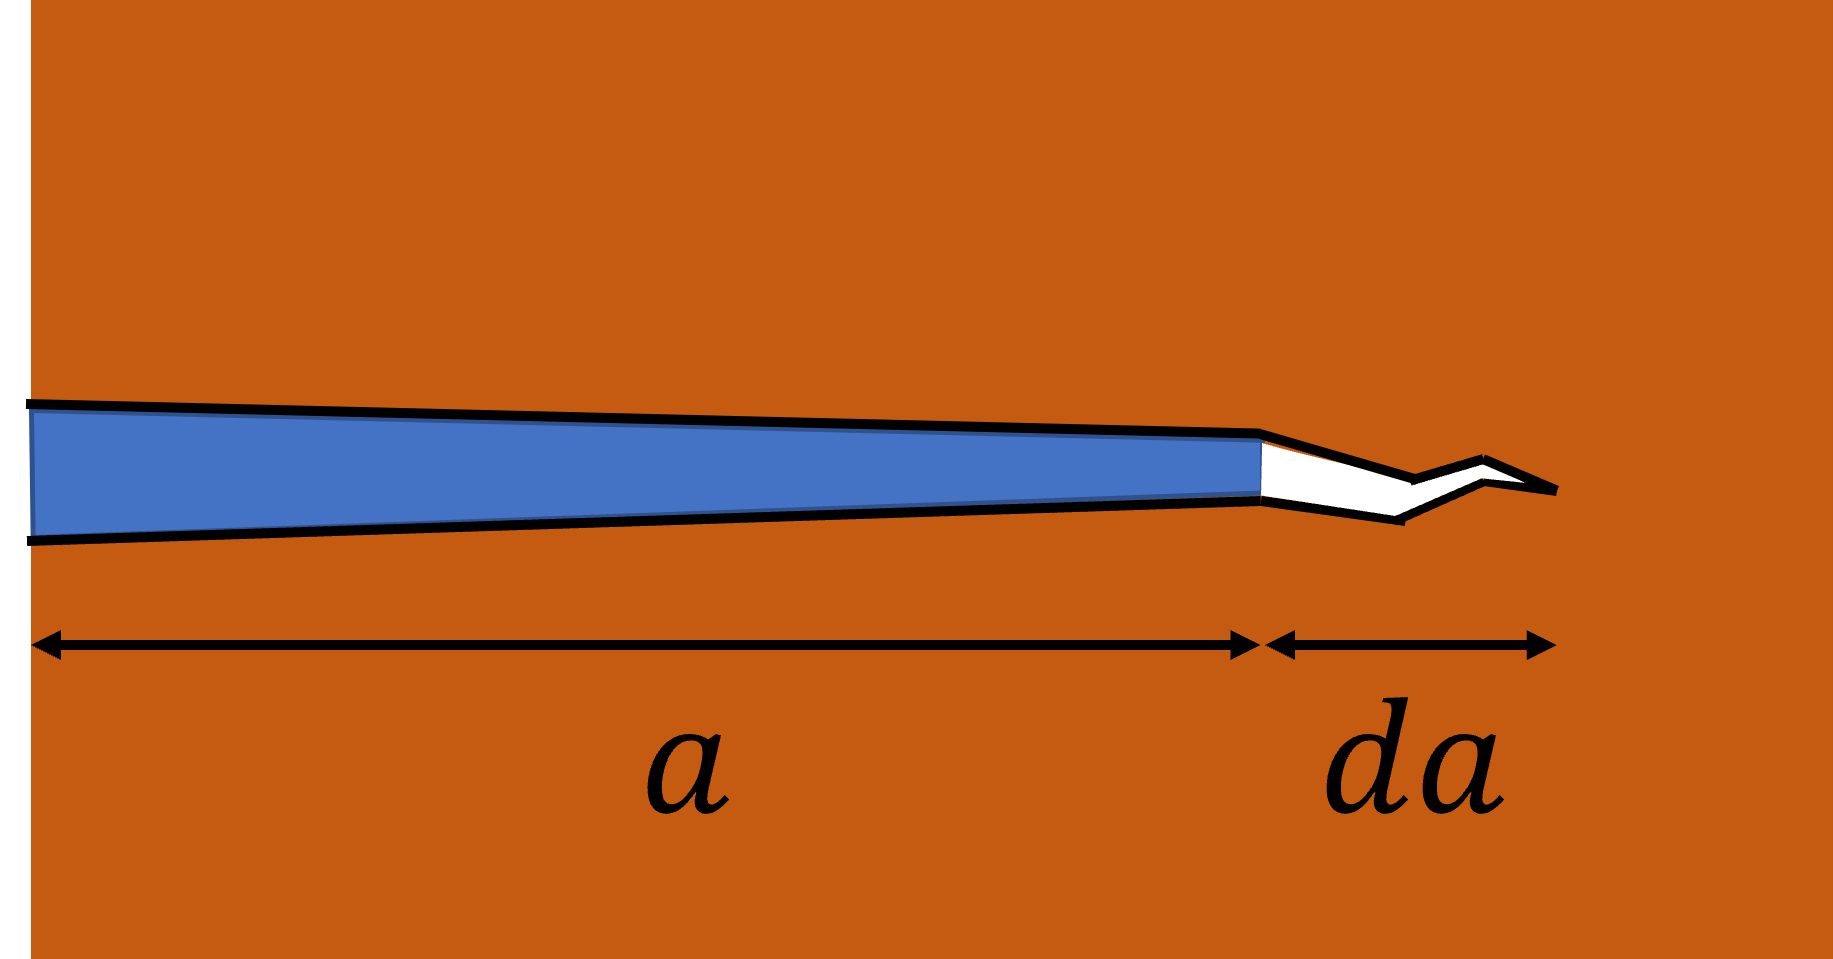
\includegraphics[width=0.9\linewidth]{images/theory_part/dry_crack.png}
  \caption{}
  \label{fig:dry_crack}
\end{subfigure}%
\begin{subfigure}{.49\textwidth}
  \centering
  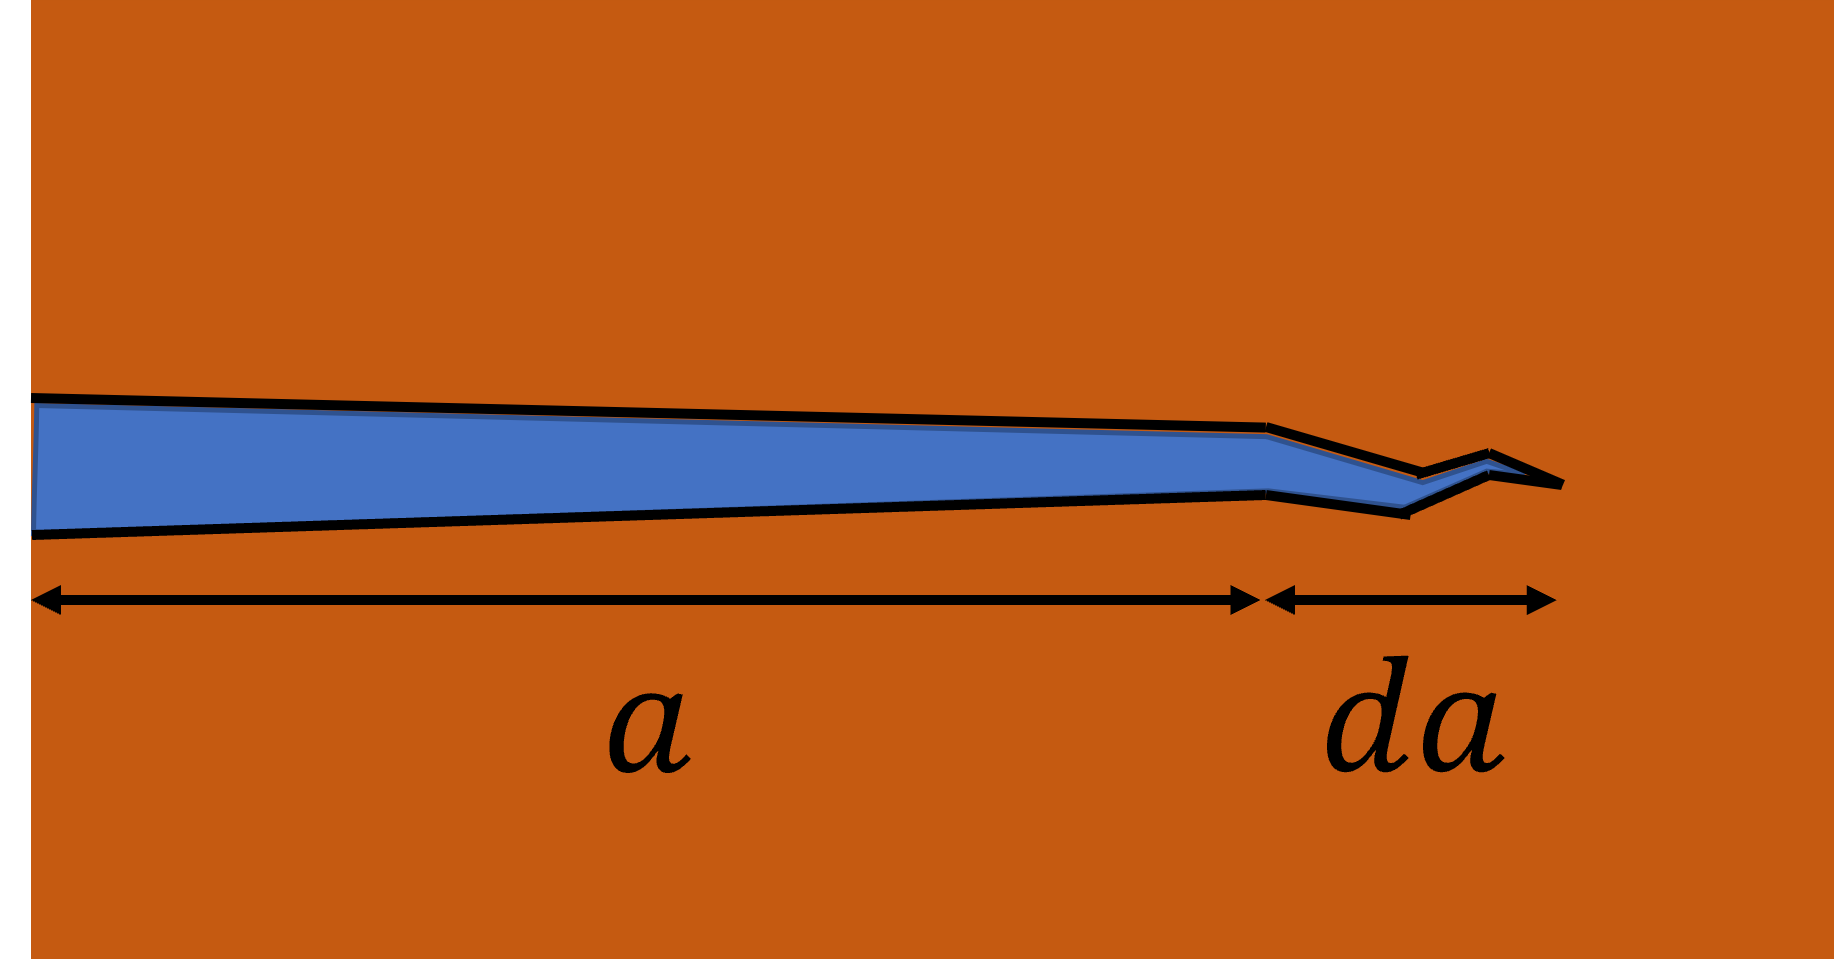
\includegraphics[width=0.9\linewidth]{images/theory_part/wet_crack.png}
  \caption{}
  \label{fig:wet_crack}
\end{subfigure}%
  \caption{(a) Unloaded virtual crack. (b) Pressure loaded virtual crack;} 
  \label{fig:wet_vs_dry_crack}
\end{figure}

In what follows, the formulation associated with Figure \ref{fig:dry_crack} will be referred to as the Unloaded Virtual Crack formulation, or UVC for short. In the UVC, the variation of the pressure work is simply\footnote{\noindent On the other hand, if the assumption of Figure \ref{fig:wet_crack} is chosen, as in \cite{bourdin2012variational}, two additional terms have to be accounted for, \begin{equation*}\label{wet variation}
    \delta \left( \int\limits_{\Omega} p \nabla d\cdot\textbf{u}\ I'(d)\text{dV} \right) = \int\limits_{\Omega} p \nabla d\cdot\delta\textbf{u}\ I'(d)\text{dV} \underbrace{+ \int\limits_{\Omega} p \nabla \delta d\cdot\textbf{u}\ I'(d)\text{dV} + \int\limits_{\Omega} p \nabla d\cdot\textbf{u}\ \delta d\ I''(d)\text{dV}}_{\text{additional terms}}.
\end{equation*}},

\begin{equation}\label{dry variation}
    \delta \left( \int\limits_{\Omega} p \nabla d\cdot\textbf{u}\ I'(d)\text{dV} \right) = \int\limits_{\Omega} p \nabla d\cdot\delta\textbf{u}\ I'(d)\text{dV}.
\end{equation}

\noindent The variation of the potential energy $\delta U$ can then be written as,

\begin{multline}
    \delta U(\bs{\epsilon},d) = \int\limits_{\Omega}\dfrac{\partial\psi_e}{\partial \bs \epsilon}:\delta\bs\epsilon\ \text{dV} + \int\limits_{\Omega} p \nabla d\cdot\delta\textbf{u}I'(d)\ \text{dV} 
    - \int\limits_{\partial \Omega_N} \textbf{t}\cdot\delta\textbf{u} \ \text{dA} \\
    + \int\limits_{\Omega}g'(d) \psi_e^+(\bs\epsilon)\delta d\ \text{dV}
    + \int\limits_{\Omega}\dfrac{G_c}{c_0\ell}\bigg( \alpha'(d)\delta d + 2\ell^2\nabla d \cdot \nabla \delta d\bigg)\ \text{dV},
\end{multline}

\noindent and, with the help of the divergence theorem, 

\begin{multline}
    \delta U(\bs{\epsilon},d) = \int\limits_{\Omega}\biggl(-\nabla \cdot \dfrac{\partial\psi_e}{\partial \bs \epsilon} + pI'(d) \nabla d\biggr)\cdot\delta\textbf{u}\ \text{dV} \\
    + \int\limits_{\Omega}\left(g'(d) \psi_e^+(\bs\epsilon)
    + \dfrac{G_c}{c_0\ell}\alpha'(d) - \nabla \cdot\dfrac{2G_c\ell}{c_0}\nabla d \right)\delta d\ \text{dV} \\
    + \int\limits_{\partial \Omega_N}\biggl( \dfrac{\partial\psi_e}{\partial \bs \epsilon}\cdot\textbf{n}  -\textbf{t}\biggr)\cdot\delta\textbf{u} \ \text{dA}
    + \int\limits_{\partial\Omega} \dfrac{2G_c\ell}{c_0}(\textbf{n}\cdot\nabla d)  \delta d\ \text{dA}.
\end{multline}

The local minimization principle requires the variation of the potential energy $\delta U$ to be non-negative for any admissible state $\textbf{u},d$. In other words, $\delta U(\bs\epsilon, d) \ge 0$, giving rise to the following equation and boundary condition for $\textbf{u}$, since the variation of the displacement field $\delta \textbf{u}$ is arbitrary:

\begin{equation}\label{disp equation}
    -\nabla \cdot \bs \sigma  + pI'(d) \nabla d = \bs 0 \text{ in }\Omega,
\end{equation}

\begin{equation}\label{disp bcs}
    \bs\sigma \cdot \textbf{n} - \textbf{t} = \bs 0 \text{ in }\partial\Omega_N.
\end{equation}

\noindent In the above, $\bs\sigma$ denotes the Cauchy stress, defined as $\bs\sigma = \dfrac{\partial\psi_e}{\partial \bs \epsilon}$. 

For the damage variable, it is assumed that the process is irreversible, such that $\dot{d} \ge 0$.  As such, only positive variations in the damage are admissible, and $\delta U(\bs\epsilon, d) \ge 0$ implies

\begin{equation}\label{damage equation ch2}
    g'(d) \psi_e^+(\bs\epsilon)
    + \dfrac{G_c}{c_0\ell}\alpha'(d) - \nabla \cdot \dfrac{2G_c\ell}{c_0}\nabla d \ge 0 \text{ in }\Omega,
\end{equation}
\begin{equation}\label{damage bcs}
    \dfrac{2G_c\ell}{c_0}\textbf{n}\cdot \nabla d \ge 0 \text{ on }\partial\Omega.
\end{equation}

\noindent Equations \eqref{damage equation ch2} and \eqref{damage bcs} are identical to those in the standard phase-field model for traction-free cracks. This is the main difference between the new formulation and existing ones derived from deriving from \cite{bourdin2012variational} and \cite{wheeler2014augmented}, in which the governing equation for the damage field contains additional terms to account for the pressure loads on the virtual cracks. In what follows, we refer to that as the Loaded Virtual Crack formulation, or LVC.  In the boxes below, the governing equations for the UVC are compared to those of the LVC.  

\bigskip
\noindent
\begin{mdframed}[
    frametitle={\begin{equation}\label{uvc}\tag{UVC}\text{Unloaded Virtual Crack Formulation}\end{equation}},
    frametitlebackgroundcolor=gray!20,
    backgroundcolor=gray!5,
    linewidth=0pt,
    nobreak=true
  ]
  
\begin{equation}\label{disp equation box}
    -\nabla \cdot \bs\sigma  + pI'(d) \nabla d = \bs 0 \text{ in }\Omega,
\end{equation}

\begin{equation}\label{disp bcs box}
    \bs\sigma\cdot \textbf{n} -\textbf{t} = \bs 0 \text{ in }\partial\Omega_N.
\end{equation}

\begin{equation}\label{damage equation box}
    g'(d) \psi_e^+(\bs\epsilon)
    + \dfrac{G_c}{c_0\ell}\alpha'(d) - \nabla \cdot \dfrac{2G_c\ell}{c_0}\nabla d \ge 0 \text{ in }\Omega,
\end{equation}

\begin{equation}\label{damage bcs box}
    \dfrac{2G_c\ell}{c_0}\textbf{n}\cdot \nabla d \ge 0 \text{ on }\partial\Omega.
\end{equation}
  
\end{mdframed}
%\end{minipage}
\hspace{.03\linewidth}
%\begin{minipage}{.48\linewidth}
\begin{mdframed}[
    frametitle={\begin{equation}\label{lvc}\tag{LVC}\text{Loaded Virtual Crack Formulation}\end{equation}},
    frametitlebackgroundcolor=gray!20,
    backgroundcolor=gray!5,
    linewidth=0pt,
    nobreak=true
  ]
  
\begin{equation}\label{disp equation box2}
    -\nabla \cdot \bs\sigma  + pI'(d) \nabla d = \bs 0 \text{ in }\Omega,
\end{equation}

\begin{equation}\label{disp bcs box2}
    \bs\sigma\cdot \textbf{n} - \textbf{t} = \bs 0 \text{ in }\partial\Omega_N.
\end{equation}

\begin{multline}\label{wet damage equation box2}
    g'(d) \psi_e^+(\bs\epsilon)
    + \dfrac{G_c}{c_0\ell}\alpha'(d) - \nabla \cdot \dfrac{2G_c\ell}{c_0}\nabla d \\ - \nabla \cdot [p\textbf{u}\ I'(d)] + p\nabla d\cdot \textbf{u}I''(d) \ge 0 \text{ in }\Omega,
\end{multline}
    
\begin{equation}\label{wet damage bcs box2}
    \textbf{n}\cdot \left(\dfrac{2G_c\ell}{c_0}\nabla d+   pI'(d)\textbf{u}\right) \ge 0 \text{ on }\partial\Omega.
\end{equation}
  
\end{mdframed}

\noindent It is readily apparent that the governing equations for the displacements are identical in the UVC and the LVC. The main difference is in the absence of the additional pressure-dependent terms in the evolution for the damage field and the accompanying boundary condition.  

In Appendix \ref{SIF_equivalence}, an analytical study of the energy release rate of a crack propagating under an arbitrary pressure load $p(x)$ is provided, under the assumptions of the UVC formulation and linear elastic fracture mechanics. The results of the study show that it is possible to recover the classic relationship between the energy release rate and the stress intensity factor with the UVC formulation. This ensures the consistency of the proposed formulation \eqref{uvc} with many theoretical works \cite{detournay2016mechanics, garagash2000tip, detournay2004propagation, garagash2005plane, bunger2005toughness} in the field of hydraulic fracture, where the stress intensity factor is used as the propagation criterion.

\subsection{Derivation using the maximum dissipation principle}\label{dyn_derivation}

In this subsection, an alternative approach to derive the \eqref{uvc} formulation  is presented. It is based on the construction of a total potential functional which depends on the rates of the internal variables $\dot{\bs\epsilon},\dot{d}$ and accounts for  the work of the pressure load as an external dissipation mechanism. This approach is described in more detail in \cite{hu2021variationalpaper} and \cite{hu2021variationalthesis}, where it is used to derive a variationally consistent phase-field model for ductile fracture. 

The total potential is postulated as,

\begin{equation}\label{total potential}
    L(\dot{\bs\epsilon},\dot{d}) = \int\limits_{\Omega} \dot{u}(\dot{\bs\epsilon},\dot{d}) \text{dV} - \mathcal{P}^{ext}, 
\end{equation}
where $u$ is the material internal energy, which relates to the Helmholtz free-energy $\psi$ through $\dot{u} = \dot{\psi} + \dot{T}s$, where $T$ is the temperature and $s$ the entropy. 
In this work, only isothermal processes are considered, therefore, $\dot{u} = \dot{\psi}$. The term $\mathcal{P}^{ext}$ denotes the external power expenditure. If cracks were represented by internal boundaries $\Gamma$ instead of a damage field, one could write,

\begin{equation}\label{power expenditure}
    \mathcal{P}^{ext} = \int\limits_{\partial \Omega \cup \Gamma} \textbf{t}\cdot\dot{\textbf{u}} \text{dA} = \int\limits_{\partial \Omega} \textbf{t}\cdot\dot{\textbf{u}}\text{dA} + \int\limits_{\Gamma} p\textbf{n}\cdot\dot{\textbf{u}} \text{dA}.
\end{equation}

\noindent However, in a regularized setting this integral over $\Gamma$ is once again transformed into a volume integral over $\Omega$, as in \eqref{reg pressure term}, 

\begin{equation}\label{reg power expenditure}
    \int\limits_{\Gamma} p\textbf{n}\cdot\dot{\textbf{u}} \text{dA} \approx \int\limits_{\Omega} p \left( -\frac{\nabla d}{\Vert\nabla d\Vert} \right)\cdot\dot{\textbf{u}} \Vert\nabla I(d)\Vert\text{dV} = 
    -\int\limits_{\Omega}p\nabla d \cdot\dot{\textbf{u}} I'(d) \text{dV}.
\end{equation}

Recalling the equivalence between the internal energy and the Helmholtz free-energy, the Coleman-Noll procedure can be applied and, in combination with \eqref{power expenditure} and \eqref{reg power expenditure}, leads to the following expression for $L$ as a function of $\psi$: 

\begin{equation}
    L(\dot{\bs\epsilon},\dot{d}) = \int\limits_{\Omega} \left( \dfrac{\partial\psi}{\partial\bs\epsilon}:\dot{\bs\epsilon} + \dfrac{\partial\psi}{\partial d}\dot{d}+\dfrac{\partial\psi}{\partial \nabla d}\cdot {\nabla \dot d} + p\nabla d \cdot\dot{\textbf{u}} I'(d) \right) \text{dV} - \int\limits_{\partial \Omega} \textbf{t}\cdot\dot{\textbf{u}} \text{dA}. 
\end{equation}

The evolution process is postulated to follow the minimizers of this total potential, with the supplemental conditions that damage is an irreversible process and that the displacements $\textbf{u}$ are prescribed over a subset $\partial \Omega_D$ of the boundary. In other words, 

\begin{equation}\label{minimization principle}
    \dot{\bs\epsilon}, \dot{d} = \underset{\dot{\bs\epsilon},\dot{d}}{{\operatorname{argmin}}} \ L(\dot{\bs\epsilon}, \dot{d}) \text{,\ \   subject to } \dot{d} \ge 0 \text{ and } \textbf{u}=\textbf{g} \text{ on }\partial \Omega_D. 
\end{equation}

\noindent Using the Euler-Lagrange equations, the following general evolution equations can then be obtained in terms of the free-energy function $\psi$:
\begin{equation}\label{u_equation}
    \nabla \cdot \dfrac{\partial\psi}{\partial \bs\epsilon} - pI'(d) \nabla d = \bs 0 \text{ in }\Omega,
\end{equation}
\begin{equation}\label{d_equation}
    \nabla \cdot \dfrac{\partial\psi}{\partial \nabla d} - \dfrac{\partial\psi}{\partial d} \ge \bs 0 \text{ in }\Omega,
\end{equation}
with the boundary conditions
\begin{equation}\label{u_bc_helmholtz}
    \dfrac{\partial\psi}{\partial \bs\epsilon}\cdot\textbf{n} - \textbf{t} = \bs 0 \text{ on }\partial\Omega\setminus\partial\Omega_D
\end{equation}
\begin{equation}\label{d_bc_helmholtz}
    \textbf{n} \cdot \dfrac{\partial\psi}{\partial \nabla d} \ge 0 \text{ on }\partial\Omega.
\end{equation}

\noindent To be consistent with the derivation in subsection \ref{qs_derivation}, the Helmholtz free-energy is postulated as,

\begin{equation}\label{helmholtz free-energy postulate}
    \psi(\bs{\epsilon},d) = \psi_e(\bs{\epsilon},d) + \dfrac{G_c}{c_0\ell}\bigg( \alpha(d) + \ell^2\nabla d \cdot \nabla d\bigg),
\end{equation}

\noindent following the regularization based on the Ambrosio-Tortorelli functional. In this case, the general equations \eqref{u_equation}-\eqref{d_bc_helmholtz} take the form
\begin{equation}
\label{eq:UVC-eq2}
    -\nabla \cdot \bs\sigma  + pI'(d) \nabla d = \bs 0 \text{ in }\Omega,
\end{equation}
\begin{equation}
    g'(d) \psi_e^+(\bs\epsilon)
    + \dfrac{G_c}{c_0\ell}\alpha'(d) - \nabla \cdot \dfrac{2G_c\ell}{c_0}\nabla d \ge 0 \text{ in }\Omega,
\end{equation}
 with the boundary conditions
\begin{equation}
    \bs\sigma\cdot \textbf{n}-\textbf{t} = \bs 0 \text{ on }\partial\Omega_N,
\end{equation}
\begin{equation}
\label{eq:UVC-bc2}
    \textbf{n}\cdot \nabla d \ge 0 \text{ on }\partial\Omega.
\end{equation}
By inspection, \eqref{eq:UVC-eq2}-\eqref{eq:UVC-bc2} are identical to \eqref{disp equation}-\eqref{damage bcs}.

\subsection{Constitutive choices of the phase-field formulation}

In the previous subsection, the proposed model for pressurized cracks was developed for a general phase-field regularization of the variational approach to fracture \cite{francfort1998revisiting}, with a free-energy of the form

\begin{equation}\label{PF general form}
    \psi(\bs{\epsilon},d) = \underbrace{g(d)\psi_e^+(\bs{\epsilon}) + \psi_e^-(\bs{\epsilon})}_{\psi_e} + \underbrace{\frac{G_c}{c_0\ell}\bigg( \alpha(d) + \ell^2\nabla d \cdot \nabla d\bigg)}_{\psi_f}.
\end{equation}

\noindent where $\psi_f$ is used to indicate the part of the free-energy associated with fracture. In what follows, the constitutive choices used in the example problems provided in Section \ref{sec:results} are described. 

\subsubsection{Elastic energy and decomposition}

First, in terms of the solid bulk response, an elastic energy of the type \eqref{energy split} is assumed. When the material is undamaged, it reduces to a purely linear elastic energy, that is,

\begin{equation}
    \psi_e(\bs\epsilon(\textbf{u}),0) = \psi_e^+(\bs\epsilon(\textbf{u}),0)+\psi_e^-(\bs\epsilon(\textbf{u}),0) = \dfrac{1}{2}\bs\epsilon(\textbf{u}) : \mathbb{C} : \bs\epsilon(\textbf{u}),
\end{equation}

\noindent where $\mathbb{C}$ is the elasticity tensor.

When damage is present, a decomposition of the energy is often assumed. In many cases, when the applied load to a fracturing body is predominately tensile, the ``no-split" case given by,

\begin{equation}
    \psi_e^-(\bs\epsilon(\textbf{u}),d)=0 \rightarrow \psi_e(\bs\epsilon(\textbf{u}),d) = \dfrac{1}{2}g(d)\bs\epsilon(\textbf{u}) : \mathbb{C} : \bs\epsilon(\textbf{u}),
\end{equation}

\noindent is capable of correctly predicting the material response, while leading to a simpler set of governing equations. However, in a wide range of scenarios, compressive forces are present, and an energy split is needed to prevent crack formation in zones of high compression, as well as to allow for transmission of compressive forces across fractured faces. 

In Section \ref{sec:results}, one of the example problems will employ the spectral split of Miehe et al. \cite{miehe2010phase},  given by,

\begin{equation}
    \psi_e^+(\bs\epsilon(\textbf{u}),d) = \dfrac{1}{2}\lambda\left<\text{Tr }\bs\epsilon\right>_+^2+\mu\bs\epsilon^+:\bs\epsilon^+ \text{ and }  \psi_e^-(\bs\epsilon(\textbf{u}),d) = \dfrac{1}{2}\lambda\left<\text{Tr }\bs\epsilon\right>_-^2+\mu\bs\epsilon^-:\bs\epsilon^-.
\end{equation}

Here, $\left< \cdot \right>_+$ and $\left< \cdot \right>_-$ denote the positive and negative parts of a number respectively, while $\bs\epsilon^+$ and $\bs\epsilon^-$ are the positive and negative parts of an additive decomposition of the strain tensor based on the signs of its eigenvalues. A more detailed description, including the derivation of the stiffness matrix in this case, is provided by Jiang et al.\ \cite{jiang2020three}.

\subsubsection{Brittle fracture}

The first and more traditional phase-field model with an energy of the type \eqref{PF general form} was proposed in \cite{bourdin2000numerical}. It was developed to approximate the brittle fracture process of linear elastic materials in the limit of vanishing $\ell$. In its original form, the degradation function 

\begin{equation}\label{quadratic_degradation}
    g(d) = \xi + (1-\xi)(1-d)^2,
\end{equation}

\noindent is used in combination with a quadratic local dissipation $\alpha(d) = d^2$, in what is now called the AT-2 formulation. However, the use of, $\alpha(d) = d$, (widely referred as the AT-1) comes with the advantage of a purely elastic response before the onset of damage and a compactly supported damage field. Therefore, it will be employed in the example in Section \ref{sec:results} where brittle fracture is investigated. The parameter $\xi$ in \eqref{quadratic_degradation} is the residual stiffness, a very small numerical parameter that avoids the loss of ellipticity in fully damaged material.

\subsubsection{Cohesive fracture}\label{cohesive_frac}

The phase-field model for cohesive fracture was first proposed by Lorentz et al. \cite{lorentz2011convergence, lorentz2011gradient}. In this model, the use of a quasi-quadratic degradation function, given by
\begin{equation}\label{cohesive_degradation}
    g(d) = \xi + (1-\xi)\dfrac{(1-d)^2}{(1-d)^2+md(1+pd)},
\end{equation}
is combined with a linear local dissipation function $\alpha(d) = d$.  The parameter $m$ is defined as $m = \dfrac{G_c}{c_0\ell\psi_c}$, where $\psi_c$ is the nucleation energy, below which no damage is expected to form.  The parameter $p$ is a shape parameter that can be used to adjust the traction-separation response.  In this work, $p=1$ is used.  

\section{A J-Integral for pressurized cracks in a phase-field setting}\label{sec:j_integral}

%In the field of Fracture Mechanics, a very important tool for assessing the phenomena of propagation is the so-called J-Integral \cite{rice1968mathematical, rice1968path, rice1973some}. {\color{purple}This contour integral, in its basic form, is path independent and provides a simple way to retrieve the energy release rate of a given mechanical configuration.} When a phase-field description of fracture is used, in most of the time, an explicit computation of the energy release rate is not necessary, as the balance between elastic and fracture energy is enforced by the variational principle. {\color{purple}Nevertheless, with certain modifications, the J-Integral can also be applied in the regularized setting as a verification tool, as in \cite{hossain2014effective, kumar2020revisiting}.}

%With respect to the novel model described in Section \ref{sec:model}, it is important to assess how well it satisfies Griffith's law for finite values of $\ell$ and whether it converges as $\ell \rightarrow 0$. For this purpose, it is necessary to extract the instantaneous energy release rate (here denoted as $G$) of pressurized cracks in a phase-field context. 

This Section presents a modified J-Integral, capable of retrieving the energy release rate, denoted here by $G$ in the case of pressurized cracks in a phase-field for fracture setting. The resulting integral is then re-cast into a domain-independent form that is more amenable to finite-element calculations.  
 

%{\color{purple}This J-Integral is re-cast in the domain form, which has a few advantages compared to the contour form. First, the implementation is simpler when used in the finite element context, as it only needs integration over elements, allowing standard quadrature rules to be used. Second, it also retains improved accuracy, since it does not require interpolation of quantities outside of quadrature points.} 

%The first use of the J-Integral in the context of phase-field fracture dates back to the work of Hakim and Karma \cite{hakim2009laws}, who used it to study the fracture model proposed in \cite{karma2001phase}. Later, in \cite{sicsic2013gradient} and \cite{ballarini2016closed} the concept was applied to the phase-field model based on the regularization of the variational approach to fracture of Francfort and Marigo \cite{francfort1998revisiting}. In these works, the expression of the J-Integral, which works in general, for traction-free cracks is,

A common form of the J-Integral, derived for phase-field fracture and applicable to traction-free cracks is given by \cite{sicsic2013gradient,ballarini2016closed} 
\begin{equation}
    J = \textbf{r} \cdot \int\limits_{\zeta} \biggl( \psi(\bs\epsilon, d)\mathbb{I} - \nabla \textbf{u}^T\bs \sigma-\nabla d \otimes \bs\omega \biggr) \textbf{n}\text{ds}, 
\end{equation}
where $\psi(\bs\epsilon, d)$ is given by equation \eqref{PF general form}. In the above, the vector $\textbf{r}$ denotes the crack propagation direction, $\zeta$ is a closed path around the crack tip, $\mathbb{I}$ is the second-order identity tensor, $\textbf{n}$ is the normal to the closed path $\zeta$ and $\bs\omega = \partial \psi/\partial \nabla d = (G_c\ell/c_0)\nabla d$. Compared to the original form of the J-Integral proposed by Rice~\cite{rice1968mathematical,rice1968path}, this expression contains additional terms to account for the phase-field parameter $d$. 

Importantly,  Sicsic and Marigo \cite{sicsic2013gradient} show that, under certain conditions, the standard form of the J-Integral widely employed for sharp cracks, viz.
\begin{equation}
    J = \textbf{r} \cdot \int\limits_{\zeta} \biggl( \psi_e(\bs\epsilon, d)\mathbb{I} - \nabla \textbf{u}^T\bs \sigma\biggr) \textbf{n}\text{ds},
\end{equation}
 can be used in a regularized phase-field setting. These conditions are:

\begin{enumerate}[start=1,label={\bfseries H\arabic*}]
    \item \label{itm:hyp1}: The regularization length is sufficiently small, so that a separation of scales between the solution in the damage band and the outer solution can be achieved;

    \item \label{itm:hyp2}: The path $\zeta$ intersects the crack plane at a ninety-degree angle;

    \item \label{itm:hyp3}: The path $\zeta$ intersects the crack plane sufficiently far from the crack tip, so that the damage field only varies in a direction perpendicular to the crack plane.   
\end{enumerate}

\noindent In what follows, these same conditions are assumed, as they facilitate a simpler derivation of a modified J-Integral capable of retrieving the energy release rate even in the presence of pressure loads on the crack faces. The main result of this section can then be stated in the following way.

% \begin{figure}[h]
%     \centering
%     \begin{tikzpicture}
%         \node {\pgfimage[interpolate=false,width=.4\textwidth]{images/theory_part/potato_crack.png}};
%         \draw (-0.1\textwidth,-0.1\textwidth) node {\LARGE$\Omega$};
%         \draw (0.03\textwidth,0.03\textwidth) node {\LARGE\color{blue}$p$};
%         \draw (0.075\textwidth,-0.05\textwidth) node {\LARGE$\Gamma$};
%         \draw (0.16\textwidth,0.16\textwidth) node {\LARGE$\textbf{t}$};
%     \end{tikzpicture}
%     \caption{Generic body containing cracks loaded in pressure.}
%     \label{fig:potato}
% \end{figure}

\begin{figure}[ht]
% \centering
\begin{subfigure}{.49\textwidth}
  \centering
  % \begin{tikzpicture}
  %       \node {\pgfimage[interpolate=false,width=.8\textwidth]{images/theory_part/j_integral.png}};
  %       \draw (-0.18\textwidth,-0.1\textwidth) node {\LARGE$\Lambda$};
  % \end{tikzpicture}
  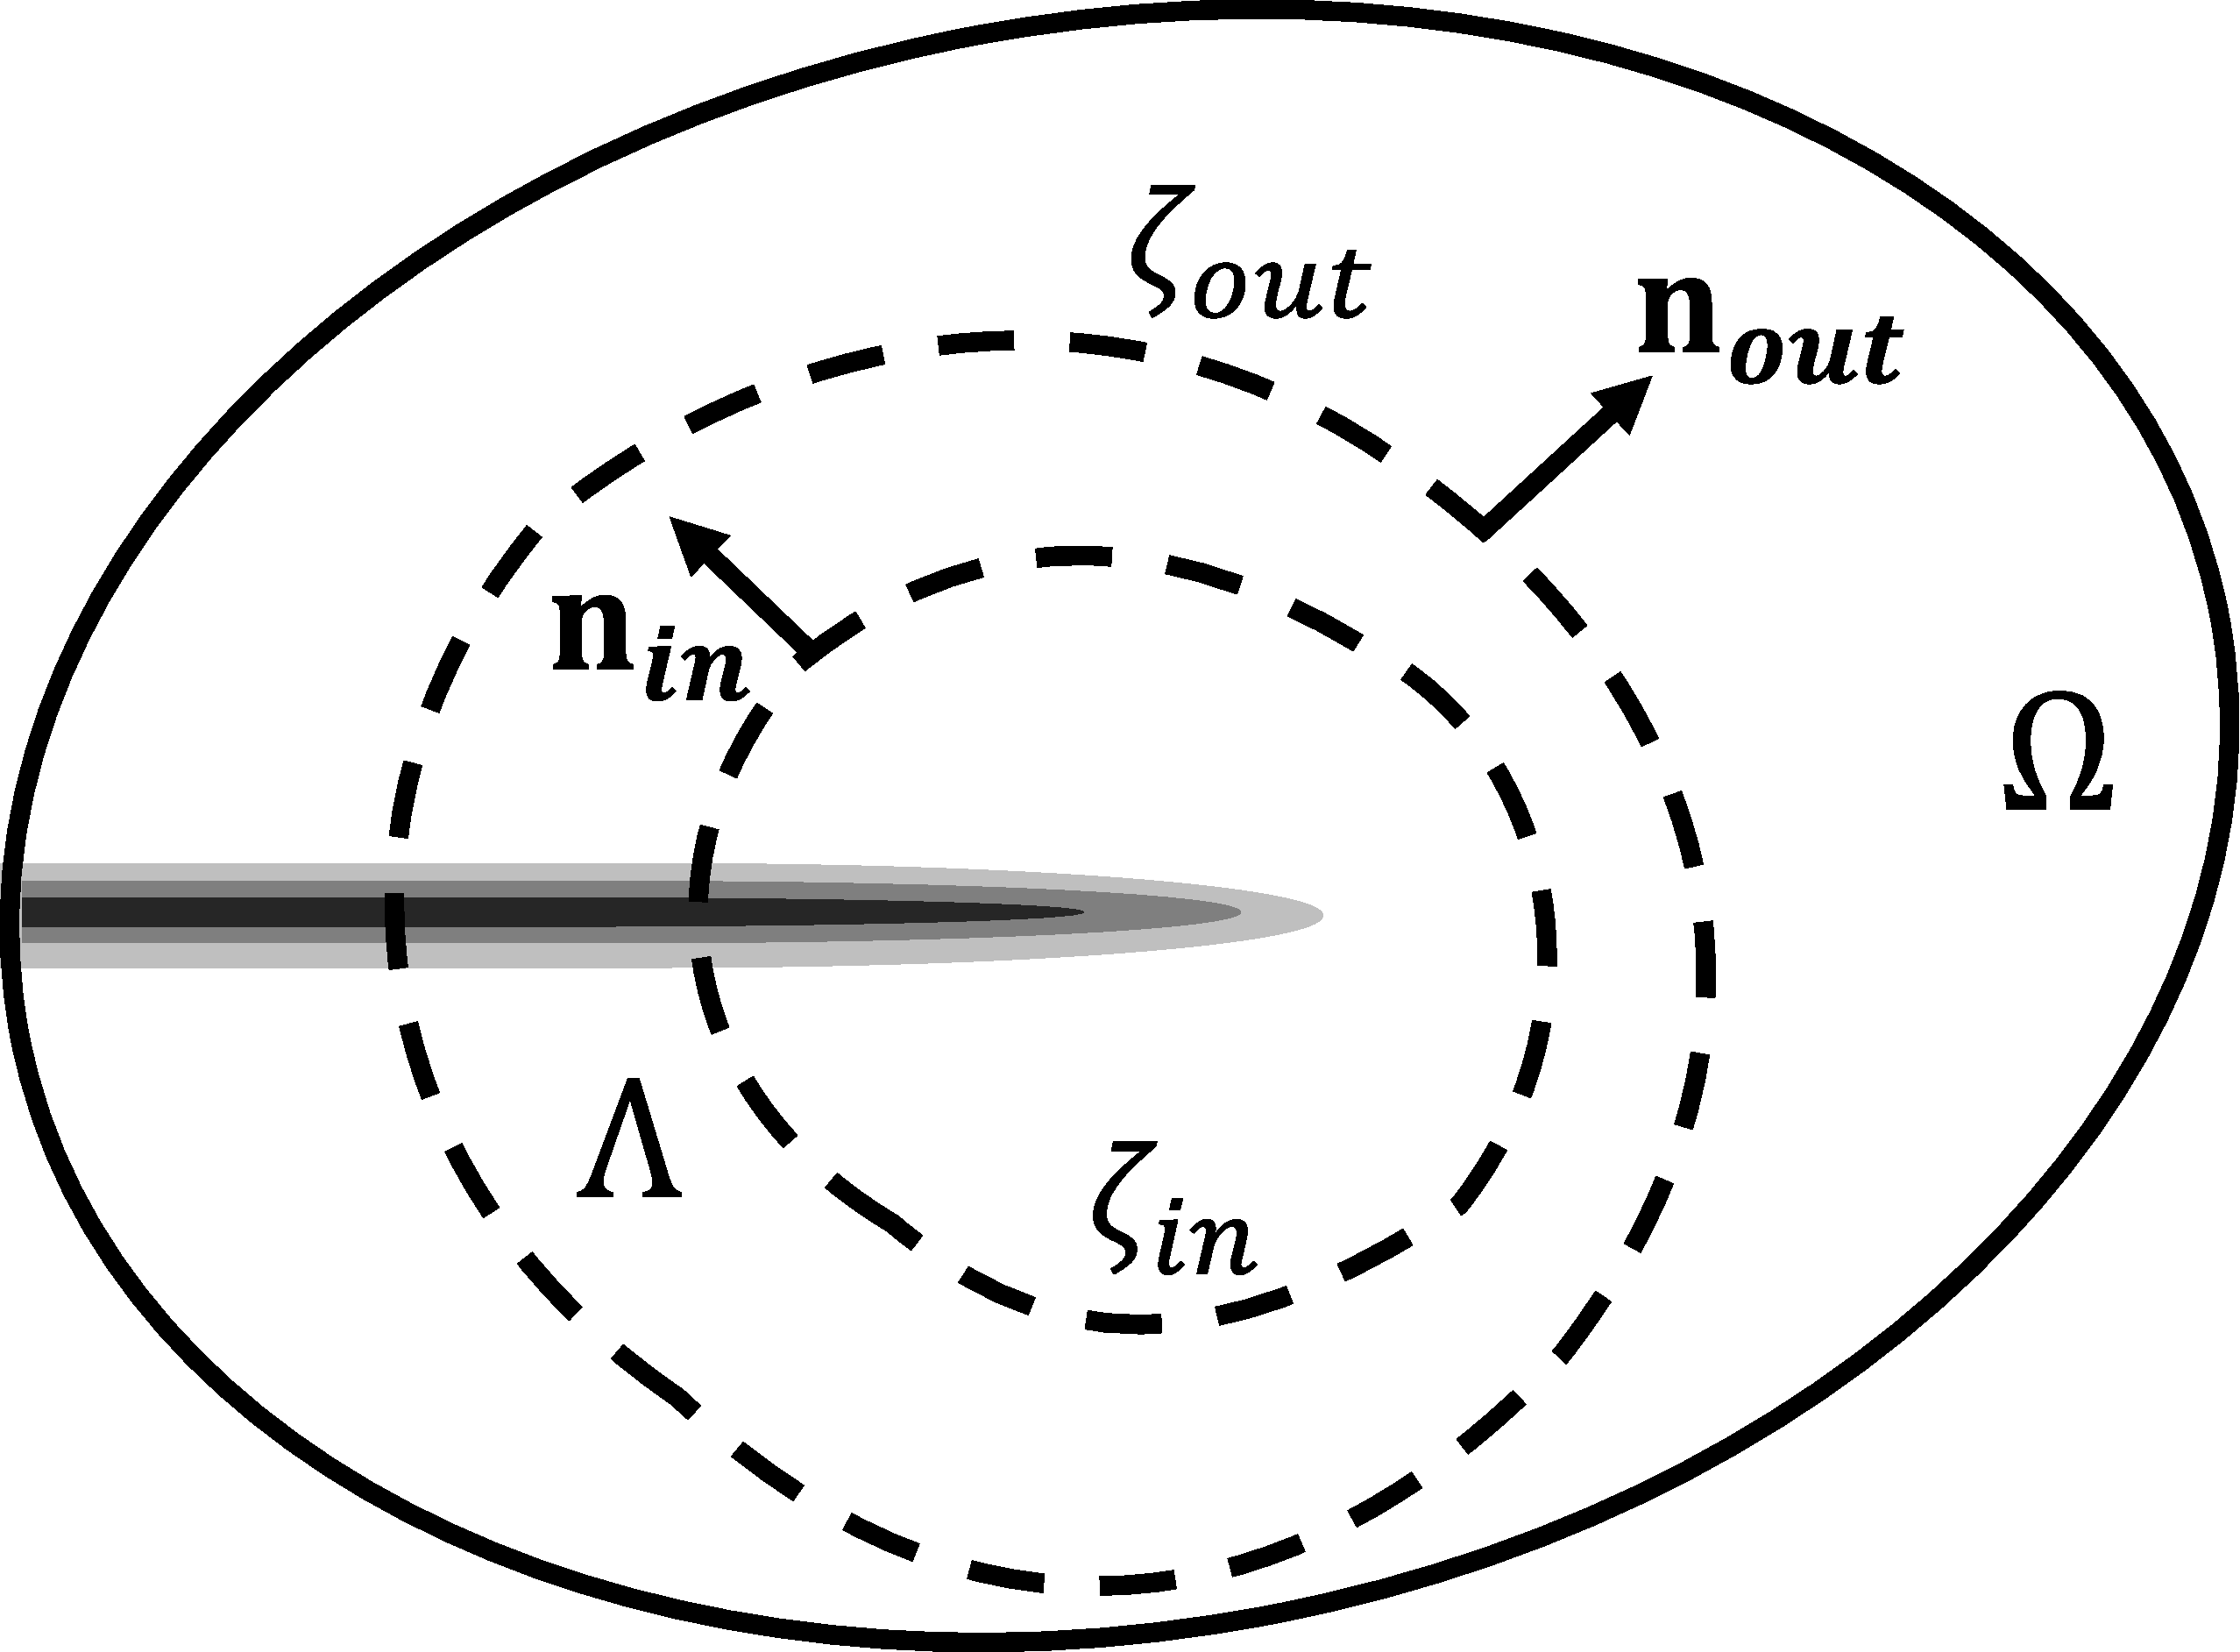
\includegraphics[width=0.8\linewidth]{images/theory_part/j_integral_bw.pdf}
  \bigskip
  \bigskip
  \caption{}
  \label{fig:j_integral}
\end{subfigure}%
\begin{subfigure}{.49\textwidth}
  \centering
  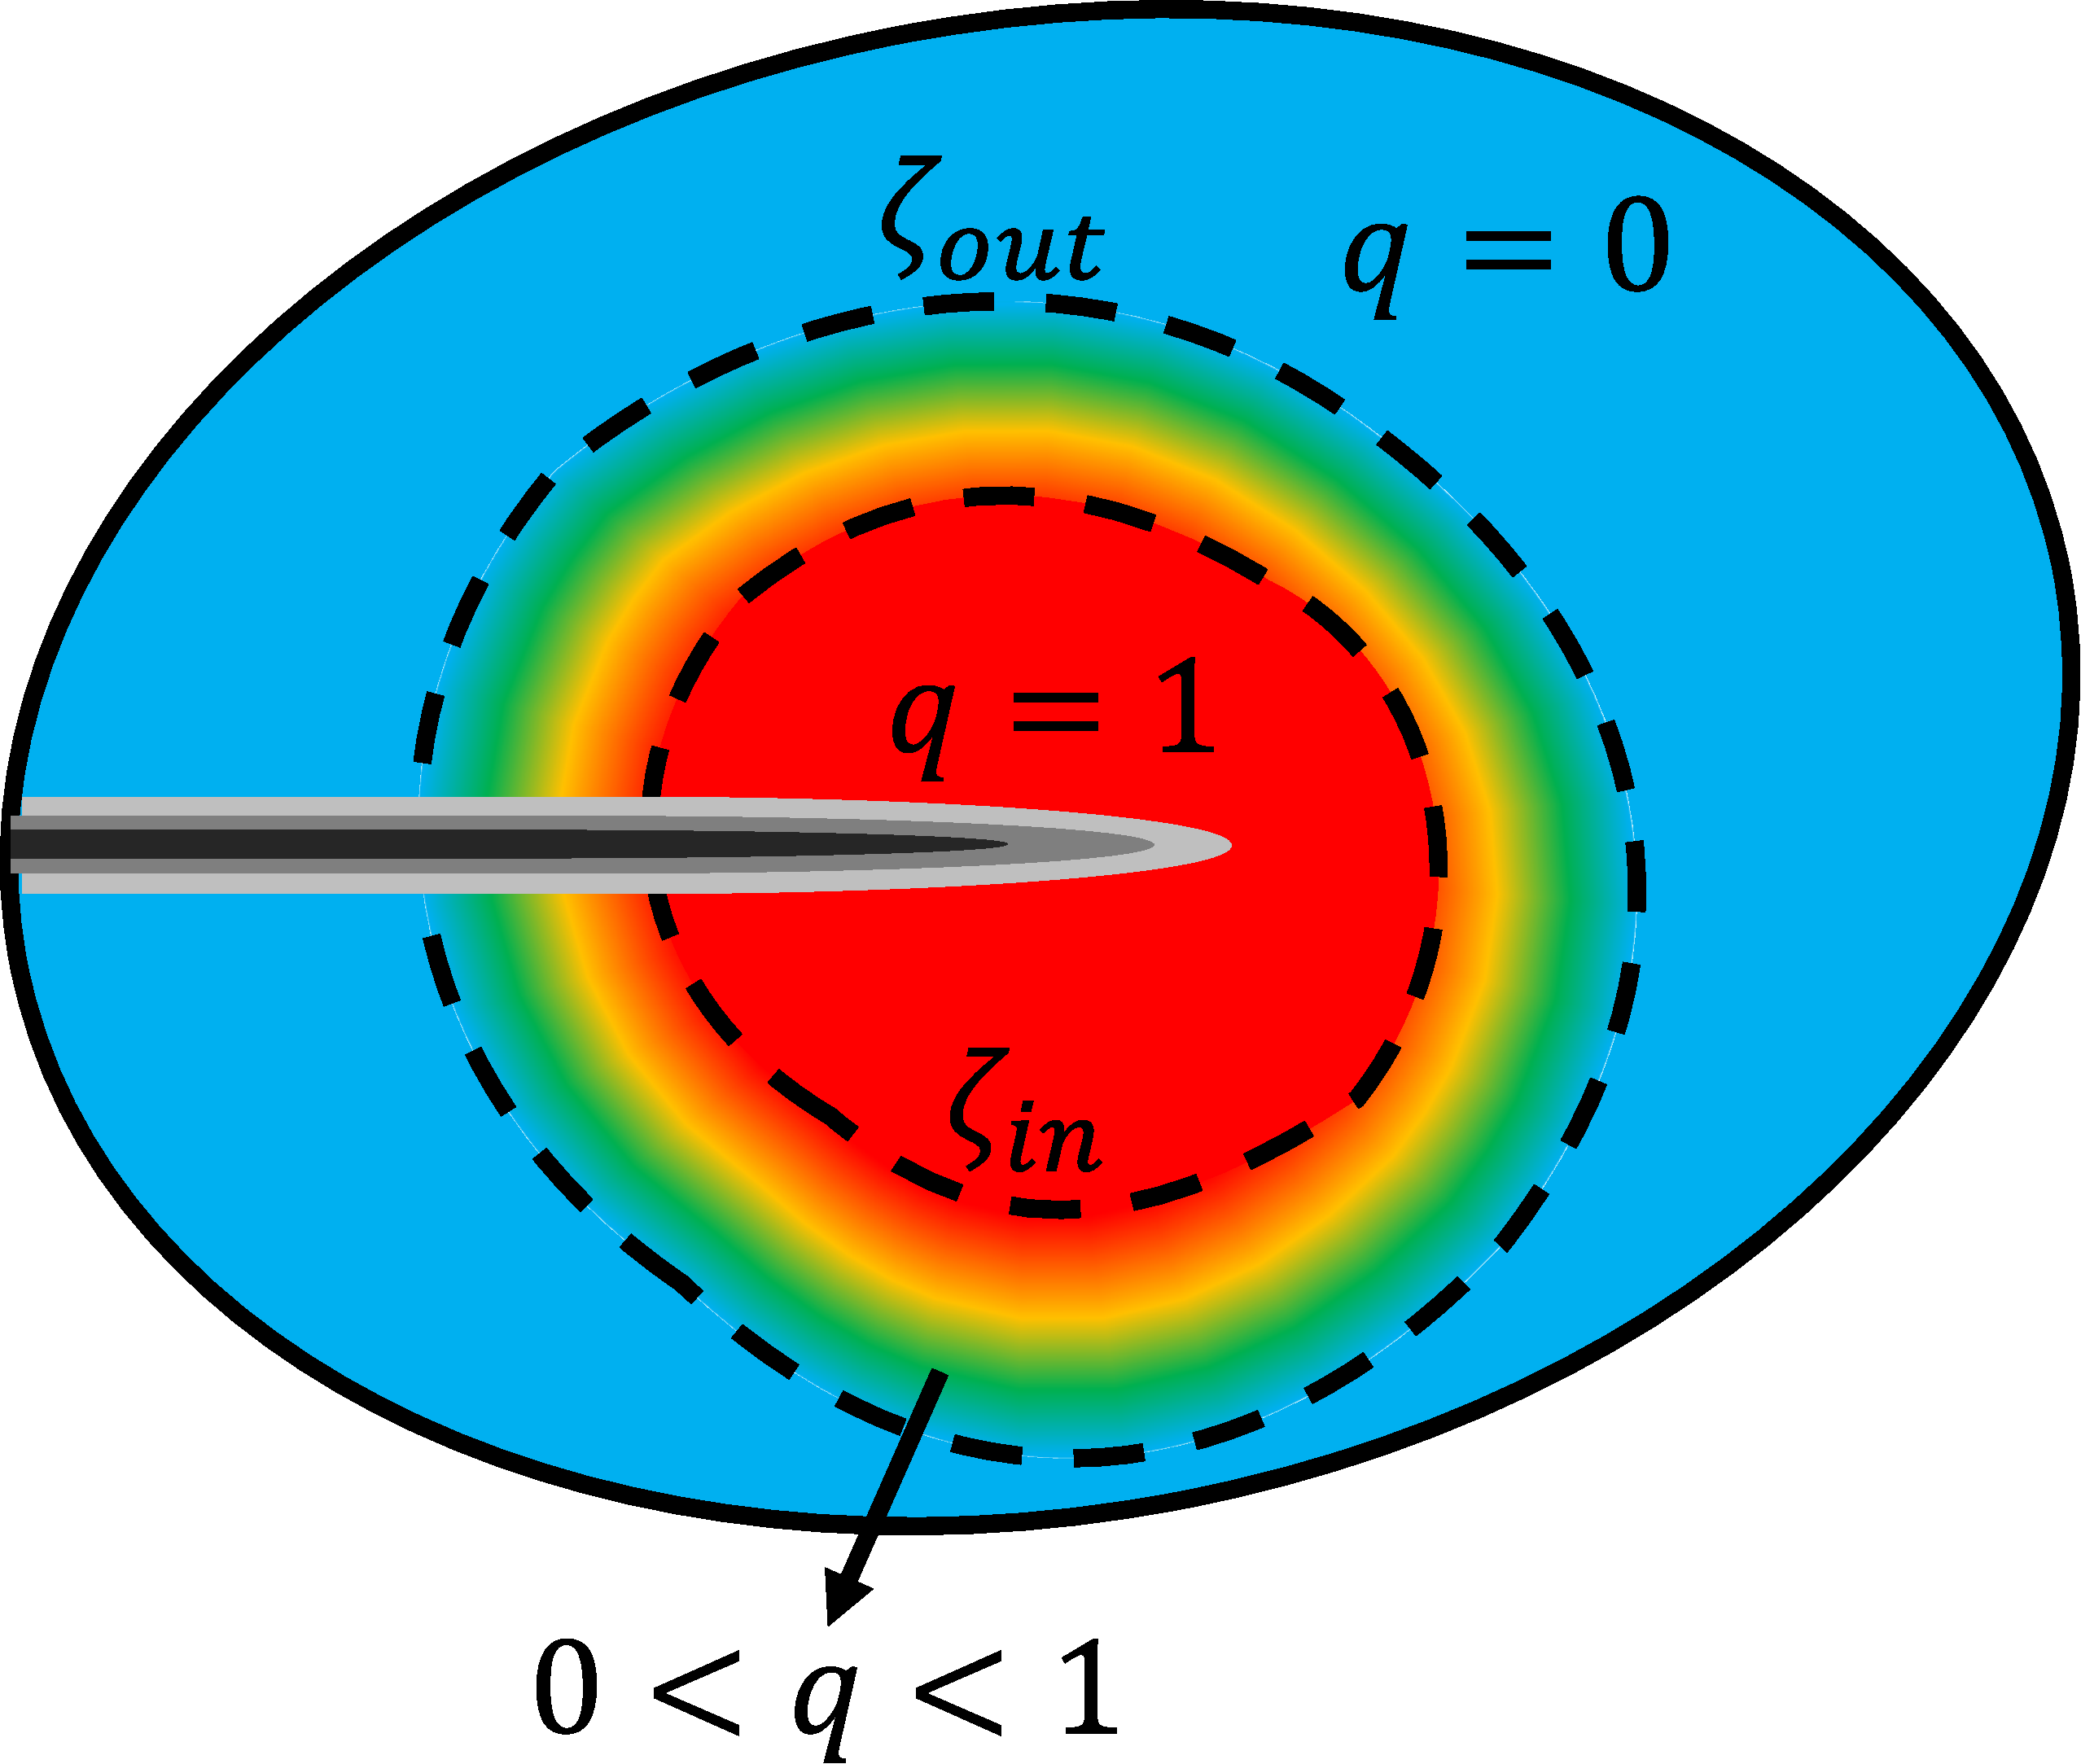
\includegraphics[width=0.8\linewidth]{images/theory_part/j_integral_bw_q.pdf}
  \caption{}
  \label{fig:j_integral_q}
\end{subfigure}%
  \caption{(a) The contour paths $\zeta_{in}$ and $\zeta_{out}$ and subdomain $\Lambda$, in the vicinity of a regularized crack.; (b) Color contour plot indicating the assumed variation in the function $q$.  } 
  \label{fig:j_integral_pics}
\end{figure}

% \begin{figure}[ht]
% % \centering
% \begin{subfigure}{.49\textwidth}
%   \centering
%   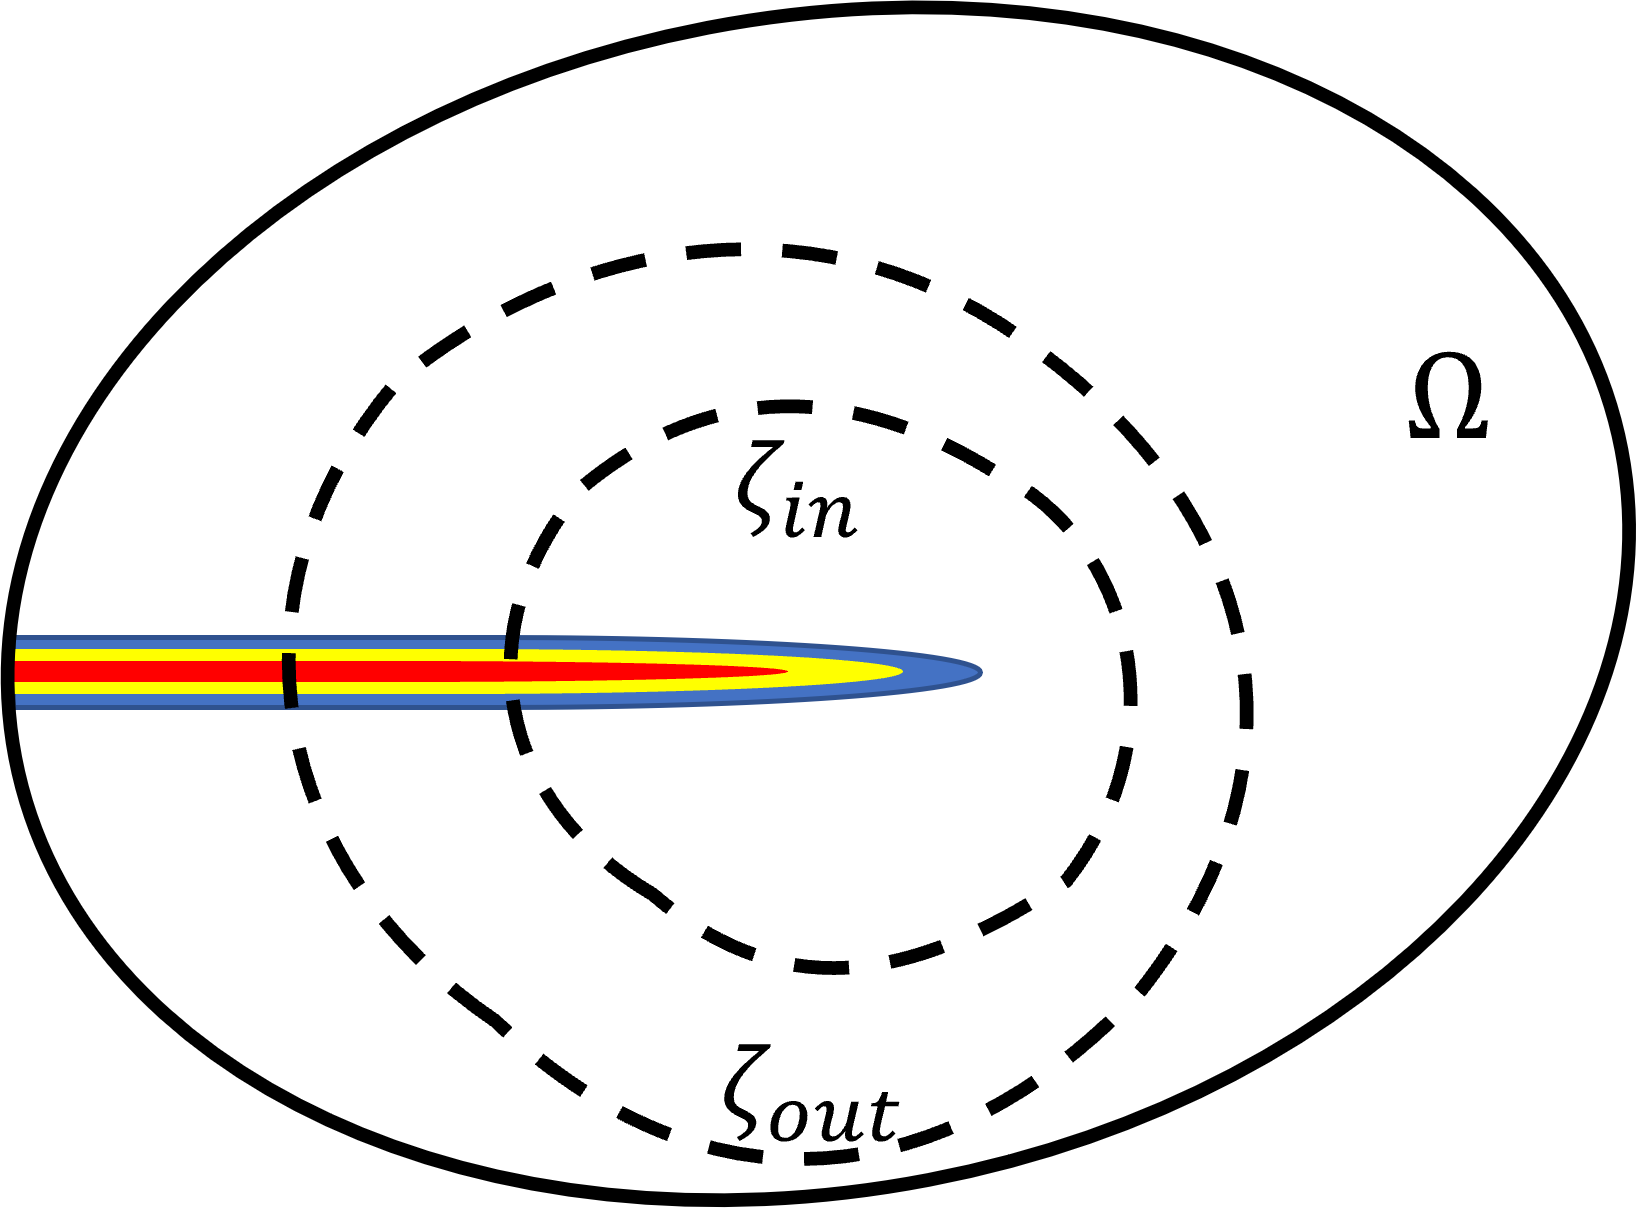
\includegraphics[width=0.8\linewidth]{images/theory_part/j_integral.pdf}
%   \bigskip
%   \bigskip
%   \caption{}
%   \label{fig:j_integral}
% \end{subfigure}%
% \begin{subfigure}{.49\textwidth}
%   \centering
%   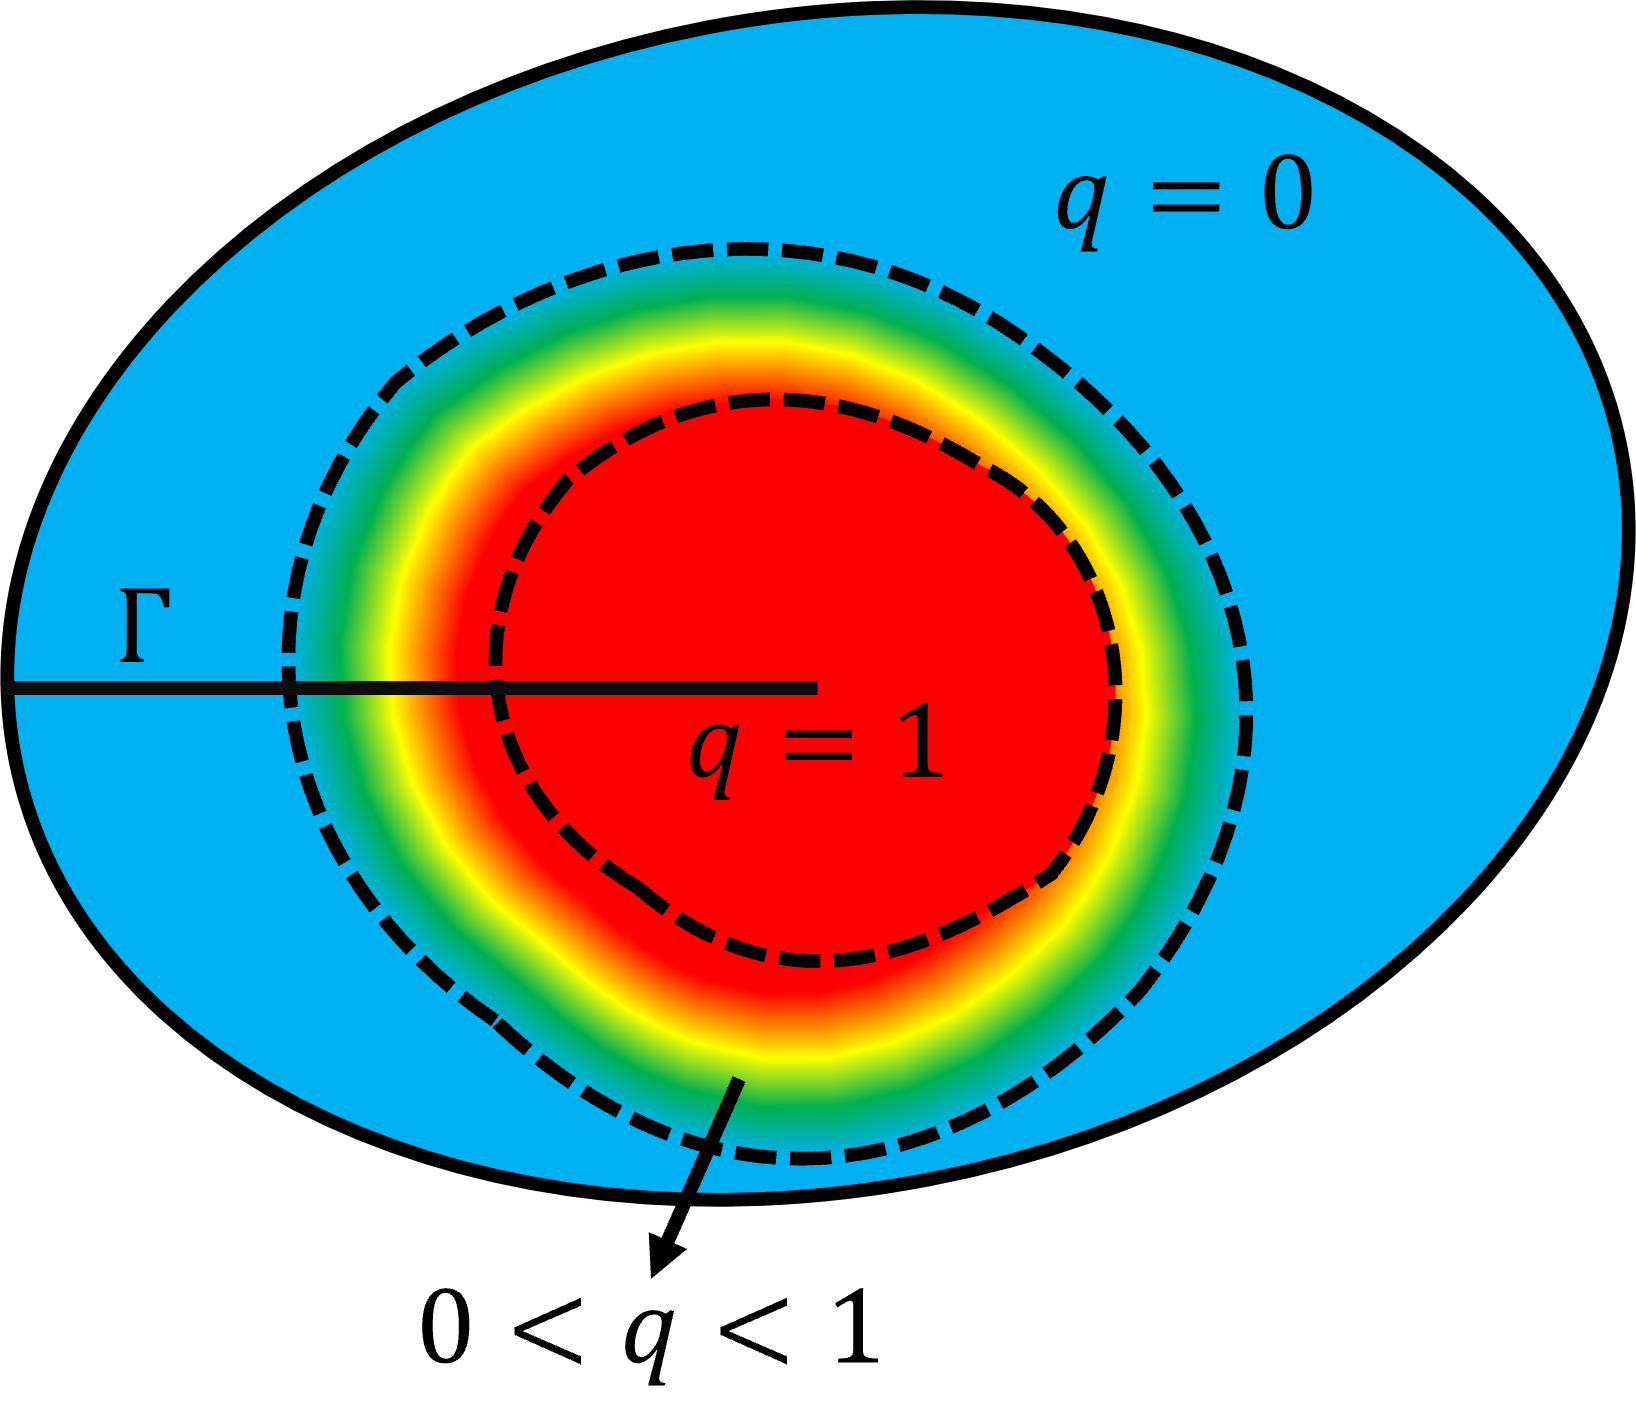
\includegraphics[width=0.8\linewidth]{images/theory_part/j_integral_q.pdf}
%   \caption{}
%   \label{fig:j_integral_q}
% \end{subfigure}%
%   \caption{(a) Description of paths $\zeta_{in}$ and $\zeta_{out}$.; (b) Description of the function $q$. ADD $\Lambda$ TO FIRST FIGURE.} 
%   \label{fig:j_integral_pics}
% \end{figure}

\medskip

\noindent\textbf{Claim}: Consider a domain $\Omega \in \mathbb{R}^2$ with a straight phase-field crack and two closed, non-intersecting paths $\zeta_{in}$ and $\zeta_{out}$ around the crack tip, enclosing an area $\Lambda$ as shown in Figure~\ref{fig:j_integral}. Let $q(x)$ be a sufficiently smooth function satisfying $q = 1$ on $\zeta_{in}$ and $q = 0$ on $\zeta_{out}$. Further, assume that $q = 1$ for all points inside $\zeta_{in}$ and $q = 0$ for all points outside $\zeta_{out}$, as shown in Figure \ref{fig:j_integral_q}. Finally, assume that the fracture is loaded by a constant pressure $p$, and that one of the formulations described in Section \ref{sec:model} holds. Then, if conditions \ref{itm:hyp1}, \ref{itm:hyp2} and \ref{itm:hyp3} hold for $\zeta_{in}$ and $\zeta_{out}$, the energy release rate can be approximated by the  integral
\begin{equation}\label{j_integral_theorem}
    J = \textbf{r} \cdot \int\limits_{\Lambda} \biggl( \psi_e(\bs\epsilon, d)\mathbb{I} -p\nabla d\cdot\textbf{u}I'(d)\mathbb{I}  - \nabla \textbf{u}^T\bs \sigma \biggr) \cdot \nabla q\ \text{dA},
\end{equation}

\noindent with an error that vanishes as $\ell \rightarrow 0$. The proof can be established in three steps, as detailed below.

\medskip

\noindent \textbf{Proof:} Define $\textbf{T}_p = \psi_e(\bs\epsilon, d)\mathbb{I} -p\nabla d\cdot\textbf{u}I'(d)\mathbb{I}  - \nabla \textbf{u}^T\bs \sigma$. Using the divergence theorem, one can show that
\begin{equation}
    \int\limits_{\Lambda} \nabla\cdot(q\textbf{T}_p)\text{dA} = \int\limits_{\zeta_{in}\cup\zeta_{out}}q\textbf{T}_p\cdot\textbf{n}\ \text{ds} = 0 - \int\limits_{\zeta_{in}}\textbf{T}_p\cdot\textbf{n}\ \text{ds}, 
\end{equation}
because $q$ vanishes on $\zeta_{out}$ and the normal $\textbf{n}$ to $\zeta_{in}$ points inward to $\Lambda$, as shown in Figure~\ref{fig:j_integral}.  
%sign change in the last term is due to the orientation of the normal $\textbf{n}$. 
Multiplying both sides by the crack direction $\textbf{r}$ and applying the chain rule yields
\begin{equation}\label{first_step}
    -\textbf{r}\cdot\int\limits_{\Lambda} \biggl( \textbf{T}_p\cdot \nabla q + q\nabla \cdot \textbf{T}_p\biggr)\text{dA} =  \textbf{r}\cdot\int\limits_{\zeta_{in}}\textbf{T}_p\cdot\textbf{n}\ \text{ds}, 
\end{equation}
 which completes the first step of the proof. 
 
 The second step consists of showing that the term $R = \textbf{r}\cdot\int\limits_{\Lambda} q\nabla \cdot \textbf{T}_p\ \text{dA}$ is zero. Expanding the expression for $\textbf{T}_p$ and using the chain rule yields
\begin{multline}
    R = \textbf{r}\cdot\int\limits_{\Lambda} q\nabla \cdot \biggl( \psi_e(\bs\epsilon, d)\mathbb{I} -p\nabla d\cdot\textbf{u}I'(d)\mathbb{I}  - \nabla \textbf{u}^T\bs\sigma \biggr)\ \text{dA} \\ = \int\limits_{\Lambda} q\biggl( \dfrac{\partial \psi_e(\bs\epsilon, d)}{\partial\nabla^s\textbf{u}}\cdot(\nabla(\nabla^s\textbf{u})\textbf{r}) + \dfrac{\partial \psi_e(\bs\epsilon, d)}{\partial d}\nabla d\cdot \textbf{r}
    - (\nabla \cdot \bs\sigma)\cdot(\nabla\textbf{u}\textbf{r}) \\ - \bs\sigma(\nabla (\nabla\textbf{u})\textbf{r})-p\nabla d\cdot(\nabla \textbf{u}\textbf{r})I'(d) - p\textbf{u}\nabla(I'(d)\nabla d)\textbf{r} \biggr)\ \text{dA}.
\end{multline}
 Re-arranging some terms, one can write,
\begin{multline}
    R = \int\limits_{\Lambda} q\biggl[\biggl( \dfrac{\partial \psi_e(\bs\epsilon, d)}{\partial\nabla^s\textbf{u}}-\bs\sigma\biggr) \cdot(\nabla(\nabla^s\textbf{u})\textbf{r}) 
    -\biggl( \nabla \cdot \bs\sigma - pI'(d) \nabla d \biggr)\cdot (\nabla\textbf{u}\textbf{r})
    \\ + \dfrac{\partial \psi_e(\bs\epsilon, d)}{\partial d}\nabla d\cdot \textbf{r}
    - p\textbf{u}\nabla(I'(d)\nabla d)\textbf{r} \biggr]\ \text{dA}.
\end{multline}

\noindent For any elastic material, the definition of stress implies $\dfrac{\partial \psi_e(\bs\epsilon, d)}{\partial\nabla^s\textbf{u}} = \bs\sigma$, and due to equation \eqref{u_equation}, $\nabla \cdot \bs\sigma - p \nabla d = \bs 0$, so, the expression above reduces to
\begin{equation}
    R = \int\limits_{\Lambda} q\biggl(\dfrac{\partial \psi_e(\bs\epsilon, d)}{\partial d}\nabla d\cdot \textbf{r} 
    - p\textbf{u}\nabla(I'(d)\nabla d)\textbf{r} \biggr)\ \text{dA}.
\end{equation}
Assuming a separation of scales, the domain $\Lambda$ can be separated into two regions: (i) $\Lambda_{band}$, which consists of the intersection between $\Lambda$ and the support of the damage field representing the crack and (ii) $\Lambda_{outer}$, which denotes the remainder of $\Lambda$, outside of the damage band.  In the asymptotic limit as $\ell\rightarrow 0$, the material in $\Lambda_{outer}$ behaves as purely elastic. Within $\Lambda_{outer}$, one has $d \approx \nabla d \approx 0$, and therefore,  
\begin{equation}
    R_{outer}  = \int\limits_{\Lambda_{outer}} q\biggl(\dfrac{\partial \psi_e(\bs\epsilon, d)}{\partial d}\nabla d\cdot \textbf{r} - p\textbf{u}\nabla(I'(d)\nabla d)\textbf{r} \biggr)\ \text{dA} \approx 0.
\end{equation}
 For the $\Lambda_{band}$ region, by condition \ref{itm:hyp3}, $\nabla d$ is purely perpendicular to the crack direction, so, $\nabla d \cdot \textbf{r} \approx 0$. Therefore,
\begin{equation}
    R_{band} = \int\limits_{\Lambda_{band}} q\biggl(\dfrac{\partial \psi_e(\bs\epsilon, d)}{\partial d}\nabla d\cdot \textbf{r} 
    - p\textbf{u}\nabla(I'(d)\nabla d)\textbf{r} \biggr)\ \text{dA} \approx 0.
\end{equation}


\noindent Since $\Lambda = \Lambda_{band} \cup \Lambda_{outer}$, we must have 

\begin{equation}\label{step2}
    R = R_{outer}+R_{band} \approx 0.
\end{equation}

\noindent This completes the second step. 


The final step of the proof begins by invoking the separation of scales to decompose the contour integral in \eqref{first_step} via
\begin{equation}\label{step3}
    \textbf{r}\cdot\int\limits_{\zeta_{in}}\textbf{T}_p\cdot\textbf{n}\ \text{ds} = \textbf{r}\cdot\biggl(\int\limits_{\zeta^{band}_{in}}\textbf{T}_p\cdot\textbf{n}\ \text{ds} + \int\limits_{\zeta^{outer}_{in}}\textbf{T}_p\cdot\textbf{n}\ \text{ds} \biggr).
\end{equation}
On the $\zeta^{outer}_{in}$ portion of the path, damage effects can be neglected and the integral simplifies to the standard (sharp) J-Integral.  In the case of a uniformly pressurized crack \cite{karlsson1978jintegral}, this gives
% \noindent On the $\zeta^{outer}_{in}$ portion of the path, the second term in the right side of \eqref{step3} reduces to the expression of Rice's J-Integral, which, in the case of a uniformly pressurized crack \cite{karlsson1978jintegral}, evaluates to,
\begin{equation}\label{path_outer}
    \int\limits_{\zeta^{outer}_{in}}\textbf{T}_p\cdot\textbf{n}\ \text{ds} = G - pw,
\end{equation}
where $w$ denotes the crack aperture at the intersection of the crack and the contour $\zeta_{in}$. 

The other portion of the integral can be re-written as
\begin{equation}
    \textbf{r}\cdot \int\limits_{\zeta^{band}_{in}}\textbf{T}_p\cdot\textbf{n}\ \text{ds} = \textbf{r}\cdot\int\limits_{-B}^{B}(\psi_e\mathbb{I}-\nabla \textbf{u}^T\bs\sigma)\cdot\textbf{n}dx - \textbf{r}\cdot\int\limits_{-B}^{B}p(\nabla d\cdot \textbf{u}I'(d))\cdot\textbf{n}dx,
\end{equation}

\noindent where $B$ is the half-length of the damage band and condition \ref{itm:hyp2} is used to transform the integral over $\zeta^{band}_{in}$ to a simple real integral from $-B$ to $B$. Here, both $\textbf{r}$ and $\textbf{n}$ are unit vectors that point in opposite directions, and therefore, $\textbf{r}\cdot\textbf{n}=-1$, so,

\begin{equation}
    \textbf{r}\cdot \int\limits_{\zeta^{band}_{in}}\textbf{T}_p\cdot\textbf{n}\ \text{ds} = \int\limits_{-B}^{B}(\psi_e\mathbb{I}-\nabla \textbf{u}^T\bs\sigma)dx + p\int\limits_{-B}^{B}(\nabla d\cdot \textbf{u}I'(d))dx.
\end{equation}
Following \cite{bourdin2012variational}, the second integral on the right approaches the crack aperture $w$ as the regularization length decreases, while the first integrand on the right is bounded \cite{sicsic2013gradient}, and therefore this term is $O(B)$, so,

\begin{equation}\label{path_band}
    \textbf{r}\cdot \int\limits_{\zeta^{band}_{in}}\textbf{T}_p\cdot\textbf{n}\ \text{ds} = O(B) + pw = O(\ell) + pw,
\end{equation}

\noindent since the damage band half-length $B$ scales with the regularization length $\ell$. One can now go back to \eqref{step3}, and substitute \eqref{path_outer} and \eqref{path_band} to obtain,

\begin{equation}\label{third_step}
    \textbf{r}\cdot\int\limits_{\zeta_{in}}\textbf{T}_p\cdot\textbf{n}\ \text{ds} = G + pw - pw + O(\ell).    
\end{equation}

\noindent Finally, combining \eqref{first_step}, \eqref{step2} and \eqref{third_step}, one obtains

\begin{equation}\label{end_step}
    -\textbf{r}\cdot\int\limits_{\Lambda}  \textbf{T}_p\cdot \nabla q\ \text{dA} =  G + O(\ell), 
\end{equation}

\noindent which concludes the proof.





\section{Finite Element Implementation}
\label{sec:fem_implementation}

In this Section, the details of the finite element discretization used to obtain approximations to the solution of the proposed model \eqref{uvc} are described. For analogous equations for the model \eqref{lvc}, the reader is referred to \cite{jiang2022phase}.
%The method of choice is the finite element method, as in most of the works regarding the phase-field approach for fracture. 
First, the strong form of the governing equations, derived from the general free-energy \eqref{PF general form} using the KKT\cite{karush1939minima, kuhn1951nonlinear} conditions is presented.

% To obtain approximate solutions to the proposed model, we will use the finite element method. In order to lay out the equations for the approximate solution, let's first start by re-writing the strong form of the problem with our choice of free-energy (\ref{PF general form}). 

\begin{mdframed}[
  frametitle={Strong form},
  frametitlebackgroundcolor=gray!20,
  backgroundcolor=gray!5,
  linewidth=0pt,
  nobreak=true
  ]
  \vspace{-1em}
  \begin{align}
    \text{Linear momentum balance: } & \nabla \cdot \bs\sigma -p\nabla d + \textbf{b} = 0,                       &  & \forall x \in \Omega,                          \\
                                     & \bs\sigma = \frac{\partial\psi_e}{\partial \bs\epsilon},                   &  & \forall x \in \Omega, \\
                                     & \bs\sigma\cdot \textbf{n} = \textbf{t},                                          &  & \partial_t\Omega,  
                                     \\
                                     & \textbf{u} = \textbf{u}_g,                                                      &  & \partial_u\Omega ,                \\
    \text{Fracture evolution: }      & \dot d\left(\nabla\cdot\frac{2G_c\ell}{c_0}\nabla d - \frac{G_c}{c_0\ell}\alpha'(d) - g'(d)\psi_e^+ (\bs\epsilon)\right) = 0,                                       &  & \forall x \in \Omega,           \\
    & \nabla \cdot \frac{2G_c\ell}{c_0}\nabla d - \frac{G_c}{c_0\ell}\alpha'(d) - g'(d)\psi_e^+ (\bs\epsilon) \le 0,                                       &  & \forall x \in \Omega,  \label{damage ineq}         \\
                                     & \dot d \ge  0,                                         &  & \forall x \in \Omega, \\
                                     & \nabla d\cdot\textbf{n}_0 = 0,                                         &  & \partial\Omega, \\
                                         & d(0,\textbf{x}) = d_0,                                         &  & \Omega.                                  
    \end{align}
\end{mdframed}

For the derivation of an equivalent weak form, trial spaces for $\textbf{u}$ and $d$ are first defined.  Although the derivation is confined to quasi-static loadings, the spaces are indexed by a discrete load step parameter $t$.   The trial spaces are given by

  \begin{align}
    \boldsymbol{\mathcal{U}}_t & = \{ \textbf{u} \in \mathcal{H}^1(\Omega)^d \mid \textbf{u} = \overline{\textbf{u}}_t \text{ on } \partial_u\Omega \}, \\
    \mathcal{D}_t      & = \{ d \in \mathcal{H}^1(\Omega) \mid d_{t-1}(x) \le d_t(x) \le 1,\ \forall x \in \Omega \}, 
  \end{align}

\noindent and the accompanying weighting spaces $\boldsymbol{\mathcal{V}}$ and $\mathcal{C}$ are

  \begin{align}
    \boldsymbol{\mathcal{V}} & = \{ \textbf{w} \in \mathcal{H}^1(\Omega)^d \mid \textbf{w} = \boldsymbol{0} \text{ on } \partial_u\Omega \}, \\
    \mathcal{C}      & = \{ c \in \mathcal{H}^1(\Omega) \mid c(x) \ge 0,\ \forall x \in \Omega \}.                                                     
  \end{align}

The condition of monotonicity in the space $\mathcal{D}_t$ is used to prevent damage healing and is the weak enforcement of the condition $\dot d \ge 0$, in a time discrete setting. Denoting the inner product in $\mathcal{H}^1(\Omega)$ and $\mathcal{H}^1(\Omega)^d$ by $\left( \cdot, \cdot \right)$ and it's restriction in the boundary by $\left<\cdot,\cdot\right>$, the weak form of the problem can be written as

% \footnote{ In this weak form, the inequality governing the damage evolution is written as an equality for simplicity. That is because in the solution strategy it is indeed treated as an equality but only over the active set, namely the set of points where $\dot d > 0$.}

\begin{mdframed}[
    frametitle={Weak form},
    frametitlebackgroundcolor=gray!20,
    backgroundcolor=gray!5,
    linewidth=0pt,
    nobreak=true
  ]
  Find $\textbf{u} \in \boldsymbol{\mathcal{U}}_t$ and $d \in \mathcal{D}_t$, such that $\forall \textbf{w} \in \boldsymbol{\mathcal{V}}$ and $\forall c \in \mathcal{C}$,
  
    \begin{align}
      \left( \nabla \textbf{w}, \bs\sigma \right) - \left( \textbf{w}, p\nabla d \right) - \left( \textbf{w}, \textbf{b} \right) - \left< \textbf{w}, \textbf{t} \right>_{\partial_t\Omega} & = 0, \\
      \frac{2\ell}{c_0}\left( \nabla c, G_c\nabla d \right) + \frac{1}{c_0\ell}\left( c, G_c\alpha'(d) \right) + \left( c, g'(d)\psi_e^+ (\bs\epsilon(\textbf{u})) \right) & = 0,\label{weak damage equation}
    \end{align}
 
\noindent with the initial damage condition,
 
    \begin{align}
      \left( c, d(0,\textbf{x}) - d_0 \right)                & = 0.
    \end{align}
 
\end{mdframed}

Observe that \eqref{weak damage equation} is an equality rather than an inequality, such as \eqref{damage ineq}.  This reflects a view ahead, toward discretization, where in the present work  the irreversibility constraint is enforced with an active-set strategy.  The active set strategy effectively partitions the domain into active (where $\dot{d}=0$) and inactive (where $\dot{d}>0$) parts. Only the inactive part requires a discretization of the damage condition \eqref{damage ineq}, where it is indeed treated as an equality. A detailed description of this constrained optimization algorithm is given by Heister et al. in \cite{heister2015primal}, and some additional details pertinent to phase-field for fracture discretizations can be found in Hu et al. \cite{hu2020phase}.

Finally, these function spaces can be discretized over a finite element mesh, that give rise to the discrete function spaces $\boldsymbol{\mathcal{U}}^h_t \subset \boldsymbol{\mathcal{U}}_t$, $\boldsymbol{\mathcal{V}}^h \subset \boldsymbol{\mathcal{V}}$, $\mathcal{D}^h_t \subset \mathcal{D}_t$, $\mathcal{C}^h \subset \mathcal{C}$. These are then used to construct the discrete form of the problem using the Galerkin method:

\begin{mdframed}[
    frametitle={Spatially discretized form},
    frametitlebackgroundcolor=gray!20,
    backgroundcolor=gray!5,
    linewidth=0pt,
    nobreak=true
  ]
  Find $\textbf{u}^h \in \boldsymbol{\mathcal{U}}^h_t$ and $d^h \in \mathcal{D}^h_t$, such that $\forall \textbf{w}^h \in \boldsymbol{\mathcal{V}}^h$ and $\forall q^h \in \mathcal{C}^h$,
  \begin{subequations}
    \begin{align}
      \left( \nabla \textbf{w}^h, \bs\sigma^h \right) - \left( \textbf{w}^h, p\nabla d^h \right) - \left( \textbf{w}^h, \textbf{b} \right) - \left< \textbf{w}^h, \textbf{t} \right>_{\partial_t\Omega} & = 0, \label{eq: semidiscrete momentum balance}   \\
      \frac{2\ell}{c_0}\left( \nabla c^h, G_c\nabla d^h \right) + \frac{1}{c_0\ell}\left( c^h, G_c\alpha'(d^h) \right) + \left( c^h, g'(d^h)\psi_e^+ (\bs\epsilon(\textbf{u}^h)) \right) & = 0, \label{eq: semidiscrete fracture evolution}
    \end{align}
  \end{subequations}
  with the initial damage condition,
  \begin{subequations}
    \begin{align}
      \left( c^h, d^h(0,\textbf{x}) - d_0 \right)                & = 0.
    \end{align}
  \end{subequations}
\end{mdframed}

In this work, bilinear finite elements are used to approximate the damage and displacement fields. 
% The crack irreversibility condition is enforced with a primal-dual active set (PDAS) strategy. 
% A detailed description of the PDAS is given by Heister et al in \cite{heister2015primal}, and some additional details pertinent to phase-field for fracture discretizations can be found in Hu et al \cite{hu2020phase}.
The coupling between the two discrete equations \ref{eq: semidiscrete momentum balance} and \ref{eq: semidiscrete fracture evolution} is handled by an alternating minimization scheme. A detailed description of this scheme is given in \cite{hu2020phase}.  {\color{blue} This solution scheme is implemented using RACCOON \cite{raccoon}, a massively parallel finite element code specializing in phase-field fracture problems. RACCOON is built upon the MOOSE framework \cite{gaston2009moose, permann2020moose} developed at the Idaho National Laboratory.}



\section{Results}
\label{sec:results}

We now present results for a set of problems that highlight the advantages, as well as some limitations, of the various models for pressurized cracks in a phase-field for fracture setting. In the first problem, the cohesive fracture of an uniaxial specimen in a pressurized environment is analyzed. We then consider the problem of crack nucleation from a pressurized hole in a media subjected to far-field, biaxial compression.  
%Then, the attention moves to fracture initiation, which is in general, a difficult task for phase-field models. 
%To the authors' knowledge, it has only been investigated in scenarios where the fracture surfaces are traction-free. 
Finally, a crack propagation example is studied to verify that in the limit of a vanishing regularization length Griffith-like behavior is recovered with the new model.  In all cases, plane-strain conditions are assumed to hold.  

In the course of explaining the results obtained with the cohesive phase-field model, it will be useful to characterize the effective cohesive strength $\sigma_c$ of the material.  To that end we will rely on the following relationship between the cohesive strength and the nucleation energy:
\begin{equation}
  \label{eq:sigmacrit-from-psicrit}
   \sigma_c = \sqrt{ \dfrac{2E \psi_c }{(1-\nu^2)} },
\end{equation}
where $E$ denotes Young's modulus and $\nu$ Poisson's ratio.  This equation results from the analysis of a one-dimensional system subjected to uniaxial loading \cite{geelen2019phase}, and should be viewed as an approximation to the cohesive strength in more general loading conditions.  

% \begin{itemize}
%    \item {\color{red}Gary commented that we could switch the term quasi-brittle to cohesive fracture, but to my understanding, these are synonyms. I have used them interchangeably throughout the paper.}
%    \item {\color{red} Add that all examples are plane-strain with unit thickness.}
%\end{itemize}

\subsection{Uniaxial bar under traction in a pressurized environment}

%motivation
%The possibility of retrieving a cohesive fracture behavior with a phase-field model was established for traction-free cracks in \cite{lorentz2011convergence}, with the use of the rational degradation function \eqref{cohesive_degradation}. However, up to this point, the influence of a pressure load in this scenario has not been investigated. 

We consider the fracture behavior of a cohesive material with pressure loading on the crack faces.  The example is intended to examine the extent to which the pressure loading can artificially influence the apparent traction-separation law on the crack surface.  

%To shed light in this question, this first example deals with a case where a cohesive material is fractured in a pressurized environment. This situation serves to verify that the proposed formulation \eqref{uvc} can be combined with the phase-field model for cohesive fracture \cite{lorentz2011convergence, geelen2019phase}, described in subsection \ref{cohesive_frac} without compromising the apparent traction-separation law. This law, under the assumption of quasi-brittle fracture regime, is a material property, and thus, must be independent of the external pressure load.

\begin{figure}[h]
    \centering
    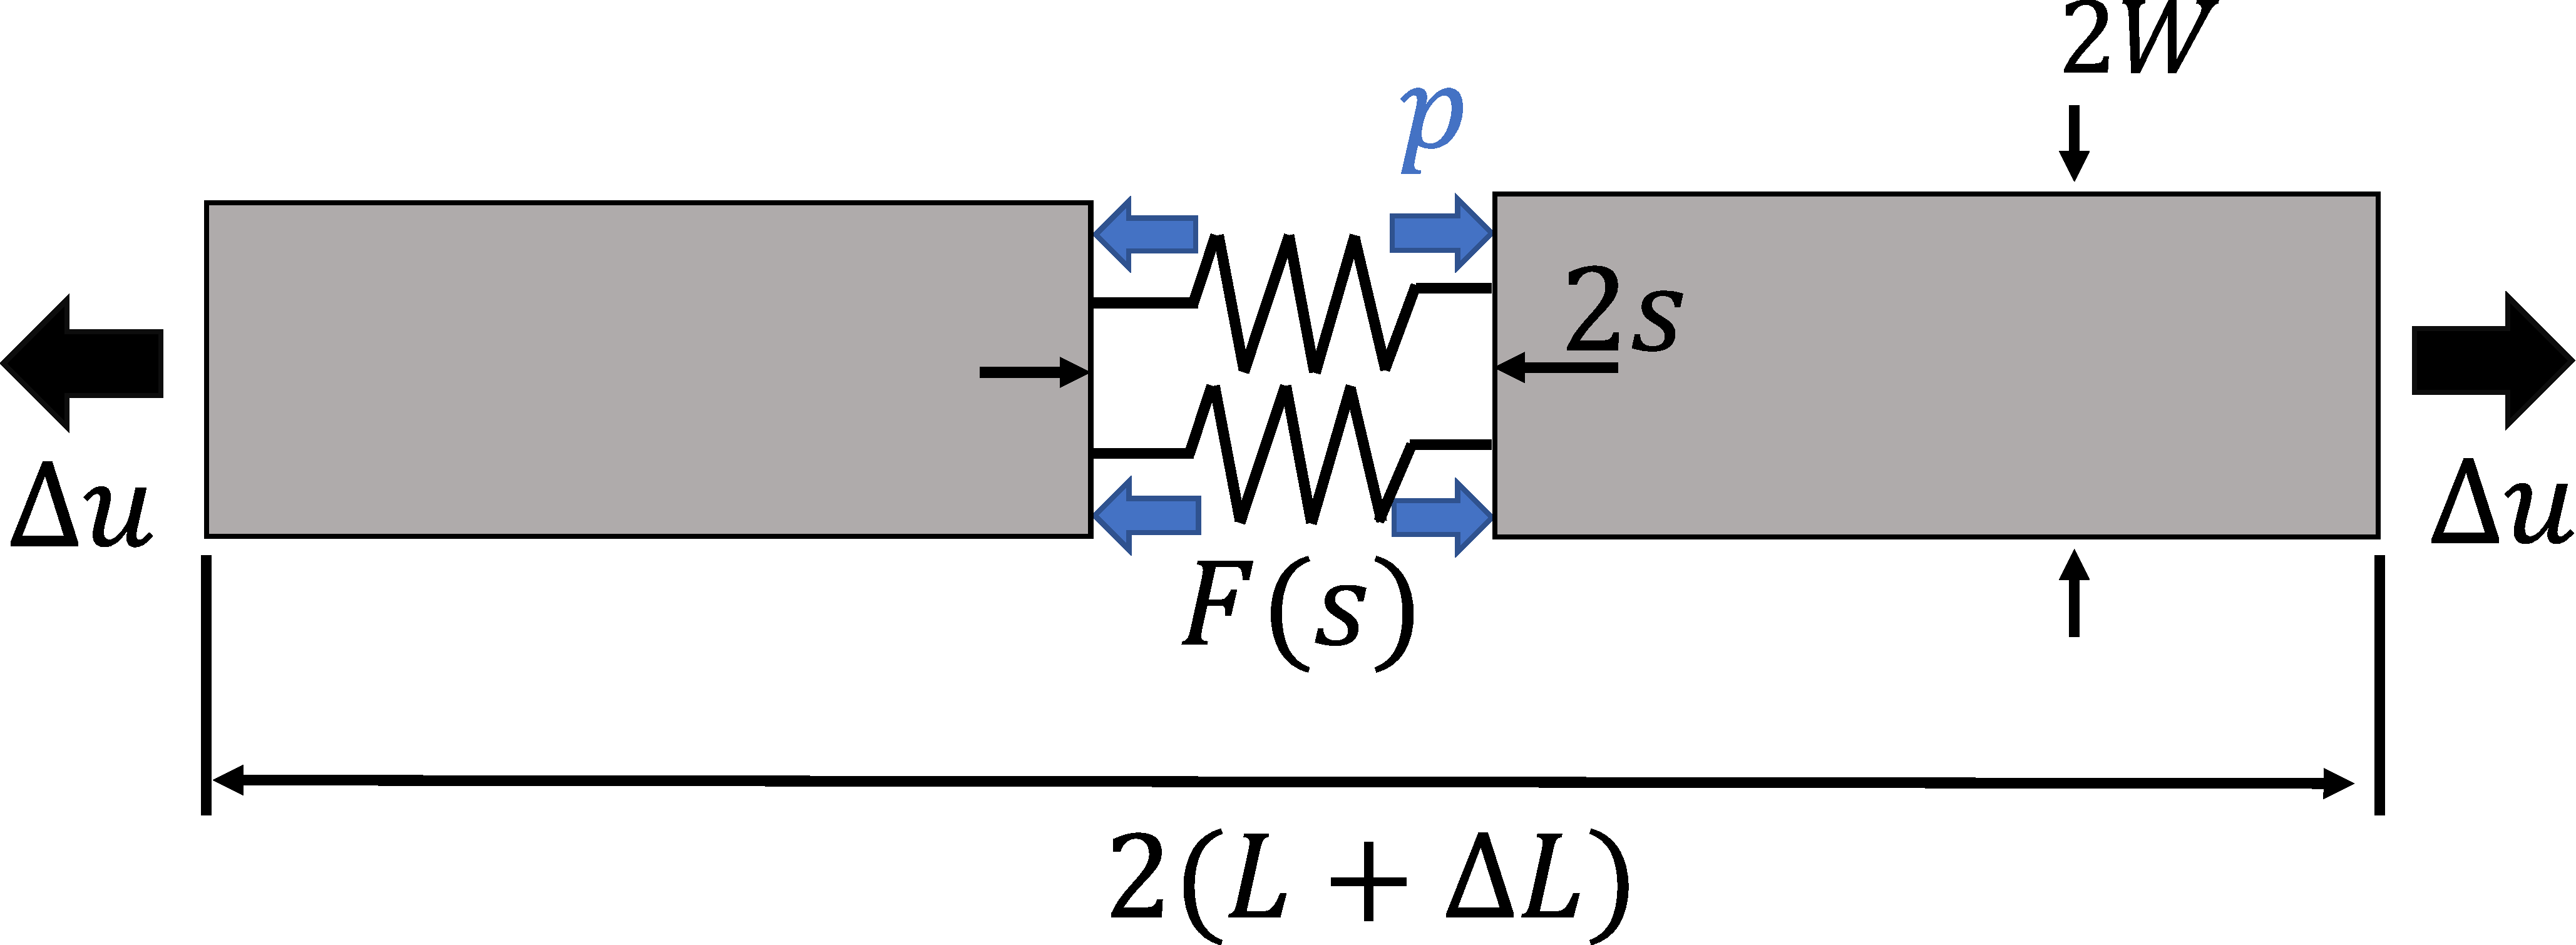
\includegraphics[width=.6\linewidth]{images/traction_separation/uniaxial_cohesive.pdf}
    \caption{Uniaxial cohesive bar.}
    \label{fig:1d_problem_schematic}
\end{figure}

\begin{table}[h]
\centering
\caption{Material properties for uniaxial bar}
\begin{tabular}[t]{lcc}
\hline
&Value &Unit \\
\hline
Young's modulus ($\text{E}$)&4.0$\times10^5$&MPa\\
Poisson's ratio ($\nu$)&0.2&--\\
 Nucleation energy  ($\psi_c$)&5.6$\times10^{-5}$&$\text{mJ mm}^{-3}$\\
Critical fracture energy ($G_c$)&0.12&$\text{mJ mm}^{-2}$\\
%Tensile strength ($\sigma_c$)&3.0&$\text{MPa}$\\
Residual stiffness ($\xi$)&1.0$\times10^{-8}$&--\\
\hline
\end{tabular}
\label{material_properties_p1}
\end{table}%

%\tablefootnote{$\sigma_c$ and $\psi_c$ are related through the expression $2\psi_c = \sigma_c^2(1-\nu^2)/E$ {\color{red} I don't like using a footnote to handle this - let's discuss} }

%{\color{red} Gary pointed out that critical fracture strength and critical fracture energy are somewhat confusing names for $\psi_c$ and $G_c$ So, I looked at what was used in Rudy's 2019 paper, and we have critical fracture energy per volume and per area, which I think is an even more confusing choice. I suggest, for $\psi_c$, "critical energetic strength", "energetic threshold" or "critical fracture energy". For $G_c$, "critical energy release rate" avoids any confusion I believe. }

%physical and numerical setup
The problem consists of a bar under a displacement controlled load in a pressurized chamber, as shown in Figure~\ref{fig:1d_problem_schematic}. The bar is assumed to be made of a linear elastic material that undergoes cohesive fracture, with a traction-separation law $F(s)$.
%A schematic of the problem, after the cracking process begins, is shown in Figure \ref{fig:1d_problem_schematic}. 
The bar has an undeformed length $2L = 400$ mm and width $2W = 2$ mm. The material properties are given in Table \ref{material_properties_p1}. Symmetry boundary conditions are invoked to reduce the computational domain to the top-right quarter of the bar. The applied load is modeled as a displacement boundary condition on the right end of the domain. The mesh consists of rectangular elements of size $h$ along the length direction and size 1 mm in the width direction.
The initial applied displacement increment is $\Delta u = 5\times10^{-4}$ mm. The displacement increment is adaptively refined when convergence is not obtained within a fixed set of iterations.   A more detailed description of the adaptive stepping procedure is provided in \cite{gaston2009moose, permann2020moose, lindsay20222}. 

Damage localization is triggered by introducing an small initial defect ($d = \mathcal{O}(\epsilon)$) on the left side of the domain.  In what follows, results are reported using $\ell = L/20 = 10$ mm and $h = \ell/10 = 1$ mm.  This choice of regularization length and mesh spacing was found to yield spatially-converged results.  
%In addition, all results were obtained using the linear indicator function $I(d) = d$.  
Different values of pressure, ranging from $0$ to $\sigma_c/3$ are considered. 

The problem is simulated using discretized versions of both the \ref{uvc} and \eqref{lvc} formulations.  
%Before investigating the response of various models for this problem, an analysis of convergence with respect to the regularization length $\ell$ and element size $h$ was performed. The analysis indicated that the results were insensitive to $\ell$ and $h$ if $\ell < L/10 = 20$ mm and $h < \ell/5$. The results shown next were obtained with $\ell = L/20 = 10$ mm and $h = \ell/10 = 1$ mm. The linear indicator function $I(d)$ was chosen, but with the \ref{uvc} formulation, the sensitivity to this indicator is minimal.
%reference results
%For comparison, this same problem is also solved with the formulation \eqref{lvc},  which has been employed in several studies, such as \cite{bourdin2012variational, wheeler2014augmented, peco2017influence, wilson2016phase, jiang2022phase}. 
For the indicator function $I(d)$, results are reported for: (1) $I(d) = d$, used for example in \cite{bourdin2012variational}; (2) $I(d) = d^2$, used in \cite{jiang2022phase} and (3) $I(d) = 2d-d^2$, used in \cite{wheeler2014augmented}.
%post-processing details
The effective traction-separation laws extracted from the set of simulations are shown in Figure \ref{fig:traction_separation_results}. To generate these curves, the traction is computed as the internal force measured in the center of the bar. The separation $s$ is the opening of the crack, calculated as $s = -\int\limits_{-\infty}^{\infty}\textbf{u}\cdot\nabla I(d) \text{dx}$ \cite{bourdin2012variational}. 

%which is the left of the computational domain (i.e $t = -R^{\text{left}}_x$ )

\begin{figure}[h]
\centering
\begin{subfigure}{.45\textwidth}
  \centering
  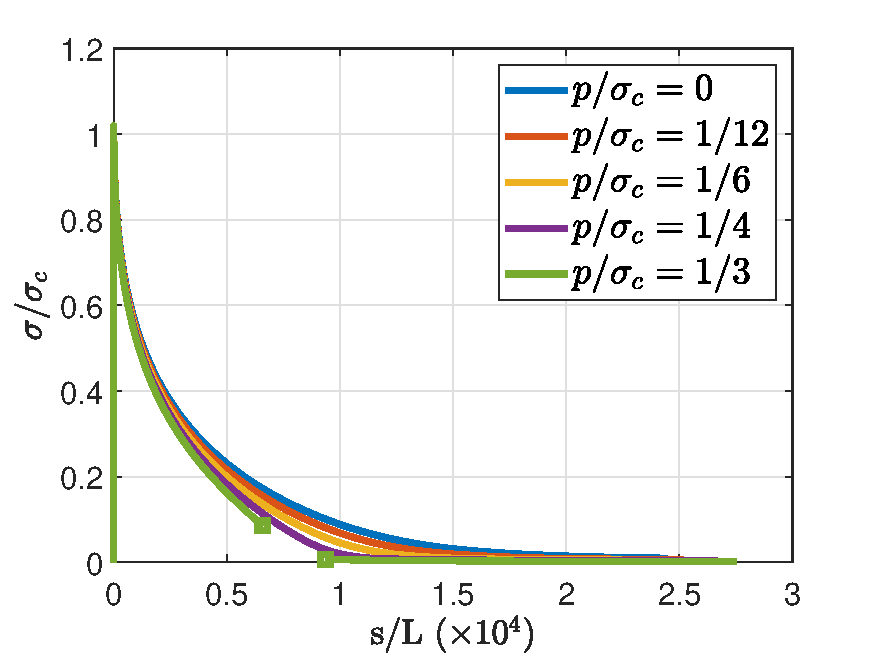
\includegraphics[width=\linewidth]{images/traction_separation/1d_nodash_bourdin_I_d.pdf}
  \caption{}
  \label{fig:traction_separation_bourdin_d}
\end{subfigure}%
\begin{subfigure}{.45\textwidth}
  \centering
  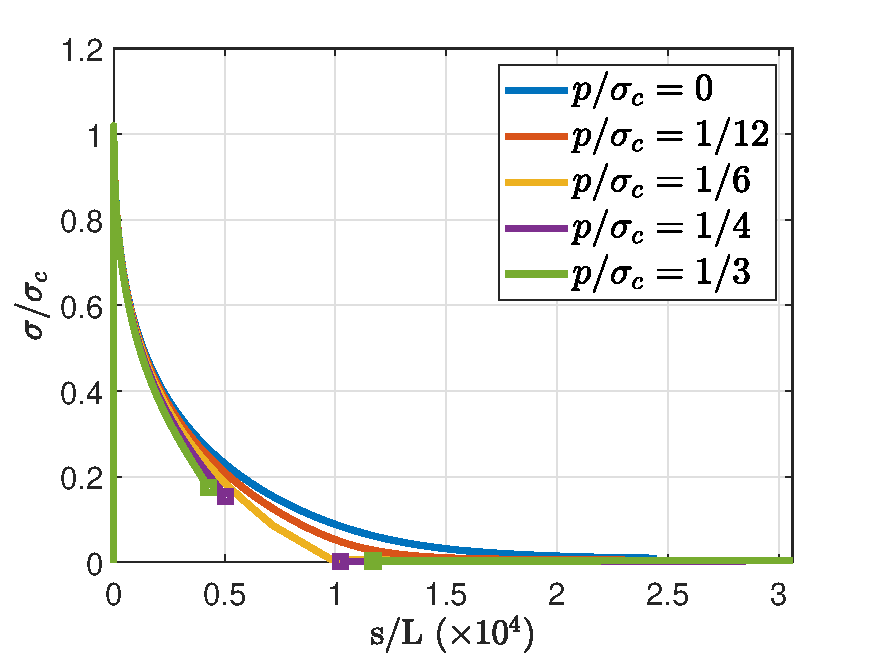
\includegraphics[width=\linewidth]{images/traction_separation/1d_nodash_bourdin_I_d2.pdf}
  \caption{}
  \label{fig:traction_separation_bourdin_d2}
\end{subfigure}%

\bigskip
\begin{subfigure}{.45\textwidth}
  \centering
  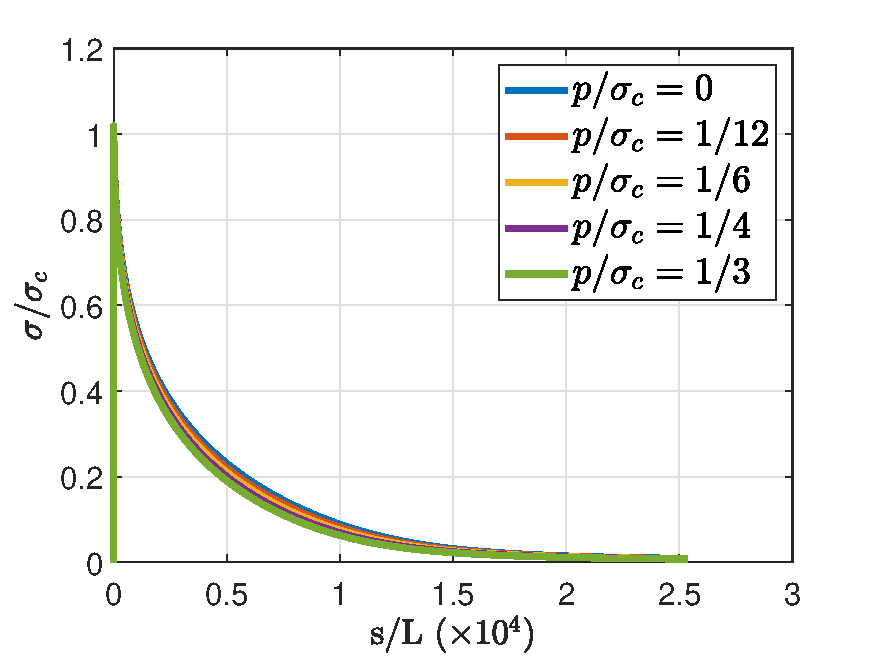
\includegraphics[width=\linewidth]{images/traction_separation/1d_bourdin_I_2d.pdf}
  \caption{}
  \label{fig:traction_separation_bourdin_2d}
\end{subfigure}
\begin{subfigure}{.45\textwidth}
  \centering
  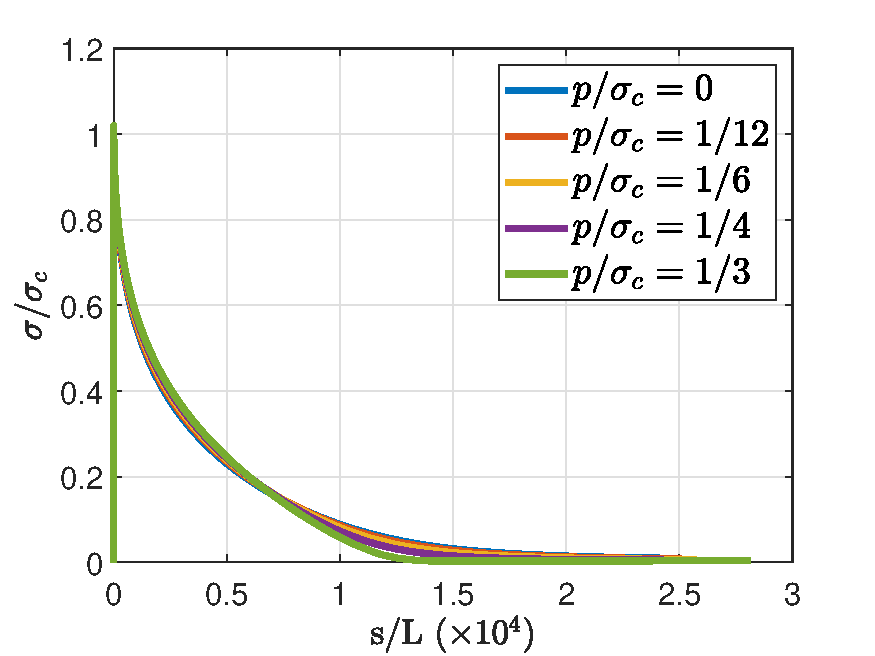
\includegraphics[width=\linewidth]{images/traction_separation/1d_gary_I_d.pdf}
  \caption{}
  \label{fig:traction_separation_gary}
\end{subfigure}
  \caption{Traction-separation curves for pressurized uniaxial cohesive bar problem, obtained with various phase-field models: (a) \eqref{lvc} with linear indicator function; (b) \eqref{lvc} with quadratic indicator function; (c) \eqref{lvc} with $2d-d^2$ indicator function; and (d) Proposed approach \eqref{uvc} with linear indicator function. } 
  \label{fig:traction_separation_results}
\end{figure}

%discussion of results
The results for the various models are shown in Figure \ref{fig:traction_separation_results}, with tractions and pressures normalized by the critical stress $\sigma_c$ from \eqref{eq:sigmacrit-from-psicrit}.
As shown in Figure \ref{fig:traction_separation_results}, the proposed model \eqref{uvc} exhibits minimal sensitivity to the pressure magnitude in the traction-separation behavior.  
By contrast, with the \eqref{lvc} formulation, only the case with $I(d) = 2d - d^2$ exhibits comparable results. In the other two cases (Figures \ref{fig:traction_separation_bourdin_d} and \ref{fig:traction_separation_bourdin_d2}), the apparent traction-separation law shows a spurious dependence to the applied pressure. This is evident in the variations in the results as well as the presence of jumps in the aperture at sufficiently high pressures. The latter occur due to an instability of the partially damaged solutions as $d$ approaches 1. More precisely, shortly after the damage at the center of the bar reaches $d\approx 0.8$, it jumps to $d= 1$, which in turns lead to a jump in the aperture.  
 This jump is indicated via the squares that appear on selected curves in Figures \ref{fig:traction_separation_bourdin_d} and \ref{fig:traction_separation_bourdin_d2}. The use of smaller displacement increments was not observed to significantly impact these results.   By contrast, such instabilities were not observed for the simulations reported in  Figures \ref{fig:traction_separation_bourdin_2d} and \ref{fig:traction_separation_gary}.

%As a result, the traction-separation laws exhibit the gaps at the points indicated by the solid squares. This phenomenon is not observed in the cases depicted in Figures \ref{fig:traction_separation_bourdin_2d} and \ref{fig:traction_separation_gary}.

% This example is designed to verify the cohesive response of an uniaxial specimen in the presence of a pressure. The setup consists of a bar, under a displacement controlled load, in a pressurized chamber. The bar is assumed to be made of a linear elastic material that undergoes cohesive fracture, with a traction-separation law $F(s)$. A schematic of the problem, after the cracking process begin, is shown in Figure \ref{fig:1d_problem_schematic}.

% The possibility of retrieving a cohesive fracture behavior with a phase-field model was established for traction-free cracks in \cite{lorentz2011convergence}, with the use of the degradation function \eqref{cohesive_degradation}. However, up to this point, the influence of a pressure load in this scenario has not been investigated. So, to shed light in this question, the model in this example combines the use of the degradation function \eqref{cohesive_degradation} with the two formulations for incorporating pressure, described in Section \ref{sec:model}.

% First, the pressure load is introduced using the formulation \eqref{lvc}, which has been employed in several studies, such as \cite{bourdin2012variational, wheeler2014augmented, peco2017influence, wilson2016phase, jiang2022phase}. This formulation requires the use of an indicator function $I(d)$, that identify the regions where the pressure load is applied. The cases $I(d) = d$, used for example in \cite{bourdin2012variational}, $I(d) = d^2$, which appeared in \cite{jiang2022phase} and $I(d) = 2d-d^2$, chosen in \cite{wheeler2014augmented} are considered.

% Then, the results are then compared with the ones obtained using the proposed formulation \eqref{uvc}, with the simplest indicator function $I(d) = d$. 

% To model the cohesive fracture behavior, the phase-field model uses the degradation function \eqref{cohesive_degradation}. In the absence of pressure, it is shown in \cite{lorentz2011convergence} that this choice allows the phase-field model to represent, as $\ell \rightarrow 0$, the physics of 

% As discussed in Section \ref{sec:model} (subsection 2.2), it was shown in \cite{lorentz2011convergence, lorentz2011gradient, geelen2019phase, wu2017unified} that, by using the degradation function \eqref{cohesive_degradation} one can approximate certain families of cohesive responses with a phase-field model of fracture. The additional assumption that $F(s)$ is a member of one of these families is then necessary. CLARIFY THAT (31) IS USED WITH NO SPLIT.

% The first numerical example consists of a bar, under a displacement controlled load, in a pressurized environment. The bar is assumed to be made of a linear elastic material, that undergoes cohesive fracture, with a traction-separation law $F(s)$. A schematic of the problem, after the cracking process begin, is shown in Figure \ref{fig:1d_problem_schematic}. The bar has length $2L = 400$ mm and width $2W = 2$ mm. The material properties are given in Table \ref{material_properties_p1}. 

% {\color{blue} Quick analysis of the problem

% \begin{equation}\tag{Total deformation}
%     L\dfrac{\sigma}{E} + \dfrac{s}{2} = L + \Delta u
% \end{equation}

% \begin{equation}\tag{Force balance}
%     \sigma = -p + F(s)
% \end{equation}

% \begin{equation}\tag{Nonlinear equation for s}
%     F(s) + \dfrac{sE}{2L} = E\left( 1 + \dfrac{\Delta u}{L} \right) + p
% \end{equation}

% }

% As discussed in Section \ref{sec:model} (subsection 2.2), it was shown in \cite{lorentz2011convergence, lorentz2011gradient, geelen2019phase, wu2017unified} that, by using the degradation function \eqref{cohesive_degradation} one can approximate certain families of cohesive responses with a phase-field model of fracture. The additional assumption that $F(s)$ is a member of one of these families is then necessary. CLARIFY THAT (31) IS USED WITH NO SPLIT.

% The value of this example resides on the fact that the traction-separation law $F(s)$ is an intrinsic property of the material, and therefore, should be independent of any applied loads and pressures. {\color{red}To the author's knowledge, although phase-field models for quasi-brittle fracture have been used to simulate pressure-driven cracks in \cite{jiang2022phase, li2022hydro}, this simple verification has not been performed.}

% \begin{figure}[!htbp]
% \centering
% \begin{minipage}{.48\textwidth}
%   \centering
%   \includegraphics[width=\linewidth]{images/gary_several_ps.png}
%   \caption{Traction-separation response with proposed model.}
%   \label{fig:1d_bar_gary}
% \end{minipage}%
% \hfill
% \begin{minipage}{.48\textwidth}
%   \centering
%   \includegraphics[width=\linewidth]{images/bourdin_several_ps.png}
%   \caption{Traction-separation response with existing models.}
%   \label{fig:1d_bar_bourdin}
% \end{minipage}
% \end{figure}

% \begin{figure}[h]
% % \centering
% \begin{subfigure}{.33\textwidth}
%   \centering
%   \includegraphics[width=\linewidth]{images/traction_separation/traction_separation_bourdin.pdf}
%   \caption{}
%   \label{fig:traction_separation_quadratic}
% \end{subfigure}%
% \begin{subfigure}{.33\textwidth}
%   \centering
%   \includegraphics[width=\linewidth]{images/traction_separation/traction_separation_quadratic.pdf}
%   \caption{}
%   \label{fig:traction_separation_bourdin}
% \end{subfigure}%
% \begin{subfigure}{.33\textwidth}
%   \centering
%   \includegraphics[width=\linewidth]{images/traction_separation/traction_separation_gary.pdf}
%   \caption{}
%   \label{fig:traction_separation_gary}
% \end{subfigure}
%   \caption{(a) Quadratic indicator function; (b) Linear indicator function; and (c) Proposed approach. } 
%   \label{fig:traction_separation_results}
% \end{figure}



%Gamma convergence figure - could add 3 of these
% \begin{figure}[h]
%     \centering
%     \includegraphics[width=.6\linewidth]{images/traction_separation/gamma_convergence_gary.pdf}
%     \caption{Verify reg. length independence, p = 0.5MPa.}
%     \label{fig:gamma_convergence}
% \end{figure}
%\FloatBarrier
\subsection{Crack nucleation from a pressurized hole}

Consider a square plate of dimensions $L \times L$, with a circular hole in the center subjected to an internal pressure $p$, as shown in Figure \ref{fig:cavity_schematic}. This problem is motivated by oil and gas wellbore systems.   Far field stresses $\sigma_V$ and $\sigma_H$ are applied as tractions on the boundaries as shown. 
%This setup can be viewed, for example, as the cross-section of an oil and gas wellbore. 
The pressure is increased until it reaches a ``breakdown pressure" $p_b$. When that happens, cracks initiate in the direction parallel to the maximum \textit{in-situ} stress. Assuming $\sigma_H > \sigma_V$, this is expected to occur along a horizontal axis passing through the center of the hole.  In this work, the pressure in the hole is assumed to follow the crack faces as the fracture grows into the interior of the domain.  

\begin{figure}[h]
% \centering
\begin{subfigure}{.49\textwidth}
  \centering
  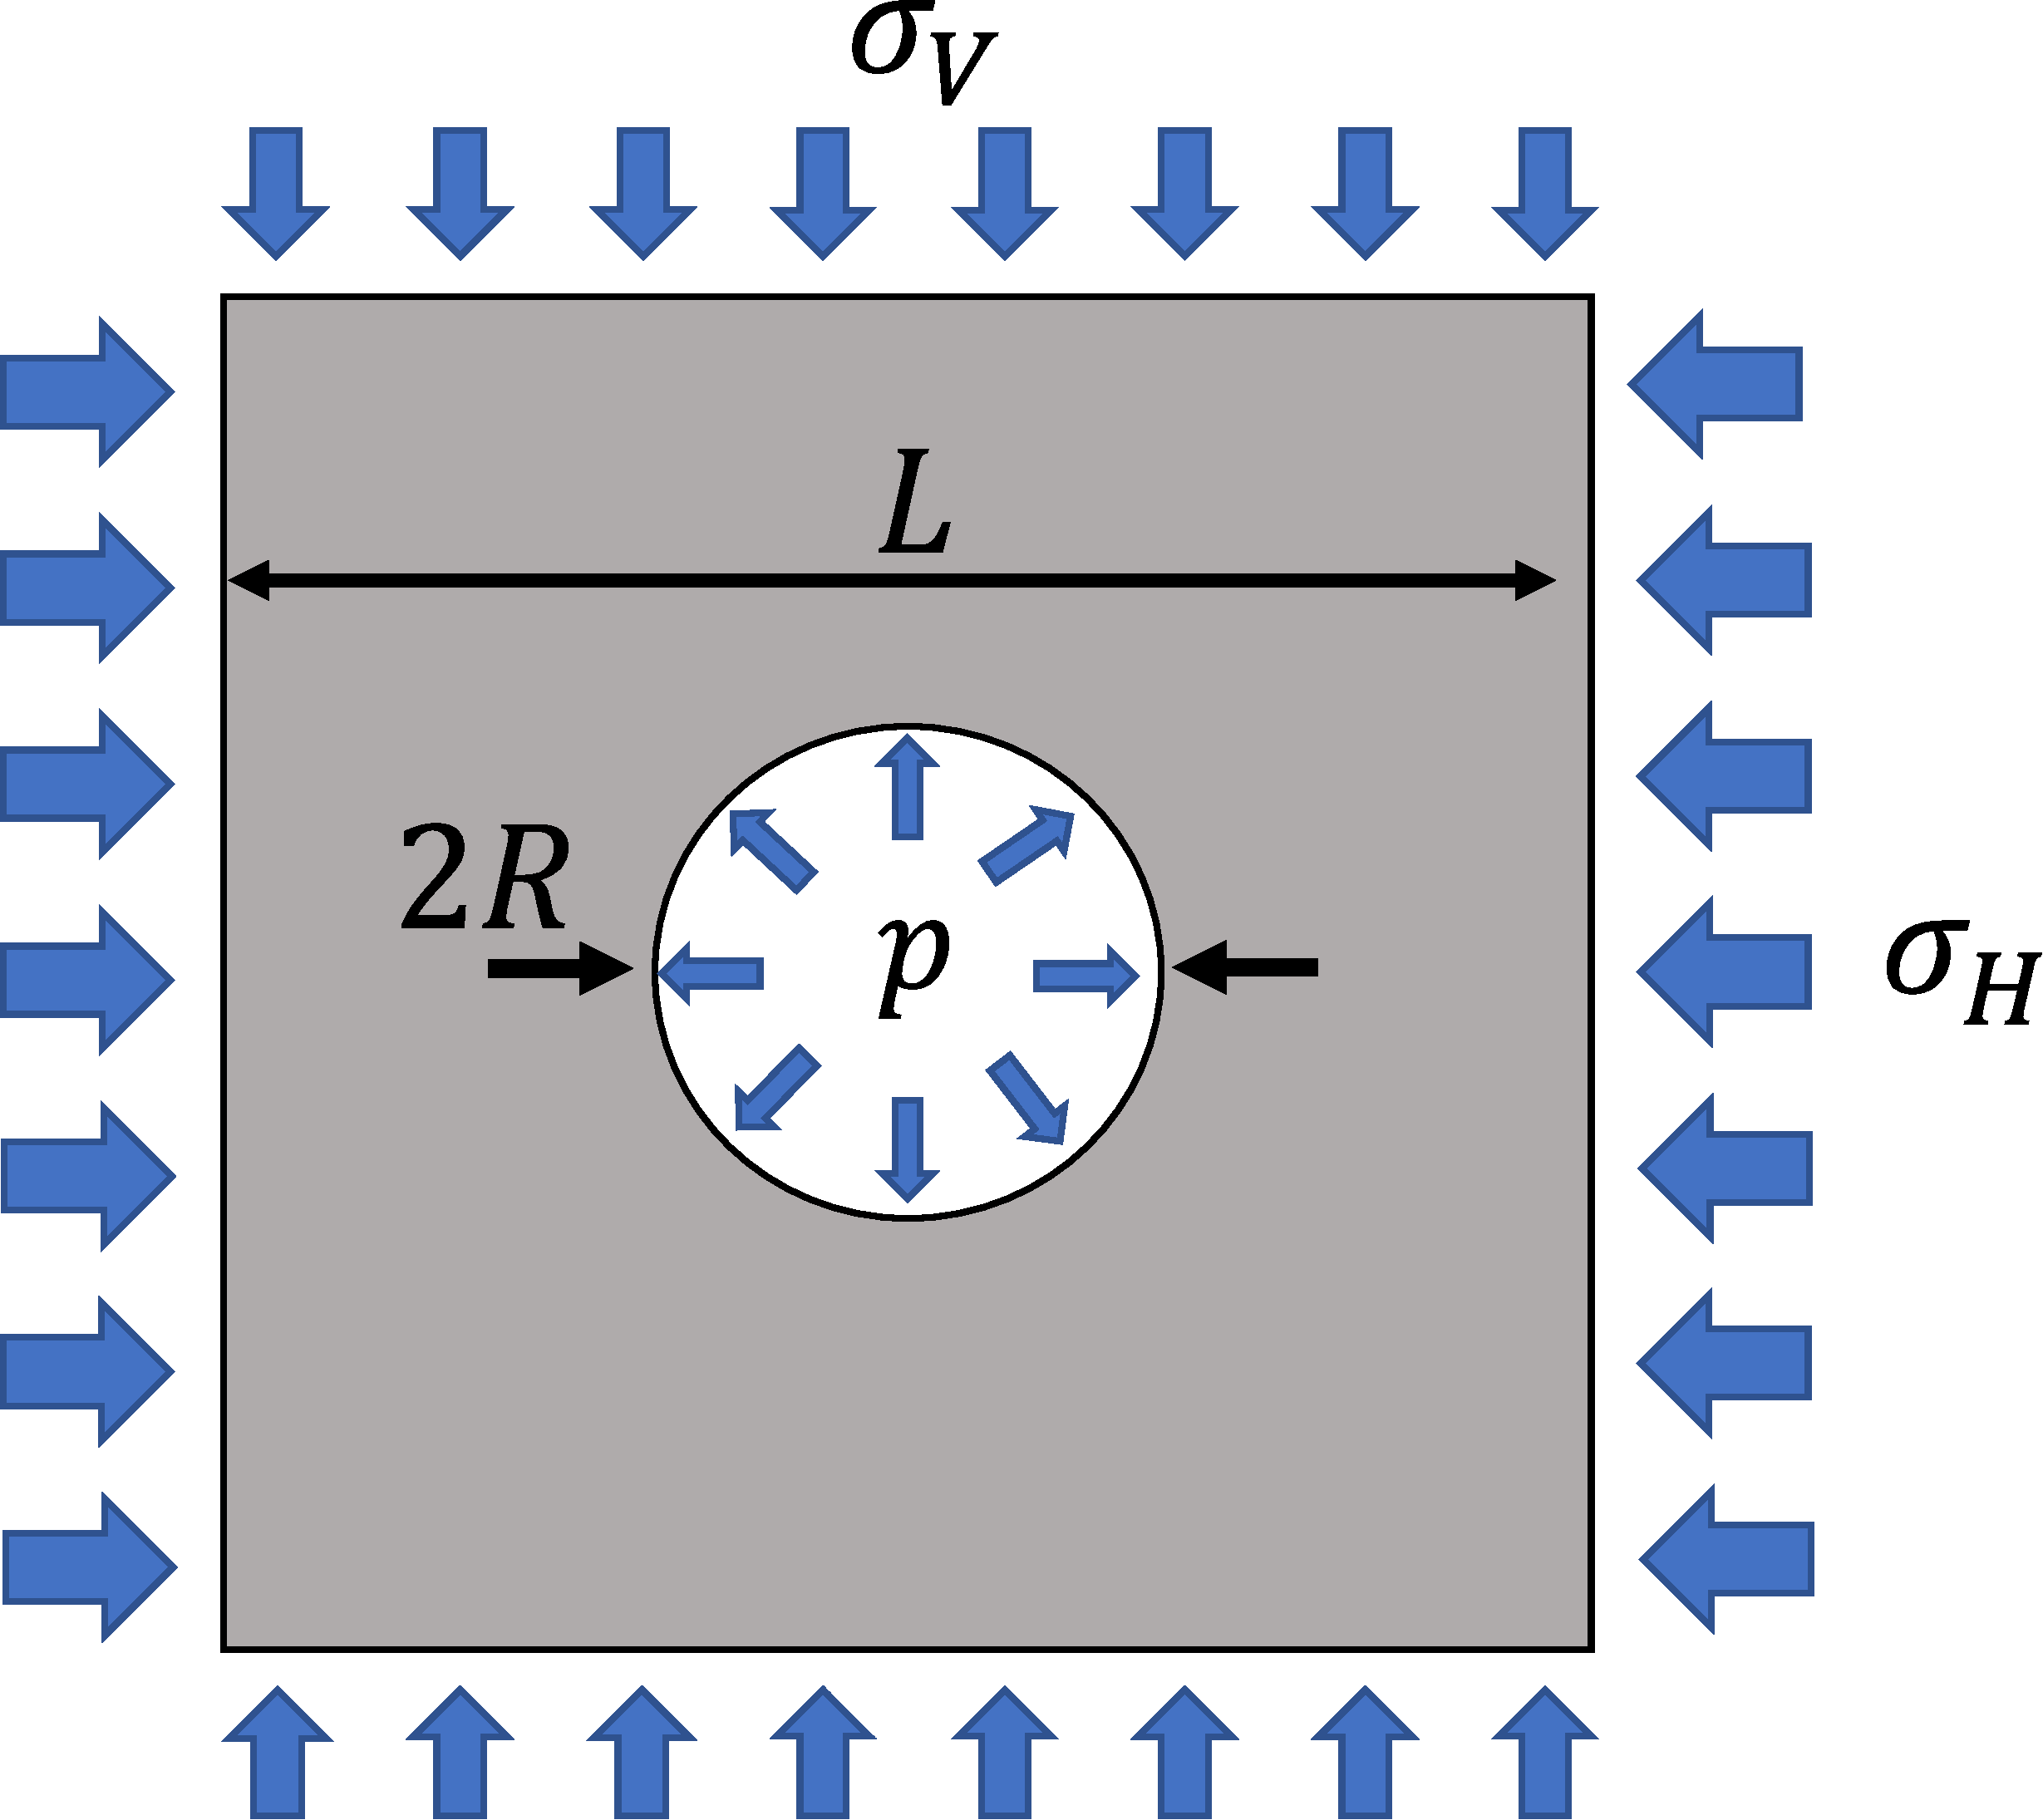
\includegraphics[width=0.8\linewidth]{images/2d_nucleation/cavity_schematic.pdf}
  \caption{}
  \label{fig:cavity_schematic}
\end{subfigure}%
\begin{subfigure}{.49\textwidth}
  \centering
  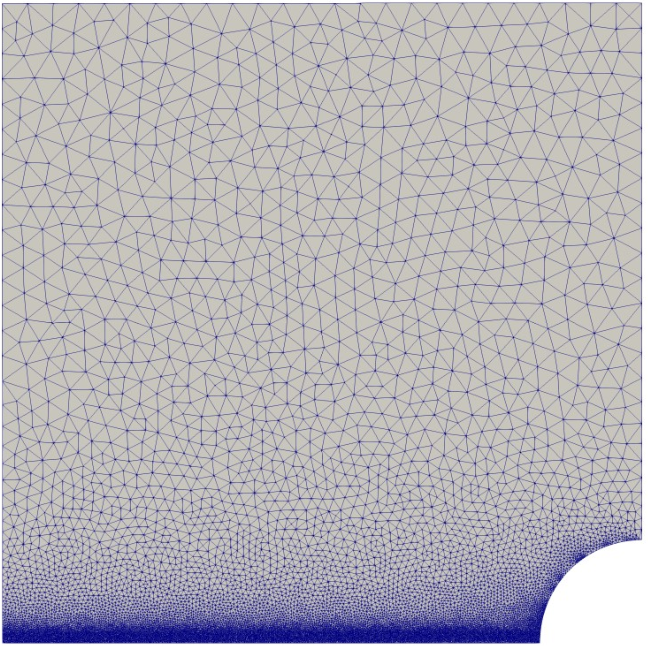
\includegraphics[width=0.71\linewidth]{images/2d_nucleation/quarter_mesh.pdf}
  \caption{}
  \label{fig:quarter_mesh}
\end{subfigure}%
  \caption{(a) Problem schematic; (b) Mesh used in the computations, exploiting symmetry. } 
  \label{fig:initiation_problem_setup}
\end{figure}

\begin{table}[h]
\centering
\caption{Material properties, geometric parameters and applied loads for crack initiation problem}
\begin{tabular}[t]{lcc}
\hline
&Value &Unit \\
\hline
Young's modulus ($\text{E}$)&19.0$\times10^3$&MPa\\
Poisson's ratio ($\nu$)&0.2&--\\
Nucleation energy ($\psi_c$)&7.96$\times10^{-4}$&$\text{mJ mm}^{-3}$\\
Critical fracture energy  ($G_c$)&7.70$\times10^{-2}$&$\text{mJ mm}^{-2}$\\
Cavity radius ($R$)&400&mm\\
Specimen length ($L$)&5.0$\times10^{3}$&mm\\
Horizontal stress ($\sigma_H$)&5.0&MPa\\
Vertical stress ($\sigma_V$)&2.5&MPa\\
\hline
\end{tabular}
\label{material_properties_initiation}
\end{table}

%The propagation of the fracture after the breakdown pressure is reached depends on the nature of the applied load. If one assumes that the pressure applied to the cavity follows the fracture as it grows (for example, if the cavity is filled by a high pressure gas), then crack propagation will be unstable and result in complete failure of the specimen. However, if the cracks are assumed to be traction-free, it is possible to obtain stable growth, and total failure of the specimen will occur only if the applied pressure is further increased. This latter scenario has been investigated using a phase-field model of fracture, in the work of Tanné \cite{tanne2017variational}. In this work, the former case is considered.

The material properties selected for this problem, along with the dimensions and loading parameters are listed in Table \ref{material_properties_initiation}.  The material properties are taken to be representative of a Bebertal sandstone, as inspired by the experiments of \cite{stoeckhert2015fracture}.
%In {\color{purple}terms of material properties, a Bebertal sandstone is used,} following the experiments of \cite{stoeckhert2015fracture}. They are listed, alongside with the geometric parameters and applied loads in Table \ref{material_properties_initiation}. 
The symmetry of the problem is exploited to reduce the computational domain to the top-left quarter.  An unstructured triangular mesh is used, with local refinement along the $x$-axis, as shown in Figure \ref{fig:quarter_mesh}. The element size in the refined area is $10$mm, whereas the phase-field regularization length is $\ell = 40$mm. For the results reported in this section, the phase-field model employs the cohesive formulation\cite{lorentz2011convergence, geelen2019phase} using the degradation function \eqref{cohesive_degradation} and the spectral split of  \cite{miehe2010phase}.  

%, that uses the degradation function \eqref{cohesive_degradation} is again employed.  As the applied loads give rise to considerable compression in the domain, the split proposed in \cite{miehe2010phase} is used in the model.  

%, as it provides a bound for crack initiation that is independent of the regularization length. {\color{purple}Since the load has a large compressive part, a decomposition of the strain is needed.} The spectral split proposed in \cite{miehe2010phase} is then used.

Intuitively, the magnitude of the pressure load required to initiate fracture in this problem is expected to be independent of whether or not the pressure follows the crack evolution. After initiation, the pressure effects become important and the fracture propagates unstably. Due to this unstable behavior, it is very difficult to numerically capture the crack path after the pressure $p_b$ is reached. In order to have a glimpse into what this path looks like, a viscous term $\eta \dot d$ is added to the phase-field equation, as in \cite{miehe2010phase}, with $\eta = 10^{-3}\  \text{mJ}\cdot\text{mm}^{-3}\cdot$s. 

It bears emphasis that the equations \eqref{disp equation} and \eqref{damage equation ch2} indicate that, in the absence of any damage, the proposed model for pressurized cracks reduces to the standard phase-field fracture model for traction-free cracks. Therefore, one should expect the proposed model to capture fracture initiation properly in this scenario. On the other hand, for the \eqref{lvc} formulation, this only occurs if the indicator function satisfies $I'(0) = 0$. Among the many works which use the \eqref{lvc} formulation, only a few such as \cite{jiang2022phase, peco2017influence} used an indicator function satisfying this condition. In \cite{jiang2022phase}, the authors were indeed able to predict fracture initiation from pressurized holes. To highlight the implications of having $I'(0) \neq 0$ in the model \eqref{lvc}, the results for this problem will also be presented using the  \eqref{lvc} formulation with the indicator function $I(d) = d$.

% WHICH INDICATOR FUNCTION? HOW TO SEPARATE THE I(d) = d2 CASE
%  Although it leads to the not so interesting case of unstable propagation, it illustrates a limitation of  the formulation \eqref{lvc}, which, in these conditions, will predict spurious damage growth in the domain boundaries. That happens due to the presence of the term $p\nabla\cdot u$ in equation \eqref{wet damage equation box 2}, even when the material is intact. This issue is circumvented when the formulation \eqref{uvc} is applied since no modification to the evolution equation for damage is made. 

% Since the fracture propagates unstably, it is very difficult to numerically capture its path after the pressure $p_b$ is reached. In order to have a glimpse on what the path looks like, a viscous term $\eta \dot d$ is added to the phase-field equation, as in \cite{miehe2010phase}, with $\eta = 10^{-3}\  $MPa$\cdot$s.

%For an infinite plate, the breakdown pressure can be estimated by the Hubbert and Willis formula \cite{hubbert1957mechanics}, which assumes that failure occurs when the maximum hoop stress in the cavity reaches the tensile strength $\sigma_c$. However, due to the finite size of the computational domain, a more precise verification consists in comparing the maximum value of $\sigma_{\theta\theta}$ prior to crack nucleation to $\sigma_c$, from \eqref{eq:sigmacrit-from-psicrit}.  

The final damage patterns obtained using the \eqref{uvc} formulation and the \eqref{lvc} formulation  are shown in Figure \ref{fig:damage_profiles}. With the \eqref{uvc} formulation, damage localizes along the midplane when the hoop stress is approximately 85\% of $\sigma_c$.  This is not unexpected, as the expression \eqref{eq:sigmacrit-from-psicrit} is based on a one-dimensional state of stress and strain which differs significantly from the state near the corner of the hole.    The same comparison is not performed for the simulation using the model \eqref{lvc}, since damage forms only on the boundary in the first steps leading to spurious rigid body motion. 

% However, since in most application cases the pressure load comes from some invading fluid, the viscosity of this fluid will stabilize the fracture evolution and this additional term will not be necessary.

%Table \ref{results_initiation} compares the prescribed values of $\sigma_c$ and $\psi_c$ with those obtained in the simulation using the proposed model. The simulation values are computed at the onset of damage initiation, in the location where the damage begins. {\color{red}(i.e we look at the first point that sees $d > 0$ and take its $\Psi_e$ and $\sigma_c$ at that instant. )} The same comparison is not performed for the simulation using the model \eqref{lvc}, since damage forms only on the boundary in the first steps leading to spurious rigid body motion. The final damage profiles are shown in Figure \ref{fig:damage_profiles}. 

%\begin{table}[ht]
%\centering
%\caption{Comparison of results}
%\begin{tabular}[t]{lcccc}
%\hline
%&$\sigma_c$(Simulation) & $\sigma_c$(Prescribed) & $\psi_c$(Simulation) & $\psi_c$(Prescribed) \\
%\hline
%\eqref{uvc} formulation & 4.73 & 5.60 & 7.98e-4 & 7.96e-4\\
%\hline
%\end{tabular}
%\label{results_initiation}
%\end{table}

\begin{figure}[h]
% \centering
\begin{subfigure}{.49\textwidth}
  \centering
  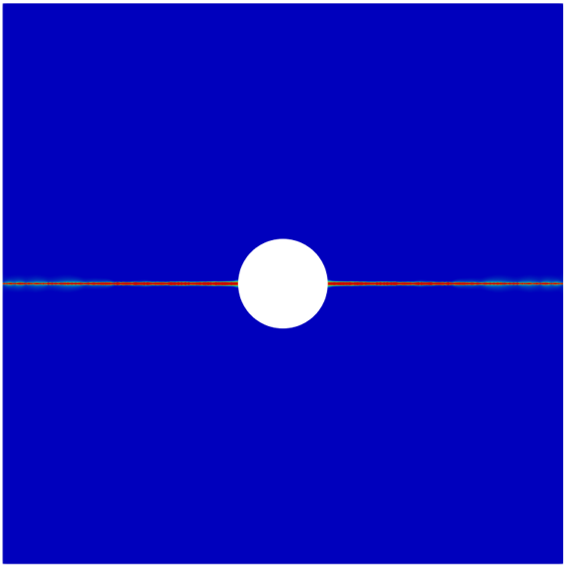
\includegraphics[width=0.7\linewidth]{images/2d_nucleation/gary_crack.png}
  \caption{}
  \label{fig:damage_profile_gary}
\end{subfigure}%
\begin{subfigure}{.49\textwidth}
  \centering
  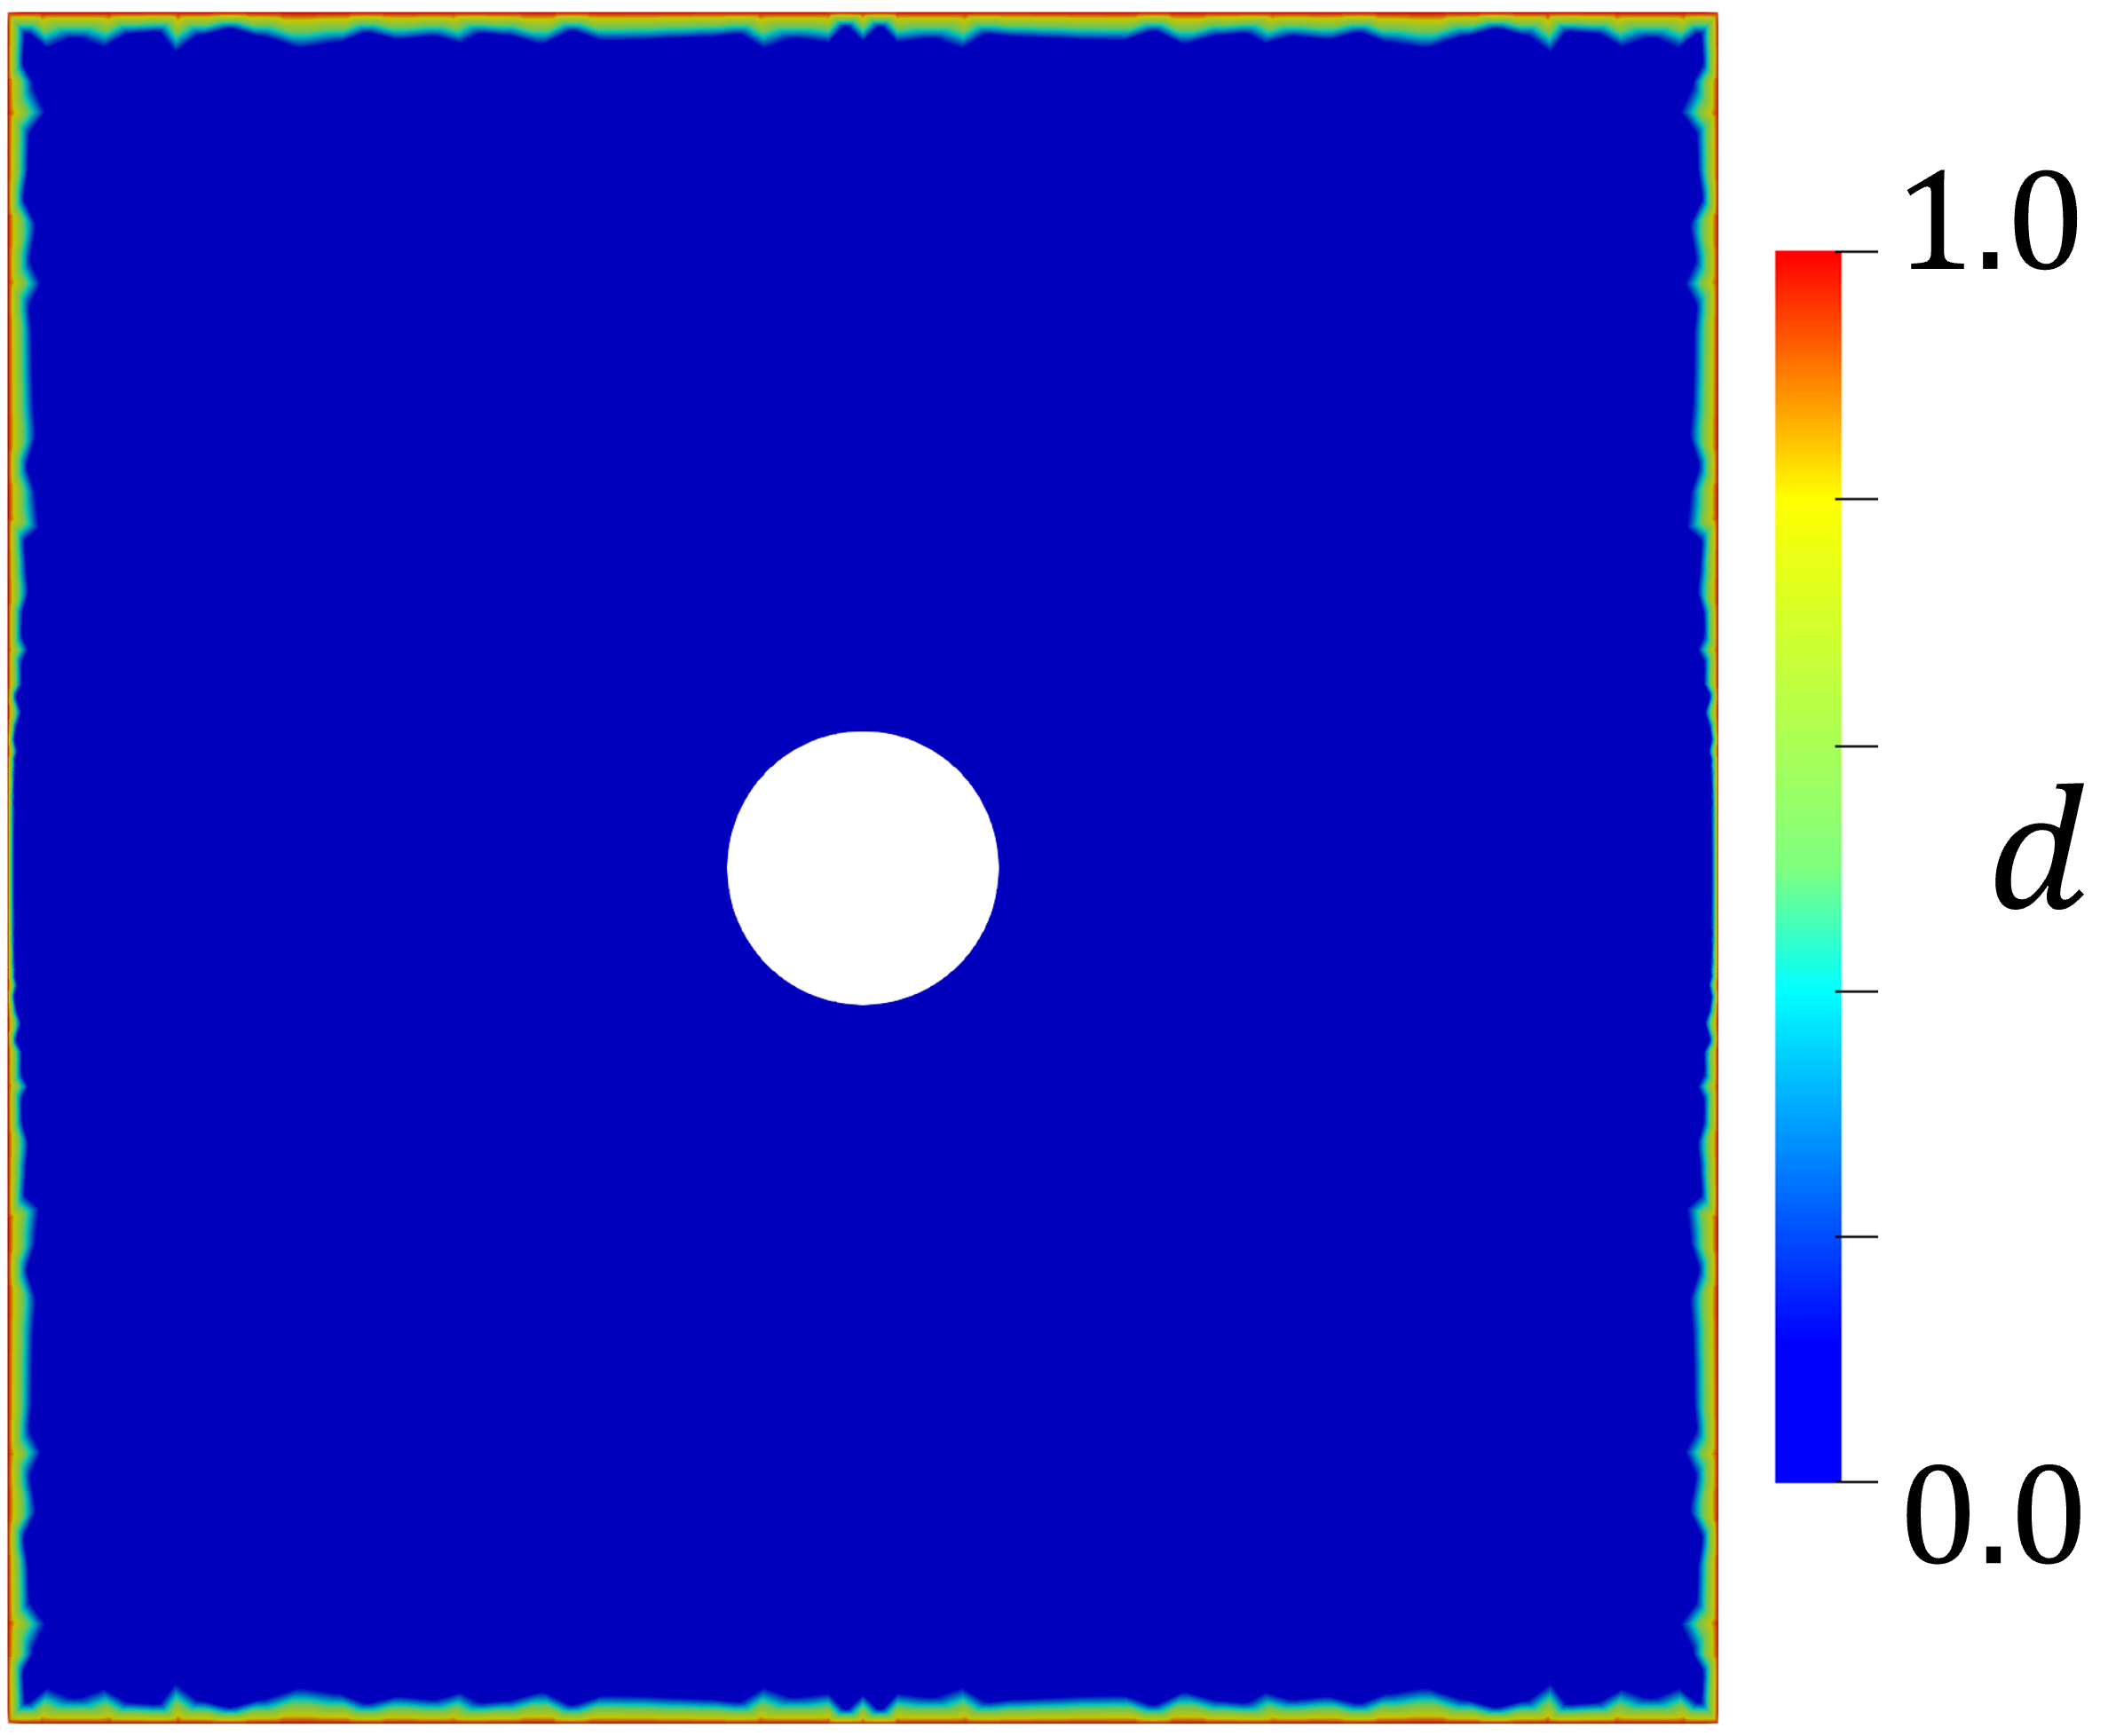
\includegraphics[width=0.86\linewidth]{images/2d_nucleation/bourdin_crack.png}
  \caption{}
  \label{fig:damage_profile_bourdin}
\end{subfigure}%
  \caption{(a) Final crack pattern using proposed model; (b) Damage field using the model from \cite{bourdin2012variational}. } 
  \label{fig:damage_profiles}
\end{figure}

The main takeaway is that the proposed model \eqref{uvc} allows one to study crack nucleation and subsequent propagation under a pressure load, whereas formulation \eqref{lvc} leads to spurious damage formation if $I'(0) \neq 0$. The presence of the term $p\nabla \cdot \textbf{u}I'(d)$ in the damage equation \eqref{wet damage equation box2} drives crack formation in areas which are not stressed. For this specific problem, this issue can be circumvented using for example $I(d) = d^2$, as shown in \cite{jiang2022phase}, but this option introduces a spurious dependence of the cohesive response of the material on the applied pressure, as indicated in the last section (Figure \ref{fig:traction_separation_bourdin_d2}).

%Although the proposed formulation \eqref{uvc} displays a good qualitative comparison with the theory in this example, the error in the predicted $\sigma_c$ must also be explained. It comes from the fact that, in the cohesive phase-field formulation used herein, damage initiation is governed by a strain energy envelope $\psi_e^+(\bs\epsilon(\textbf{u}))\le\psi_c$. In this two-dimensional setting, and using the spectral split to compute $\psi_e^+$, the relationship used to define $\sigma_c = \psi_c/2E$ does not hold. Since the cohesive model relies $\psi_c$ as a bound for damage initiation, the comparison between the simulated and prescribed values for this quantity will be much better than the same comparison for $\sigma_c$ in two or three dimensions. The general applicability of the strain energy as a bound for fracture initiation is debatable in certain circumstances, such as in cases with nearly incompressible materials \cite{kumar2020revisiting}. In future work, phase-field formulations specifically tailored to match experimentally-tested strength envelopes, such as \cite{kumar2020revisiting, de2021nucleation, navidtehrani2022general} will be investigated.

% The direct comparison between \eqref{hubbert_and_willis} and numerical simulations with phase-field requires further explanation. Two key assumptions behind \eqref{hubbert_and_willis} are that crack initiation is governed by the uniaxial tensile strength $T$ and that the domain is infinite. Both of these are not satisfied in the numerical simulations. The domain is finite, with $L = 5$ m and crack initiation is governed by the strain energy envelope, with a threshold $\psi_c$. In a uniaxial case, this threshold is equivalent to a tensile strength of $\sigma_c = \sqrt{2E'\psi_c}$, and this value is calibrated to match $T$. However, the stress state in the cavity problem is not uniaxial, and therefore, all components of the stress will play a role in crack initiation. Due to these differences, the discrepancy between the values of $p_b$ coming from \eqref{hubbert_and_willis} and the model \eqref{u_equation}-\eqref{d_equation} are not concerning. When the critical strain energy measured in the simulation is compared with what is prescribed as a material parameter, the discrepancy is minimal.  



% In our second example, we will consider the case of a plate with a hole, in which the whole is uniformly pressurized on its contour. For example, this scenario could represent a cross section of a pipe or a pressure vessel. If cracks start to form in the plate, the high-pressure gas will occupy the aperture space and apply pressure in the crack faces, therefore, it is important to account for these loads. 

% This problem is particularly interesting because it involves two different modellings of the same pressure load. When the pressure is acting in the walls of the hole, it is modeled with Neumann boundary conditions, whereas as soon as cracks start to form, it has to be account also in these newly formed surfaces, with a phase-field regularization. 

% To correctly predict crack initiation, the phase-field regularization of the pressure load must be designed so that, in the early stages, before any damage kicks in, it effectively recover the underlying phase-field model without any pressure effects, even though there are terms involving the pressure in the governing equations. This only happens if all terms involving the pressure are weighted by the damage variable. 

% If we observe the governing equations for our proposed model (\ref{u_equation} - \ref{d_equation}), that condition is satisfied. Whereas, for the system (\ref{u_equation_bourdin} - \ref{d_equation_bourdin}), the presence of the term $p\nabla \cdot u$ violates it. The main consequence, as we will see, is that damage initiation will happen at much lower loading conditions and in areas which are not at the highest stresses.

% DISCUSS REGULARIZATION LENGTH AND ELEMENT SIZE

% $\ell = 0.04;\ h = 0.01$

% ADD SCHEMATIC OF THIS PROBLEM

% \begin{figure}[!htbp]
% \centering
% \includegraphics[width=0.4\linewidth]{images/2d_nucleation/2d_initiation_schematic.pdf}
% \caption{Problem description.}
% \label{fig:p2_schematic}
% \end{figure}

% ADD RESULTS OF THIS PROBLEM

% \begin{figure}[!htbp]
% \centering
% \includegraphics[width=0.7\linewidth]{images/p_results_plot.png}
% \caption{Comparison of critical loads.}
% \label{fig:p2_schematic}
% \end{figure}

% \begin{figure}[!htbp]
% \centering
% \includegraphics[width=\linewidth]{images/p2_results.png}
% \caption{Crack patterns.}
% \label{fig:p2_schematic}
% \end{figure}

% These results highlight what is arguably the most remarkable advantage of our proposed model. As we can see, the cracks nucleate exactly at the stress concentrations, and exactly when the critical stress, which is an material property in the cohesive phase-field model is reached, even though the original equations are modified to account for pressure loads in the cracks. That is definitely a desirable outcome, since before the onset of damage, we expect this system to behave exactly as a system that does not account for pressure inside the cracks.

% On the other hand, using a model like (\ref{u_equation_bourdin} - \ref{d_equation_bourdin}), leads to crack nucleation at a location which doesn't have the highest stresses. This is a consequence of the term $p\nabla \cdot u$ acting as a driving force to damage formation, even though all the pressure effects prior to the onset of damage are already being accounted for in the Neumann boundary conditions. Worse than that, the threshold for damage initiation is well below the critical stress prescribed by the cohesive model, which definitely does not agree with the assumption that the pressure effects only start after damage initiates.

\subsection{Stable propagation of a pre-existing crack}

%One of the essential features of the phase-field approach for fracture is its ability to generalize Griffith's law in the limit $\ell \rightarrow 0$. In the first investigation of pressurized fracture with the phase-field method, Bourdin et al \cite{bourdin2012variational} verified this property for the model \eqref{lvc} by investigating a toughness-dominated hydraulic fracture problem. In this last example, this feature will be investigated for the the proposed model \eqref{uvc}. 

% The use of a hydraulic fracture example to assess this property leads to two difficulties. First, an analytical solution is only known for infinite domains, and therefore, one needs to use either a very large computational domain incurring in high computational costs or a Dirichlet-to-Neumann mapping in the external boundaries, as in \cite{wilson2016phase}. Second, to obtain stable growth, the fluid pressure must be treated as a variable. Then, a coupled mass conservation equation must be solved as in \cite{santillan2018phase}, or alternatively, an integral constraint can be used, as in \cite{bourdin2012variational, chukwudozie2013variational}. In either case, the aperture of the cracks must be resolved, which poses an additional challenge \cite{yoshioka2020crack}.

%In order to do that, a manufactured problem with stable crack growth is constructed. It consists of applying the so-called ``surfing" boundary conditions \cite{hossain2014effective} to 

Consider a strip of material with a pressurized crack, as shown in  Figure \ref{fig:surfing_schematic}.
The rectangular strip has a width $W$, height $H$ and a crack with initial size $a$ (values provided in Table \ref{material_properties_propagation}), and is loaded by the ``surfing" boundary condition $\widetilde{U_y}(x,y,t)$ on its top and bottom surfaces \cite{hossain2014effective}. The boundary condition is given by
\begin{equation}\label{surfing_bc_1}
    \widetilde{U_y}(x,y,t) = U_y(x-Vt,y),  
\end{equation}
where
\begin{equation}\label{surfing_bc_2}
    U_y(x,y) = \hat{U}_y(r,\theta) = \dfrac{\sqrt{G_cE'}}{2\mu}\sqrt{\dfrac{r}{2\pi}}(\kappa - \cos\theta)\sin\dfrac{\theta}{2},
\end{equation}
and where $r$ and $\theta$ are polar coordinates with respect to the origin, taken to be the midpoint of the left edge of the domain. The constant $V>0$ is the target crack speed, prescribed by moving the boundary condition following \eqref{surfing_bc_1}. The Kolosov constant is defined as $\kappa = 3-4\nu$ in plane strain and the shear modulus $\mu = E/(2+2\nu)$. The pressure $p$ applied to the crack faces as the crack evolves is given by
\begin{equation}
    p = \dfrac{1}{2}\sqrt{\dfrac{G_cE'}{\pi a}},
\end{equation}
 in which $a$ denotes the initial crack length. This value corresponds to half the critical pressure for an infinite plate with a pressurized crack of size $a$. This magnitude ensures that the applied pressure is considerably large, but not so large as to drive the problem beyond the stable propagation regime. 
 
 To calculate the energy release rate, the domain form of the J-integral \eqref{j_integral_theorem} developed in Section \ref{sec:j_integral} is used. The function $q$ is constructed by taking advantage of the finite element interpolation. In essence, the domain for the J-integral is taken to be a single rectangular region of dimensions $a \times H/2$, centered on the initial crack tip. The value of $q$ for all nodes outside of this region is set to $0$, while $q = 1$ for all nodes inside. Using the finite element interpolation, this gives rise to a $q$ function whose value changes continuously from $0$ to $1$ on the elements cut by the rectangular path. This function is illustrated in Figure \ref{fig:integration_domain}\footnote{Due to mesh refinement near the crack surface, the width of the band where $0 < q < 1$ diminishes near the horizontal centerline of the domain.}.

\begin{figure}[h]
% \centering
\begin{subfigure}{.49\textwidth}
  \centering
  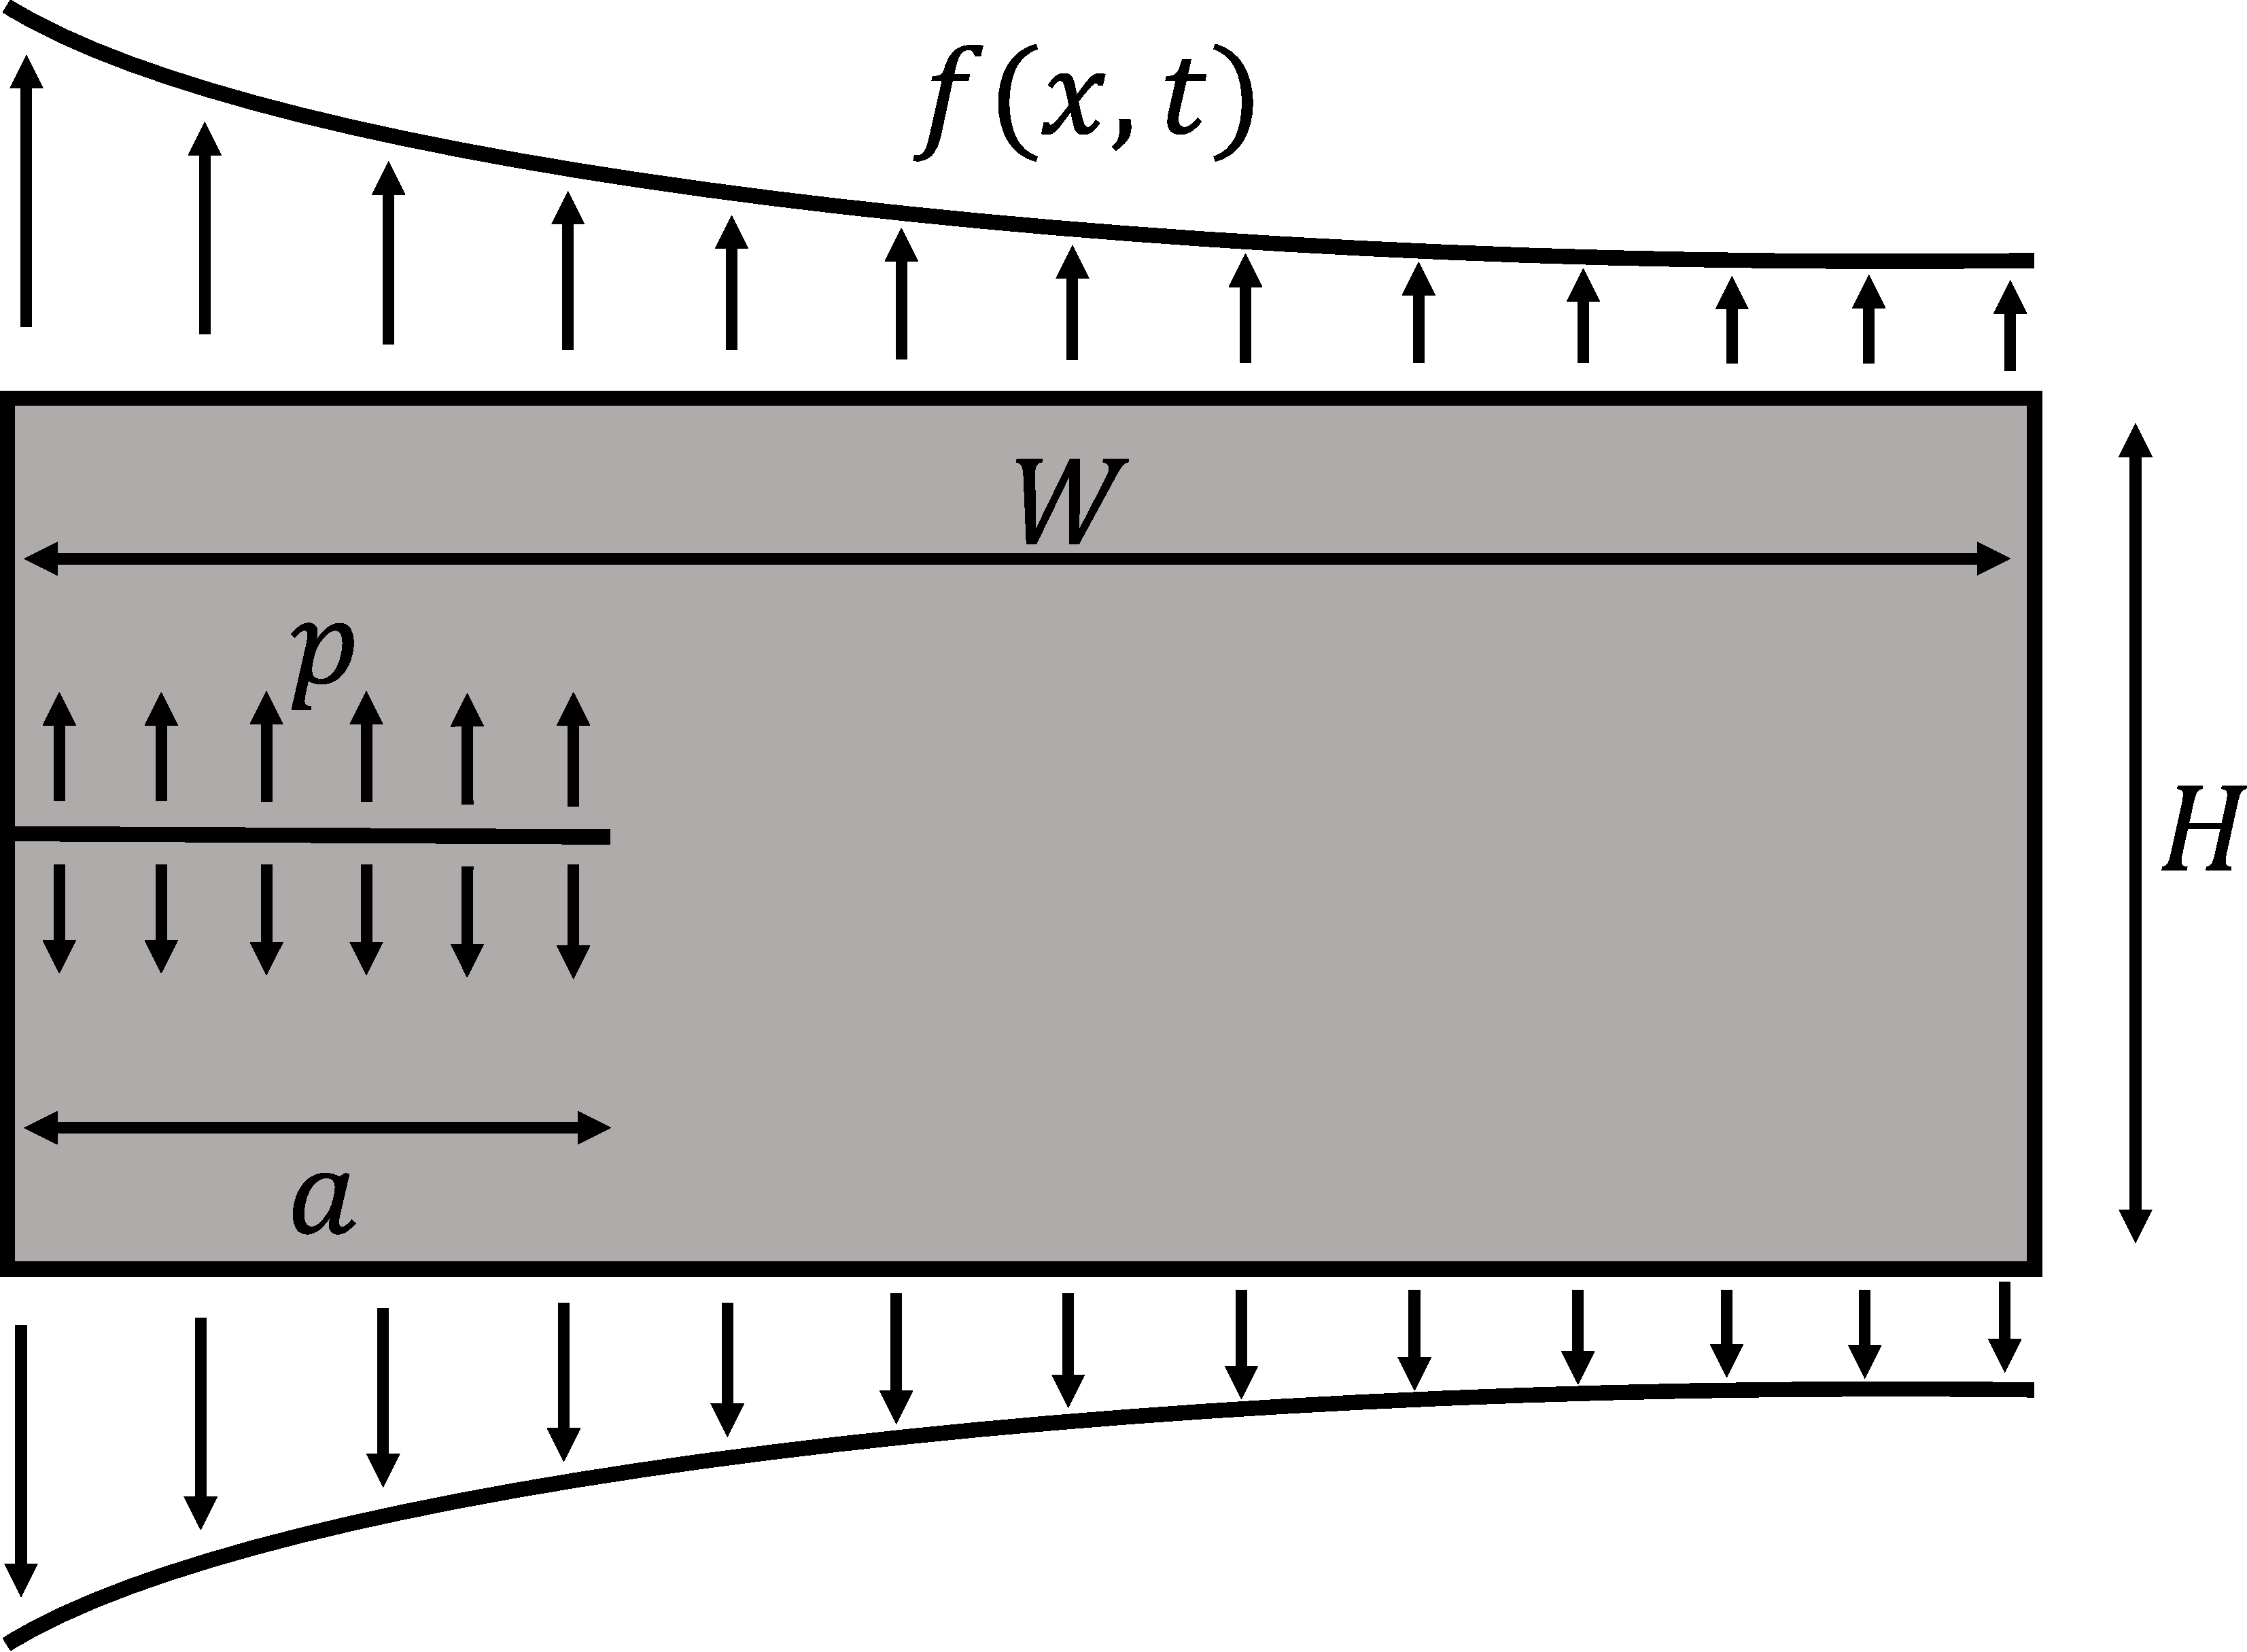
\includegraphics[width=0.8\linewidth]{images/2d_propagation/surfing_schematic.pdf}
  \caption{}
  \label{fig:surfing_schematic}
\end{subfigure}%
\begin{subfigure}{.49\textwidth}
  \centering
  \vspace{1.06cm}
  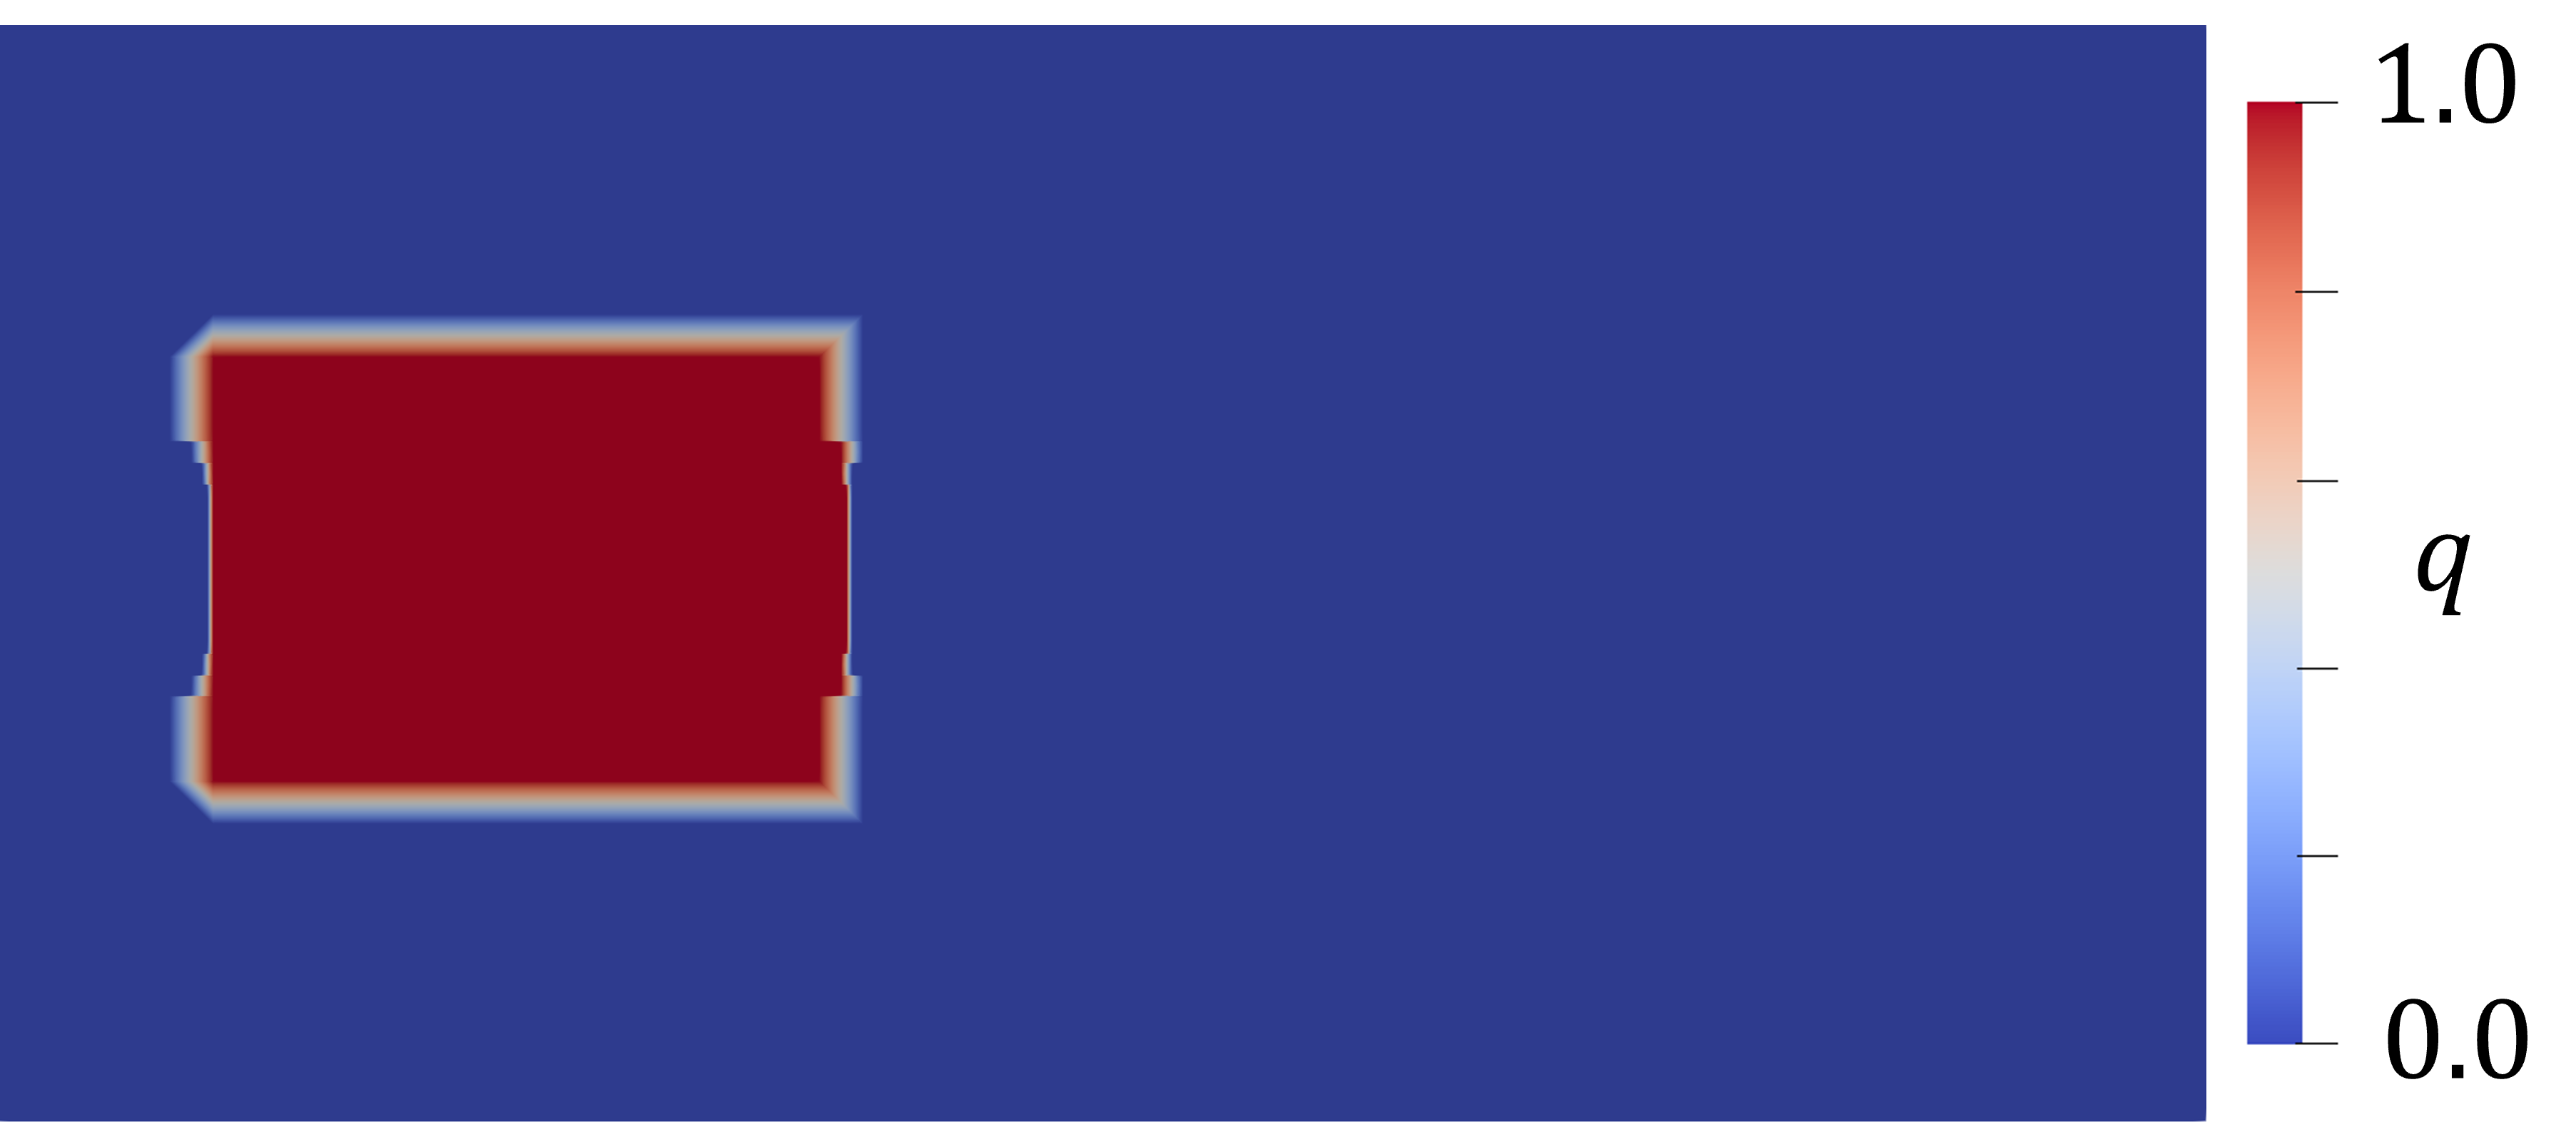
\includegraphics[width=0.8\linewidth]{images/2d_propagation/q_field_legend.png}
  \vspace{1.06cm}
  \caption{}
  \label{fig:integration_domain}
\end{subfigure}%
  \caption{(a) Geometry and boundary conditions for pressurized crack propagation problem; (b) J-Integral domain function $q$. } 
  \label{fig:surfing_problem_setup}
\end{figure}

\begin{table}[h]
\centering
\caption{Parameters used for pressurized crack propagation problem}
\begin{tabular}[t]{lcc}
\hline
&Value &Unit \\
\hline
Young's modulus ($\text{E}$)&3.0$\times10^4$&MPa\\
Poisson's ratio ($\nu$)&0.2&--\\
Critical fracture energy  ($G_c$)&0.12&$\text{mJ mm}^{-2}$\\
Initial crack length ($a$)&1.6&m\\
Specimen width ($W$)&8.0&m\\
Specimen height ($H$)&4.0&m\\
Target crack speed ($V$)&0.4&m/s\\
\hline
\end{tabular}\label{material_properties_propagation}
\end{table}

% The setup for this fracture propagation problem is the following. A rectangular strip with width $W$, height $H$ and a pre-crack of size $a$ is loaded by the ``surfing" boundary conditions in its top and bottom surfaces (Figure \ref{fig:surfing_schematic}). A pressure $p$, given by

% \begin{equation}
%     p = \dfrac{1}{2}\sqrt{\dfrac{G_cE'}{\pi a}},
% \end{equation}

% is applied on the crack faces.

% \begin{figure}[h]
% % \centering
% \begin{subfigure}{.49\textwidth}
%   \centering
%   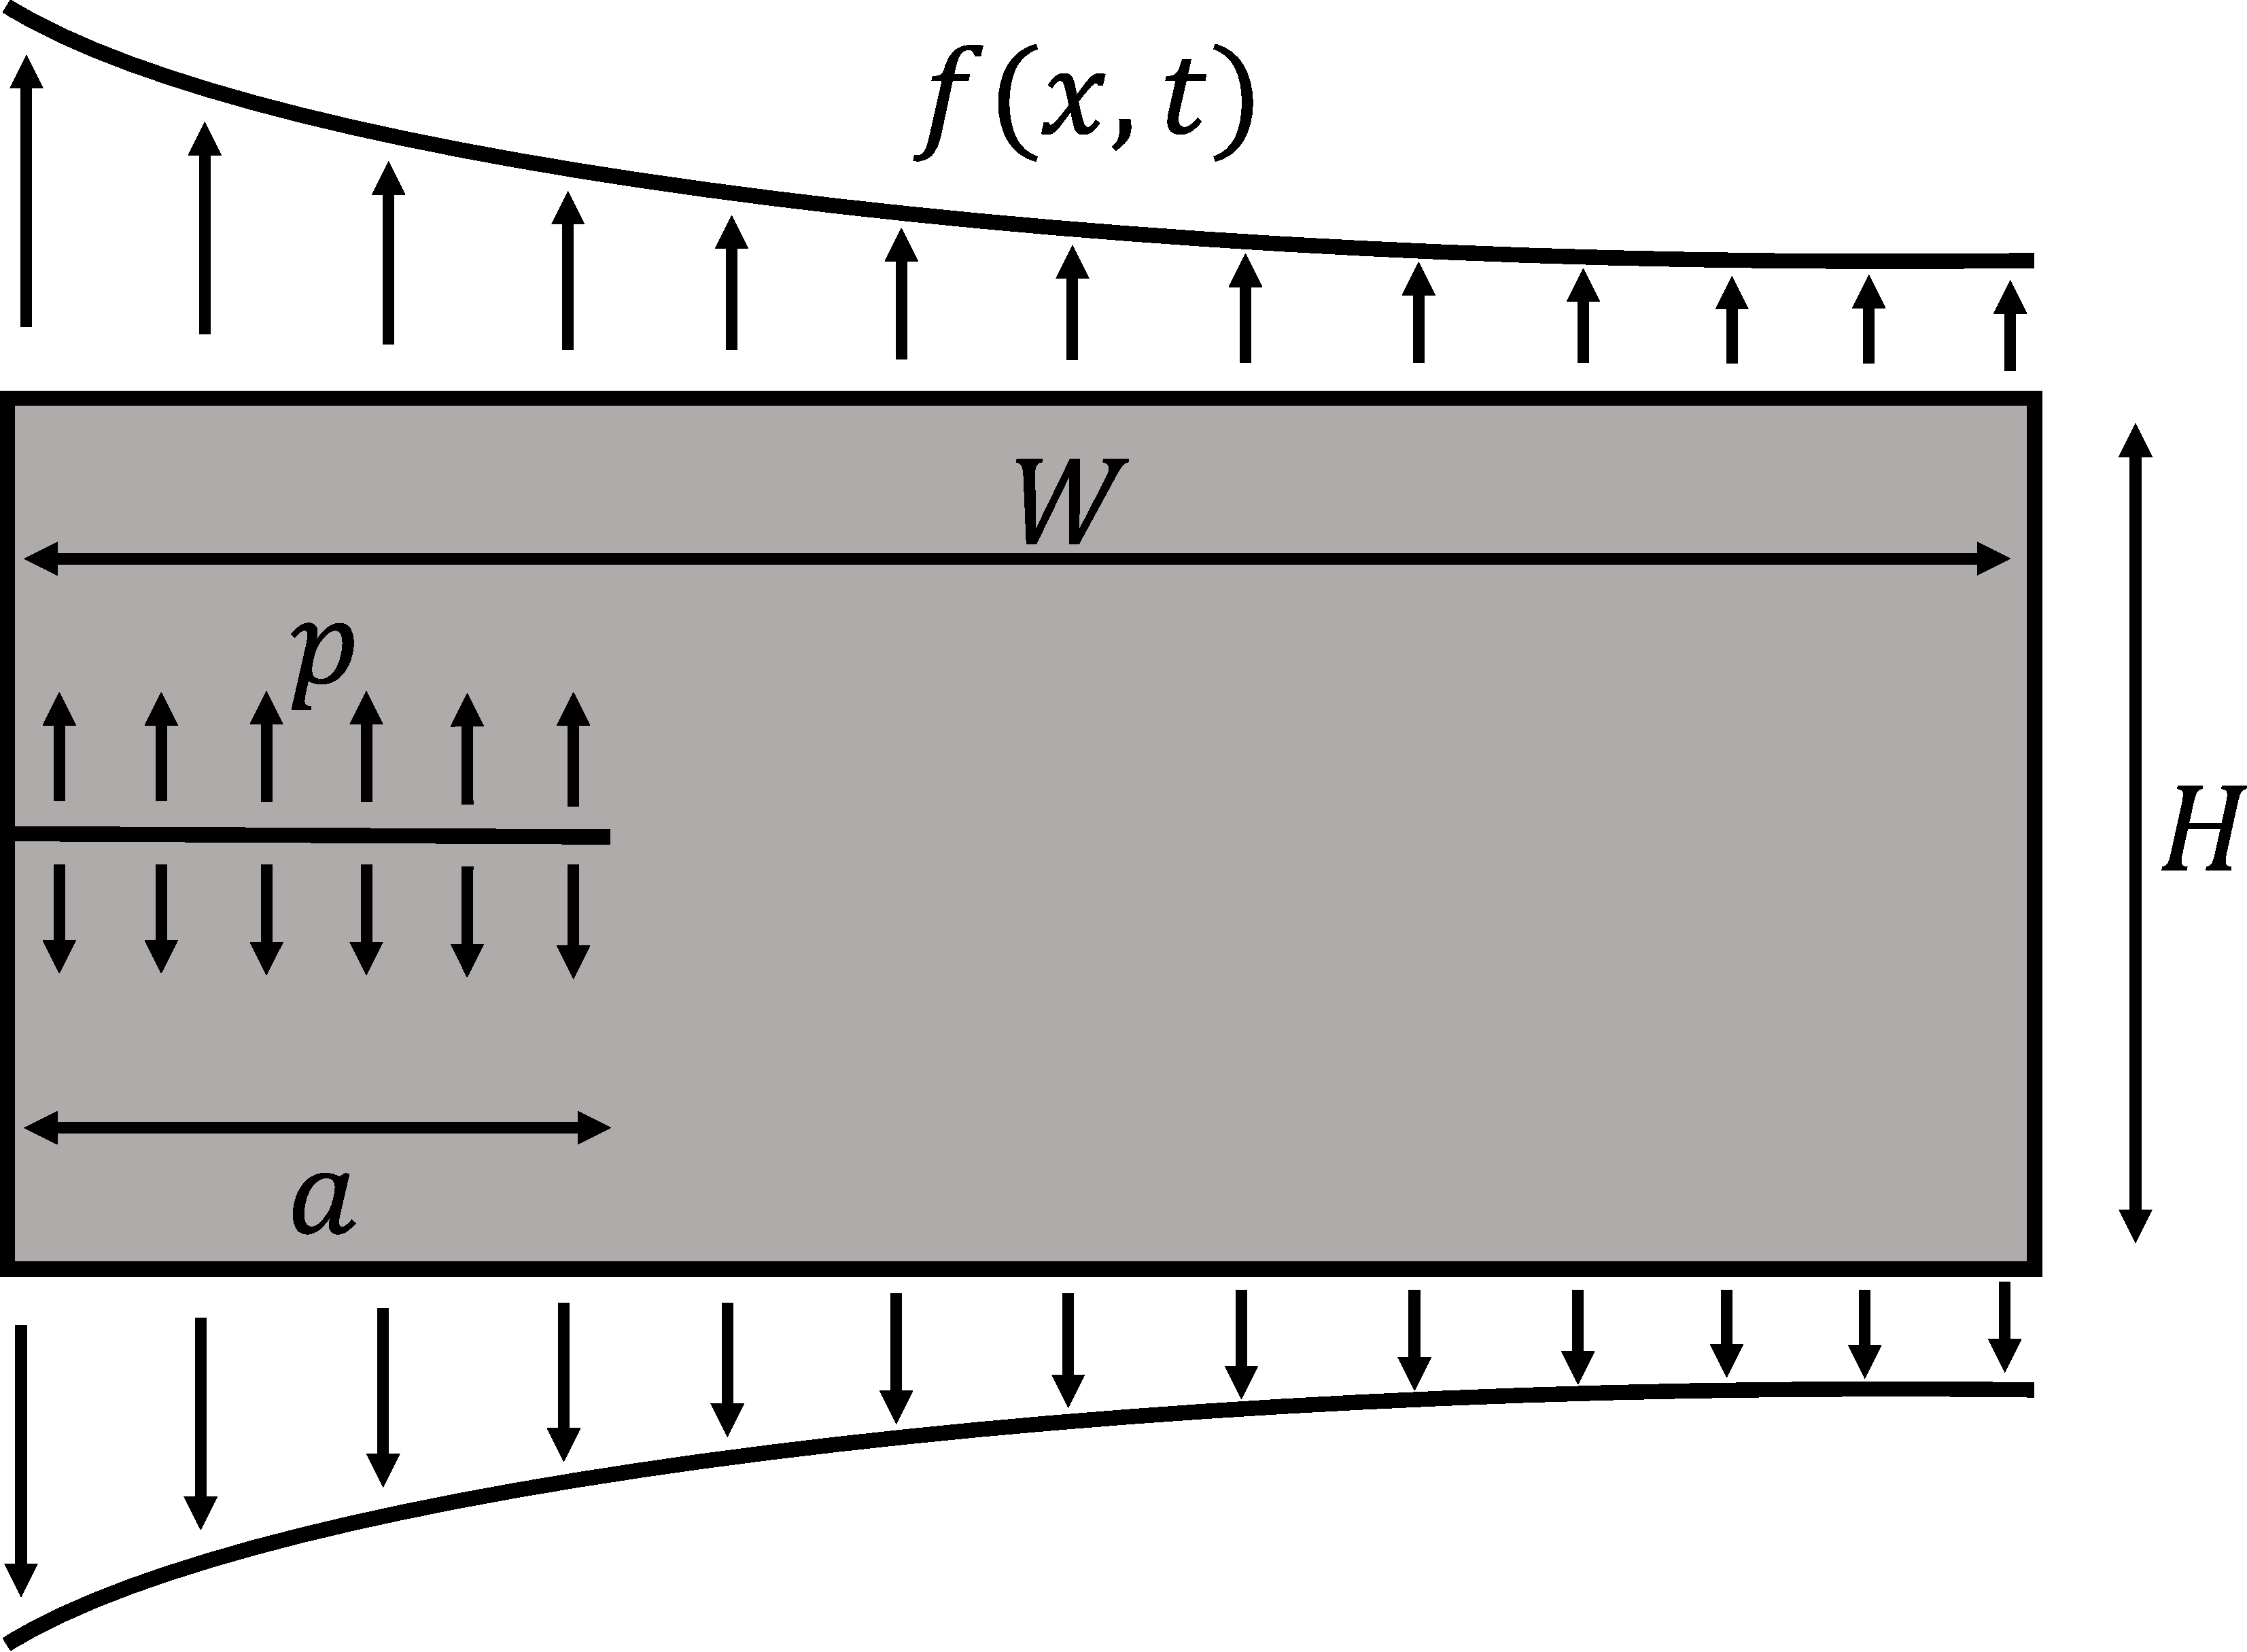
\includegraphics[width=0.8\linewidth]{images/2d_propagation/surfing_schematic.pdf}
%   \caption{}
%   \label{fig:surfing_schematic}
% \end{subfigure}%
% \begin{subfigure}{.49\textwidth}
%   \centering
%   \vspace{1.06cm}
%   \includegraphics[width=0.8\linewidth]{images/2d_propagation/q_field_wigly_legend.png}
%   \vspace{1.06cm}
%   \caption{}
%   \label{fig:integration_domain}
% \end{subfigure}%
%   \caption{(a) Problem schematic; (b) J-Integral domain function $q$ FIX LEGEND WITH LETTER D - do we really need this 2nd figure now?} 
%   \label{fig:surfing_problem_setup}
% \end{figure}

In order to verify that Griffith's law is approached as $\ell \rightarrow 0$, simulations are performed for this problem using a sequence of decreasing regularization lengths, ranging from $\ell = a/20$ to $\ell = a/160$. The mesh is locally refined along the $x$-axis, where the element size is set to $h = \ell/4$. The symmetry of the problem is exploited and only the response in the top half of the domain is simulated. 
% {\color{blue}In the early times ($t < 1$), the boundary condition \eqref{surfing_bc_1}-\eqref{surfing_bc_2} is ramped up with a factor of $t$, as that seem to facilitate convergence of the numerical solver.}{\color{red} This is how the surfing BC is implemented in raccoon, maybe we don't need to give this level of detail to the reader as it might confuse them?}
In terms of constitutive choices of the phase-field model, the AT-1 formulation is employed without any decomposition of the strain. 
%Although in general the phase-field system is non-convex, we found that, in this case, a simple monolithic approach based on Newton's method was able to converge, allowing for much faster simulations and tighter residual tolerances, which helped visualize the convergence of the results with respect to $\ell$. This scheme is therefore used in all cases of this subsection. 
As in the previous examples, this problem is analyzed using the formulations \eqref{lvc} and \eqref{uvc}, and the following choices of indicator function $I(d)$:
\begin{itemize}
    \item $I(d) = d$
    \item $I(d) = d^2$
    \item $I(d) = 2d-d^2$ 
\end{itemize}

To evaluate how well the models approach Griffith's law, the ratio between the energy release rate measured by the J-Integral and the effective critical fracture energy $G^{eff}_c = (1+2h/c_0\ell) G_c$ \footnote{in fact, phase-field cracks actually dissipated a slightly larger energy per unit length in numerical models. A correction factor of $\left(1+\dfrac{2h}{c_0\ell}\right)$ is then applied to $G_c$, following \cite{yoshioka2020crack}. The factor of 2 here comes from the symmetry boundary condition employed.} is plotted in Figures \ref{fig:prop_bourdin} and \ref{fig:prop_gary}.  In all figures, the time is scaled by a characteristic time $\tau$, defined as $\tau = a/V$. %Since the loading stage before the onset of propagation is not particularly important in this example, most of the that part ($t < 0.3\tau$) is omitted for better visualization of the results during the propagation phase.
The results using the traditional \eqref{lvc} formulation are presented in Figure \ref{fig:prop_bourdin}. They indicate convergence towards $J/G^{eff}_c$ = 1 as the regularization length is reduced, especially when the indicator function $I(d)=d$ is used. This is expected given the results obtained in \cite{bourdin2012variational}. Nevertheless, these results serve to verify the implementation of the J-Integral presented in Section \ref{sec:j_integral}. They also provide an estimate for how small the regularization length has to be in order to achieve a certain level of accuracy with these types of phase-field models.

\begin{figure}[h]
% \centering
\begin{subfigure}{.33\textwidth}
  \centering
  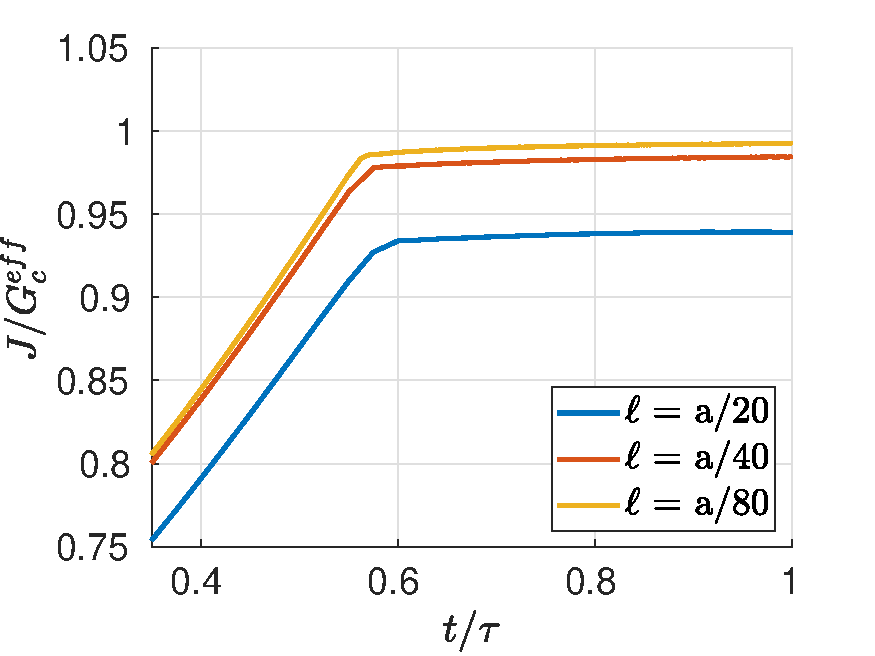
\includegraphics[width=\linewidth]{images/2d_propagation/zoom_bourdin_I_d.pdf}
  \caption{}
  \label{fig:prop_bourdin_d}
\end{subfigure}%
\begin{subfigure}{.33\textwidth}
  \centering
  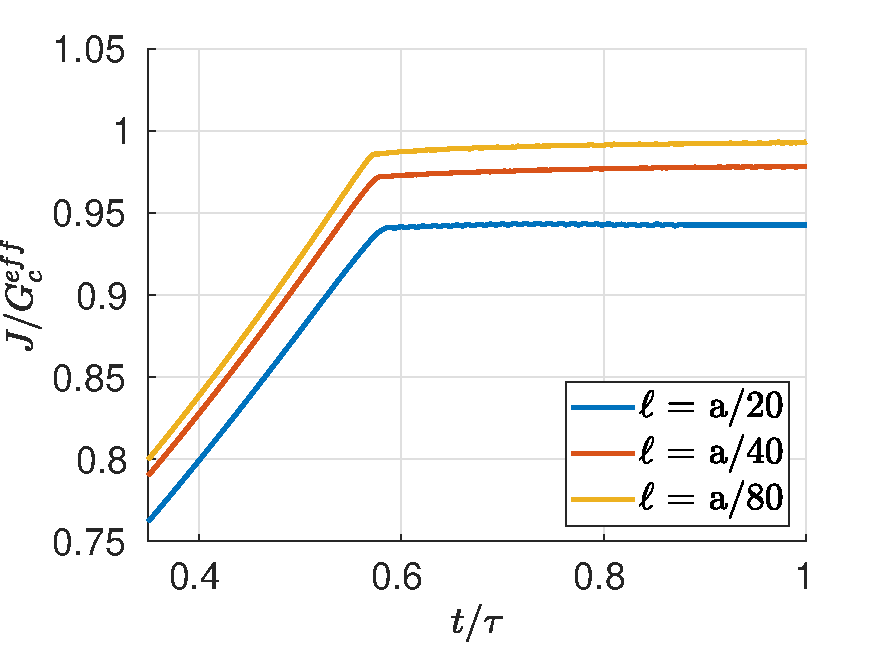
\includegraphics[width=\linewidth]{images/2d_propagation/zoom_bourdin_I_d2.pdf}
  \caption{}
  \label{fig:fig:prop_bourdin_d2}
\end{subfigure}%
\begin{subfigure}{.33\textwidth}
  \centering
  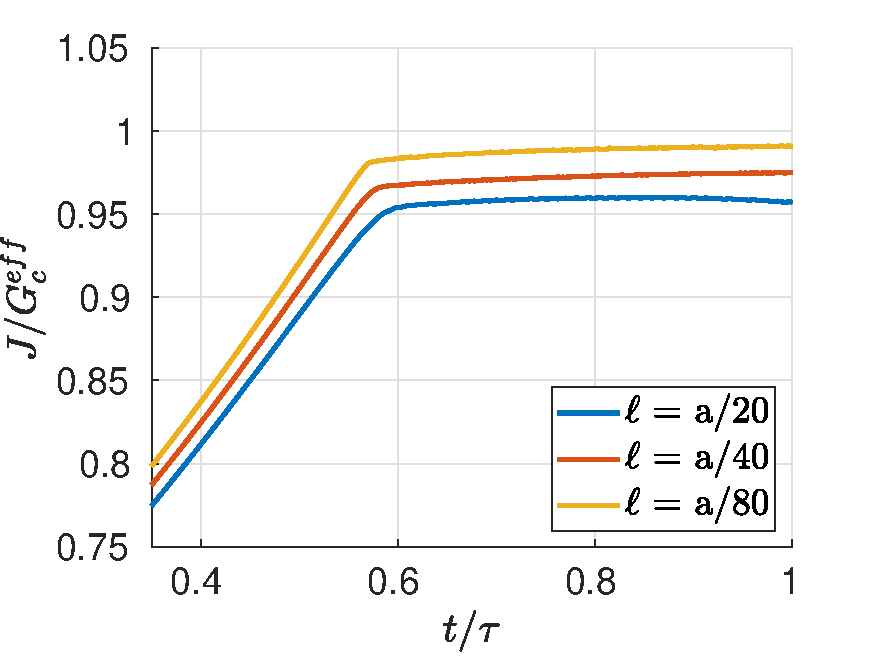
\includegraphics[width=\linewidth]{images/2d_propagation/zoom_bourdin_I_2d.pdf}
  \caption{}
  \label{fig:prop_bourdin_2d}
\end{subfigure}
  \caption{Reference results with the \ref{lvc} formulation. Curves with $\ell = a/160$ are not shown, as they are almost identical to the ones with $\ell = a/80$. (a) $I(d) = d$; (b) $I(d) = d^2$; (c) $I(d) = 2d-d^2$  } 
  \label{fig:prop_bourdin}
\end{figure}

\begin{figure}[h]
% \centering
\begin{subfigure}{.33\textwidth}
  \centering
  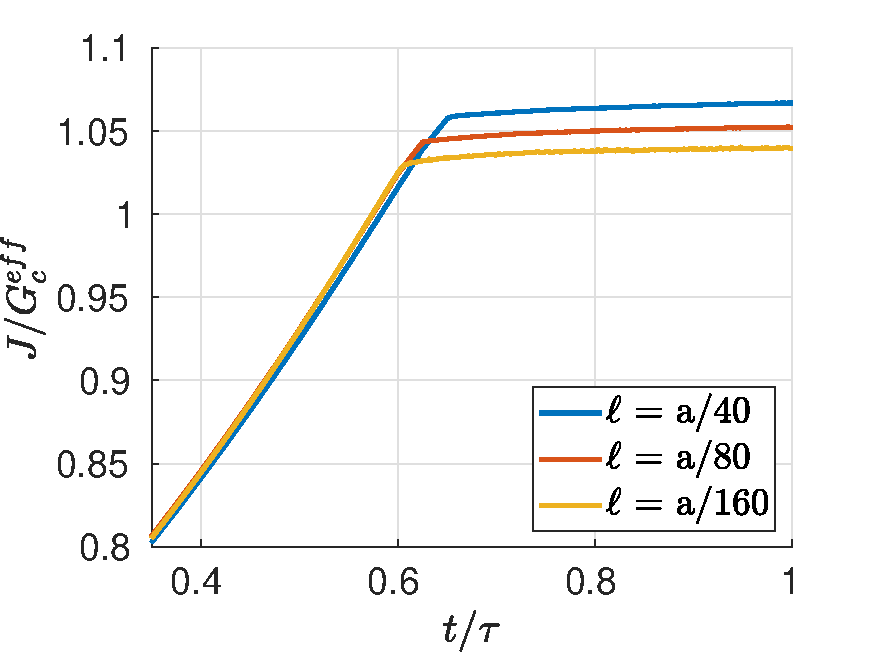
\includegraphics[width=\linewidth]{images/2d_propagation/zoom_gary_I_d.pdf}
  \caption{}
  \label{fig:prop_gary_d}
\end{subfigure}%
\begin{subfigure}{.33\textwidth}
  \centering
  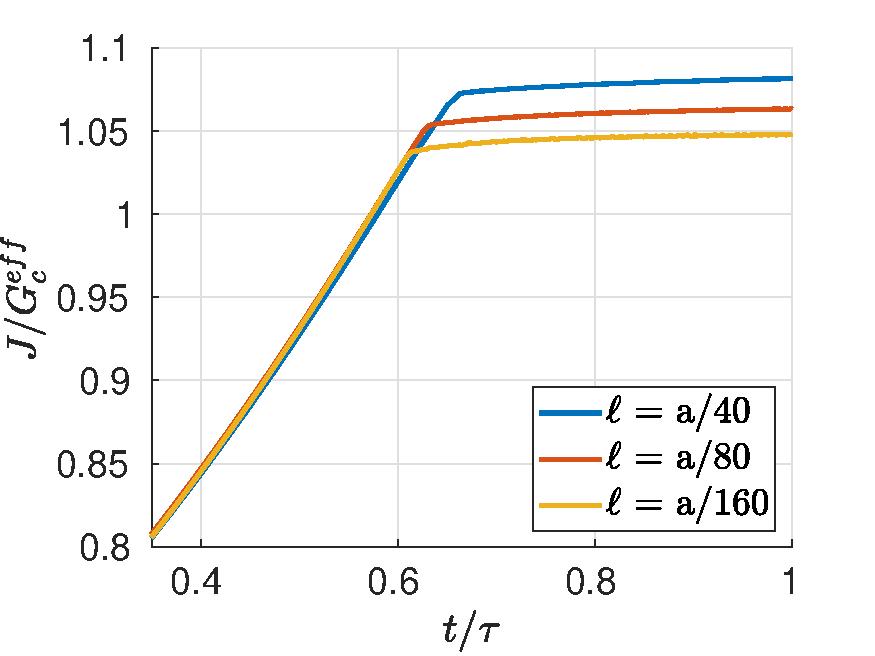
\includegraphics[width=\linewidth]{images/2d_propagation/zoom_gary_I_d2.pdf}
  \caption{}
  \label{fig:prop_gary_d2}
\end{subfigure}%
\begin{subfigure}{.33\textwidth}
  \centering
  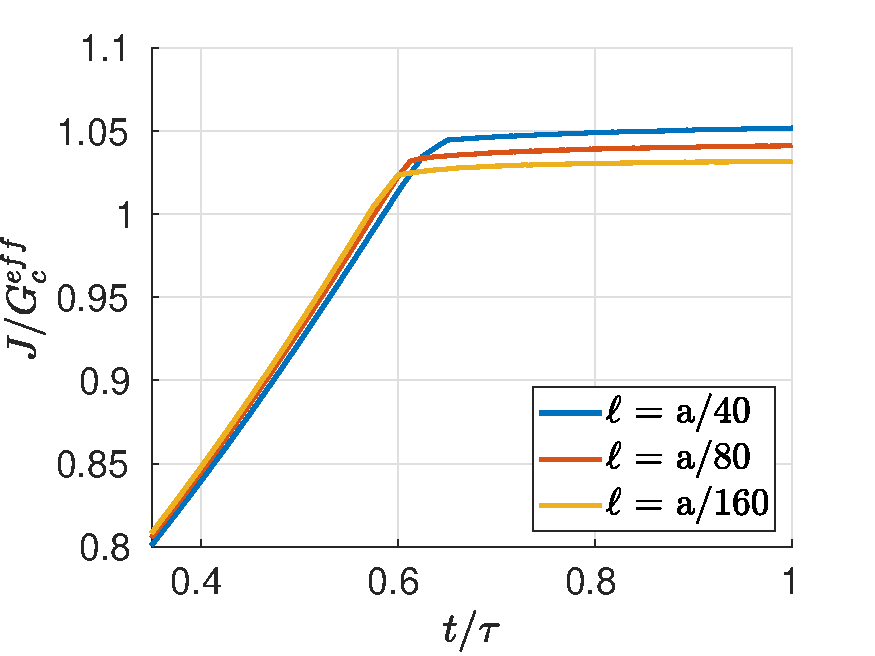
\includegraphics[width=\linewidth]{images/2d_propagation/zoom_gary_I_2d.pdf}
  \caption{}
  \label{fig:prop_gary_2d}
\end{subfigure}
  \caption{Results with the proposed formulation \eqref{uvc} (a) $I(d) = d$; (b) $I(d) = d^2$; (c) $I(d) = 2d-d^2$  } 
  \label{fig:prop_gary}
\end{figure}

% \begin{figure}[ht]

% \begin{subfigure}{.50\textwidth}
%   \centering
%   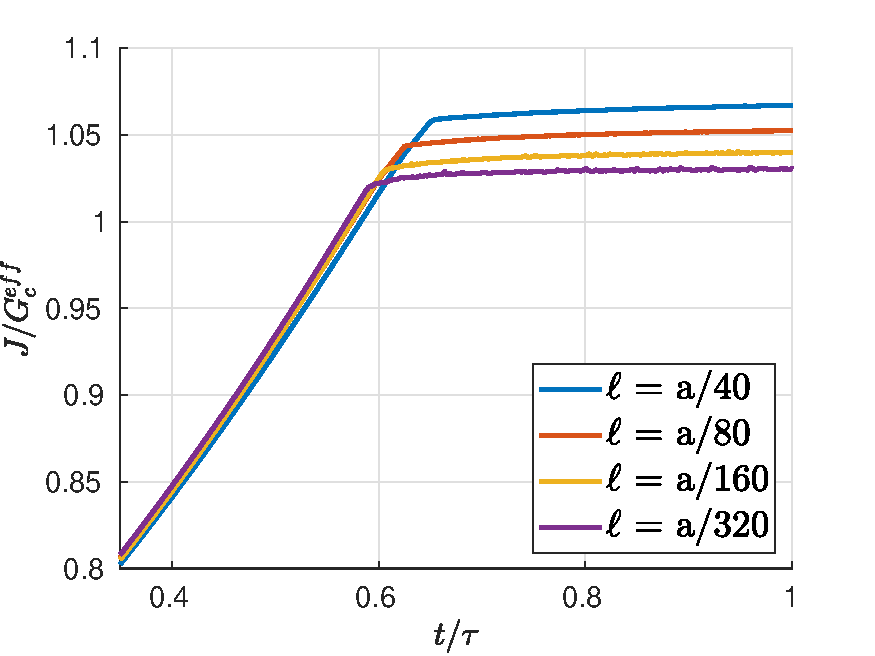
\includegraphics[width=\linewidth]{images/2d_propagation/zoom_fine_gary_I_d.pdf}
%   \caption{}
%   \label{fig:refined_gary_I_d}
% \end{subfigure}%
% \begin{subfigure}{.50\textwidth}

% \end{subfigure}
%   \caption{(a) Proposed formulation with $I(d) = d$. (b) Zooming in the portion where the crack begins to propagate.  } 
%   \label{fig:prop_gary_zoom}
% \end{figure}

\begin{figure}
  \centering
  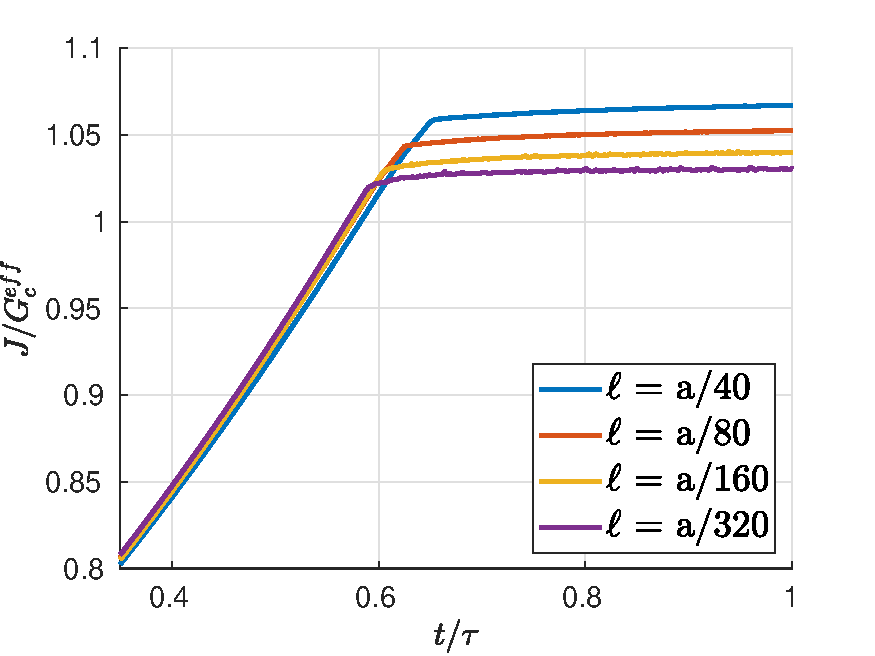
\includegraphics[width=0.7\linewidth]{images/2d_propagation/zoom_fine_gary_I_d.pdf}
  \captionof{figure}{Convergence of the proposed formulation with $I(d) = d$.}
  \label{fig:refined_gary_I_d}
\end{figure}

\begin{table}[h]
\centering
\begin{tabular}{ccc}
\hline
$\ell/a$ &Error &$\text{Error}_{k+1}/\text{Error}_{k}$ \\
\hline
1/40  & 0.067 & --\\
1/80  & 0.052 & 0.78\\
1/160 & 0.040 & 0.77\\
1/320 & 0.031 & 0.77\\
\hline
\end{tabular}
\caption{Absolute error in $J$ vs.\ $G_c^{eff}$ for the pressurized crack propagation problem, as a function of regularization length.}
\label{table:convergence_check}
\end{table}

For the case of proposed formulation \eqref{uvc}, the results shown in Figure \ref{fig:prop_gary} indicate a slower convergence towards a 
$J/G^{eff}_c = 1$ response. In contrast with the \eqref{lvc} formulation, the curves converge from above, and therefore, the fracture toughness is slightly overestimated when larger regularization lengths are used. Nevertheless, they all seem to approach a Griffith-like response in the limit $\ell \rightarrow 0$. In Figure \ref{fig:refined_gary_I_d}, an even finer result, using \eqref{uvc} with $I(d)=d$ and $\ell = a/320$ is added, to ensure that the convergence rates indicated in Figure \ref{fig:prop_gary} persist. In Table \ref{table:convergence_check}, the relative errors are provided, indicating a convergence rate of approximately $0.4$ with respect to $\ell$.

One potential explanation for the slower convergence rate is related to the different assumptions regarding the trial cracks, as discussed in Section \ref{sec:model}. Although the different assumptions converge to the same propagation rule in the limit of an infinitesimal crack increment, in the discretized case, the minimal crack increment is finite and related to the mesh spacing $h$ and regularization length $\ell$. In this case, a slightly different propagation behavior, resulting in slower convergence rates towards $J/G^{eff}_c = 1$ is not surprising. 
%In future work, a correction term, dependent on $h$ and $\ell$ will be investigated, in an attempt to improve this convergence rates and allow for better results in coarser meshes.


\section{Concluding Remarks}

This manuscript examines various models for phase-field fracture incorporating pressure loads on diffuse crack faces.  This includes the analysis of a new formulation that can be obtained by considering the presence of the pressure load in the virtual extension of a crack, or alternatively through a careful accounting in the minimization procedure. The new formulation is referred to as the 
 ``unloaded virtual crack formulation"\eqref{uvc}. In order to verify the accuracy of the various models for propagating cracks, a new form of the J-Integral for pressurized cracks in the phase-field context is derived.

The \eqref{uvc} formulation proposed herein allows for a unified treatment of crack nucleation and propagation in scenarios involving either brittle or cohesive fracture, and provides for better accuracy in some problems compared to existing formulations of the \eqref{lvc} type. As it allows for the use of the same governing equation for the damage parameter, its computational implementation within existing phase-field solvers is also simpler. In future work, its applicability to problems involving plastic deformation and strength-based fracture nucleation will be studied. In addition to that, modifications to accelerate the convergence of the model with respect to the phase-field parameter $\ell$ will also be considered.

\section{Acknowledgments}

%The authors would like to acknowledge the support and funding from Duke University and Argonne National Laboratory, which was essential to the development of this work.  
The partial support of A.\ Costa and  J.E.\ Dolbow by the National Science Foundation, through grant CMMMI-1933367 to Duke University, is gratefully acknowledged.  Author T.\ Hu gratefully acknowledges the support of Argonne National Laboratory.  Argonne National Laboratory is managed and operated by UChicago Argonne LLC.\ for the U.S.\ Department of Energy under Contract No.\ DE-AC02-06CH11357.

% \clearpage
\appendix
\chapter{Equivalence to SIF condition}\label{SIF_equivalence}

In this appendix, the energy release rate for a single, straight crack under an arbitrary pressure load $p(x)$ is computed, assuming that infinitesimal crack increments are traction-free, as shown in Figure \ref{fig:dry_crack}. Griffith's criterion states that propagation should happen whenever this energy release rate, which will be denoted by $G$, reaches $G_c$. This will give rise to a condition for propagation based on the pressure distribution $p(x)$, the crack size $a$ and Young's modulus $E'$\footnote{assuming plane strain, $E'=E/(1-\nu^2)$}. The purpose of the following derivation is to demonstrate that this condition is equivalent to the stress intensity factor criterion \cite{irwin1957analysis}.

Initially, consider the Sneddon-Lowengrub solution for the aperture of a pressure loaded crack in an infinite plate, under plane strain conditions,

\begin{equation}
    w(x) = \dfrac{4a}{\pi E'}\int^1_0p(sa)Z(x/a, s)\text{d}s
\end{equation}

\noindent where

\begin{equation}
    Z(r,s) = \log\left|\dfrac{\sqrt{1-r^2}+\sqrt{1-s^2}}{\sqrt{1-r^2}-\sqrt{1-s^2}}\right|
\end{equation}

\noindent is a convolution kernel. The work done by the pressure load is then,

\begin{equation}
    W_p = \int_{-a}^a p w \text{d}x = \int_{-a}^a p(y) \dfrac{4a}{\pi E'}\int^1_0p(sa)Z(x/a, s)\text{d}s\text{d}y.
\end{equation}

\noindent Clayperon's theorem \cite{fosdick2003} states that the potential energy is negative half of the work exerted in the boundary, which, in this case is only $W_p$. Hence

\begin{equation}
    U = -\dfrac{1}{2}W_p = -\dfrac{1}{2}\int_{-a}^a p w \text{d}x = -\dfrac{4a^2}{\pi E'}\int_{0}^1 p(ar)\int^1_0p(sa)Z(r, s)\text{d}s\text{d}r.
\end{equation}

% This expression is useful to compute $dU/\text{d}a$ for self-similar pressure fields.
% It can also be rewritten as,

% \begin{equation}
%     U = -\dfrac{4}{\pi E'}\int_{0}^a p(x)\int_0^a p(y)Z(x/a, y/a) \text{d}y\text{\text{d}x}
% \end{equation}

\noindent Let's write the energy release rate, assuming that the pressure field doesn't vary as the crack advances by a small amount $\text{d}a$. That is,

\begin{equation}
    p^{a+\text{d}a}(x) = 
    \begin{cases}
      p^{a}(x), & \text{if}\ x\le a \\
      0, & \text{if}\ a \le x \le a+\text{d}a
    \end{cases} 
\end{equation}

\begin{equation}
    dU = U(a+\text{d}a, p^{a+\text{d}a}) - U(a+\text{d}a, p^{a}), 
\end{equation}

\begin{multline}
       dU =  -\dfrac{4}{\pi E'}\int_{0}^{a+\text{d}a} p^{a+\text{d}a}(x)\int_0^{a+\text{d}a} p^{a+\text{d}a}(y)Z(\frac{x}{a+\text{d}a}, \frac{y}{a+\text{d}a}) \text{d}y\text{d}x \\ + \dfrac{4}{\pi E'}\int_{0}^a p^{a}(x)\int_0^a p^{a}(y)Z(x/a, y/a) \text{d}y\text{d}x.
\end{multline}

\noindent Using the definition of $p^{a+\text{d}a}$ given above,

\begin{equation}
       dU =  -\dfrac{4}{\pi E'}\int_{0}^{a} p^{a}(x)\int_0^{a} p^{a}(y)\left(Z(\frac{x}{a+\text{d}a}, \frac{y}{a+\text{d}a}) - Z(x/a, y/a)\right)\text{d}y\text{d}x.
\end{equation}

\noindent By symmetry, both tips of the crack propagate with the same energy release rate, so, one can write,

\begin{equation}
    2G = -\dfrac{dU}{\text{d}a} = \dfrac{4}{\pi E'}\int_{0}^{a} p^{a}(x)\int_0^{a} p^{a}(y)\dfrac{1}{\text{d}a}\left(Z(\frac{x}{a+\text{d}a}, \frac{y}{a+\text{d}a}) - Z(x/a, y/a)\right)\text{d}y\text{d}x.
\end{equation}

\noindent The term between parenthesis can be re-written as,

\begin{multline}\label{Z_difference}
    Z(\frac{x}{a+\text{d}a}, \frac{y}{a+\text{d}a}) - Z(x/a, y/a) = \\ \log\left|\dfrac{\sqrt{(a+\text{d}a)^2-x^2}+\sqrt{(a+\text{d}a)^2-y^2}}{\sqrt{(a+\text{d}a)^2-x^2}-\sqrt{(a+\text{d}a)^2-y^2}}\right| - 
    \log\left|\dfrac{\sqrt{a^2-x^2}+\sqrt{a^2-y^2}}{\sqrt{a^2-x^2}-\sqrt{a^2-y^2}}\right|\\
    = \log\left|\dfrac{\sqrt{(a+\text{d}a)^2-x^2}+\sqrt{(a+\text{d}a)^2-y^2}}{\sqrt{a^2-x^2}+\sqrt{a^2-y^2}}\right| \\ - 
    \log\left|\dfrac{\sqrt{(a+\text{d}a)^2-x^2}-\sqrt{(a+\text{d}a)^2-y^2}}{\sqrt{a^2-x^2}-\sqrt{a^2-y^2}}\right|.
\end{multline}

\noindent The second term contains a singularity, which can be removed if one re-writes it as,

\begin{multline}
    \log\left|\dfrac{\sqrt{(a+\text{d}a)^2-x^2}-\sqrt{(a+\text{d}a)^2-y^2}}{\sqrt{a^2-x^2}-\sqrt{a^2-y^2}}\right| = \\
    \log\biggl|\dfrac{\sqrt{(a+\text{d}a)^2-x^2}-\sqrt{(a+\text{d}a)^2-y^2}}{\sqrt{a^2-x^2}-\sqrt{a^2-y^2}} \\ \times \dfrac{\sqrt{(a+\text{d}a)^2-x^2}+\sqrt{(a+\text{d}a)^2-y^2}}{\sqrt{a^2-x^2}+\sqrt{a^2-y^2}} \\ \times \dfrac{\sqrt{a^2-x^2}+\sqrt{a^2-y^2}}{\sqrt{(a+\text{d}a)^2-x^2}+\sqrt{(a+\text{d}a)^2-y^2}} \biggr| \\
    = \log\biggl|\dfrac{(a+\text{d}a)^2-x^2-(a+\text{d}a)^2+y^2}{a^2-x^2-a^2+y^2}  \\ \times \dfrac{\sqrt{a^2-x^2}+\sqrt{a^2-y^2}}{\sqrt{(a+\text{d}a)^2-x^2}+\sqrt{(a+\text{d}a)^2-y^2}} \biggr|\\
    = - \log\left|\dfrac{\sqrt{(a+\text{d}a)^2-x^2}+\sqrt{(a+\text{d}a)^2-y^2}}{\sqrt{a^2-x^2}+\sqrt{a^2-y^2}} \right|.
\end{multline}

\noindent This expression can be plugged back into \eqref{Z_difference} to obtain,

\begin{multline}
    Z(\frac{x}{a+\text{d}a}, \frac{y}{a+\text{d}a}) - Z(x/a, y/a) = \\ \log\left|\dfrac{\sqrt{(a+\text{d}a)^2-x^2}+\sqrt{(a+\text{d}a)^2-y^2}}{\sqrt{(a+\text{d}a)^2-x^2}-\sqrt{(a+\text{d}a)^2-y^2}}\right| - 
    \log\left|\dfrac{\sqrt{a^2-x^2}+\sqrt{a^2-y^2}}{\sqrt{a^2-x^2}-\sqrt{a^2-y^2}}\right|\\
    = 2\log\left|\dfrac{\sqrt{(a+\text{d}a)^2-x^2}+\sqrt{(a+\text{d}a)^2-y^2}}{\sqrt{a^2-x^2}+\sqrt{a^2-y^2}}\right|.
\end{multline}

\noindent Hence,

\begin{multline}
    \dfrac{1}{\text{d}a}\left(  Z(\frac{x}{a+\text{d}a}, \frac{y}{a+\text{d}a}) - Z(x/a, y/a) \right) \\
    = \dfrac{2}{\text{d}a}\log\left|\dfrac{\sqrt{(a+\text{d}a)^2-x^2}+\sqrt{(a+\text{d}a)^2-y^2}}{\sqrt{a^2-x^2}+\sqrt{a^2-y^2}}\right|. 
\end{multline}

\noindent Now, the terms in the numerator can be expanded with a Taylor series,

\begin{equation}
    \sqrt{(a+\text{d}a)^2-x^2} = \sqrt{a^2-x^2} + \dfrac{a}{\sqrt{a^2-x^2}}\text{d}a + O(\text{d}a^2),
\end{equation}

\noindent leading to, 

\begin{multline}
    \dfrac{1}{\text{d}a}\left(  Z(\frac{x}{a+\text{d}a}, \frac{y}{a+\text{d}a}) - Z(x/a, y/a) \right) = \\
    \dfrac{2}{\text{d}a}\log\Biggl|\dfrac{\sqrt{a^2-x^2} + \dfrac{a}{\sqrt{a^2-x^2}}\text{d}a + O(\text{d}a^2)}{\sqrt{a^2-x^2}+\sqrt{a^2-y^2}} \\ + \dfrac{\sqrt{a^2-y^2} + \dfrac{a}{\sqrt{a^2-y^2}}\text{d}a + O(\text{d}a^2)}{\sqrt{a^2-x^2}+\sqrt{a^2-y^2}}\Biggr|,
\end{multline}

\noindent which, after using a Taylor expansion, simplifies to, 

\begin{equation}
    \dfrac{1}{\text{d}a}\left(  Z(\frac{x}{a+\text{d}a}, \frac{y}{a+\text{d}a}) - Z(x/a, y/a) \right) =  \dfrac{2a}{\sqrt{a^2-x^2}\sqrt{a^2-y^2}} + O(\text{d}a).
\end{equation}

% \begin{multline}
%     \dfrac{1}{\text{d}a}\left(  Z(\frac{x}{a+\text{d}a}, \frac{y}{a+\text{d}a}) - Z(x/a, y/a) \right) = \\
%     % = \dfrac{2}{\text{d}a}\log\left|\dfrac{\sqrt{a^2-x^2} + \dfrac{a}{\sqrt{a^2-x^2}}\text{d}a + O(\text{d}a^2)+\sqrt{a^2-y^2} + \dfrac{a}{\sqrt{a^2-y^2}}\text{d}a + O(\text{d}a^2)}{\sqrt{a^2-x^2}+\sqrt{a^2-y^2}}\right|
% \end{multline}

% \begin{multline}
%     \dfrac{2}{\text{d}a}\log\left|1 + \text{d}a\dfrac{\dfrac{a}{\sqrt{a^2-x^2}} + \dfrac{a}{\sqrt{a^2-y^2}}}{\sqrt{a^2-x^2}+\sqrt{a^2-y^2}} + O(\text{d}a^2)\right| = \dfrac{2}{\text{d}a}\log\left|1 + \text{d}a\dfrac{a }{\sqrt{a^2-x^2}\sqrt{a^2-y^2}} + O(\text{d}a^2)\right| \\
%     = \dfrac{2a}{\sqrt{a^2-x^2}\sqrt{a^2-y^2}}
% \end{multline}
     
\noindent Now, we can finally go back to the energy release rate,
    
\begin{multline}
    2G = -\dfrac{dU}{\text{d}a} = \dfrac{4}{\pi E'}\int_{0}^{a} p^{a}(x)\int_0^{a} p^{a}(y)\dfrac{2a}{\sqrt{a^2-x^2}\sqrt{a^2-y^2}} \text{d}y\text{d}x = \\
    \dfrac{8a}{\pi E'}\int_{0}^{1}\dfrac{p^{a}(ar)}{\sqrt{1-r^2}}\int_0^{1} \dfrac{p^{a}(as)}{\sqrt{1-s^2}} \text{d}s\text{d}r
    = \dfrac{8a}{\pi E'}\left( \int_{0}^{1}\dfrac{p^{a}(as)}{\sqrt{1-s^2}}\text{d}s\right)^2.
\end{multline}

\noindent From \cite{bazant2019fracture}, the stress intensity factor under these same conditions is,

\begin{equation}
    K_I = 2\sqrt{\dfrac{a}{\pi}}\left( \int_{0}^{1}\dfrac{p^{a}(as)}{\sqrt{1-s^2}}\text{d}s\right)
\end{equation}

\noindent From a simple inspection, one can see that $G = K_I^2/E'$, which guarantees the equivalence of the energy release rate criterion under the assumption in Figure \ref{fig:dry_crack} and the stress intensity factor condition. If instead, one assumes that the pressure load in the vicinity of a propagating crack behaves as in Figure \ref{fig:wet_crack}, this equivalence between the energetic criterion and the stress intensity factor may be violated.

% For a constant pressure,

% \begin{equation}
%     \mathcal{Z} = \dfrac{8a}{\pi E'}\left( \int_{0}^{1}\dfrac{p^{a}(as)}{\sqrt{1-s^2}}\text{d}s\right)^2 = \dfrac{8ap^2}{\pi E'}\left( \int_{0}^{1}\dfrac{1}{\sqrt{1-s^2}}\text{d}s\right)^2 =  \dfrac{8ap^2}{\pi E'}\dfrac{\pi^2}{4}\\
%     =  \dfrac{2\pi ap^2}{E'}
% \end{equation}
\chapter{A Multi-Resolution Approach for Hydraulic Fracture Simulation}
\label{section: Chapter3}

\section{Introduction}

A wide range of approaches for model-based simulations of hydraulic fracturing have been developed over the past several decades \cite{adachi2007computer, lecampion2018numerical}.  These range from production-level reservoir modeling tools such as  ResFrac\cite{mcclure2017three, mcclure2018resfrac}, to GEOS\cite{settgast2012simulation, settgast2014simulation, settgast2017fully}, PyFrac\cite{zia2020pyfrac}, and others.  Many of the models and associated codes assume fracture networks that remain planar, but in recent years strides have been made towards modeling cracks that evolve in arbitrary ways in response to fluid-driven loads. High-resolution models for complex fracture evolution generally fall into two categories: sharp interface models that explicitly model the fracture surface, and diffuse crack approaches that effectively smear the geometry over the underlying grid or mesh.  Techniques that represent the crack as a sharp interface can be advantageous when the fracture configuration is relatively simple, but representing complex geometric evolution can be challenging  \cite{gupta2014simulation, gupta2018coupled, shauer2022three}.  By contrast, diffuse crack models offer more flexibility for representing complex fracture evolution, but introduce other challenges such as the lack of a well-defined fracture surface and increased computational expense\cite{heider2021review}.  In this work, we introduce a multi-resolution scheme for hydraulic fracturing simulation that makes use of both sharp and diffuse crack representations within a single framework. The objective is to establish a methodology that makes use of the advantageous aspects of both sharp and diffuse crack models while circumventing some of the drawbacks.  

Over the past several decades, the phase-field model for fracture \cite{francfort1998revisiting, bourdin2000numerical, karma2001phase} has emerged as a promising approach for constructing robust simulations of complex crack evolution.  The method has shown considerable success for simulating fracture evolution in quasi-brittle materials, and there have been several recent efforts to extend the approach to hydraulic fracturing. In what follows, we review some prior works of particular relevance to the current manuscript.  For additional references in this topic, we refer the reader to the recent review by Heider \cite{heider2021review}.  

The first attempts towards a phase-field model for hydraulic fracture began with extensions of the traditional phase-field model to pressurized cracks, as in Bourdin et al. \cite{bourdin2012variational} and Wheeler et al. \cite{wheeler2014augmented}. Subsequently, fluid flow in the fractures, and also poromechanics were considered. Miehe et al. \cite{miehe2015minimization, miehe2016phase} developed a thermodynamically consistent framework, from minimization principles, to couple poromechanics, fluid-flow and phase-field fracture. The flow problem was modeled via the Darcy's equation, containing a permeability coefficient that used the phase-field variable and the crack opening to mimic the cubic relationship from the lubrication theory in the crack region. Mikelic et al. \cite{mikelic2015phase1, mikelic2015phase2} developed a model that separated the domain into fracture and reservoir, by using the phase-field variable as an indicator function. They also considered the flow inside the fracture as a Darcy flow, but their model treated the fracture as a three-dimensional entity, which led to a different permeability tensor compared to \cite{miehe2015minimization, miehe2016phase}.  Yet another approach concerns the work of Wilson and Landis \cite{wilson2016phase}, who proposed a model that included fluid velocities as primary variables. This allowed for a more detailed description of the flow within the fracture, which was modeled by a Brinkman-type equation \cite{brinkman1949calculation}. The phase-field parameter acted as an indicator of the flow regime, between Darcy flow (away from cracks) and Stokes flow (inside cracks).  Finally, the recent work of Chukwudozie et al.\ \cite{chukwudozie2019variational} presented a different model, wherein the lubrication theory equations were included in the weak form by means of a $\Gamma$-convergent regularization. 

The use of a phase-field to represent a fracture network in a diffuse manner certainly facilitates the representation of complex geometric evolution, including crack branching and merging. However, it also requires the use of meshes or grids that are capable of resolving the regularization length, making these approaches computationally expensive. One approach to improving the efficiency of the method is the use of adaptive mesh refinement, such as in \cite{heister2015primal, lee2017iterative, Wick-adaptive-2020,Gupta-adaptive-2022}. In the specific case of hydraulic fracturing, another challenge concerns the crack opening or aperture, a field that is tightly coupled with the fluid pressure within fractures. In a phase-field setting, due to the lack of an explicit crack surface, extracting the aperture or accounting for its effects requires additional considerations.  All of the aforementioned  works present some way to account for the aperture within a diffuse setting, but the robustness of these approaches remains unclear \cite{lecampion2018numerical}. For a review of the most frequently used methods to calculate the crack aperture from phase-field simulations, see the recent work of Yoshioka et al.\ \cite{yoshioka2020crack}.

Outside of the context of hydraulic fracturing, some researchers in the phase-field community have developed ``hybrid" approaches, wherein the phase-field formulation was combined with a sharp crack representation. The motivation for these approaches varies, from ``cutting" the mesh to remove artificial traction transmission and circumvent element distortion \cite{geelen2018optimization} to reducing the overall computational cost \cite{giovanardi2017hybrid, muixi2021combined}. In the work of Giovanardi et al.\ \cite{giovanardi2017hybrid}, phase-field subproblems in the vicinity of  crack tips were used to propagate a global, discrete crack. The eXtended Finite Element Method (XFEM)\cite{moes1999finite} was used to place fracture discontinuities in the displacement field within the background global mesh. More recently, Muixi et al.\ \cite{muixi2021combined} created an approach that uses the phase-field method only at the crack tips, and XFEM in the rest of the domain. In contrast to \cite{giovanardi2017hybrid}, there is no overlap of the representations in crack tip areas.

The success of these hybrid approaches for purely mechanical cases opens the door for their extension to hydraulic fracturing.  Such approaches are appealing because in principle they can circumvent the need for a complicated reconstruction of the crack opening from the phase-field.  This area is relatively unexplored, although there have been some recent efforts that are similar in spirit, such as the recent work of Sun et al.\ \cite{sun2020hybrid}.  They developed a Finite Element-Meshfree method to represent the crack surfaces in a discrete fashion. The computed displacement field was used to obtain a driving force which was employed within a phase-field evolution equation near the crack tips. This approach eliminated the need for the reconstruction of crack openings from the diffuse crack representation, but it also largely decoupled the phase field from the equations governing the force balance near the crack tips.  

The approach presented in this work, which we refer to as a multi-resolution method, extends the concept of a hybrid phase-field method to hydraulic fracturing. It discretizes the problem at a global level using a sharp interface approach based on the Embedded Finite Element Method of  Cusini et al.\ \cite{cusini2021simulation}.  It then approaches the simulation of fracture evolution by coupling the global fields with a phase-field fracture problem posed over a subdomain in the vicinity of the crack front.  This approach has several advantages.  The crack aperture and flow inside the fracture are handled at the global scale using techniques that work well and are efficient when the crack geometry is known.  Then the phase-field model is employed in the subdomain  to effectively update the crack geometry.  This framework lends itself to incorporation with a wide range of existing hydraulic fracturing solvers, as the phase-field sub-problem is agnostic about the type of numerical treatment used in the global domain. 
In the current work, we adopt relatively simple assumptions regarding material behavior, such as small deformations and linear poroelasticity, as they allow us to verify our scheme against analytical solutions. However, in principle the approach could be extended to model crack growth in a much broader class of poroelastic materials, such as hydrogels~\cite{Oyen:jop2021}. 

The paper is structured as follows. In Section \ref{formulation}, we present the governing equations and constitutive assumptions for both hydraulic fracturing and phase-field for fracture. In Section \ref{numerics}, we propose our multi-resolution framework and present numerical schemes to discretize both the hydrofracture and the phase-field subproblems. In Section \ref{results_section}, we apply our method to study hydraulic fracturing in some simple scenarios, in order to verify its accuracy. These include the well-known KGD\cite{geertsma1969rapid, zheltov19553} problems and a case of non-planar fracture propagation around a stiff inclusion. Finally, in Section 5, we provide a summary and some concluding remarks.




\section{Model formulation}\label{formulation}

In this section, we describe the models that are used to develop our multi-resolution scheme.  We start by presenting the governing equations to model hydraulic fracture in poroelastic rock that forms the basis for the solver at the global scale.  We then describe a phase-field model for fracture that forms the basis for the solver used in local subdomains near the crack tips.

\subsection{Governing equations for hydraulic fracture}

\begin{figure}[h]
    \centering
    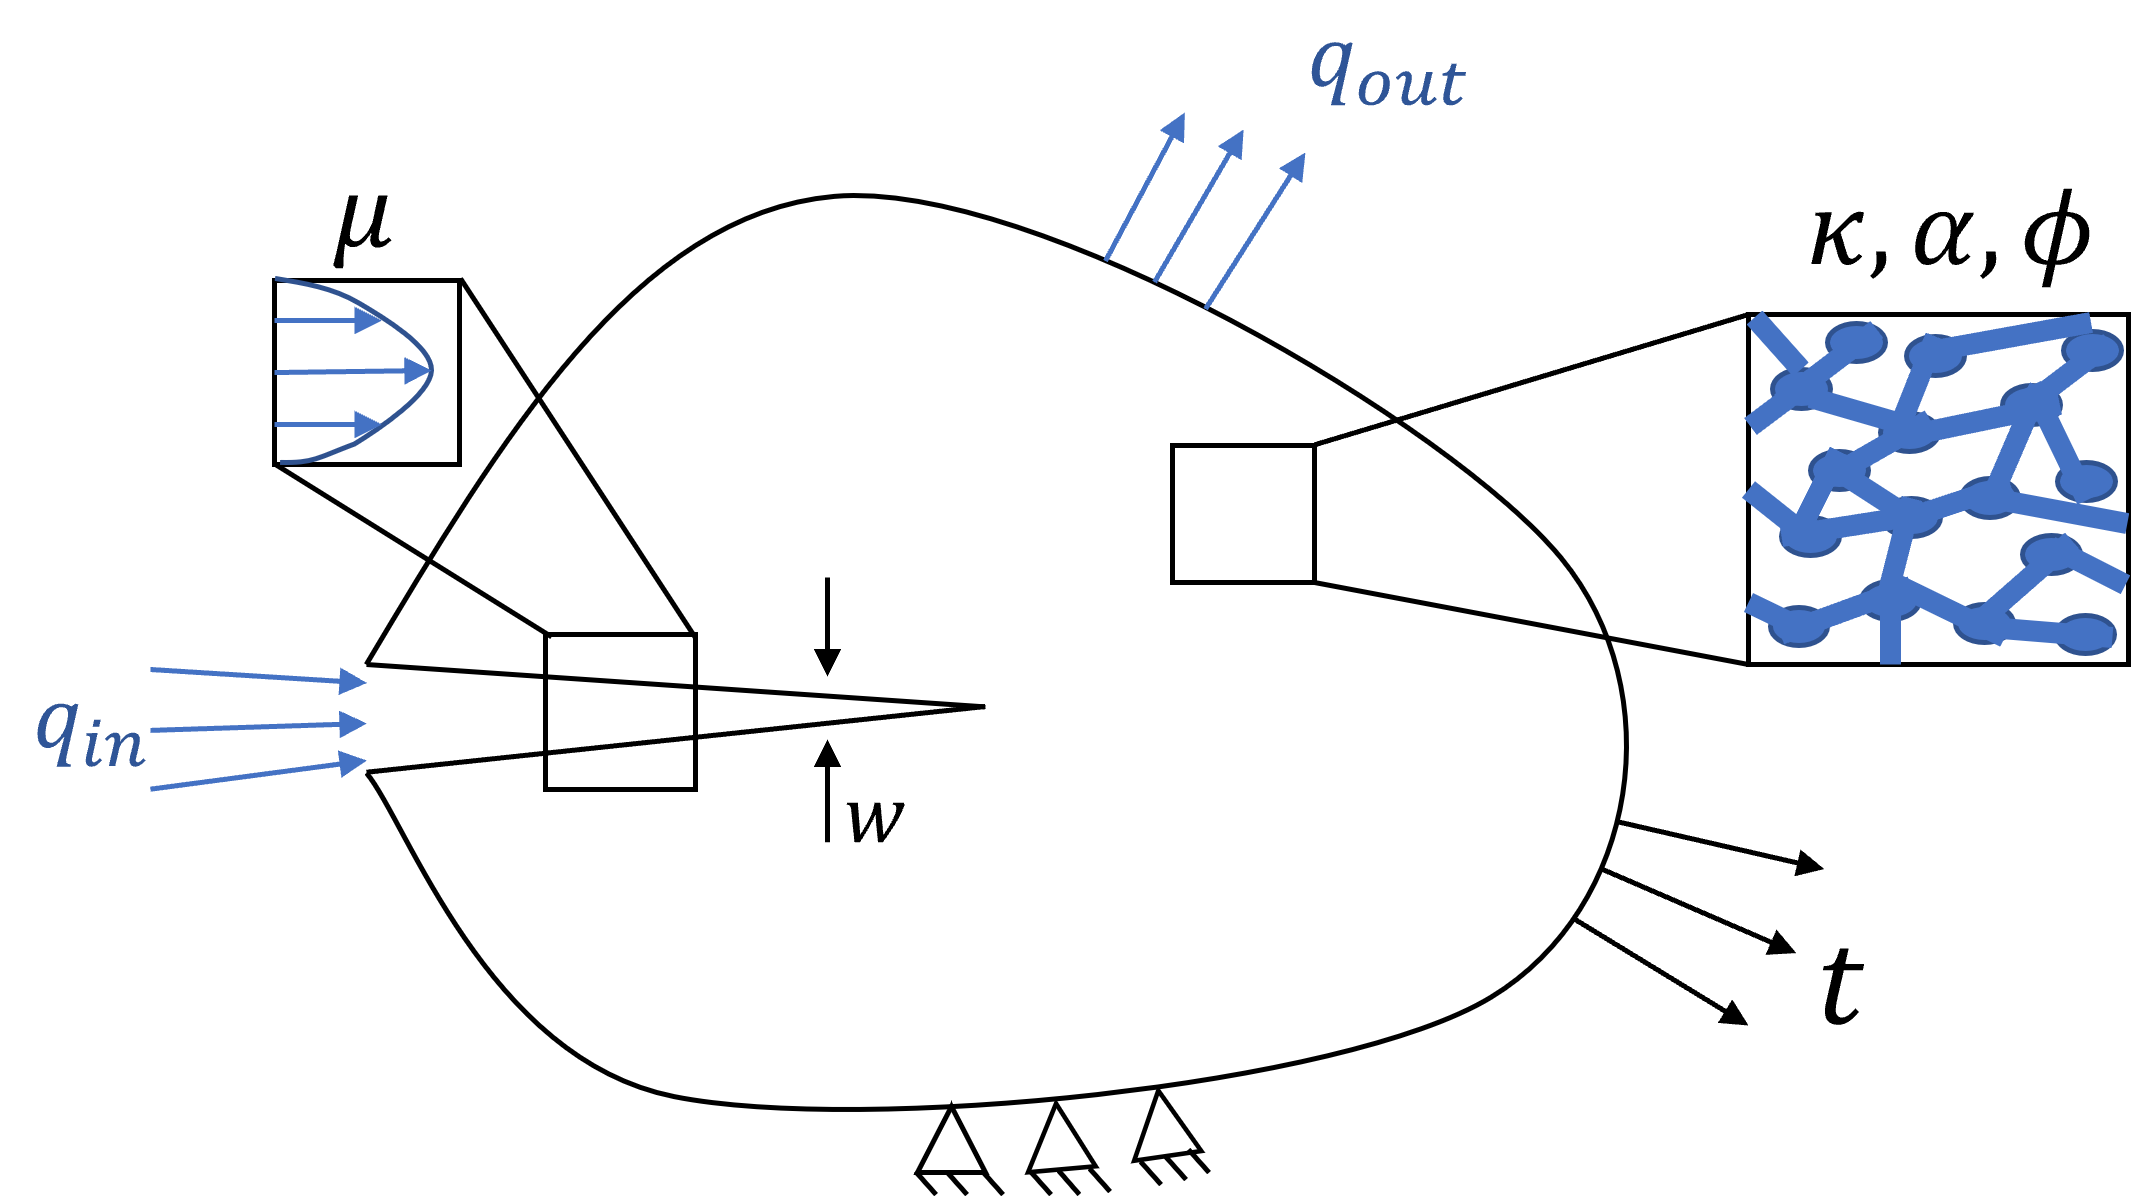
\includegraphics[width=15cm]{img/HF_potato_regular.png}
    \caption{Schematic of a poroelastic rock with a fracture, inspired by \cite{landis2016birs}.}
    \label{fig:potato_rock}
\end{figure}

We consider a model that couples flow and elastic deformation in a porous media with evolving fracture surfaces.  Consider the domain $\Omega$ consisting of a porous rock, that is fully saturated with a single-phase Newtonian fluid. The external boundary is composed of both traction $\partial \Omega_t$ and displacement $\partial \Omega_u$ surfaces, viz.\  $\partial \Omega = \partial \Omega_t \cup \partial \Omega_u$. 

The domain contains fractures $\Gamma$, as shown in Figure \ref{fig:potato_rock}.  For simplicity, we assume quasi-static conditions and small-strain kinematics.   Neglecting inertial effects, the balance of linear momentum reads
\begin{equation}\label{linear momentum balance}
    \nabla \cdot \boldsymbol\sigma + \textbf{b} = \boldsymbol 0\ \text{on } \Omega\setminus\Gamma,
\end{equation}
where $\boldsymbol\sigma$ denotes the total Cauchy stress and $\textbf{b}$ the body force. The mechanical boundary conditions are given by
\begin{equation}\label{traction bc}
    \boldsymbol \sigma \cdot \textbf{n} = \textbf{t} \text{ on } \partial \Omega_t,
\end{equation}
\begin{equation}\label{displacement bc}
    \textbf{u} = \overline{\textbf{u}} \text{ on } \partial \Omega_u,
\end{equation}

where $\textbf{n}$ denotes the normal direction at any point on $\partial\Omega$,  $\textbf{t}$ are the applied tractions, and $\overline{\textbf{u}}$ denotes the prescribed displacements.

Fluid flow within the cracks gives rise to pressure loads on the crack surfaces, translating into the boundary condition 
\begin{equation}\label{fracture boundary condition}
    \boldsymbol\sigma^+\cdot \textbf{n}_{\Gamma} = -\boldsymbol\sigma^-\cdot \textbf{n}_{\Gamma} = -p_f\textbf{n}_{\Gamma} \text{ on } \Gamma,
\end{equation}
where $p_f$ is the pressure inside the crack and $\textbf{n}_{\Gamma}$ is the normal vector to $\Gamma$ at any point.  In this work, we assume that fractures are open and neglect contact conditions on crack faces.  For additional considerations to account for closed fractures, see the model described in Cusini et al.\cite{cusini2021simulation}.

In terms of the fluid flow, the fluid velocity $\textbf{v}_m$ in the matrix is governed by the mass balance 
\begin{equation}\label{mass balance matrix}
    \dfrac{\partial(\rho \phi)}{\partial t} + \nabla \cdot (\rho \textbf{v}_m) = Q_m + Q_{mf}\ \text{on } \Omega\setminus\Gamma.
\end{equation}
where $\rho$ denotes the fluid density and $\phi$ is the porosity, and $Q_m$ is a prescribed source term in the matrix. The source term $Q_{mf}$ accounts for the exchange of fluid between the matrix and the fractures.
The boundary is partitioned into pressure $\partial \Omega_p$ and flux $\partial\Omega_q$ portions, such that $\partial \Omega = \partial \Omega_p \cup \partial \Omega_q$, and the following boundary conditions are applied,

\begin{equation}\label{flux bc}
    \rho \textbf{v}_m \cdot \textbf{n} = \textbf{q} \text{ on } \partial \Omega_q,
\end{equation}

\begin{equation}\label{pressure bc}
    p_m = \overline{p}_m \text{ on } \partial \Omega_p,
\end{equation}

where $p_m$ denotes the pore-pressure and  $\overline{p}_m$ is a prescribed pressure.

In a comparable manner, the fluid velocity $\textbf{v}_f$ within fractures is governed by the mass balance
\begin{equation}\label{mass balance fracture}
    \dfrac{\partial(\rho w)}{\partial t} + \nabla_{\Gamma} \cdot (\rho w \textbf{v}_f) = Q_f + Q_{fm}\ \text{on } \Gamma,
\end{equation}
where $w$ denotes the normal fracture aperture, $Q_f$ is a prescribed source term within the fracture, and $Q_{fm}$ accounts for the exchange of fluid between the fracture and the matrix\footnote{the flux interactions $Q_{fm}$ and $Q_{mf}$ are modeled as in classical well models, following \cite{hajibeygi2011hierarchical}. This ensures the balance of mass between the fractures and matrix $\int_V Q_{mf} dV = -\int_{\Gamma}Q_{fm}d\Gamma$.}. In the above, $\nabla_{\Gamma}$ indicates a gradient operator taken on the lower dimensional manifold  $\Gamma$. Boundary conditions similar to \eqref{flux bc} and \eqref{pressure bc} can also be applied.

Constitutive relationships are required to close the system and tie the stresses to the displacements $\textbf{u}$ and the fluid velocities to the pressures. In particular, we adopt the basic assumptions of Biot's theory of poroelasticity \cite{biot1941general}, Darcy's law for the flow in the matrix, and a lubrication theory approximation for the flow in fractures. This gives rise to the following set of constitutive relationships for the stress, porosity, and velocities:

\begin{equation}\label{biot law}
    \boldsymbol \sigma = \mathbb{C}:\boldsymbol\epsilon(\textbf{u}) - \alpha p_m \mathbb{I} \ \text{on } \Omega\setminus\Gamma,
\end{equation}

\begin{equation}\label{linear porosity}
    \dot{\phi} = \alpha \nabla \cdot \dot{\textbf{u}} + \dfrac{\dot{p_m}}{N} \ \text{on } \Omega\setminus\Gamma,
\end{equation}

\begin{equation}\label{darcy law}
    \textbf{v}_m = -\dfrac{\kappa}{\mu}\nabla p_m \ \text{on } \Omega\setminus\Gamma,
\end{equation}

\begin{equation}\label{cubic law}
    \textbf{v}_f = -\dfrac{w^2}{12\mu}\nabla_{\Gamma} p_f \ \text{on } \Gamma.
\end{equation}

In the above, $p_m$ is the pore-pressure, $\mathbb{C}$ is the fourth-order isotropic tensor of drained elastic moduli,  $\boldsymbol\epsilon(\textbf{u})$ is the mechanical strain, $\alpha$ is the Biot coefficient, and $\mathbb{I}$ is the second-order identity tensor. The temporal evolution of the porosity is governed by the rate of dilatation and time rate of change in the pore pressure, as modulated by the modulus $N$.  The fluid velocity in the matrix is related to the gradient of the pressure through the ratio of the intrinsic permeability $\kappa$ to the viscosity $\mu$.    

The fluid is assumed to be linearly compressible.  For both the fluid in the fractures and the matrix, this implies that the density is updated from its reference value $\rho_{ref}$ based on the change in pressure according to
\begin{equation}\label{poorly compressibility}
    \rho = \rho_{ref} \left(1 + \dfrac{p  - p_{ref}}{K_F}\right) \ \text{on } \Omega,
\end{equation}
where $p_{ref}$ denotes a reference value for the pressure, and $K_F$ is the fluid bulk modulus. 

Finally, the initial conditions for the displacements and pressures are given by

\begin{equation}\label{u_ic}
    \textbf{u}(\textbf{x},0) = \textbf{u}^0  \ \text{on } \Omega\setminus\Gamma,
\end{equation}

\begin{equation}\label{pm_ic}
    p_m(\textbf{x},0)= p^0_m  \ \text{on } \Omega\setminus\Gamma,
\end{equation}

\begin{equation}\label{pf_ic}
    p_f(\textbf{x},0) = p^0_f  \ \text{on } \Gamma.
\end{equation}

For a given crack geometry, the combination of equations \eqref{linear momentum balance}, \eqref{mass balance matrix} and \eqref{mass balance fracture}, with constitutive assumptions \eqref{biot law} - \eqref{poorly compressibility}, boundary conditions \eqref{traction bc}-\eqref{fracture boundary condition},\eqref{flux bc},\eqref{pressure bc} and initial conditions \eqref{u_ic}-\eqref{pf_ic} leads to a system of equations whose solution can be approximated by many different numerical methods.
What remains is a model to describe the evolution of the crack geometry.

In the context of standard sharp interface approaches for hydraulic fracture, the evolution of the crack geometry is typically governed by a set of criteria that dictate whether or not a crack front extends and, if so, in what orientation.  For crack extension, a standard approach is to adopt Griffith's criteria \cite{griffith1921vi}, which states that crack propagation should occur when the energy release rate $G$ reaches the critical value $G_c$ for the material, i.e.\ $G \le G_c$.   In terms of changes to orientation, several different criteria are typically employed, such as the maximum hoop stress criteria \cite{10.1115/1.3656897, williams1972fracture, finnie1973note} or the maximum energy release rate condition \cite{ewing1976further, cotterell1965brittle, hussain1974strain}. Examples of works from the hydraulic fracture field employing such criteria include \cite{he2018modeling, jang2020analysis, grossman2019algorithm}. 

Although such methods have seen some success in simulating the propagation of hydraulically-driven cracks, even in three dimensions \cite{gupta2014simulation, gupta2018coupled,shauer2022three}, they struggle as crack evolution becomes sufficiently complex.  By contrast, regularized methods have seen far more success in treating complex geometric evolution. In the next subsection, we present the governing equations for a phase-field method for fracture, a regularized approach for representing fractures and their evolution.  Phase-field for fracture models generally start from a single energetic postulate that generalizes Griffith's criteria, and which is able to describe the entire fracture propagation process.

\subsection{The phase-field method for fracture}
\label{sec:pfm-fracture}

The phase-field method for fracture started as an approximation \cite{bourdin2000numerical} to the variational approach for fracture by Francfort and Marigo \cite{francfort1998revisiting} for the quasi-static propagation of fracture in brittle materials. This model essentially states that a crack should evolve in a way that minimizes a total energy functional, among all admissible states, which are those that contain the current crack set (so that no healing is possible). For the method adopted in this work, we follow the work of Chukwudozie et al.\ \cite{chukwudozie2019variational} and associate the following total energy to a crack configuration $\Gamma$ in a poroelastic brittle solid $\Omega$:
% \begin{multline}\label{variational approach to fracture}
%     \mathcal{E}(\textbf{u}, p_m, p_f, \Gamma) = \int\limits_{\Omega \setminus \Gamma}W(\boldsymbol{\epsilon}(\textbf{u}), p_m)d\Omega - \int\limits_{\partial\Omega_N} \textbf{t} \cdot \textbf{u} ds
%     - \int\limits_{\Omega\setminus \Gamma} \textbf{b} \cdot \textbf{u} d\Omega \\
%     + \int\limits_{\Gamma}p_f \llbracket \textbf{u} \cdot \textbf{n}_{\Gamma} \rrbracket ds + G_c \mathcal{H}^{n-1}(\Gamma),
% \end{multline}
where the tractions applied to the boundary are denoted by $\textbf{t}$, the normal to the crack is denoted by $\textbf{n}_{\Gamma}$ and $\mathcal{H}^{n-1}(\Gamma)$ is the $n-1$ dimensional Hausdorff measure of $\Gamma$. 

The strain energy density $W(\boldsymbol{\epsilon}(\textbf{u}), p_m)$ is postulated as,

\begin{equation}
    W(\boldsymbol{\epsilon}(\textbf{u}), p_m) = \dfrac{1}{2}\left( \boldsymbol\epsilon(\textbf{u}) - \dfrac{\alpha}{nK} p_m\mathbb{I}\right) : \mathbb{C} : \left( \boldsymbol\epsilon(\textbf{u}) - \dfrac{\alpha}{nK} p_m\mathbb{I}\right),
\end{equation}

with $K$ denoting the bulk modulus and $n$ the system's dimension (2 or 3). The phase-field regularization, based on the Ambrosio-Tortorelli \cite{ambrosio1990approximation} functional is then performed by the introduction of the damage parameter $d$ and the regularization length $\ell$,

\begin{multline}\label{Poroelastic PF funcional}
    \mathcal{E}_{\ell}(\textbf{u},d,p_m,p_f) = \int\limits_{\Omega }\widetilde{W}(\boldsymbol{\epsilon}(\textbf{u}), p_m, d)d\Omega - \int\limits_{\partial\Omega_N}\textbf{t} \cdot \textbf{u} ds \\
    - \int\limits_{\Omega} \textbf{b} \cdot \textbf{u} d\Omega
    + \int\limits_{\Omega}p_f \textbf{u} \cdot \nabla d d\Omega 
    + \dfrac{G_c}{c_0}\int\limits_{\Omega }\left(\dfrac{\zeta(d)}{\ell} + \ell\nabla d\cdot\nabla d  \right)d\Omega,
\end{multline}

where the function $\zeta(d)$ is the local dissipation function, which is usually taken as $\zeta(d) = d$ or $d^2$. The constant $c_0$ is given by $c_0 = 4\int_0^1 \sqrt{\zeta(z)}dz$ and the regularized strain energy is defined by,

\begin{equation}\label{damaged strain energy}
    \widetilde{W}(\boldsymbol{\epsilon}(\textbf{u}), p_m, d) = \dfrac{1}{2}\left( (1-d)\boldsymbol\epsilon(\textbf{u}) - \dfrac{\alpha}{nK} p_m\mathbb{I}\right) : \mathbb{C} : \left( (1-d)\boldsymbol\epsilon(\textbf{u}) - \dfrac{\alpha}{nK} p_m\mathbb{I}\right),
\end{equation}

which is consistent with an assumption of damage arising in the sub pore scale \cite{chukwudozie2019variational}. Finally, our regularized crack evolution problem is then stated as a minimization principle for the functional $\mathcal{E}_{\ell}(\textbf{u},d,p_m,p_f)$, with respect to the variables $\textbf{u}$ and $d$, with the added condition that the damage process is irreversible and that the damage variable $d$ is bounded between the values of zero (undamaged state) and unity (fully broken state):
\begin{equation}\label{variational formulation of phase-field}
    \textbf{u}, d = \underset{\textbf{u},d}{{\operatorname{argmin}}} \ \mathcal{E}_{\ell}(\textbf{u},d,p_m,p_f)\ \text{,\ \   subject to } \dot{d} \ge 0, \text{ and } 0 \le d \le 1. 
\end{equation}

The following set of evolution equations can then be derived from the Karush–Kuhn–Tucker (KKT) \cite{karush1939minima, kuhn1951nonlinear} conditions:

\begin{equation}\label{basic u problem}
    \nabla \cdot \left( (1-d)^2\ \mathbb{C}:\boldsymbol\epsilon(\textbf{u}) -(1-d)\alpha p_m \mathbb{I}\right) + \textbf{b} = p_f\nabla d, 
\end{equation}

\begin{equation}\label{damage equation ch3}
    S_d \coloneqq  \dfrac{2G_c\ell}{c_0}\Delta d - \dfrac{G_c}{c_0\ell}\zeta'(d)-g'(d)W(\boldsymbol{\epsilon}(\boldsymbol{\textbf{u}}),0) + \alpha p_m\nabla \cdot \textbf{u} + \nabla \cdot (p_f\textbf{u}) \le 0,
\end{equation}

\begin{equation}
    \dot{d} \ge 0,
\end{equation}

\begin{equation}
   0 \le d \le 1,
\end{equation}

\begin{equation}
    S_d\dot{d} = 0,
    \label{eq:ddot-strong}
\end{equation}

with boundary conditions, $\boldsymbol\sigma \cdot \textbf{n} = \textbf{t}$ on $\partial \Omega_N$ and $(2G_c\ell\nabla d +c_0p_f\textbf{u})\cdot \textbf{n} \ge 0$ on $\partial \Omega$. The damaged stress is defined as $\boldsymbol\sigma = (1-d)^2\ \mathbb{C}:\boldsymbol\epsilon(\textbf{u}) -(1-d)\alpha p_m \mathbb{I}$.

In some cases, it is useful to decompose the energy \eqref{damaged strain energy} into positive and negative parts, in order to provide asymmetry between tension and compression states. In most problems studied in this manuscript, we found this decomposition to be important, and, unless otherwise mentioned, the spectral decomposition introduced in Miehe et al.~\cite{miehe2010phase} is used. With this decomposition, the equations for the macro-scale force balance \eqref{basic u problem} and the micro-force balance \eqref{damage equation ch3} are modified as

\begin{equation}\label{basic u problem spectral}\tag{22a}
    \nabla \cdot \left( (1-d)^2\ \mathbb{C}:\boldsymbol\epsilon^+(\textbf{u}) + \mathbb{C}:\boldsymbol\epsilon^-(\textbf{u})-(1-d)\alpha p_m \mathbb{I}\right) + \textbf{b} = p_f\nabla d, 
\end{equation}

\begin{equation}\label{damage equation spectral}\tag{23a}
    S_d \coloneqq  \dfrac{2G_c\ell}{c_0}\Delta d - \dfrac{G_c}{c_0\ell}\zeta'(d)-g'(d)W(\boldsymbol{\epsilon^+}(\boldsymbol{\textbf{u}}),0) - \alpha p_m\nabla \cdot \textbf{u} + \nabla \cdot (p_f\textbf{u}) \le 0,
\end{equation}

and the damaged stress becomes $\boldsymbol\sigma = (1-d)^2\ \mathbb{C}:\boldsymbol\epsilon^+(\textbf{u}) + \mathbb{C}:\boldsymbol\epsilon^-(\textbf{u})-(1-d)\alpha p_m \mathbb{I}$. In the above, $\boldsymbol\epsilon^+$ and $\boldsymbol\epsilon^-$ denote the positive and negative parts of the strain tensor as described in \cite{miehe2010phase}. 

Finally, to close this section, we note that the extent to which the solution to \eqref{variational formulation of phase-field} approaches a particular sharp model in hydraulic fracture in the limit as the regularization length $\ell\rightarrow 0$ has yet to be established.  Nevertheless, the particular phase-field model adopted here contains all of the requisite components to allow for a proof of concept of the multi-resolution approach.  






\section{Multi-resolution method }\label{numerics}

\subsection{General overview}

\begin{figure}[!htbp]
    \centering
    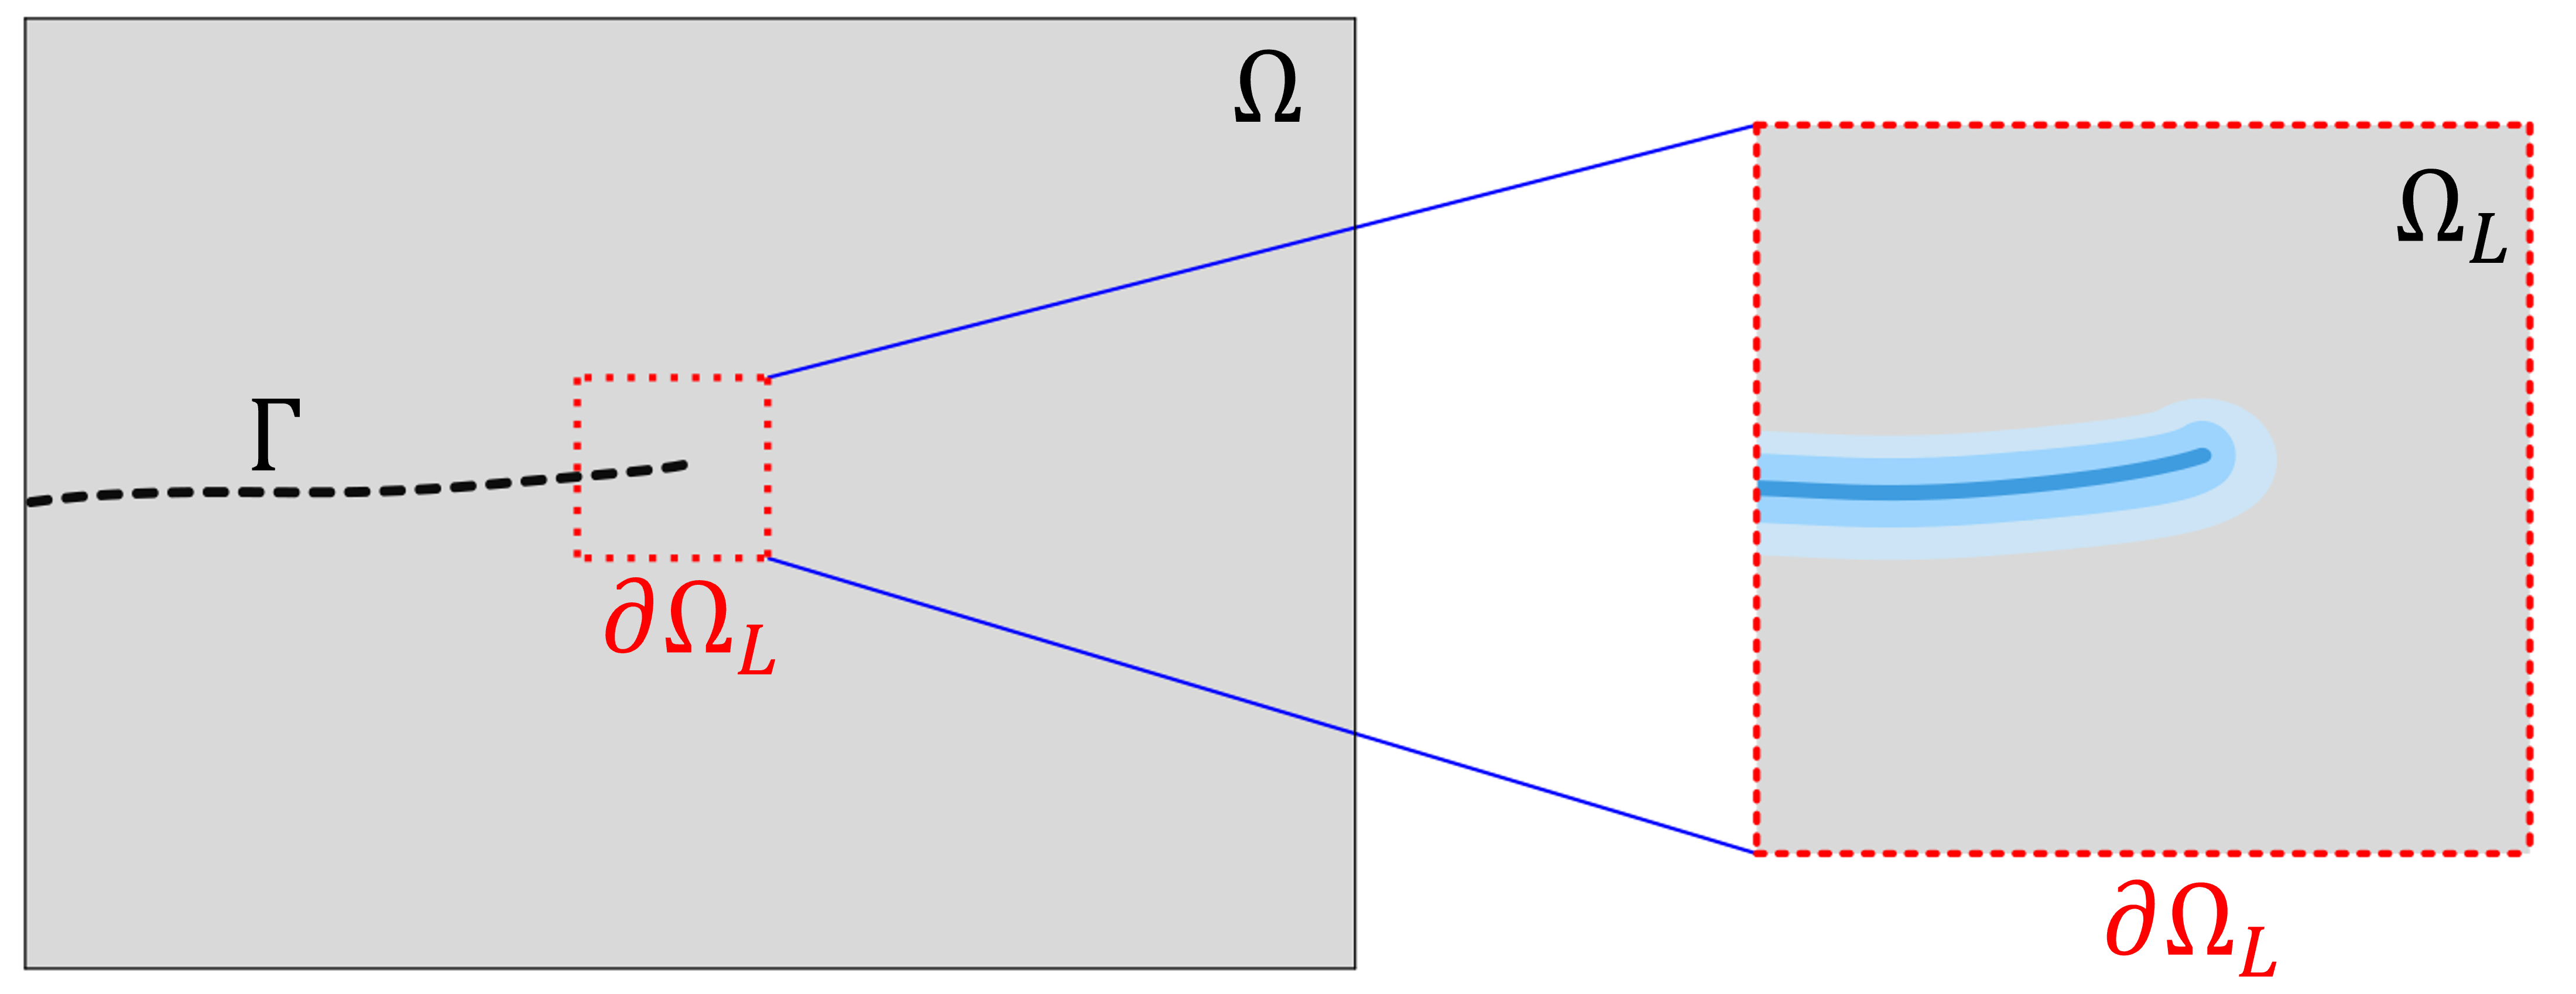
\includegraphics[width=\textwidth]{img/Section2/global_local_simple.png}
    \caption{Global domain $\Omega$ on the left and local domain $\Omega_L$ on the right. The surface corresponding to the local domain boundary $\partial\Omega_L$ is indicated within the global domain with the dashed red lines.  The local domain is magnified to highlight the phase-field representation of the global crack $\Gamma$.}
    \label{fig:section_2_figure}
\end{figure}

We propose a multi-resolution method to approximate the solution of the hydraulic fracture problem in porous media. It consists of coupling two problems between a global domain and a local subdomain, as shown in Figure~\ref{fig:section_2_figure}.   In the global domain problem, the governing equations \eqref{linear momentum balance}-\eqref{mass balance fracture} are discretized, and the crack is represented with a sharp geometry.  The crack geometry is assumed to be fixed during a solution step in the global domain, and relevant fields are calculated over the entire domain.  

By contrast, the local subdomain concerns only a portion of the entire domain, namely in the vicinity of crack tips.  It is encapsulated within the global domain as shown in Figure~\ref{fig:section_2_figure}. In the local subdomain, a discretization of the variational principle \eqref{variational formulation of phase-field} is used to simulate crack evolution.  During a solution step in the local subdomain, the pressure fields within the fracture and matrix are assumed to be fixed.  

The two problems are coupled in the following manner.  The displacement and pressure fields are extracted from a solution step in the global domain and passed to the local subproblem in different ways.  In particular, the global displacement fields are extracted along the surface $\partial\Omega_L$. These fields are then  applied as Dirichlet boundary conditions for the local subproblem.  The matrix pressure $p_m$ and pressure in the fracture $p_f$ are transfered as fields from the global domain to the local subdomain (see Section~\ref{sec:pressure_projection} for details), and assumed to be fixed for the local subproblem.   

The aforementioned operations provide everything that is needed for the local subproblem from the global domain.  Based on the imprint of the global crack geometry on the local subdomain, a regularized fracture surface is created (through an initial damage field) and then crack propagation is simulated in the local subdomain. Once an extension of the crack in a scale that can be represented in the global domain is identified, the sharp crack geometry in the global problem is updated accordingly.  

In principle, the aforementioned multi-resolution approach can be implemented using a number of different discretization methods in the global domain and the local subdomain.  In the sections that follow, we describe the particular choices used in this work as well as some important implementation details.  The method is described in a two-dimensional context, but many aspects can be readily extended to three-dimensional problems.  

\subsection{Global problem discretization}
\label{sec:global_disc}

The global problem in our multi-resolution approach encompasses the physics of fluid flow in both the fractures and the pore structure of our domain, as well as the deformation of the solid media. The set of governing equations consists of  \eqref{linear momentum balance}-\eqref{mass balance fracture}, combined with constitutive assumptions \eqref{biot law}-\eqref{poorly compressibility} and appropriate boundary conditions. 

In this work, we use the discretization method proposed by Cusini et al.\ \cite{cusini2021simulation} in the study of fluid flow in fractured porous media. 
The  domain $\Omega$ is partitioned with a  mesh $\mathcal{T}$. Then, the intersection of the fracture network $\Gamma$ with $\mathcal{T}$ defines the fracture triangulation $\mathcal{F}$. These meshes are then used to define discrete counterparts $\textbf{u}^h_G$, $p_m^h$ and $p_f^h$ of the unknown fields $\textbf{u}$, $p_m$ and $p_f$, as well as discrete approximations of equations  \eqref{linear momentum balance}, \eqref{mass balance matrix} and \eqref{mass balance fracture}.

A finite element approximation is constructed for the displacement field and employed in a standard Galerkin approximation to the global force balance \eqref{linear momentum balance}. The continuous part of the displacement field is approximated with a standard space $\mathcal{U}$  of 4-node bilinear shape functions $\{ {\boldsymbol{\eta}}_a \} $.  In the subset of elements that are ``cut" by the global crack geometry, a space $\mathcal{W}$ of discontinuous enrichment functions $\{\boldsymbol{\phi}_b\}$ is constructed using the formulation described in \cite{linder2007finite}.   

The full displacement field in the global problem is constructed using both continuous and discontinuous parts as
\begin{equation}
    \label{eq:displacement_approx}
    \textbf{u}^h_G = \underbrace{\sum_{a=1}^{n_u}u_a \boldsymbol{\eta}_a}_{\text{continuous part}} + \underbrace{\sum_{b=1}^{n_w}w_b\boldsymbol\phi_b}_{\text{discontinuous part}}, 
\end{equation}
where $\{u_a\}, \{ w_b\}$ are scalar degrees of freedom. 

The flow equations  \eqref{mass balance matrix} and \eqref{mass balance fracture} are discretized with a finite-volume method.   Piecewise-constant pressure fields are constructed for $p_m^h$ and $p_f^h$ over the matrix mesh $\mathcal{T}$ and the fracture mesh $\mathcal{F}$, respectively. Fluxes are computed using a two point flux approximation. The interaction between the flow in the fracture and matrix is effected via the embedded discrete fracture model (EDFM) \cite{lee2001hierarchical, hajibeygi2011hierarchical}. 

In terms of the temporal discretization, the parabolic nature of equations \eqref{mass balance matrix} and \eqref{mass balance fracture} gives rise to a stable time step for explicit schemes that scales with the cube of the mesh spacing \cite{adachi2007computer, lecampion2018numerical}. This upper bound is prohibitively small in most cases. Therefore, an implicit backward Euler method is used throughout. This gives rise to a fully-coupled system of nonlinear equations, whose solution is obtained with a Newton method, in a monolithic fashion. 

One limitation of the construction \eqref{eq:displacement_approx} is that the discontinuous enrichment functions are not capable of representing a crack tip that terminates inside of an element.  As such, any new extension of the crack geometry has to traverse from one side of a new element to another. The implementation of the fracture flow solver requires all cells to have non-zero volumes.  Accordingly, new fracture cells are assigned a  small aperture value ($w_0$). The total discrete aperture of the cell is thus given by $w_h = w_n + w_0$, where $w_n$ is the mechanical aperture that is consistent with the jump provided by the displacement field.  The minimum opening $w_0$ has been interpreted as a representation of the roughness of the fracture surfaces, providing a pathway for fluid flow even when the cracks are mechanically closed.  See, for example \cite{cusini2021simulation}.

\subsection{Local problem initialization} 

\subsubsection{Construction of subdomain, submesh and damage-fixed nodes}\label{subdomain_construction}

A local subdomain of size $L\times L$ is constructed by simply centering it on a global crack tip.  The size $L$ is selected to be an even integer multiplier of the global mesh spacing, leading to a square bounding box that conforms to the background mesh.  This choice is adopted for convenience in this work, although other constructions are possible, such as in  \cite{giovanardi2017hybrid}.

To obtain the submesh $\mathcal{T}_L$, we start by considering the restriction of the global triangulation $\mathcal{T}$ to the subdomain $\Omega_L$.  The mesh for the local subdomain is constructed by uniformly refining the set of elements in this restriction. This facilitates the transfer of nodal data from the global to the local problem.  The mesh size $h_{local}$ in the local subdomain is chosen to be sufficiently small to resolve the damage band, of size $\mathcal{O}(\ell)$. In this work, we use  $\ell / h_{local} \approx 4$.

\begin{figure}[h]
    \centering
    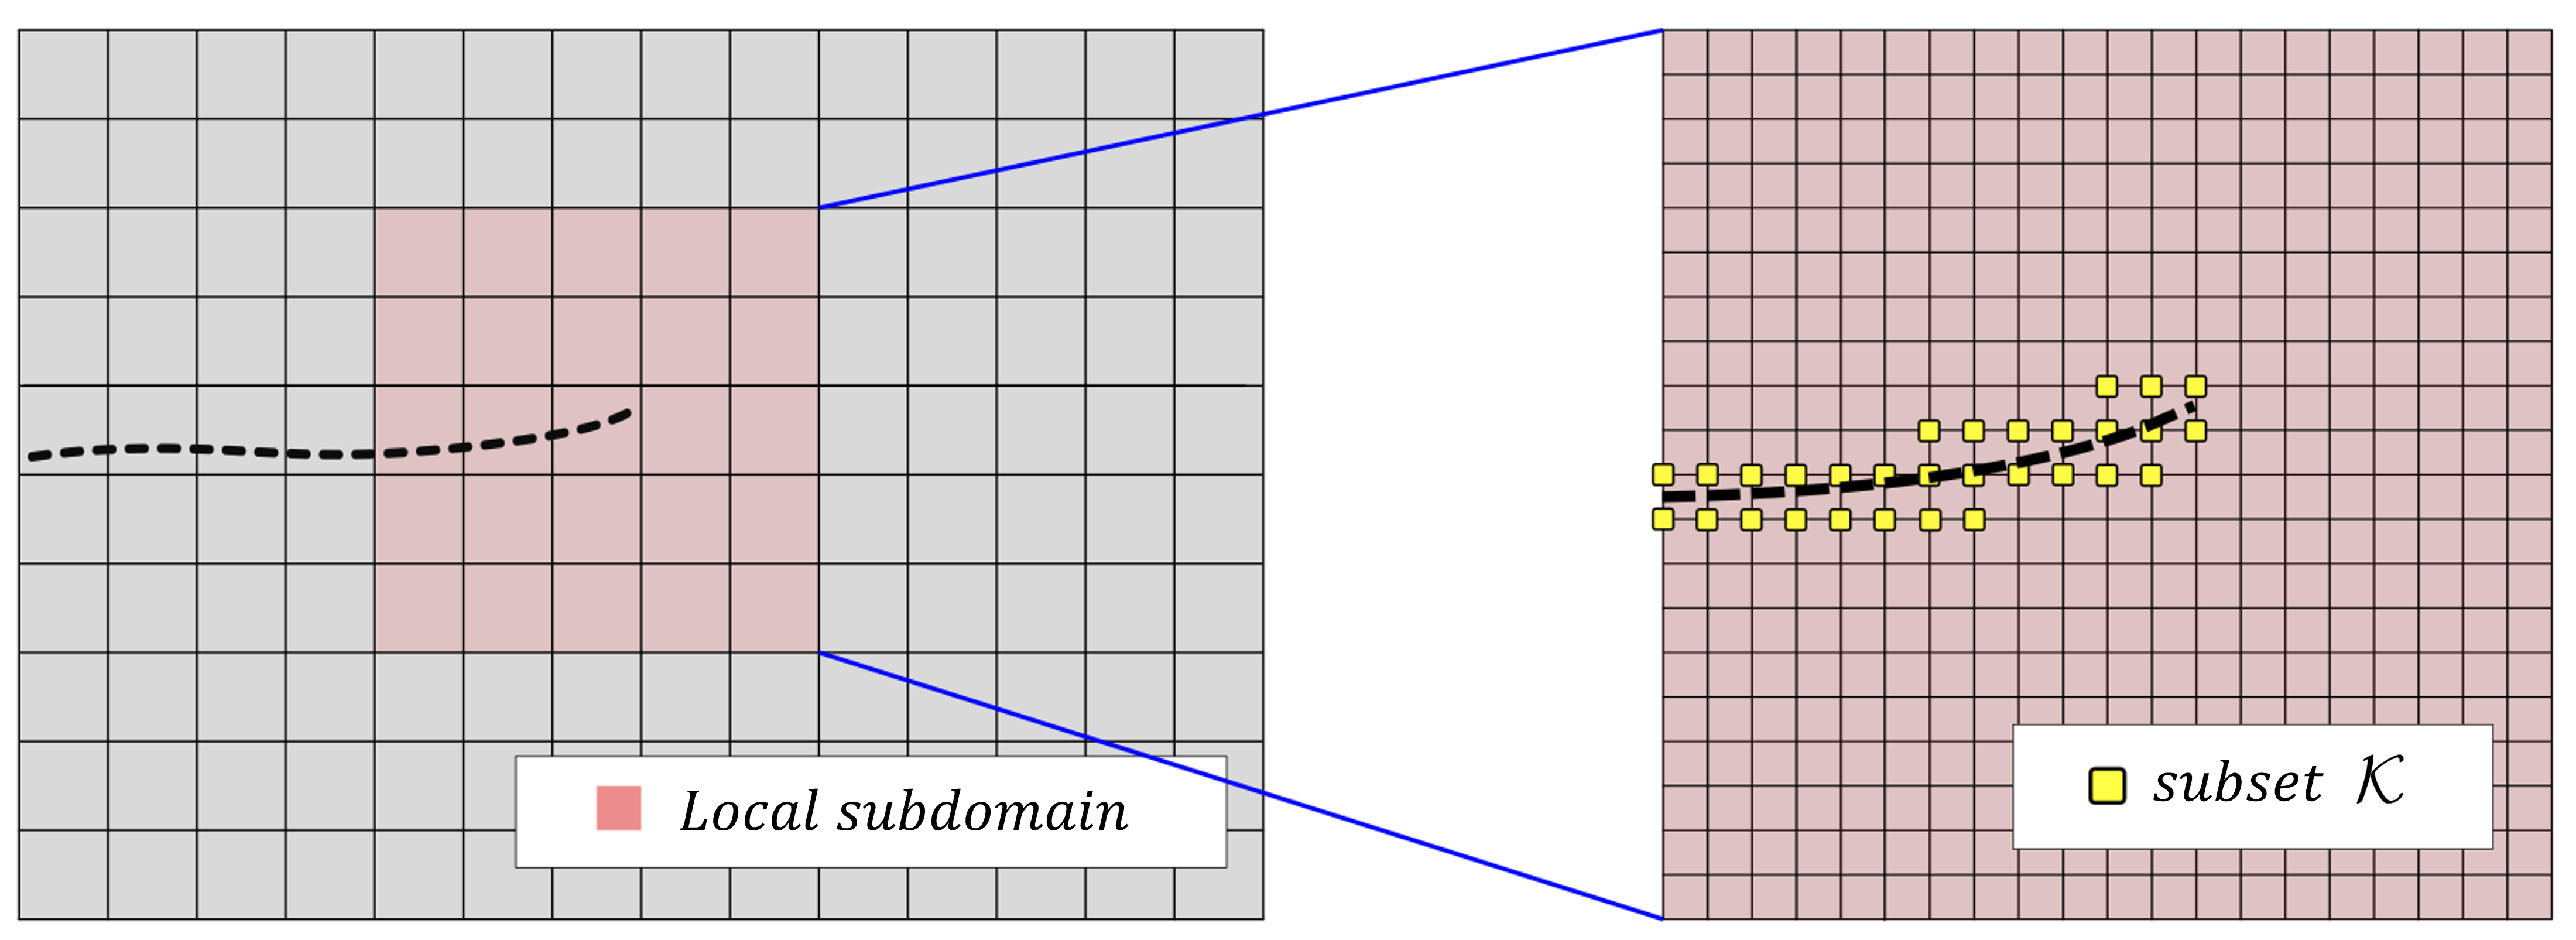
\includegraphics[width=\textwidth]{img/Section2/subset_kappa.png}
    \caption{Global domain $\Omega$ on the left and local domain $\Omega_L$ on the right. The nodes in the subset $\mathcal{K}$, where $d$ is set to $1$ are colored in yellow.}
    \label{fig:subset_kappa}
\end{figure} 

The crack is represented by prescribing $d = 1$ in a set $\mathcal{K} \in \mathcal{T}_L$ of nodes in the local subdomain, as shown in Figure \ref{fig:subset_kappa}. This set is constructed in two steps. First, all elements of $\mathcal{T}_L$ which are intersected by the global fracture triangulation $\mathcal{F}$ are identified.  Then, $\mathcal{K}$ is defined to be the set of all nodes that belong to any of these intersected elements.

\subsubsection{Transfer of global pressures to local mesh}
\label{sec:pressure_projection}

Due to the different levels of resolution between the global and local problems, we find it advantageous to transfer the pressure fields in a particular manner.  We note that in the global problem, the fracture pressures $p_f^h$ are available at the cell centers of 1D finite volumes, and the matrix pressures $p_m^h$ are available at the cell centers of 2D finite volumes.  These fields are transferred to quadrature points in the finite element mesh for the local subproblem using the transfer operators 
$\Pi^{\Omega_L}_f$ and $\Pi^{\Omega_L}_m$.

\begin{figure}[!htbp]
    \centering
    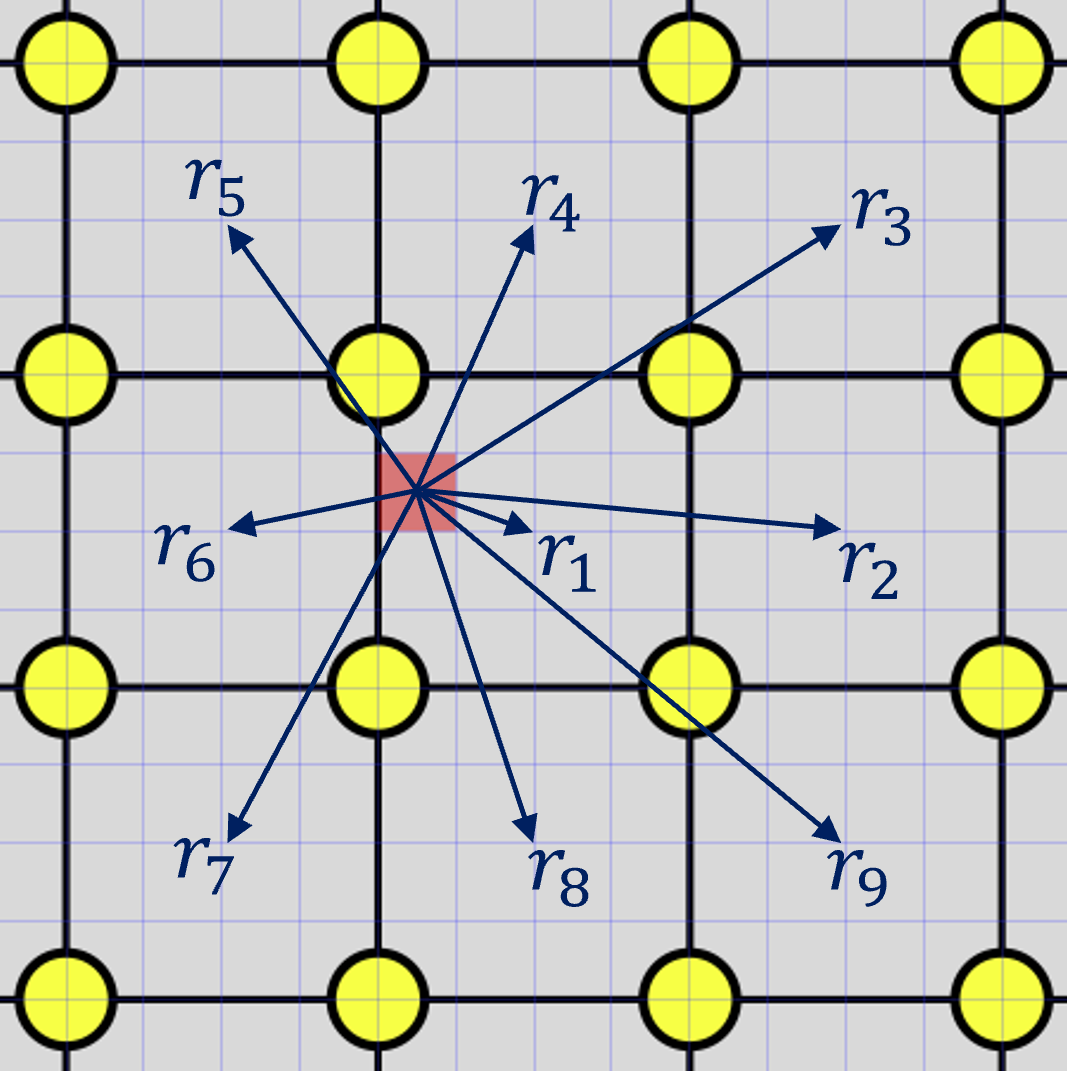
\includegraphics[width=6cm]{img/Section2/pressure_interpolation_blue_small.png}
    \caption{Illustration of global cells (in gray) in the neighborhood of a local element, indicated in pink. The matrix pressure at a quadrature point in the local element is calculated using an average of global pressures from neighboring cells $\{ i \}$, with weights corresponding to the distances $r_i$ between the quadrature point and the cell center.}
    \label{fig:pressure_interpolation}
\end{figure}

The operator $\Pi^{\Omega_L}_f$ that transfers the fracture pressure is straightforward, and inspired by a similar operation described in Santillán et al.\ \cite{santillan2018phase}. Given any point $ {\bf{x}} \in \Omega_L$, and a global fracture pressure field $p_f^h$, $\Pi^{\Omega_L}_fp_f^h({\bf{x}})$ is obtained by finding the closest cell of $\mathcal{F}$ to $x$ and taking the value of $p_f^h$ at this cell. More precisely,

\begin{equation}
    \Pi^{\Omega_L}_f p_f^h({\bf{x}}) = p_f^h(\underset{c \in \mathcal{F}}{\text{arg min }}\text{dist}(c,{\bf{x}} )).
\end{equation}

For the operator $\Pi^{\Omega_L}_m$ that transfers the matrix pressure field, we use an averaging procedure.  This has the effect of smoothing the matrix pressure field at the resolution of the local mesh.  At a quadrature point ${\bf{x}}_Q \in \Omega_L$, the matrix pressure in the local domain is obtained from a weighted average of the pressures in the global cells that surround the point.  Specifically, 
\begin{equation}
    \Pi^{\Omega_L}_m p_m^h({\bf{x}}_Q) = \dfrac{\sum_{i=1}^s r^{-1}_ip_m^h(c_i)}{\sum_{i=1}^s r^{-1}_i},
\end{equation}
where $r_i$ denotes the distance between the quadrature point location and the center of global cell $i$, as indicated in Figure~\ref{fig:pressure_interpolation}.  In the sum, all cells that neighbor the global cell containing quadrature point ${\bf{x}}_Q$ are used.  In the particular case when a quadrature point happens to reside in the center of the local element and $r_1 = 0$, the above sum is replaced with   
$ \Pi^{\Omega_L}_mp_m^h({\bf{x}}_Q) = p^h_m (c_1)$.

\subsection{Local problem discretization}

With the local subdomain properly identified and initialized, we now describe the additional steps to discretize the displacement and damage fields in the local subdomain and solve for their approximations.
The governing equations for the macro-force balance \eqref{basic u problem} and the damage evolution \eqref{damage equation ch3} are both treated with the finite element method.  The damage and displacement fields are both approximated using four-node bilinear quadrilateral elements. 

Let $\Omega_L$ denote the local domain. From the finite-element approximation $\textbf{u}_G^h$ computed in the global problem, we extract $\textbf{u}^h_G|_{\partial\Omega_L}$ and use it to constrain the displacements on the boundary of the subproblem \footnote{In the multi-resolution method of Muixi et al.\ \cite{muixi2021combined},  the displacement boundary conditions near the crack base were released. We did not find this to be necessary in our approach.}.  As such, the trial space $\boldsymbol{\mathcal{U}}^h$ is given by
\begin{equation}\label{disp subspace}
    \boldsymbol{\mathcal{U}}^h = \{ \textbf{u}_L^h \in H^1(\Omega_L)^n \mid \textbf{u}_L^h = \textbf{u}^h_G \text{ on } \partial\Omega_L \}.
\end{equation}

The function space $\mathcal{D}^h$ of admissible damage fields is given by 
\begin{equation}\label{damage subspace}
    \mathcal{D}^h = \{ d^h \in H^1(\Omega_L) \mid d^h = 1 \text{ on } \mathcal{K} \},
\end{equation}
where $\mathcal{K}$ denotes the set of damage-fixed nodes that correspond to the global crack at the beginning of the load step, as described in subsection~\ref{subdomain_construction}. 

The test spaces are given by $\boldsymbol{\mathcal{W}}^h = H_0^1(\Omega_L)^n$ for the displacements and $\mathcal{C}^h = \{ c^h \in H^1(\Omega_L) \mid c^h = 0 \text{ on } \mathcal{K} \}$ for the damage field. The Galerkin approximation to the problem on the local subdomain is then:
\medskip

\begin{mdframed}[
    frametitle={The spatially discrete form},
    frametitlebackgroundcolor=gray!20,
    backgroundcolor=gray!5,
    linewidth=0pt,
    nobreak=true
  ]
  Find $\textbf{u}_L^h \in \boldsymbol{\mathcal{U}}^h$ and $d^h \in \mathcal{D}^h$, such that $\forall \textbf{w}^h \in \boldsymbol{\mathcal{W}}^h$ and $\forall c^h \in \mathcal{C}^h$,
 
 \begin{align}
  \left( \nabla \textbf{w}^h, \boldsymbol\sigma_L^h \right) - \left( \textbf{w}^h, \Pi^{\Omega_L}_f p_f^h \nabla d^h \right) - \left( \textbf{w}^h, \textbf{b} \right) - \left< \textbf{w}^h, \textbf{t} \right>_{\partial_t\Omega} &= 0, \label{eq: semidiscrete momentum balance ch3}   \\
  \begin{split}
    \frac{2G_c^h\ell}{c_0}\left( \nabla c^h, \nabla d^h \right) + \frac{G_c^h}{c_0\ell}\left( c^h, \zeta'(d^h) \right) + \left( c^h, 2(d^h-1)W(\boldsymbol{\epsilon^+}(\textbf{u}_L^h),0) \right) \\
    + \left( c^h, \alpha \Pi^{\Omega_L}_m p_m^h\nabla \cdot \textbf{u}_L^h \right) + \left( \nabla c^h, \Pi^{\Omega_L}_f p_f^h\textbf{u}_L^h \right)  &= 0, \label{eq: semidiscrete damage evolution}    
  \end{split} 
\end{align}

\end{mdframed}
where we have used $(\cdot,\cdot)$ to denote the standard inner product in the $L^2(\Omega)$ space, and $\left< \cdot, \cdot \right>$ to denote its restriction on the boundary.   In the above,  $\boldsymbol\sigma^h_L$ denotes the discrete stress, given by 
\begin{equation}
    \boldsymbol\sigma^h_L = \left( (1-d^h)^2\ \mathbb{C}:\boldsymbol\epsilon(\textbf{u}_L^h) -(1-d^h)\alpha p_m^h \mathbb{I}\right).
\end{equation}

We employ an alternating minimization scheme to solve the coupled system of equations \eqref{eq: semidiscrete momentum balance ch3}-\eqref{eq: semidiscrete damage evolution}. Convergence is measured with respect to the $L_2$-norms of the change in the damage $d^h$ and  displacement fields $\textbf{u}_L^h$, using a relative tolerance of $10^{-4}$. With this approach, each of the equations becomes linear with respect to its primary variable, simplifying the solution process.

We note that \eqref{eq: semidiscrete damage evolution} does not explicitly include the irreversibility constraint  \eqref{eq:ddot-strong}. Within the multi-resolution scheme, the Dirichlet condition $d^h=1$ on the crack set $\mathcal{K}$ is sufficient to prevent the healing of the fracture surface relative to the initial global crack.  It does not, however, enforce irreversibility of the damage throughout the local subdomain, and it is possible that some crack healing could occur if regions are loaded and unloaded during a single time step.  
We did not find this to occur for the problems studied in this work, but it is possible that this could arise in more complex cases and the use of a more robust means of enforcing the constraint on the damage would be needed.  Options include, for example, the active set solver described in \cite{hu2020frictionless}.   

In terms of the local dissipation function $\zeta(d)$, in this work we use $\zeta(d) = d$ which corresponds to the AT-1 phase-field model of fracture.  This is selected due to the fact that it gives rise to a compactly supported damage field and a fully elastic stage prior to damage initiation \cite{pham2011gradient}.
When using the AT-1 model, it is necessary to explicitly enforce the constraint $d^h \ge 0$, as in some cases, this formulation can lead to negative damage values. In this work, this is effected  by invoking a lower threshold on the active part of the strain energy $W(\boldsymbol{\epsilon^+}(\textbf{u}_L^h),0) = 3G_c/8\ell$, as in \cite{miehe2016phase}. 

Finally, we note that phase-field models of fracture tend to give rise to a mesh and regularization length dependent critical fracture energy that is larger than $G_c$ \cite{bourdin2008variational}.  To account for this, we use a discrete value of $G_c^h$ that is obtained as a function of the local mesh spacing and regularization length, as
    \begin{equation}
        G_c^h = G_c \left( 1 + \dfrac{ h_{local} }{c_0\ell} \right)^{-1},
    \end{equation}
such that the effective critical fracture energy is very close to that of the material.  

\subsection{Crack propagation: translating local damage updates into global crack extensions}\label{propagation_step}


A key step of the algorithm concerns how changes to the damage in the local subdomain are translated into updates to the crack geometry in the global domain.  We provide details of our algorithm for this procedure here.  The scheme is presented in the context of a single crack tip that is propagating through the global domain. Although we do not consider much more complex cases in this work, such as changes in crack topology (due to crack branching or merging), we note that such problems have been examined in other works employing hybrid phase-field approaches.  This includes the recent work of Muixi et al.~\cite{muixi2021combined}, albeit in a purely mechanical context.

At each step in the solution algorithm, in the global problem, we keep track of two geometric entities, namely the global crack tip and the global tip element (Figure \ref{fig:all_tips}a). The global crack tip is defined by the interior endpoint of the crack.  The global tip element is the element that contains the tip on one of its sides, but is not yet ``cut" by the crack.  In essence, it is the global element just ahead of the propagating crack tip.   In the local subproblem, we identify a local version of the crack tip that is obtained from the discrete damage field $d^h$ (Figure \ref{fig:all_tips}b and \ref{fig:all_tips}c).  
The algorithm to extend the global crack geometry depends on the relative location of the global crack tip, global tip element, and local crack tip, as described below.

\begin{figure}[!h]
\centering
\begin{subfigure}{.33\textwidth}
  \centering
  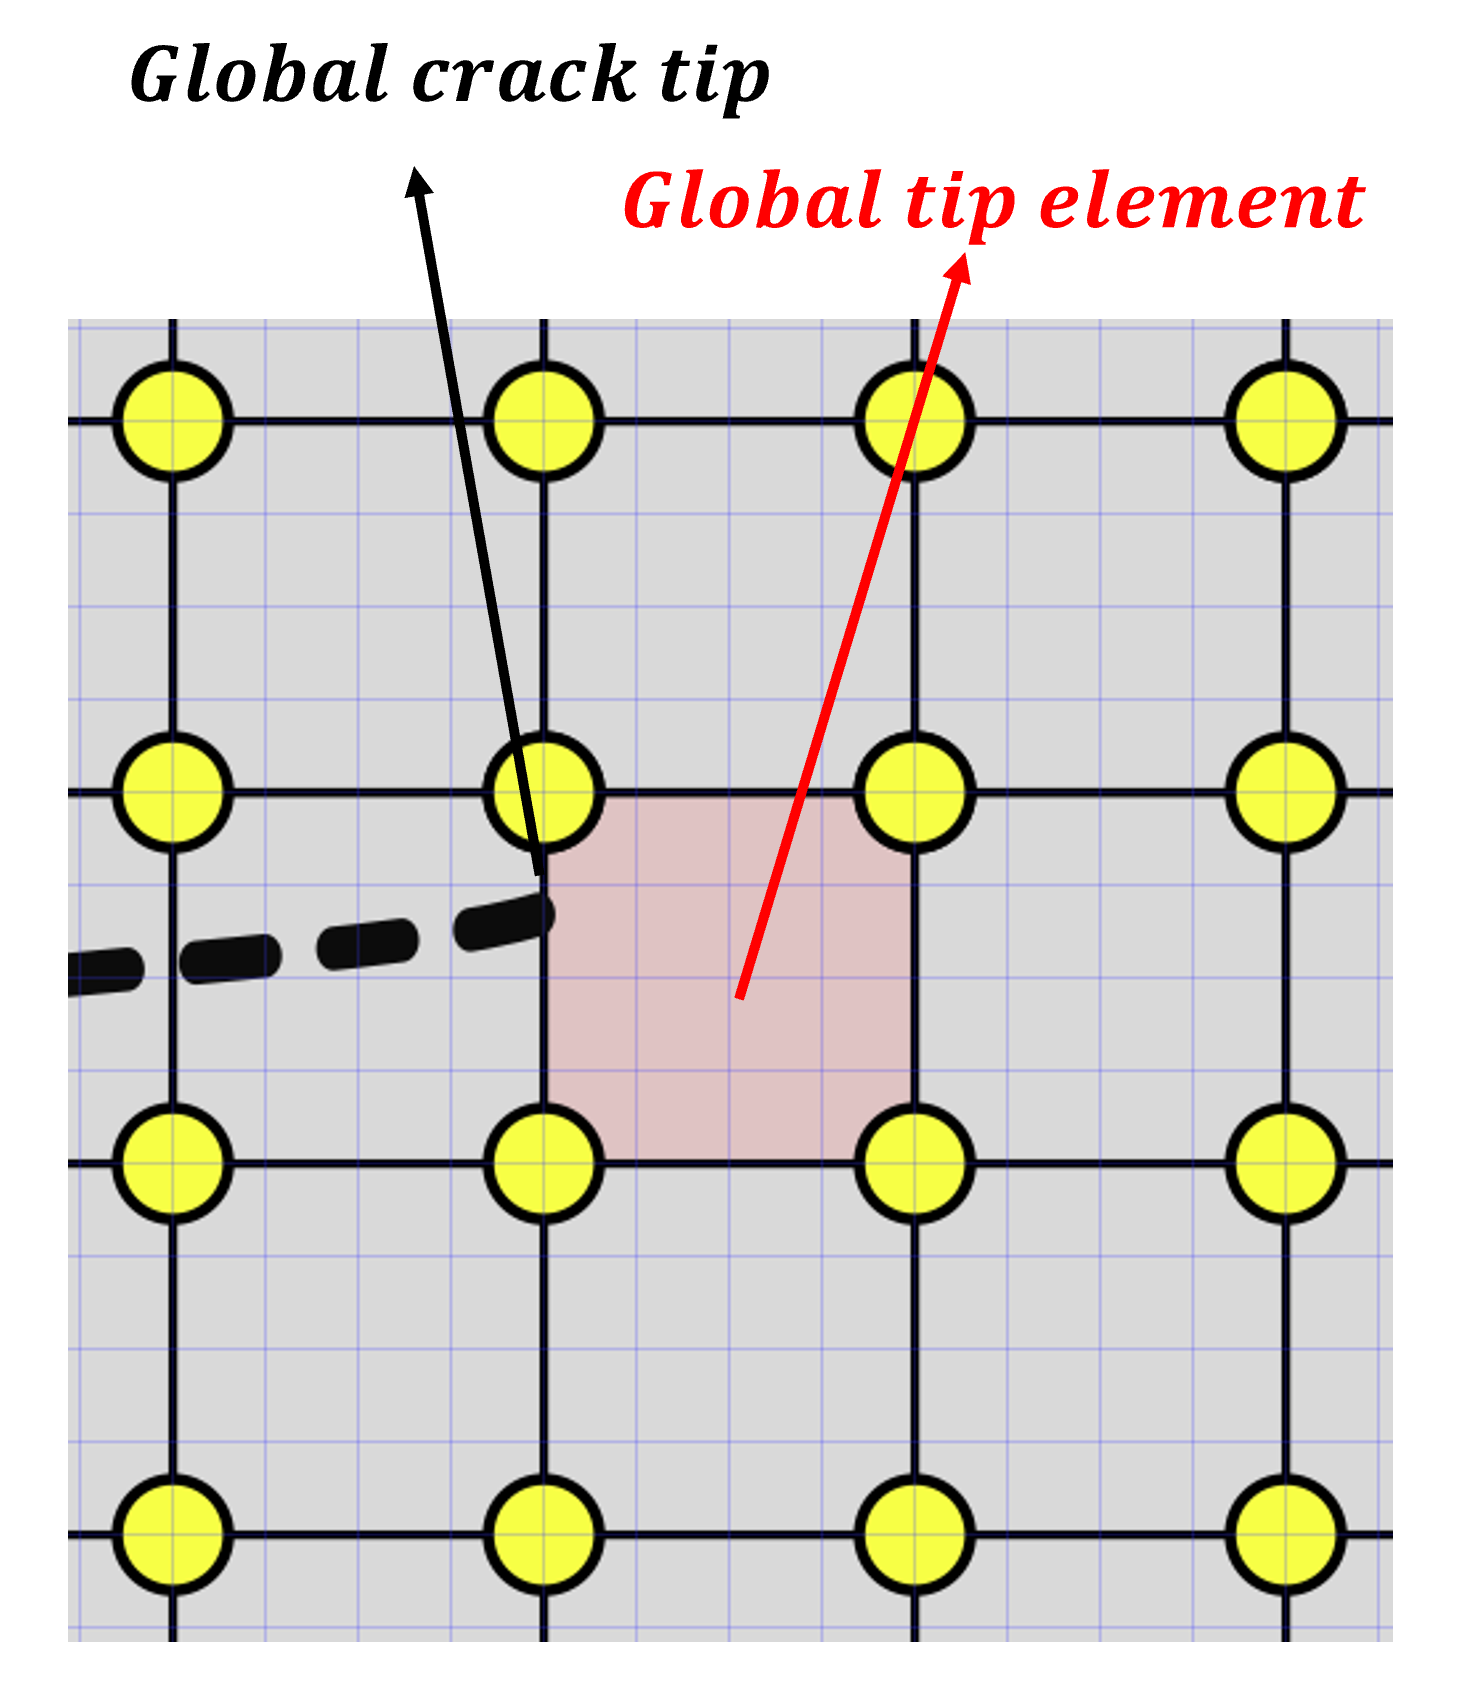
\includegraphics[width=\linewidth]{img/Section2/propagation_items_1.png}
  \caption{}
  \label{fig:prop_items}
\end{subfigure}%
\begin{subfigure}{.33\textwidth}
  \centering
  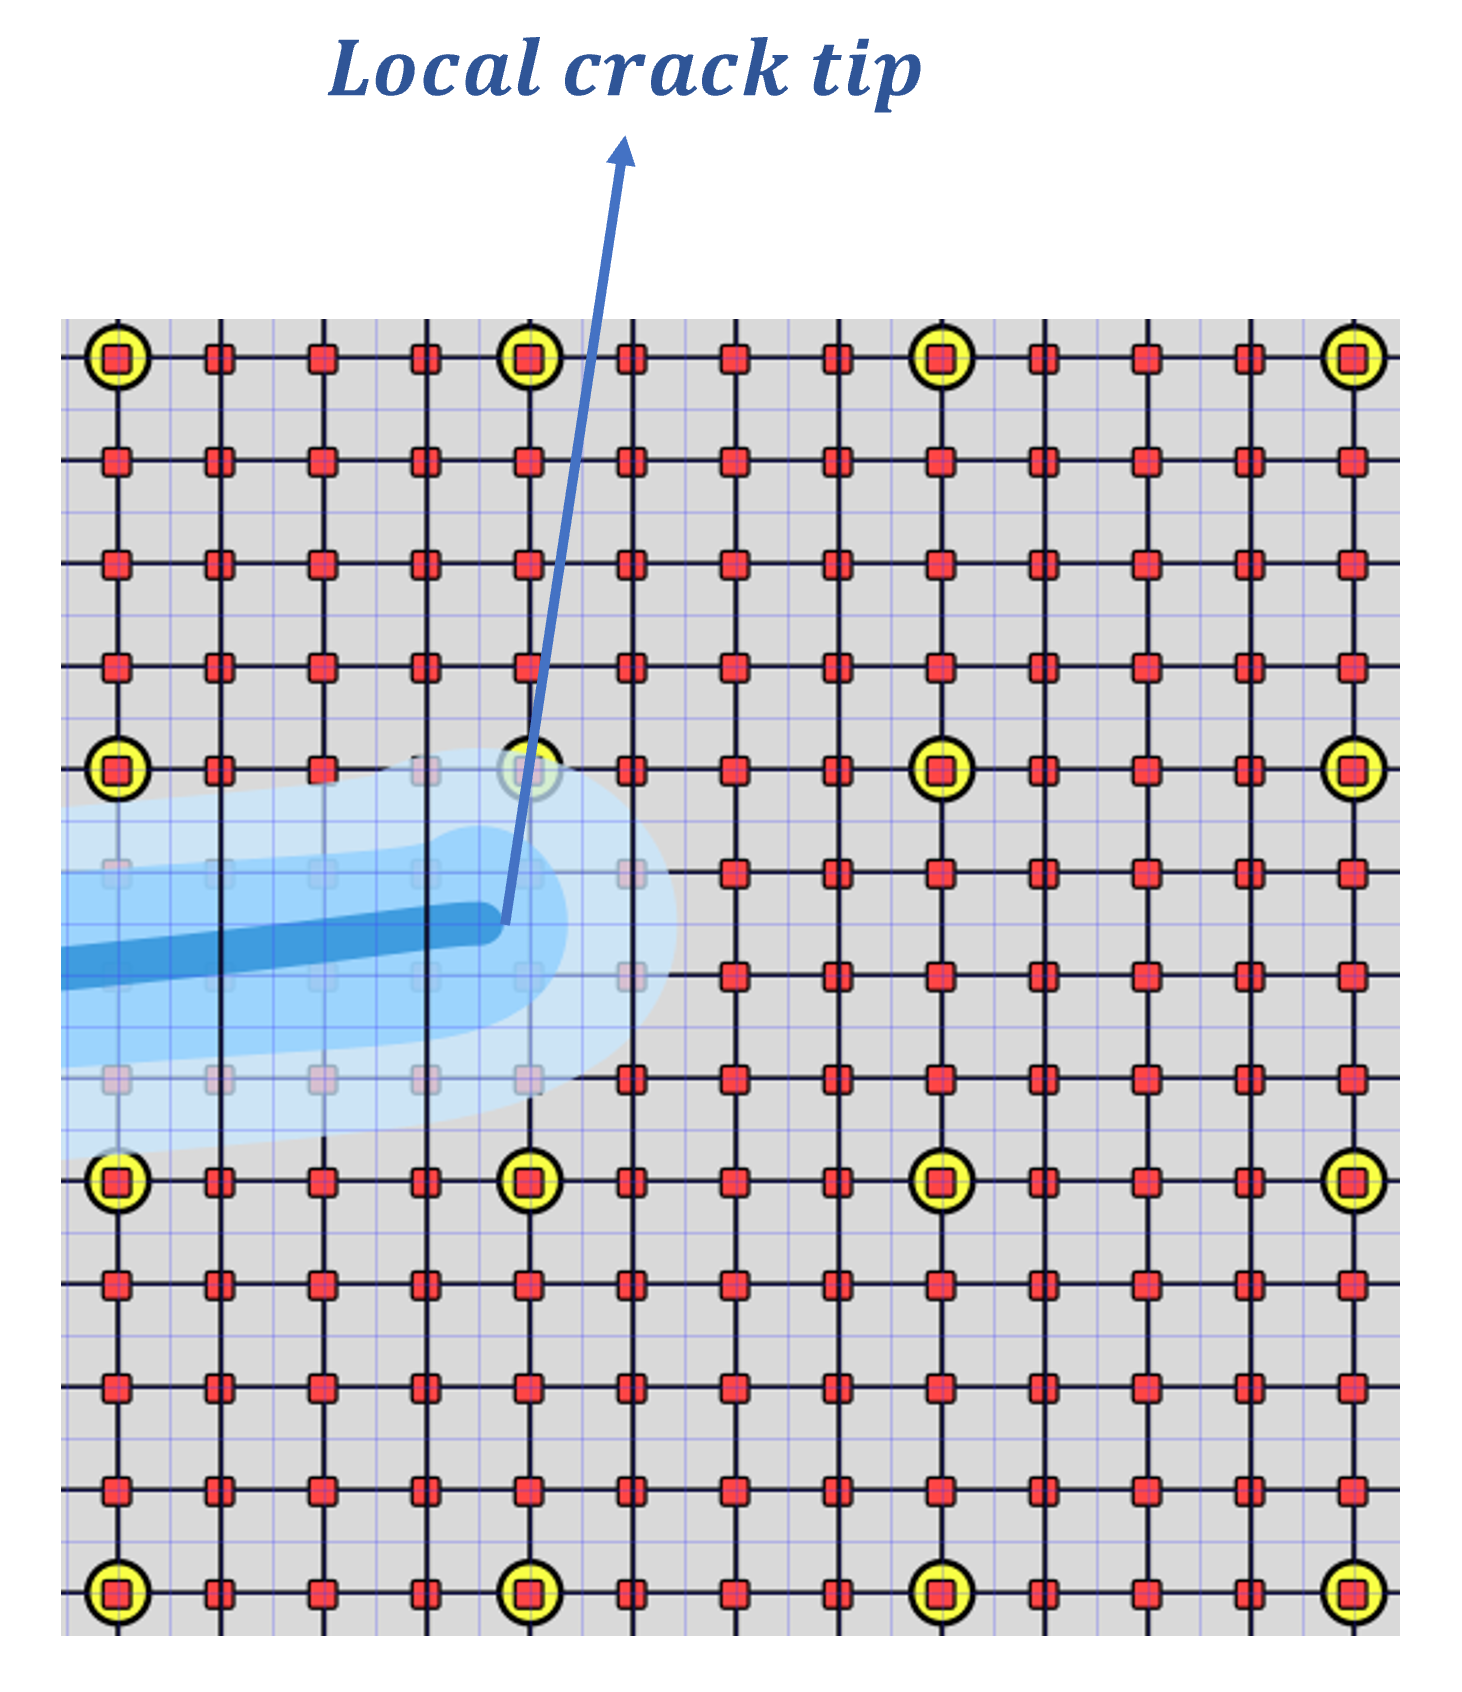
\includegraphics[width=\linewidth]{img/Section2/propagation_items_2.png}
  \caption{}
  \label{fig:prop_items2}
\end{subfigure}
\begin{subfigure}{.33\textwidth}
  \centering
  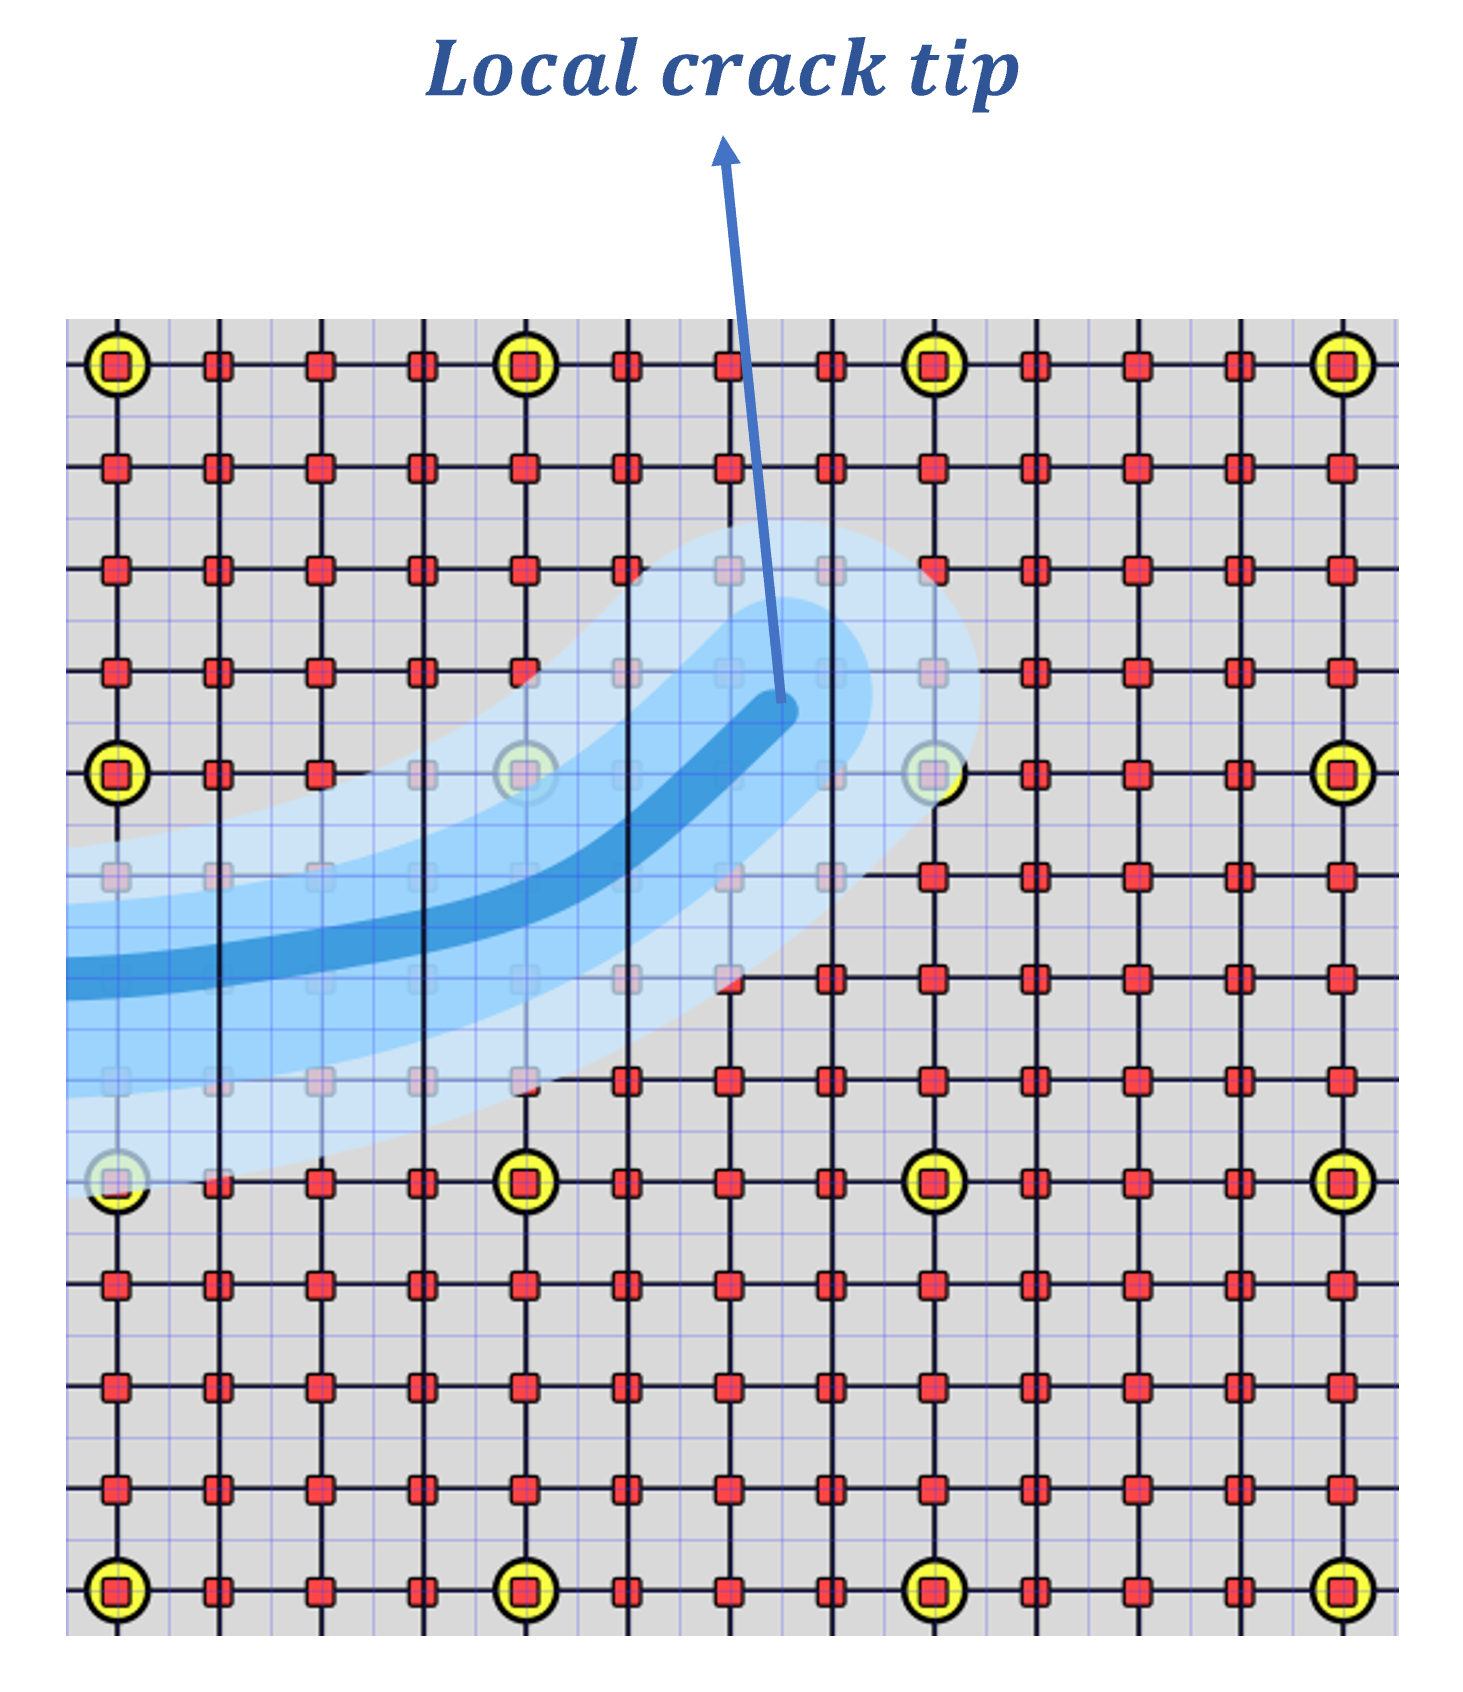
\includegraphics[width=\linewidth]{img/Section2/propagation_items_3.png}
  \caption{}
  \label{fig:prop_items3}
\end{subfigure}
\caption{(a): Illustration of the global crack tip and global tip element. (b) Case when the local tip falls inside the tip element. (c) Case when the local tip falls outside the tip element.}
  \label{fig:all_tips}
\end{figure}

The enrichment strategy described in Section~\ref{sec:global_disc} requires global elements that are completely cut by the crack geometry.  As such, any extension of the crack geometry at the global scale must correspond to the global tip element being fractured.  Accordingly, global crack propagation is triggered whenever the local tip falls outside the tip element. In this case, the new global tip is identified by connecting the current global tip and the local tip. Since the local tip is outside the tip element, a new segment will intersect the perimeter of the tip element exactly once (neglecting the obvious intersection at the current global tip). This process is illustrated in Figure \ref{fig:tip_progression}. Any crack advance beyond this new tip location is neglected at this point, and the algorithm returns to a new global solve with an updated crack geometry.  

\begin{figure}
\centering
\begin{subfigure}{.331\textwidth}
  \centering
  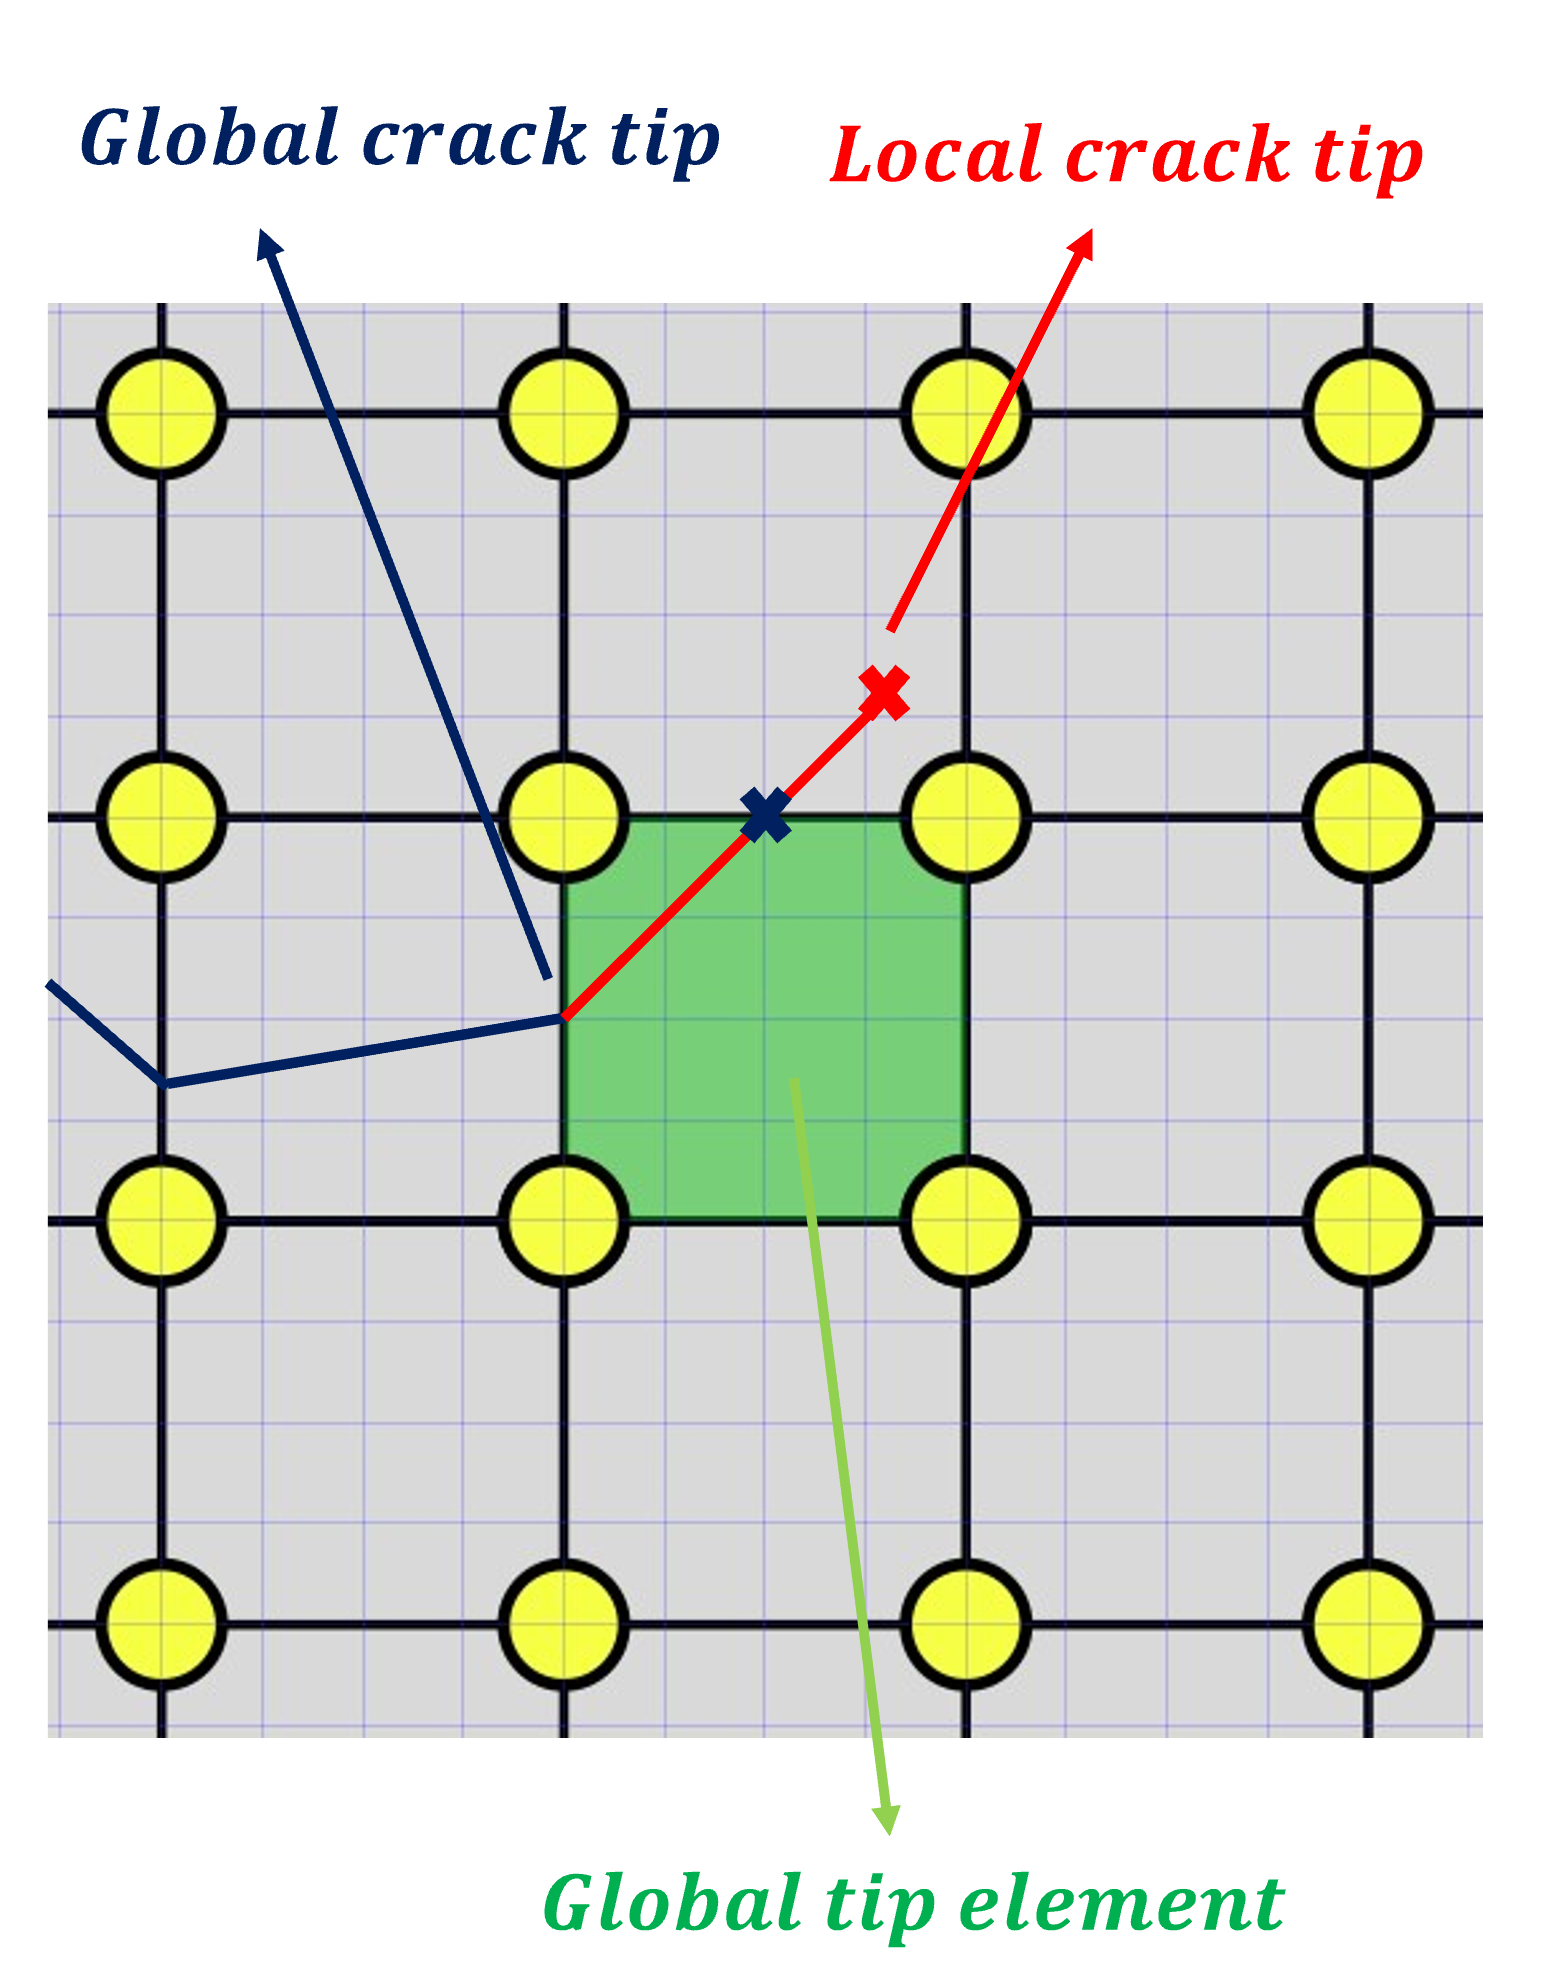
\includegraphics[width=.99\linewidth]{img/Section2/schematic_1.png}
  \caption{}
  \label{fig:prop_1}
\end{subfigure}%
\begin{subfigure}{.33\textwidth}
  \centering
  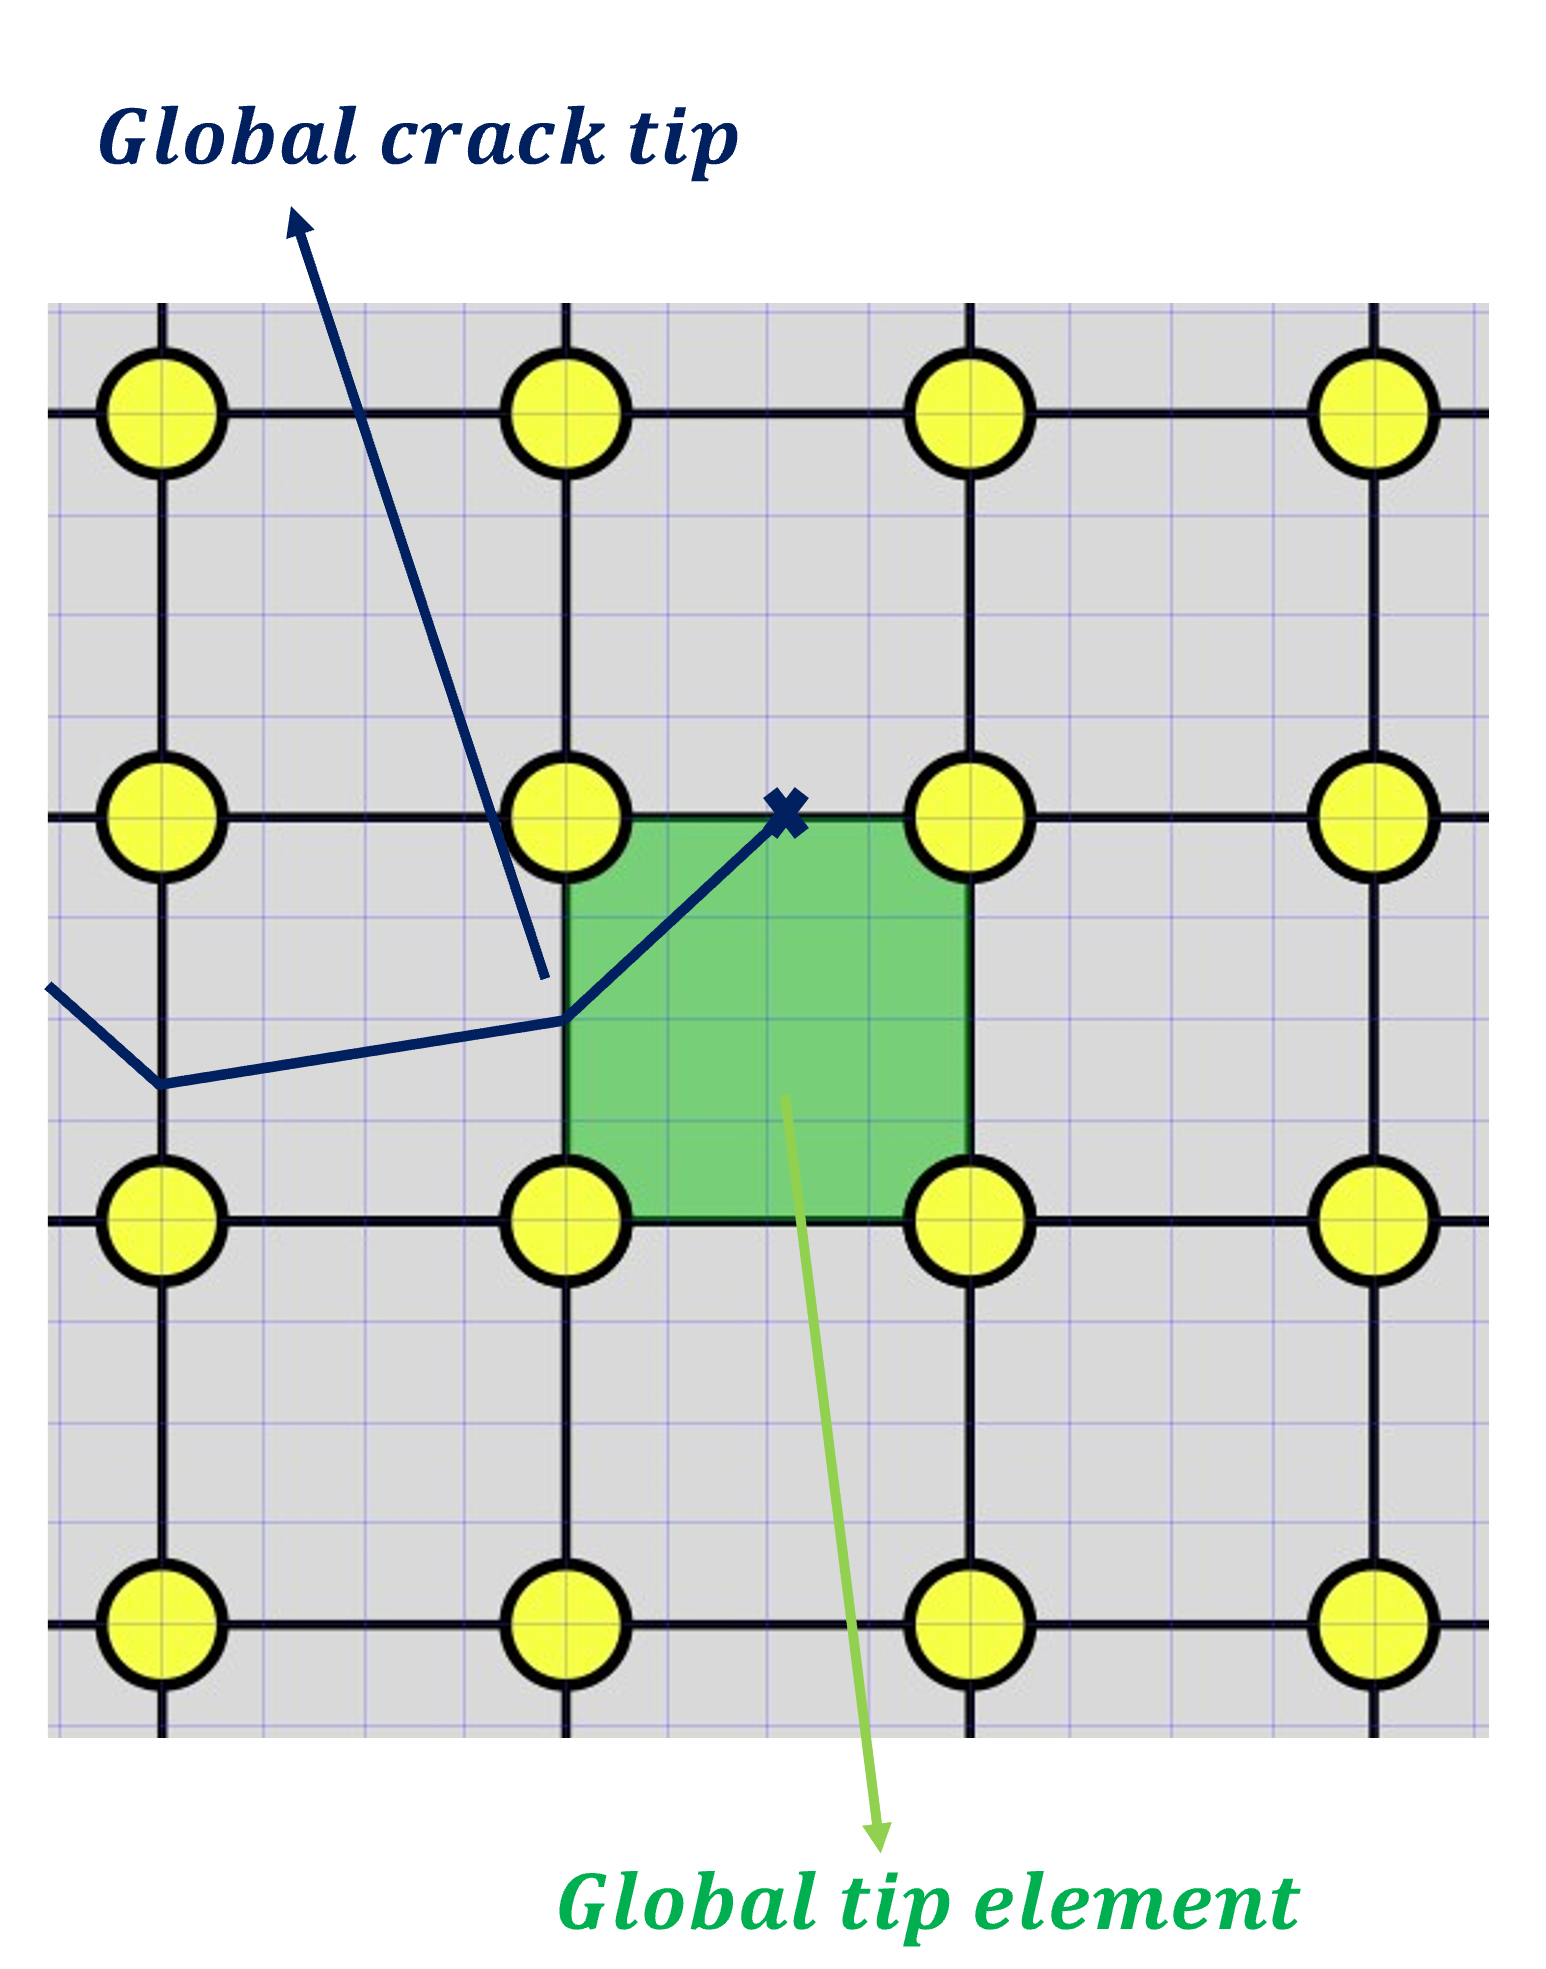
\includegraphics[width=\linewidth]{img/Section2/schematic_2.png}
  \caption{}
  \label{fig:prop_2}
\end{subfigure}
\begin{subfigure}{.33\textwidth}
  \centering
  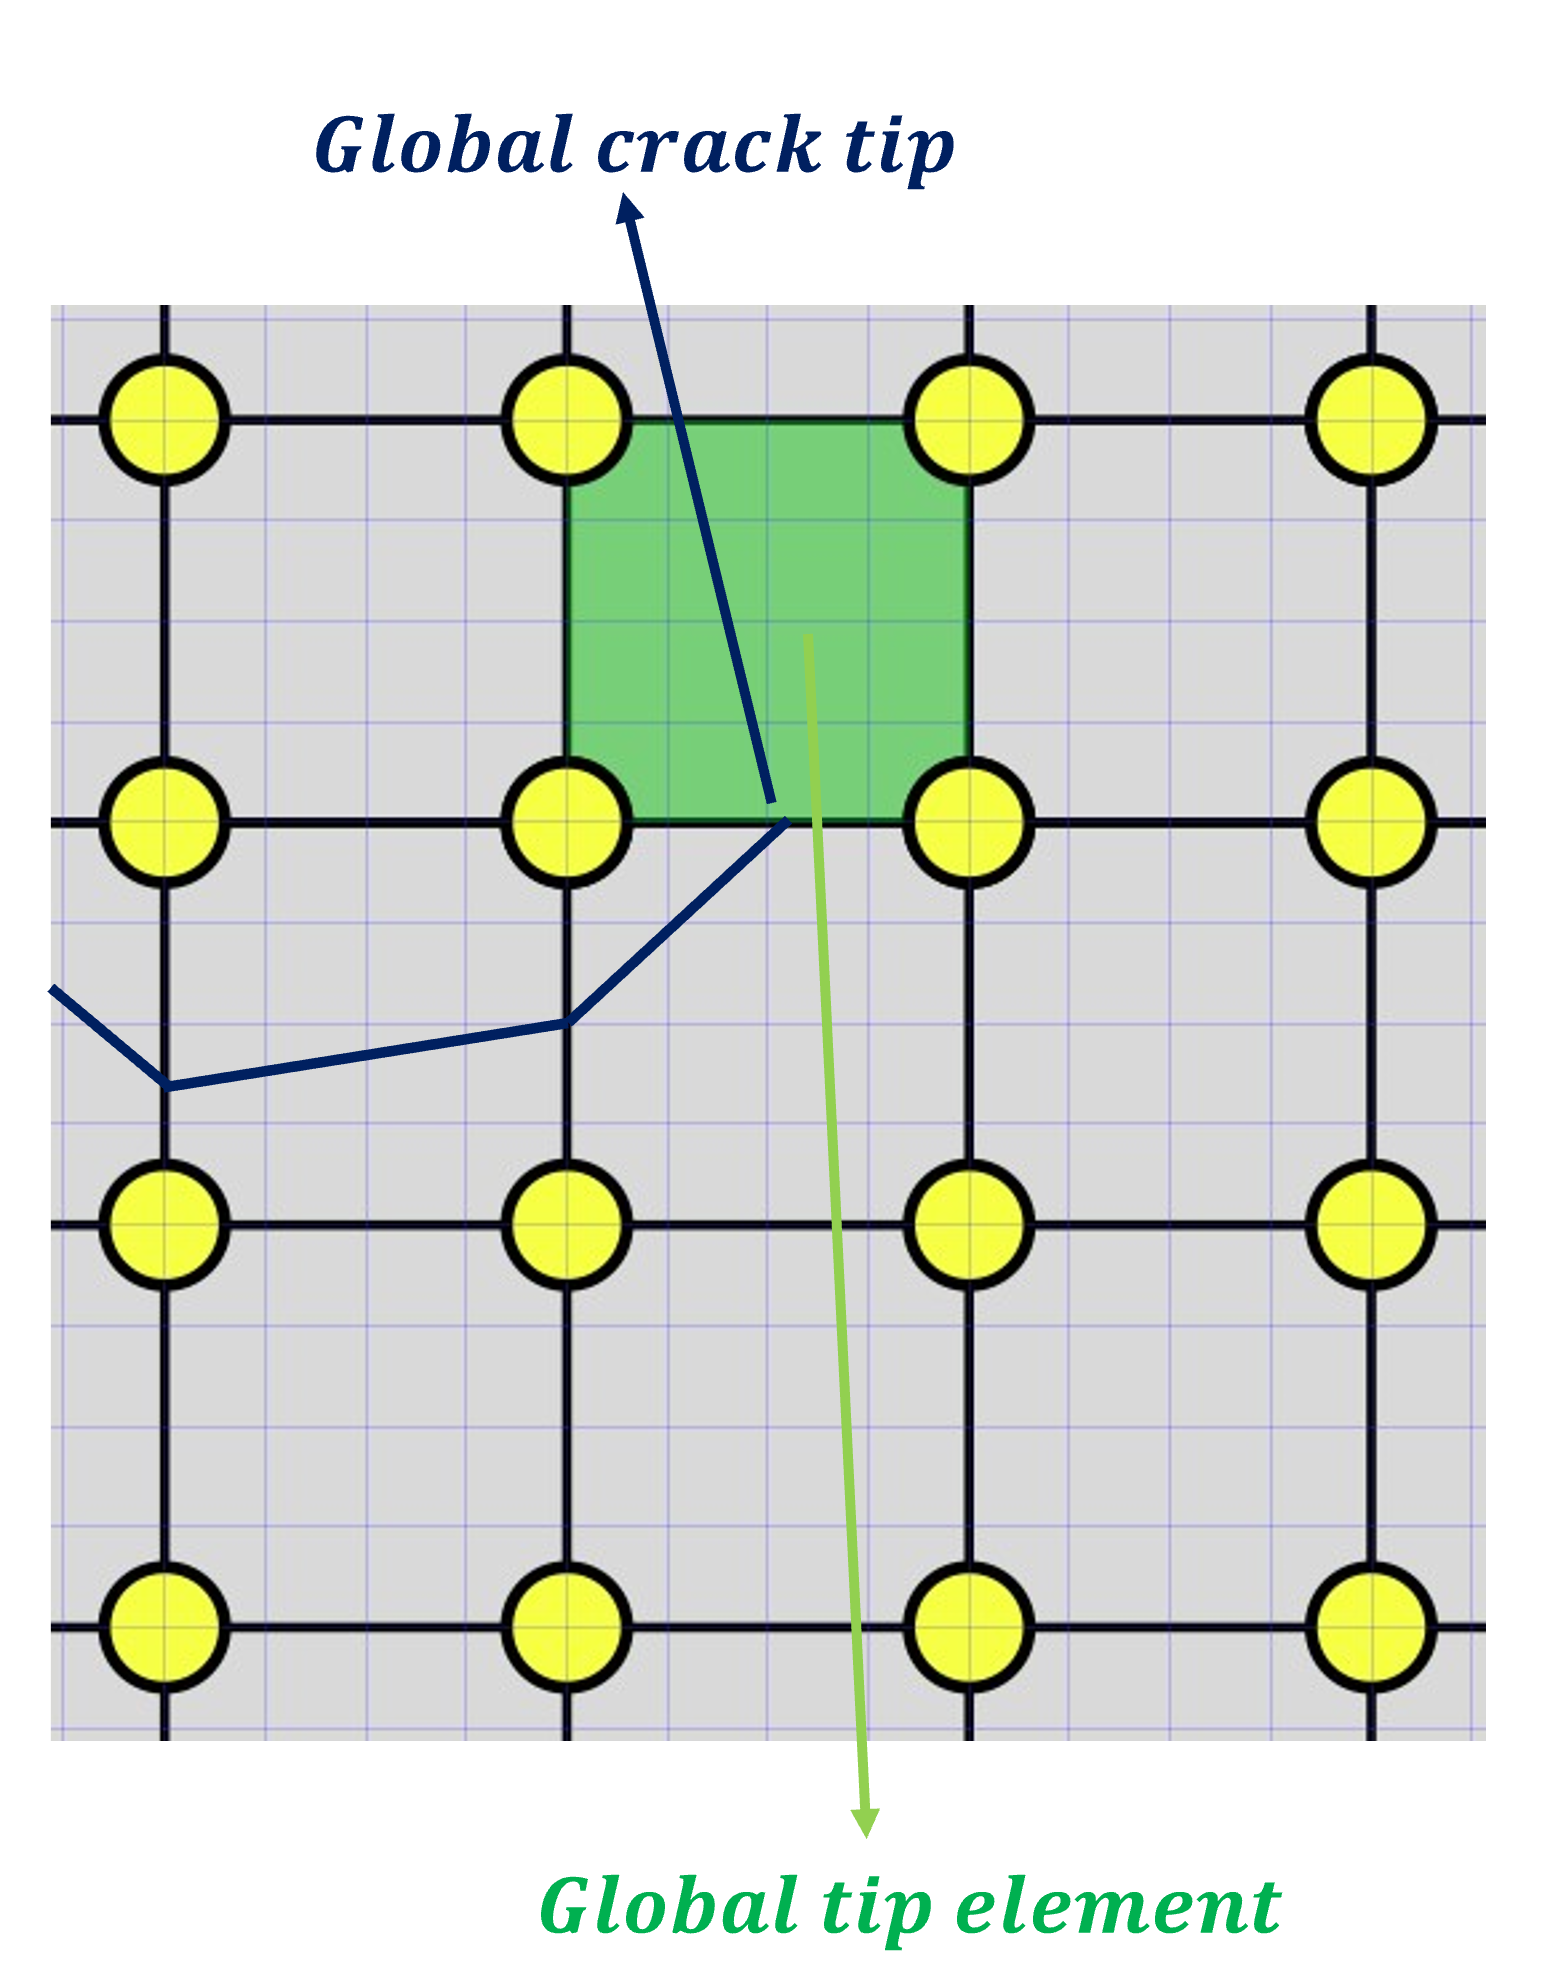
\includegraphics[width=\linewidth]{img/Section2/schematic_3.png}
  \caption{}
  \label{fig:prop_3}
\end{subfigure}
\caption{(a): Construction of the segment connecting global and local tips.  (b) New crack segment to be added. (c) Update of the global crack tip and global tip element.}
  \label{fig:tip_progression}
\end{figure}

In general, the problem of extracting a sharp crack front from a diffuse representation is not trivial. When the crack evolution involves complex topological changes, it is particularly difficult\cite{tamayo2015medial}. In the numerical examples studied in this manuscript, we take advantage of the relatively simple fracture geometry and predicted crack patterns to simplify this process.  In particular, we first identify all elements in the local subdomain with nodes whose damage values are all above a threshold $d_{tr}$. A similar approach was proposed in \cite{giovanardi2017hybrid}. The local crack tip is taken to be the center of the element in this set that is farthest from the base of the crack in the local subdomain.  The threshold used for this process is taken to be $d_{tr} = 1 - h_{local}/(2\ell)$, which is based on the estimate for a damage field near a crack tip given in \cite{yoshioka2020crack}. In essence, for a phase-field model of fracture, this threshold identifies nodes that are expected to correspond to the peaks of the discrete damage field.  For a damage band resolved with a mesh spacing of $\ell / h_{local} = 4$, this gives rise to a threshold of  $d_{tr} = 0.875$. 

\subsection{Algorithm summary}

Having described the solution strategies for both the global and local problems and the transfer of various quantities, we now detail the algorithm \eqref{mr_algorithm} that couples the two problems together to simulate crack propagation. Figure~\ref{fig:solution_algorithm} provides an illustration of the algorithm. Within each time step (outer loop), the algorithm employs an inner loop that allows the global problem to be updated as soon as any large enough change in the crack geometry is detected in the local subproblem.  The inner loop is terminated when the propagation step, described in subsection \ref{propagation_step} does not identify any crack advance.  The construction with two nested loops can be viewed as an implicit treatment of the fracture front position, which, according to Lecampion et al.\ \cite{lecampion2018numerical} tends to be more accurate and robust, permitting the use of larger time steps.

\medskip

\begin{algorithm}[H]\label{mr_algorithm}
\small
\SetAlgoLined
 Define initial and boundary conditions
 
 $n = 1$ \\
 $n_F = endStep$
 
 \While{$n \le n_F$}{
 
    \medskip
    
    $\mathcal{F}_n^{1} = \mathcal{F}_{n-1}$
 
    \For{$1 \le k \le maxIter\footnote{The index $k$ is only a dummy variable for this loop that searches for the correct fracture geometry at a given time step.}$}{

    \medskip
    
    (1) Solve \textbf{Global Problem} and obtain $\textbf{u}_G^{k,n}, p_m^{k,n}, p_f^{k,n}$

    \medskip
    
    (2) Construct subdomain $\Omega_L$ and submesh $\mathcal{T}_L$. Identify subset of cracked nodes $\mathcal{K}$.
    
    \medskip
    
    (3) Prescribe local boundary conditions $\textbf{u}^h_{L}|_{\partial\Omega_L} = \textbf{u}_G^{k,n}|_{\partial\Omega_L}$ and $d^h = 1$ on $\mathcal{K}$.
    
    \medskip
    
    (4) Construct local pressure fields $p_m= \Pi^{\Omega_L}_m (p_m^{k,n})$ and $p_f = \Pi^{\Omega_L}_f (p_f^{k,n})$
    
    \medskip

    (5) Solve the \textbf{Local Problem} to obtain $d^{k}$.

    \medskip
    
    (6) Use $d^{k}$ and the propagation step (subsection \ref{propagation_step}) to update discrete fracture $\mathcal{F}_n^{k}$.

    \medskip
    
    \If {$\mathcal{F}_n^{k+1}$ = $\mathcal{F}_n^{k}$}{
    
        \medskip
    
        n = n + 1
        
        \medskip
        
        $\mathcal{F}_n = \mathcal{F}_n^{k}$
        
        \medskip
            
        $\textbf{u}_G^n = \textbf{u}_G^{k,n}$
        
        \medskip
            
        $p_m^n = p_m^{k,n}$
        
        \medskip
        
        $p_f^n = p_f^{k,n}$
        
        \medskip
            
        break
        
        \medskip
    
        }

    }
    
 }
 \caption{Solution algorithm for multi-resolution hydraulic fracture}
\end{algorithm}

\begin{figure}[h]
    \centering
    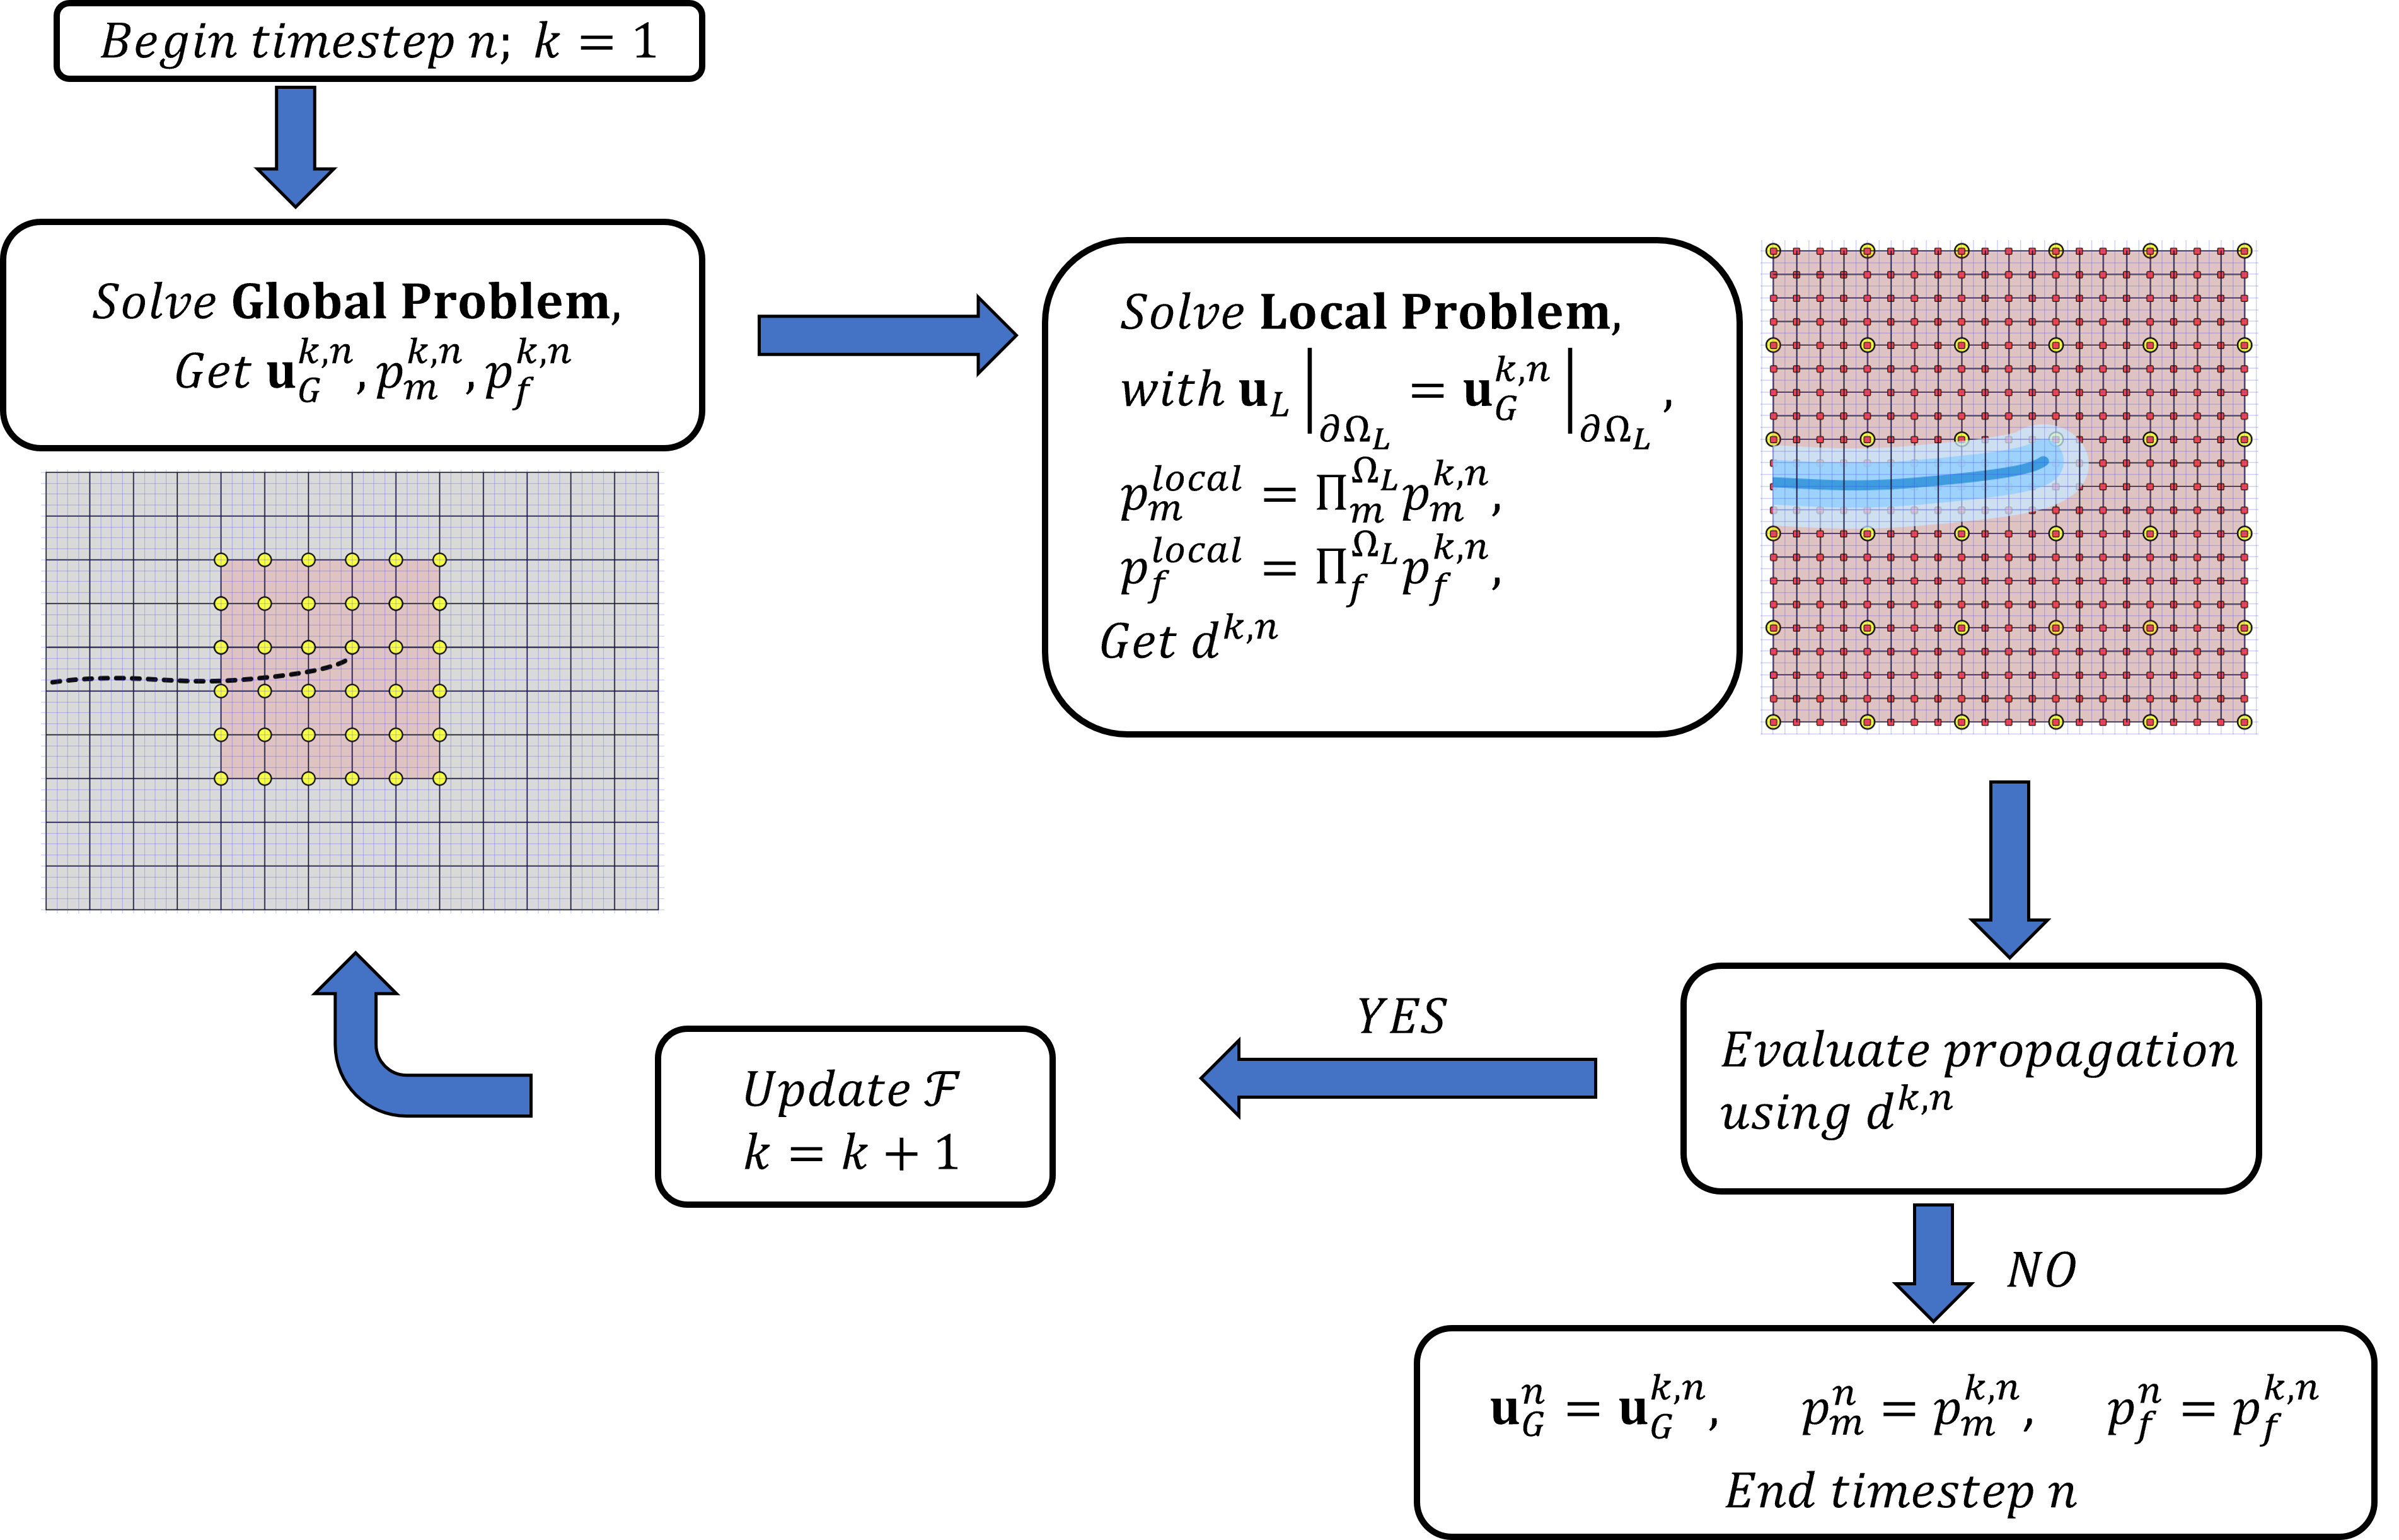
\includegraphics[width=\linewidth]{img/Section2/algorithm_fancy.png}
    \caption{Multi-resolution solution algorithm.}
    \label{fig:solution_algorithm}
\end{figure}



\newpage 

\section{Numerical Results}\label{results_section}

We now present the results from various benchmark problems in fluid-driven fracture propagation.  The problems range from those in which flow is only present within the cracks to fully coupled problems involving flow in both the matrix and the evolving manifold that is the fracture geometry. With the sole exception of the toughness-dominated KGD problem,  all of the results in this section employ the spectral split of the energy, as described in Section~\ref{sec:pfm-fracture}.  

\begin{figure}[!htbp]
\centering
\begin{subfigure}{.5\textwidth}
  \centering
  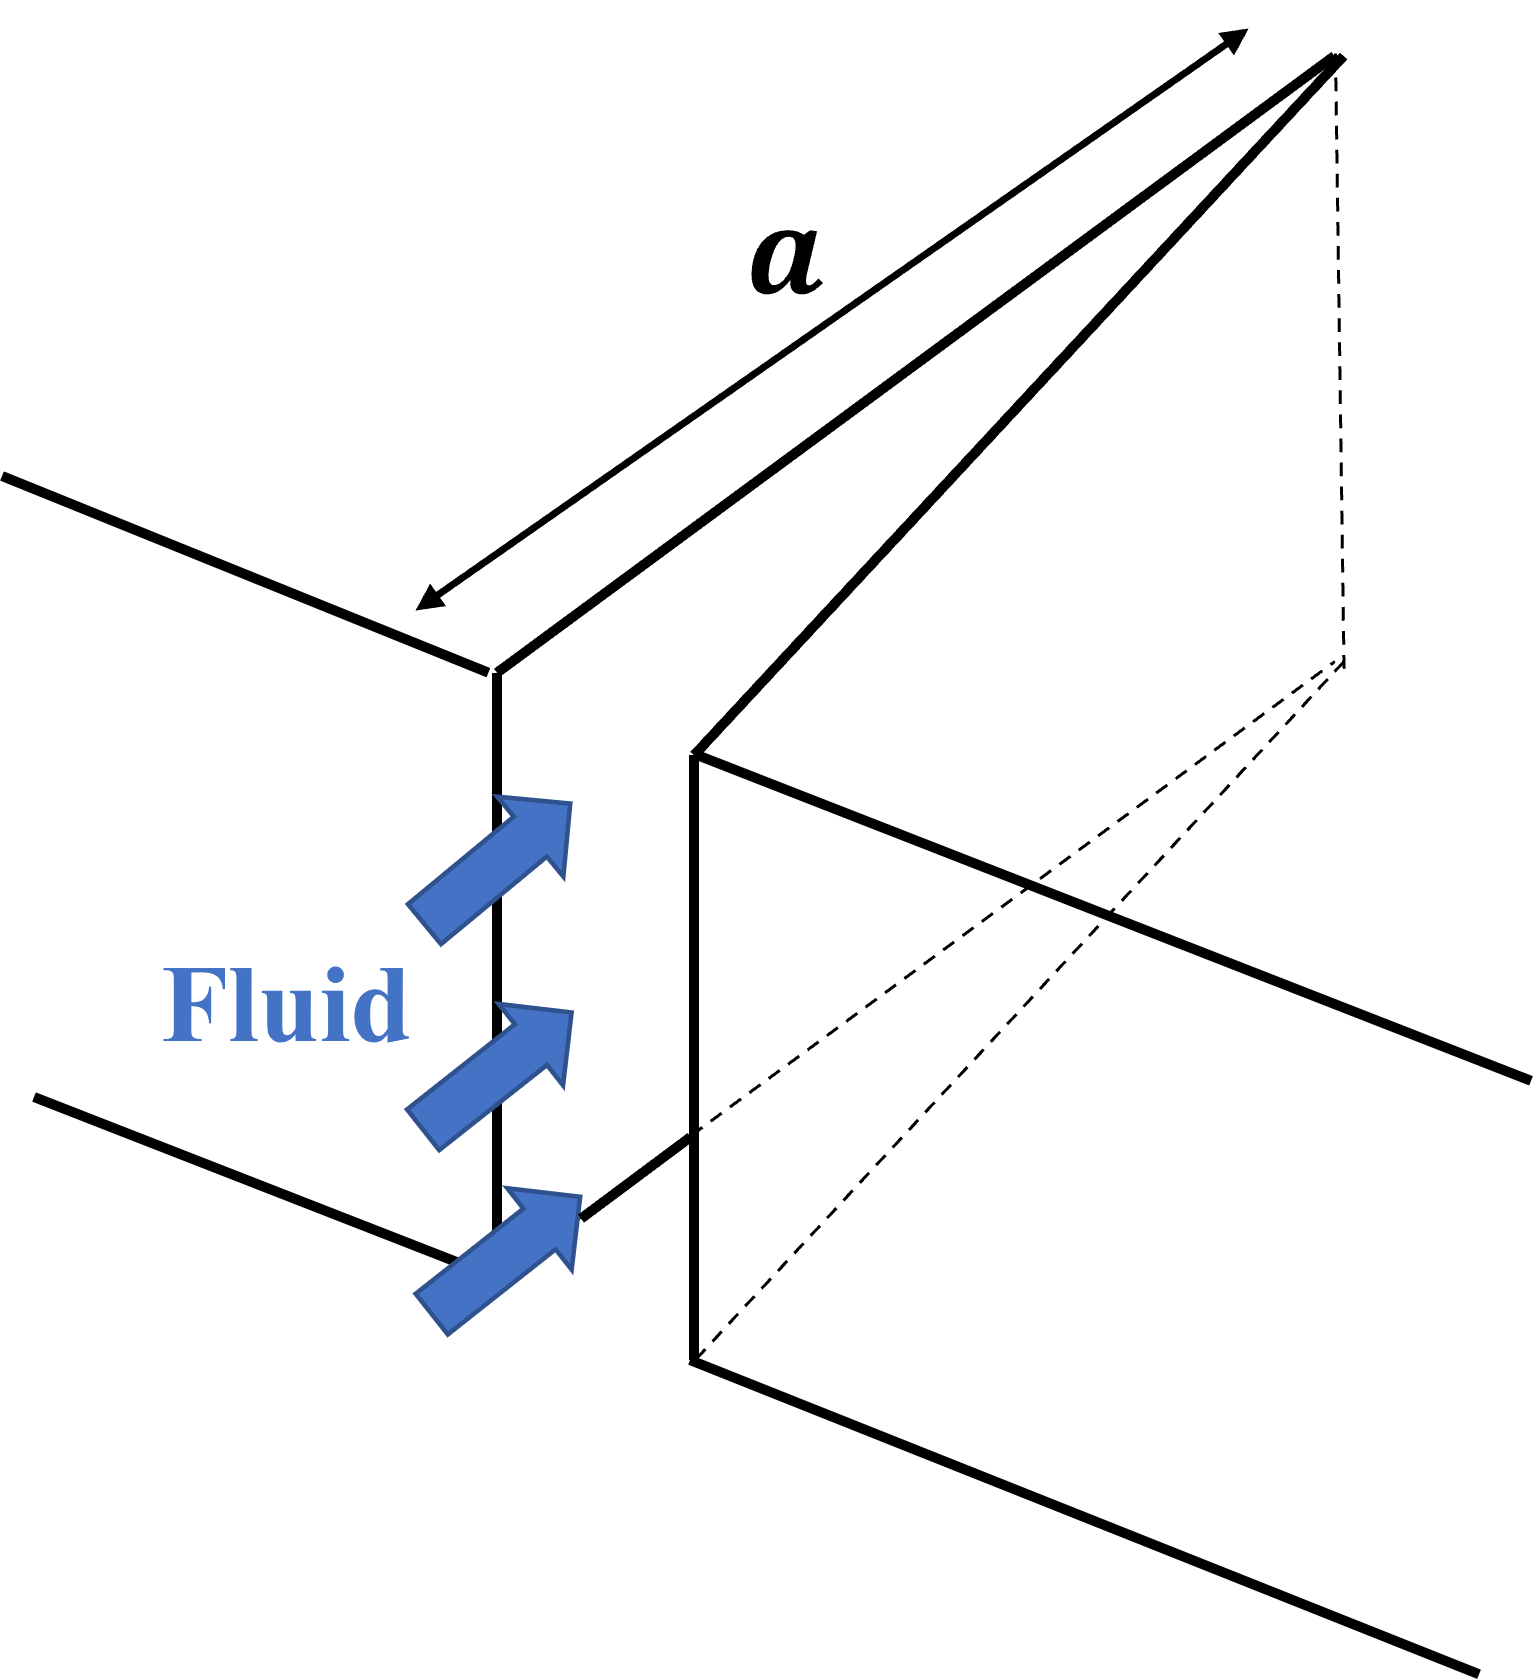
\includegraphics[width=.79\linewidth]{img/KGD_schematic_mine.png}
    \caption{}
    \label{fig:3D_schematics_kgd}
\end{subfigure}%
\begin{subfigure}{.5\textwidth}
  \centering
  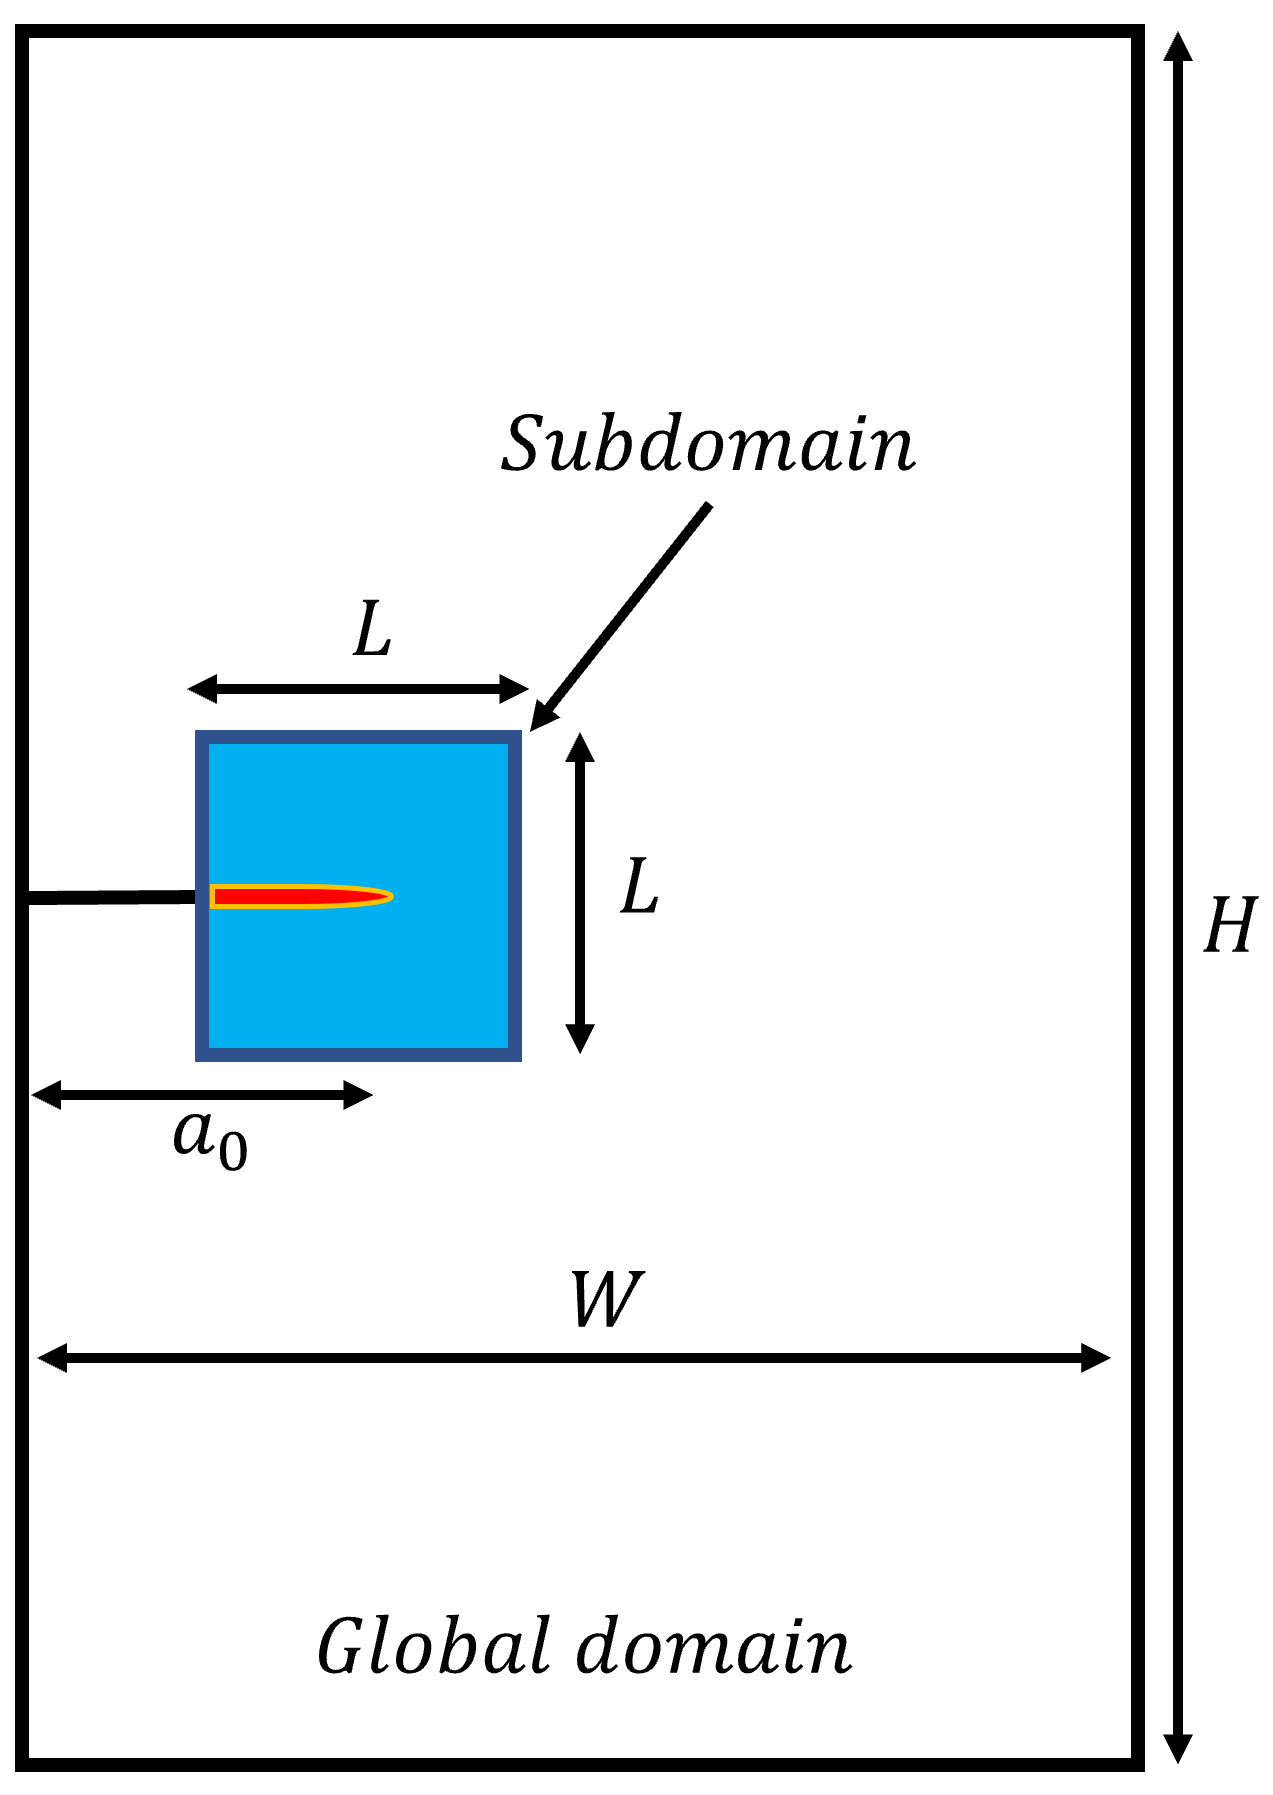
\includegraphics[width=.62\linewidth]{img/toughness_prob/KGD_schematic_2.png}
  \caption{}
  \label{fig:2D_schematics_kgd}
\end{subfigure}
\caption{(a) Schematic of the KGD problem, inspired by \cite{adachi2007computer}. (b) Computational domain for the KGD problem (not to scale).}
  \label{fig:kgd_schematics}
\end{figure}

\subsection{KGD problems} 
We begin with the well-known Khristianovic, Geertsma and De Klerk (KGD) problems of hydraulic fracture \cite{geertsma1969rapid, zheltov19553}.  The problems concern the propagation of a planar fracture in an infinite, impermeable domain, under the injection of a viscous fluid at a constant rate (Figure \ref{fig:kgd_schematics}). 

The response of the system can be characterized by the dimensionless group $\mathcal{K}$ \cite{detournay2016mechanics}:
\begin{equation}\label{KGD_group}
    \mathcal{K} = \dfrac{4G^{1/2}_{c}}{(6\pi^2E'Q\mu)^{1/4}},
\end{equation}
where $E' = E/(1-\nu^2)$. Values of $\mathcal{K} > 4$ correspond to the ``toughness dominated regime" in which crack growth is largely controlled by the fracture toughness of the media.  By contrast, when  $\mathcal{K} < 1$, the fracture toughness is relatively small and the fluid viscosity is the main factor controlling the speed of crack growth.  In the following, we explore the performance of the multi-resolution algorithm to simulate problems in both regimes.  

\subsubsection{Toughness-dominated regime}
The toughness dominated regime is characterized by the creation of new fracture surfaces accounting for almost all of the energy dissipation.  
In this scenario, the fluid can be considered to be inviscid, which leads to a constant pressure distribution over the entire crack.  The assumption of inviscid flow reduces much of the complexity, allowing for the construction of a simple analytical solution for this problem. 
Here, we consider a problem in the toughness-dominated regime resulting from the material parameters and settings given in Table \ref{parameters_tKGD}.  Using these values in \eqref{KGD_group}, we obtain $\mathcal{K} = 6.54$. 

\begin{table}[ht]
\centering
\caption{Material properties and problem parameters for the toughness-dominated KGD problem}
\begin{tabular}[t]{lcc}
\hline
&Value &Unit \\
\hline
Young's modulus ($E$)&16.0&GPa\\
Poisson's ratio ($\nu$)&0.18&--\\
Fluid viscosity ($\mu$)&1.0$\times10^{-12}$&$\text{GPa . s}$\\
Energy release rate ($G_c$)&1.85$\times10^{3}$&$\text{N/m}$\\
Injection rate ($Q$)&1.0$\times10^{-3}$&$\text{m}^2/\text{s}$\\
Initial crack size ($a_0$) &4&$\text{m}$\\
\hline
\end{tabular}
\label{parameters_tKGD}
\end{table}%

The analytical solution for this problem can be separated into two stages as a function of time. 
In the first stage, the pressure builds linearly with time and the crack does not propagate, as the pressure is below the critical threshold $p_{cr} =(G_cE'/\pi a_0)^{1/2}$.  The pressure then reaches the critical value at $t=t_{cr}$, after which the crack begins to propagate. In the second stage the propagation is stable, since the amount of fluid injected is finite and crack propagation leads to a pressure drop as the total space available for the fluid to occupy increases.

The solution for the crack length and pressure in the crack can be written as

\begin{equation}\label{length_solution_tkgd}
    a(t) =     \begin{cases}
      a_0, &  t \le t_{cr},  \\
      \left(\dfrac{E'(Qt)^2}{\pi G_c}\right)^{1/3}, &  t \ge t_{cr}, 
    \end{cases}
\end{equation}

\begin{equation}\label{pressure_solution_tkgd}
    p(t) =     \begin{cases}
      \dfrac{t}{t_{cr}}p_{cr}, &  \ t \le t_{cr},\\
      \left(\dfrac{E'G_c^2}{\pi Qt}\right)^{1/3}, &  t \ge t_{cr},
    \end{cases}
\end{equation}

\noindent where $t_{cr} =(\pi G_c a_0^3/Q^2E')^{1/2}$. A derivation of this solution can be found in Yoshioka \cite{yoshioka2020crack}.

For simulations using the multi-resolution scheme, a computational domain of size $W\times H = 30\text{ m} \times 240\text{ m}$ is used (Figure \ref{fig:2D_schematics_kgd}). According to \cite{isida1973analysis}, this domain size should be sufficiently large to yield a good approximation to an infinite plane.  We first report results using a sub-domain size of $L \times L = a_0 \times a_0$.   The sensitivity of the results to the choice of sub-domain size will be discussed later in this subsection.  

In what follows, we report results from a refinement study.  In particular, we report results for three different regularization lengths of decreasing value, beginning with $\ell = a_0/15$.  As the regularization length is decreased, we maintain a mesh size in the subdomain of $h_{local} = \ell/{4}$.  This allows the finite-element approximation to sufficiently resolve the regularized fracture band. We also note that the effective fracture toughness in the computational problem depends on $h/\ell$ \cite{yoshioka2020crack}.  In the global domain, we maintain the mesh spacing at the ratio of $h_{global} = 3h_{local}$.  For the coarsest global mesh, this translates into roughly 20 elements over the span of the initial crack geometry.  This level of resolution is consistent with those found to be sufficient for resolving pressurized cracks using the Embedded Finite Element Method, in Cusini et al.\ \cite{cusini2021simulation}.

The results obtained with the multi-resolution scheme are compared to the analytical solutions \ref{length_solution_tkgd} and \ref{pressure_solution_tkgd} in Figures \ref{fig:tkgd_length} and \ref{fig:tkgd_pressure}. We note the overall good match between the simulation results and the analytical solution, as well as the convergence of the results towards \ref{length_solution_tkgd} and \ref{pressure_solution_tkgd} when $\ell$ decreases. Although this problem is relatively simple as the matrix is assumed to be impermeable, it does test the coupling between the global and the local domains and verifies that the phase-field method, even when used only in a vicinity of the crack tip, can still provide accurate predictions of fracture propagation. Although the spectral split was not employed for this problem, we did examine the results using it.  Qualitatively they were found to be very similar, with slightly less accuracy in the calculated values of the critical pressure.   

\begin{figure}
\centering
\begin{subfigure}{.5\textwidth}
  \centering
  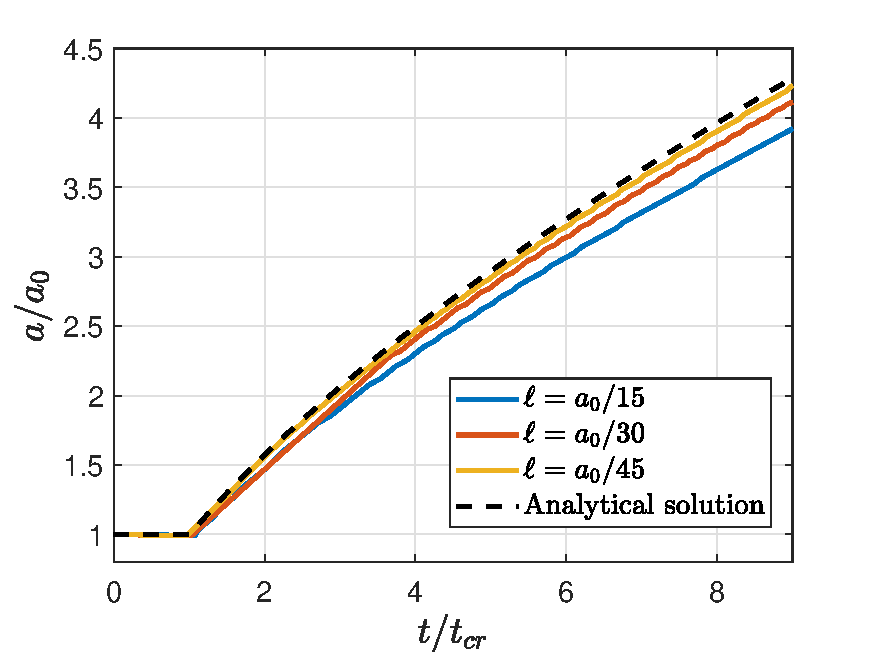
\includegraphics[width=.99\linewidth]{img/toughness_prob/length_tkgd}
  \caption{}
  \label{fig:tkgd_length}
\end{subfigure}%
\begin{subfigure}{.5\textwidth}
  \centering
  \includegraphics[width=.99\linewidth]{img/toughness_prob/pressure_tkgd}
  \caption{}
  \label{fig:tkgd_pressure}
\end{subfigure}
\caption{Comparison of numerical results and analytical solution for the toughness-dominated KGD problem: (a) crack length vs.\ time and (b) pressure vs.\ time.}
  \label{fig:tkgd_charts}
\end{figure}
\FloatBarrier

We now examine the sensitivity of the results to changes in the subdomain size.  This is accomplished by fixing the sizes of the global and local meshes as well as the regularization length, and varying only $L$ in Figure \ref{fig:2D_schematics_kgd}. In particular, we fix the regularization length to $\ell = 0.13\text{ m}$ and vary the sub-domain size between $15\ell$ and $45\ell$.  

Figures \ref{fig:adjusting_L_a} and \ref{fig:adjusting_L_p} provide the results for the pressure and crack length as a function of time, for the various choices of subdomain size. Table \ref{subdomain_size_table} shows the error in the computation of the crack length relative to the analytical solution.  The error is taken as an average over the time range, starting at the beginning of propagation.

\begin{figure}[!htbp]
\centering
\begin{subfigure}{.5\textwidth}
  \centering
  \includegraphics[width=\linewidth]{img/toughness_prob/length_L_analysis}
  \caption{}
  \label{fig:adjusting_L_a}
\end{subfigure}%
\begin{subfigure}{.5\textwidth}
  \centering
  \includegraphics[width=\linewidth]{img/toughness_prob/pressure_L_analysis}
  \caption{}
  \label{fig:adjusting_L_p}
\end{subfigure}
  \caption{Study of the effects of subdomain size on the results of the toughness-dominated KGD problem:  (a) influence on predicted crack length and (b) predicted pressure. }
  \label{fig:adjusting_L}
\end{figure}
\FloatBarrier

\begin{table}[ht]
\centering
\caption{Effect of subdomain size on the relative error in the crack length. }
\begin{tabular}[t]{lcccc}
\hline
Subdomain size &Relative error   \\
\hline
$L = 15\ell$&11.5\%&\\
$L = 30\ell$&3.3\%&\\
$L = 45\ell$&1.1\%&\\

\hline
\end{tabular}
\label{subdomain_size_table}
\end{table}%

The results indicate that the error reduces as the subdomain size is increased.  In this particular study, both the global and subdomain meshes are fairly refined, and so the improvement in accuracy as $L$ increases is not likely due simply to better resolution in the local subdomain.  Rather, it may be due to the fact that the two problems are coupled through the global displacements applied to the subdomain boundary.  As the subdomain size is increased, the boundary of the subdomain moves farther from the crack tip singularity, and one would expect a better correspondence between the displacement fields obtained from the global problem and those obtained using a phase-field approximation over the entire domain.  Furthermore, as the global displacements are held fixed until the regularized crack advances sufficiently far, there is some sensitivity of the proximity of the regularized crack tip to the subdomain boundary.  

In more general cases, one would expect the subdomain mesh to be at quite a bit higher resolution than the global mesh. Since the phase-field problem also requires several iterations in the alternate minimization scheme, problems are expected to become much more computationally expensive as $L$ is increased. As a result, a trade-off between accuracy and computational cost is to be expected.  In general, one should select  a subdomain size that strikes a balance between being large enough to capture the crack evolution and small enough to render the overall calculation efficient. 

\subsubsection{Viscosity dominated KGD problem}

We now consider a case in which the choice of parameters gives rise to conditions wherein the energy dissipation is dominated by viscous dissipation.  In particular, we consider the material properties and problem parameters provided in Table~\ref{parameters_vKGD}.  Consistent with \eqref{KGD_group}, these values give rise to $\mathcal{K} = 0.57$, a result that is clearly within the viscosity-dominated regime.   

\begin{table}[ht]
\centering
\caption{Material properties and problem parameters for the viscosity-dominated KGD problem}
\begin{tabular}[t]{lcc}
\hline
&Value &Unit \\
\hline
Young's modulus ($E$)&0.17&GPa\\
Poisson's ratio ($\nu$)&0.20&--\\
Fluid viscosity ($\mu$)&1.0$\times10^{-10}$&$\text{GPa . s}$\\
Energy release rate ($G_c$)&21&$\text{N/m}$\\
Injection rate ($Q$)&1.0$\times10^{-3}$&$\text{m}^2/\text{s}$\\
Initial crack size ($a_0$) &4.0&$\text{m}$\\
\hline
\end{tabular}
\label{parameters_vKGD}
\end{table}%

In this scenario, the toughness of the medium can be neglected, and the fracture evolution is effectively dictated by the motion of the fluid front.  In this case, the pressure varies with time and space over the length of the fracture surface.   Although this problem does not include a pressure field in the matrix,  it bears emphasis that it does require the transfer of the pressure field in the fracture from the global scale to the phase-field problem in the subdomain.  As such, it serves as a test of that aspect of the multi-resolution scheme. The presence of dynamic terms in the fluid equation also implies the need for a discretization with sufficiently accurate temporal resolution, and in what follows we examine the sensitivity of the results to the choice of the time step size.  

Once again, consider a computational domain with dimensions $W\times H = 30\text{ m} \times 240\text{ m}$.  The sub-domain size is taken as $L \times L = a_0 \times a_0$, and the regularization length is taken to be $\ell = a_0/15$.  In contrast to what we observed for the toughness regime, we note that the results to the viscosity-dominated problem were found to be largely insensitive to the choice of the regularization length, provided that $\ell < a_0/10$.  This is not surprising, given that the phase-field subproblem only serves to propagate a crack that has effectively zero toughness.

In what follows, we report results using mesh spacings in the local and global domains of $h_{local} = \ell/{4}$ and $h_{global} = 3h_{local}$.  As an initial condition, the pressure field is prescribed to match the analytical solution. We report on the temporal convergence of results obtained using fixed time steps, beginning with $\text{dt}_0 = 0.5$s.  As (discrete) negative pressures arose in our simulations, the phase-field model was modified to account for a tension-compression asymmetry.  In particular, consistent with the model described in Miehe et al. \cite{miehe2010phase}, the strain energy density was split into active and inactive parts, and only the ``tensile" part was degraded with the damage.  

\begin{figure}[!htbp]
\centering
\begin{subfigure}{.5\textwidth}
  \centering
  \includegraphics[width=.99\linewidth]{img/viscosity_prob/vkgd_noaeff_length_paper}
  \caption{}
  \label{fig:vkgd_length}
\end{subfigure}%
\begin{subfigure}{.5\textwidth}
  \centering
  \includegraphics[width=.99\linewidth]{img/viscosity_prob/vkgd_noaeff_paper}
  \caption{}
  \label{fig:vkgd_pressure}
\end{subfigure}
\caption{Numerical results and analytical solution for the viscosity-dominated KGD problem: (a) crack length vs.\ time; and (b) inlet pressure vs.\ time. 
}
  \label{fig:vkgd_charts}
\end{figure}

Figure~\ref{fig:vkgd_charts} compares the analytical solutions for the crack length and inlet pressure to the model-based simulation results for a sequence of decreasing time steps.   The initial  time ($t_0 = 8.5 \text{ s}$), initial inlet pressure ($p_0 = 40 \text{ kPa}$) and initial crack size ($a_0 = 4\text{ m}$) were used to render the results dimensionless.   The particular values of $t_0$ and $p_0$ were chosen in order to make our initial state a snapshot of the analytical solution. Overall, the good agreement between the results indicates that the multi-resolution scheme is capable of handling a viscosity-dominated case.    

The results for the crack length show an excellent agreement with the analytical solution as the time step is decreased. The results for the inlet pressure (Figure~\ref{fig:vkgd_charts}b) appear to converge to a trajectory that is slightly offset from the analytical solution as the time step is decreased.  This relatively small discrepancy  can be explained by the presence of a minimum aperture that is assigned to the newly-initialized finite volumes in the flow solver.  As explained in \cite{settgast2017fully}, this is necessary to preserve the stability of the scheme when new crack segments are added. The recent work by Jin et al.~\cite{jin2022robust} proposes a method for removing this parameter by employing partially fractured elements. The incorporation of similar modifications in the context of the multi-resolution scheme is the subject of future work. 

\subsection{Poroelastic problem with coupled matrix-fracture flow }

\begin{figure}[!htbp]
    \centering
    \includegraphics[width=.9\linewidth]{img/comparison_prob/miehe_prob_schematic.png}
    \caption{Geometry and notation for the coupled poroelastic-fracture problem.}
    \label{fig:geometry_miehe}
\end{figure}

We now examine a problem in which the matrix is permeable and there is a coupling between the fluid flow in the fracture, fluid flow in the matrix, and crack propagation.  A schematic of the problem is shown in Figure~\ref{fig:geometry_miehe}.   It corresponds to a rectangular domain subject to the injection of a viscous fluid at the mouth of an initial fracture.  The fluid injection rate $Q$ is assumed to be constant, and the displacement in the normal direction is fixed on all sides of the domain.  

Although this problem is relatively simple, to our knowledge an analytical solution is not available.  In what follows, we therefore compare our results to those that are obtained using an existing phase-field method for hydraulic fracture.  In particular, we compare our results to those obtained using the method described by Miehe and Mauthe \cite{miehe2015minimization, miehe2016phase}.  This is arguably one of the simpler methods available for this class of problems, combining the equations for phase-field fracture, Biot's theory of linear poroelasticity in the matrix, and lubrication theory for fluid flow within fractures.

The model assumes that a Darcy model of flow holds in the matrix, with isotropic permeability.  In the fractures, a lubrication flow model is assumed.  The transition between the two flow regimes is effected through the use of a permeability tensor that varies as a function of the crack aperture and orientation.  In particular, the permeability tensor ${\boldsymbol{\kappa}}$ is given by
\begin{equation}\label{miehe_model_basics}
    \boldsymbol{\kappa} = \boldsymbol{\kappa}_0 + d^\xi\dfrac{w^2_n}{12}\left(\textbf{I} - \textbf{n}^d \otimes \textbf{n}^d \right),
\end{equation}

\begin{equation}\label{miehe_model_aperture}
    w_n = h (\textbf{n}^d \cdot \bf{\epsilon} \cdot \textbf{n}^d),
\end{equation}

\noindent in which the normalized gradient $\textbf{n}^d = \nabla d/|\nabla d|$ approximates the normal to the crack plane.   In the above, $\boldsymbol{\kappa}_0$ is an isotropic part of the permeability that accounts for the undamaged permeability of the matrix, $w_n$ is the crack's normal aperture, and $\xi$ is a weighting exponent.  The weighting exponent concentrates the effects of the second term in \ref{miehe_model_basics} to areas where $d \approx 1$. Consistent with the work of Miehe and Mauthe \cite{miehe2015minimization, miehe2016phase}, we use $\xi= 50$.

\begin{table}[ht]
\centering
\caption{Material properties for poroelastic problem}
\begin{tabular}[t]{lcc}
\hline
&Value &Unit \\
\hline
Young's modulus ($E$)&16.0&GPa\\
Poisson's ratio ($\nu$)&0.18&--\\
Fluid viscosity ($\mu$)&1.0$\times10^{-12}$&$\text{GPa . s}$\\
Energy release rate ($G_c$)&3.67&$\text{N/m}$\\
Biot coefficient ($\alpha$)&0.79&$\text{ - }$\\
Rock permeability ($\boldsymbol{\kappa_0}$)&1.0$\times 10^{-13}$&$\text{m}^2$\\
\hline
\end{tabular}
\label{material properties miehe}
\end{table}%

\begin{table}[ht]
\centering
\caption{Problem settings}
\begin{tabular}[t]{lcc}
\hline
&Value &Unit \\
\hline
Phase-Field reg. length ($\ell$)&0.2&m\\
Subdomain size ($L$) &4.0&m\\
Domain width ($W$) &30&$\text{m}$\\
Domain height ($H$) &10&$\text{m}$\\
Initial crack size ($a_0$) &4.0&$\text{m}$\\
Injection rate ($Q$)&1.0$\times10^{-3}$&$\text{m}^2/\text{s}$\\
\hline
\end{tabular}
\label{geometry properties miehe}
\end{table}%

\medskip

The material properties used in this problem are given in Table~\ref{material properties miehe}, while the problem and model parameters are provided in Table~\ref{geometry properties miehe}.  The results reported in this section rely on the use of an eigen-decomposition of the strain energy, as described in Miehe et al. \cite{miehe2010phase}.  The subdomain size for the multi-resolution method was chosen to be proportional to the initial crack size, or $a_0 \times a_0$. The problem was discretized spatially using a uniform mesh  in the local domain with  $h_{local} = \ell/4$, while $h_{global} = 3h_{local}$ was used in the global domain. For the temporal discretization, a uniform time step of $\text{dt} = 0.125\text{ s}$ was used.  This level of spatial and temporal discretization was found to yield results that were sufficiently converged.  

An important difference between the phase-field formulation used in Miehe and Mauthe \cite{miehe2015minimization, miehe2016phase} and that employed in the current multi-resolution method concerns the use of pressure-dependent driving forces.  We draw the reader's attention to the terms involving the pressure fields $p_m$ and $p_f$ in the evolution equation \eqref{damage equation ch3} for the damage field.  In our studies of the KGD problem, we found these terms necessary to include in order to obtain sufficiently accurate simulations.  We refer to these terms as ``driving pressures" as the pressure fields contribute directly to the evolution of the damage field.  Importantly, the phase-field formulation of Miehe and Mauthe \cite{miehe2015minimization, miehe2016phase} does not include these terms in the damage evolution equation.   Accordingly, in what follows we find it useful to compare results from Miehe and Mauthe \cite{miehe2015minimization, miehe2016phase} to those obtained using our multi-resolution method with and without the driving pressures.  

\begin{figure}
\centering
\vspace{-\abovedisplayskip}
\begin{subfigure}{.5\textwidth}
  \centering
  \includegraphics[width=\linewidth]{img/comparison_prob/length.pdf}
  \caption{}
  \label{fig:results_size_miehe}
\end{subfigure}%
\begin{subfigure}{.5\textwidth}
  \centering
  \includegraphics[width=\linewidth]{img/comparison_prob/pressures.pdf}
  \caption{}
  \label{fig:results_pressure_miehe}
\end{subfigure}
  \caption{Results from the fully coupled poroelastic-fracture problem for the multi-resolution method (with and without driving pressures) and a standard phase-field model: (a) crack size over time, (b) inlet pressure.  The time for crack propagation ($t_{ref}$) in the phase-field model and the corresponding inlet pressure ($p_{ref}$) are used as references for the dimensionless charts above.}
  \label{fig:results_charts_miehe}
\end{figure}

% \medskip
\medskip

\begin{figure}
\centering
\vspace{-\abovedisplayskip}
\begin{subfigure}{.5\textwidth}
  \centering
  \includegraphics[width=\linewidth]{img/comparison_prob/damage_fields.png}
  \caption{}
  \label{fig:damage_snapshot_p2}
\end{subfigure}%
\begin{subfigure}{.5\textwidth}
  \centering
  \includegraphics[width=\linewidth]{img/comparison_prob/pressure_fields.png}
  \caption{}
  \label{fig:pressure_snapshot_p2}
\end{subfigure}
  \caption{Fields from the coupled poroelastic-fracture problem, taken at the end of the simulation, contrasting results from the multi-resolution scheme without the driving pressures(top row) to those obtained using a standard phase-field model of fracture in poroelastic media (bottom row).  (a) Contour plots of the damage field.   (b) Contour plots of the pressure field.}
  \label{fig:results_fields_miehe}
\end{figure}

Results for the crack length and inlet pressure as a function of time are provided in Figure~\ref{fig:results_charts_miehe}. Contour plots of the damage and pressure fields for the multi-resolution scheme and the full phase-field formulation are provided in Figure~\ref{fig:results_fields_miehe}.
Despite the numerous differences in the models, the results obtained with the multi-resolution compare very favorably to those obtained using our implementation of the phase-field fracture model \cite{miehe2016phase}.  This is particularly the case when the driving pressures are removed from the multi-resolution method, such that the two phase-field models are as close as possible.    At early times the crack remains stationary, as the pressure at the inlet increases.  At some point the pressure near the crack tip reaches a magnitude that is sufficient to give rise to crack propagation.  After crack propagation begins, the rate of pressure increase begins to decrease with time, as crack growth allows for additional fluid to be accommodated within the fracture. Clearly the phase-field subproblem with a frozen pressure field that acts effectively as a body force is still capable of simulating crack propagation, even when there is flow in the crack and the matrix. It bears emphasis that the multi-resolution scheme does not need to rely on estimations such as \ref{miehe_model_basics},\ref{miehe_model_aperture} to extract an approximation to the aperture from the regularized crack geometry.  

\subsection{Propagation around an inclusion }

\begin{figure}[!htbp]
    \centering
    \includegraphics[width=.8\linewidth]{img/inclusion_prob/Inc_prob_updated.png}
    \caption{Geometry for the inclusion problem.}
    \label{fig:description_inc_prob}
\end{figure}

We now consider a problem that gives rise to a non-planar crack evolution.  Specifically, we  investigate the effects of a stiff inclusion on the trajectory of a hydraulically-driven fracture in an impermeable medium. The problem setup is shown in Figure \ref{fig:description_inc_prob}. A circular inclusion of radius $r$ is placed in a rectangular domain, at a distance $s$ from the left boundary, and slightly offset from the axis of symmetry. The inclusion is assumed to have properties that are identical to the matrix, with the exception of the Young's modulus.  
An initial crack of size $a_0$ is placed in the left boundary and a fluid is injected at a constant rate $Q$. The complete set of material properties and geometric parameters are listed in Tables \ref{materials_inclusion} and \ref{geometry_inclusion}.

\begin{table}[ht]
\centering
\caption{Material properties for inclusion problem}
\begin{tabular}[t]{lcc}
\hline
&Value &Unit \\
\hline
Young's modulus ($E$)&9.0&GPa\\
Poisson's ratio ($\nu$)&0.25&--\\
Fluid viscosity ($\mu$)&1.0$\times10^{-12}$&$\text{GPa . s}$\\
Energy release rate ($G_c$)&2.5$\times10^{6}$&$\text{N/m}$\\
\hline
\end{tabular}
\label{materials_inclusion}
\end{table}%

\begin{table}[ht]
\centering
\caption{Problem settings}
\begin{tabular}[t]{lcc}
\hline
&Value &Unit \\
\hline
Phase-Field reg. length ($\ell$)&0.4&m\\
Subdomain size ($L$) &4.0&m\\
Domain width ($W$) &20&$\text{m}$\\
Domain height ($H$) &40&$\text{m}$\\
Initial crack size ($a_0$) &4.0&$\text{m}$\\
Injection rate ($Q$)&1.2$\times10^{-1}$&$\text{m}^2/\text{s}$\\
\hline
\end{tabular}
\label{geometry_inclusion}
\end{table}%

Simulations using the multi-resolution scheme were conducted for three different values of inclusion stiffness, with $h_{local} = \ell/6$ in the local domain, and $h_{global} = 3h_{local}$ in the global domain. The objective was to test how the stiffness of the inclusion influenced the crack trajectory. Consider the following two limiting cases.  When the inclusion is just slightly stiffer than the matrix, one would expect the crack trajectory to remain straight. At the other extreme, when the inclusion is much stiffer, one would expect the crack to propagate around it.  

\begin{figure}[!htbp]
% \centering
\begin{subfigure}{.33\textwidth}
  \centering
  \includegraphics[width=\linewidth]{img/inclusion_prob/2x_bitmap.png}
  \caption{}
  \label{fig:result_2x_inc}
\end{subfigure}%
\begin{subfigure}{.33\textwidth}
  \centering
  \includegraphics[width=\linewidth]{img/inclusion_prob/7x_bitmap.png}
  \caption{}
  \label{fig:result_7x_inc}
\end{subfigure}%
\begin{subfigure}{.33\textwidth}
  \centering
  \includegraphics[width=\linewidth]{img/inclusion_prob/15x_bitmap.png}
  \caption{}
  \label{fig:result_15x_inc}
\end{subfigure}
  \caption{Crack paths for the inclusion problem: (a) 2X stiffer inclusion; (b) 7X stiffer inclusion; and (c) 15X stiffer inclusion. } 
  \label{fig:inclusion_paths}
\end{figure}

The crack paths predicted by the multi-resolution scheme are shown in Figure \ref{fig:inclusion_paths}. The deformed meshes are shown with displacements exaggerated to highlight the crack trajectories. As expected, for an inclusion with much higher stiffness, the crack propagates around it. By contrast, when the stiffness of the inclusion is relatively close to that of the matrix (2X case), the trajectory remains nearly straight. Interestingly, for an intermediate value, where the inclusion is 7 times stiffer than the matrix, the crack trajectory gets deflected, but still goes through the inclusion.  

The pressures at the injection point are plotted as a function of time in Figure \ref{fig:inclusion_pressures}. Due to the very high toughness of the material, they are almost uniform over the crack.  For this problem, we did not observe much sensitivity of the results to the choice of time step size.  By analyzing these curves, we can identify several different stages for this problem.  At early times before any crack propagation begins, we observe a linear increase in pressure with time. Then, as we reach a certain pressure, which we denote as $p_{ref} = 60 \text{ MPa}$, straight crack propagation starts and proceeds until the tip approaches the inclusion. Due to the higher stiffness of the inclusion, the crack arrests and pressure builds up again until it reaches a level that is sufficient to allow propagation to continue.  This is accompanied by a pressure drop that is most pronounced for the higher-stiffness inclusion cases.  

This problem highlights several capabilities of the multi-resoltion scheme, such as the simple handling of crack curving as well as changes in the crack speed, including crack arrest. 
Although we are not aware of any analytical solution for problems like this, the results we have obtained appear to make sense qualitatively. 
\begin{figure}
\centering
\includegraphics[width=0.5\linewidth]{img/inclusion_prob/inclusion_pressures}
  \caption{Inlet pressure as a function of time for the three inclusion problems, corresponding to inclusions with different stiffnesses. The reference values of the pressure $p_{ref}$ and time $t_{ref}$ were defined as the minimum pressure that led to fracture growth and the associated time, considering the simulated injection rate.} 
  \label{fig:inclusion_pressures}
\end{figure}
\FloatBarrier



\section{Summary and conclusions}

This manuscript presents a new approach for developing model-based simulations of hydraulic fracturing. 
The method relies on a global problem that captures flow and deformation fields, and a local problem that captures crack growth with the aid of a phase-field method.  The two problems are coupled through the transfer of displacement and pressure fields, as well as updates to the crack geometry.  This multi-resolution approach allows the phase-field method to be used as a tool to update the crack geometry without the need to explicitly reconstruct the crack aperture from the diffuse representation.  

The accuracy of the multi-resolution approach is evaluated through several numerical examples. These include the well-known KGD problem, for which a good agreement with analytical solutions is obtained in both the toughness and viscosity regimes. A problem with a curved crack trajectory around a stiff inclusion also demonstrates the overall robustness of the approach.  Several areas for future work present themselves. These include, for example, an enhancement of the algorithm to identify the sharp crack tip from the diffuse damage field; treatment of problems involving crack branching and merging; three-dimensional geometries and crack nucleation in arbitrary locations.



\chapter{Extending the Multi-Resolution Approach to Three Dimensions}
\label{section: Chapter4}

\section{Introduction}
\label{section: Chapter4/intro}

Although two-dimensional simulations based on the multi-resolution algorithm proposed in the previous chapter can be useful to study fundamental processes in hydraulic fracturing, realistic systems are almost always three-dimensional. %Therefore, an extension of the approach to 3D is certainly the most natural next step to be taken. 
Accordingly, this chapter proposes a new propagation algorithm for the multi-resolution approach that is suited for planar fractures in three dimensions. This algorithm is implemented in the HPC solver GEOS \cite{settgast2012simulation,settgast2014simulation,settgast2017fully} through a collaboration with Lawrence Livermore National Laboratory. 

The chapter begins with a brief summary of the multi-resolution algorithm and then moves to the detailed description of the new propagation algorithm for the case of planar fractures. Illustrative examples are presented, including in-plane merging of two-penny shaped cracks. In the end, in Section \ref{section: Chapter4/nonplanar}, the extension to non-planar fractures in 3D is discussed, and the prototype of an algorithm is presented. A simplified version of this algorithm is implemented and tested in a 2.5D problem with a curved crack. Finally, the extension to more general fracture problems is discussed.  

%While it addresses some of the challenges, it requires further work to handle the general case.

\section{Theory}
\label{section: Chapter4/theory}

In Chapter \ref{section: Chapter3}, the mathematical model for single-phase fluid-driven fracture is described in Section \ref{formulation}. In what follows, this same model is assumed, as all derivations are independent of the system dimensionality as well as fracture shapes. More precisely, since the multi-resolution framework will be used, two coexisting descriptions are used. In a global domain, cracks are assumed to be represented by two-dimensional surfaces embedded in the 3D domain and the governing equations and boundary condition are those from \eqref{linear momentum balance} - \eqref{pf_ic}, which assume a fixed fracture geometry. In the local domain, which will be described next, the fracture problem is treated with a variational phase-field formulation, given by \eqref{basic u problem}-\eqref{eq:ddot-strong} which assume flow quantities to be fixed.

A more detailed discussion of the motivation and fundamentals of the multi-resolution method is provided in Section \ref{numerics}. In a nutshell, it breaks a fracture problem in two separate problems. In the global one, that covers the whole domain, a discrete representation of the fracture is used, but its geometry is assumed to be fixed. To account for crack propagation, a local problem in a vicinity of the fracture front is set up, employing the phase-field method, taking advantage of its flexibility in representing evolving fracture geometries.

This type approach is particularly interesting for simulating fluid-driven fracture due to the presence of a discrete fracture in the global level, which simplifies the computation of the fracture apertures that must be coupled to the fluid problem. If a pure phase-field description is used, extracting these apertures becomes a challenging task. In addition to that, a multi-resolution approach can also alleviate the computational cost that comes with the high-refined grids needed to solve phase-field problems. This becomes a remarkable limitation in the context of hydraulic fracturing since the length of fractures is usually of the order of kilometers.

An attentive reader will realize that the multi-resolution algorithm proposed in Chapter \ref{section: Chapter3} is not easily extendable to three-dimensions only because of the propagation step described in the subsection \ref{propagation_step}. In this part of the algorithm, a crack tip location is extracted from the damage field in the local problem and used to inform the global problem how to advance the crack. The concept of a crack tip does not exist in three-dimensions (it becomes a fracture front). In addition to that, while in 2D it is possible to connect line cuts (which are just line segments) to form an approximation to the crack geometry, in 3D these become planar cuts, which may fail to connect on element boundaries. SHOW FIGURE. 

The first extension discussed in this chapter deals with the case of planar fractures in 3D. The main challenge here consists of tracking the entire fracture front and evolving it according to the damage field computed in the local problem. This is done defining a discrete set of crack front elements which are investigated for damage throughout the problem execution. The construction of this layer of front elements ahead of the crack prevents is important to preserve the accuracy of the solution, because the lack fluid flow in the local problem can lead to spurious unstable solutions.

For the more complex case of non-planar fracture propagation, some considerations will be discussed in section \ref{}. The prototype of an algorithm to handle this case will be shown together with some preliminary results. However, it's robustness is not guaranteed. 

algorithm summary and figures

some results xda

\begin{figure}[h]
    \centering
    \includegraphics[width=0.5\linewidth]{Chapter4/figures/blue_circle.png}
    \caption{Multi-resolution solution algorithm.}
    \label{fig:lorem1}
\end{figure}


\begin{figure}[h]
    \centering
    \includegraphics[width=\linewidth]{Chapter4/figures/penny_with_descriptions.png}
    \caption{Multi-resolution solution algorithm.}
    \label{fig:lorem4}
\end{figure}

\begin{figure}[h]
    \centering
    \includegraphics[width=\linewidth]{Chapter4/figures/penny_with_descriptions.png}
    \caption{Multi-resolution solution algorithm.}
    \label{fig:lorem4}
\end{figure}

\begin{figure}[h]
    \centering
    \includegraphics[width=\linewidth]{Chapter4/figures/larger_penny_with_descriptions.png}
    \caption{Multi-resolution solution algorithm.}
    \label{fig:lorem2}
\end{figure}

\begin{figure}[h]
    \centering
    \includegraphics[width=0.5\linewidth]{Chapter4/figures/larger_penny.png}
    \caption{Multi-resolution solution algorithm.}
    \label{fig:lorem3}
\end{figure}

\begin{figure}[h]
    \centering
    \includegraphics[width=\linewidth]{Chapter4/figures/planar3D_algorithm.png}
    \caption{Multi-resolution solution algorithm.}
    \label{fig:lorem5}
\end{figure}


\section{Algorithm for planar fractures}
\label{section: Chapter4/algo}

\begin{figure}[h]
    \centering
    \includegraphics[width=\linewidth]{Chapter4/figures/planar3D_algorithm.png}
    \caption{Multi-resolution solution algorithm.}
    \label{fig:MR_planar_algo}
\end{figure}

A high-level description of the propagation algorithm for planar fractures in 3D is shown in Figure \ref{fig:MR_planar_algo}. It summarizes each of the steps involved in the solution procedure for a single time-setp. The process begins with the solution of the global problem (i.e, the box colored in blue in \ref{fig:MR_planar_algo}). As pointed out in chapter \ref{section: Chapter3}, the algorithm is agnostic with respect to the numerical methods employed. The approximate fields for pressure and displacements are then transfered to the local problem, as explained in the steps (3) and (4) of Algorithm \ref{fig:solution_algorithm}.

In the 2D algorithm, one would now move to the solution of the local problem with an alternate minimization approach and only then check for fracture propagation. In the proposed 3D algorithm, this is changed and a damage tracking function is launched in parallel with the damage solver. This function checks the amount of damage in the elements of the fracture from (which is described in detail in subsection \ref{sec:front}). Different measurements of damage can be employed, and they will likely depend on the discretization method employed. A simple one, which works well for planar fractures in structured grids is the volume of damage, which is defined as the total volume of subdiscretization' elements with damage above a threshold (usually around 0.9). This approach is effective since, for planar fractures aligned with structured grids, the fracture area on each element can be predicted beforehand. This simpliefied criteria is used in the example problems shown in Section \ref{section: Chapter4/examples}. It is discussed in more detail, together with a more general approach in subsection \ref{frontTrackingAlgo}.

If any of the front elements is identified as being cracked (i.e, the level of damage on it is very high), the alternate minimization iterations are halted. The geometry of the discrete fracture in the global is then updated. This update consists of the addition of a planar cut in this cracked element, followed by an advance in the fracture front. This in turns lead to an advance in the local domain.

If multiple front elements are cracked, this process is done for all of them. The current time-step is then re-launched. Convergence is achieved when the alternate minization procedure reaches a prescribed tolerance without triggering the fracture propagation. When that happens, an equilibrium state is obtained and the time-step can be advanced.

\subsection{Fracture front construction}\label{sec:front}

The fracture front plays an important role in the propagation step. It greatly reduces the computational expense associated with the inspection of damage in the global elements while also serving to indicate a reference position to place the subdomains as the crack advances. It's construction happens during the initial discretization of the fracture in the global domain. One goes over all fractured elements and among its neighbors, adding to the front those elements that share a fractured face (but are not yet fractured) with the fractured ones (Figure XX). This step is repeated every time the global fracture geometry is updated (i.e new fracture cells are inserted). Figure \ref{fig:crack_front} shows the fracture front for a penny shaped crack. Figure \ref{fig:crack_prop_steps} shows the sequence of steps involved in the fracture propagation process, including the update of the fracture front.

\begin{figure}[h]
    \centering
    \includegraphics[width=0.4\linewidth]{Chapter4/figures/front_penny.png}
    \caption{Penny shaped crack discretized in a coarse grid. Red elements represent the fractured elements (which contain EFEM enrichments). The fracture front elements are shown in green. }
    \label{fig:crack_front}
\end{figure}

\begin{figure}
    \floatsetup[subfigure]{style=plain,capposition = beside, capbesideposition={left, center},capbesidesep=quad, capbesidewidth =5cm, captionskip=20pt, rowpostcode=captionskip}
    \captionsetup[subfloatrow]{format=hang, labelfont=up, textfont=up}
    \captionsetup{labelfont=sc, textfont = it}
    \ffigbox{%
      \begin{subfloatrow}[1]
        \fcapside{\caption{Beginning of time step. The phase-field fracture is shown as a countor to facilitate the visualization. As in \ref{fig:crack_front}, green elements represent the front and red the discrete fracture.}}
        {\includegraphics[width=\linewidth]{Chapter4/figures/penny_with_descriptions.png}}
      \end{subfloatrow}\\
      \begin{subfloatrow}[1]
        \fcapside{\hspace*{0.25cm}\includegraphics[width=0.9\linewidth]{Chapter4/figures/larger_penny_with_descriptions.png}}
        {\caption{After a few iterations in the local problem, the phase-field advances and some front elements (now in orange) are identified as fully damaged. They will be fractured and their neighbors in light green will be added to the front.}}
      \end{subfloatrow}\\
      \begin{subfloatrow}[1]
        \fcapside{\hspace*{2.60cm}\includegraphics[width=0.6\linewidth]{Chapter4/figures/larger_penny.png}}
        { \caption{Final configuration after the updates. Since the global fracture changed, the time-step must be relaunched.}}
      \end{subfloatrow}\\
      }{\caption{Sequence of steps performed during crack propagation.}
      \label{fig:crack_prop_steps}}
  \end{figure}

% \begin{figure}[h]
% %    \begin{subfigure}

%         \floatbox[{\capbeside\thisfloatsetup{capbesideposition={left,top},capbesidewidth=4cm}}]{figure}[\FBwidth]
%         {\caption{Beginning of time step. The phase-field fracture is shown as a countor to facilitate the visualization. As in \ref{fig:crack_front}, green elements represent the front and red the discrete fracture.}}
%         {\includegraphics[width=5cm]{Chapter4/figures/penny_with_descriptions.png}}
%         % \hspace*{1.85cm}\includegraphics[scale = 0.9, width=0.55\linewidth]{Chapter4/figures/penny_with_descriptions.png}
%         % \caption{Beginning of time step. The phase-field fracture is shown as a countor to facilitate the visualization. As in \ref{fig:crack_front}, green elements represent the front and red the discrete fracture.}
%         % \label{fig:lorem1}
% %    \end{subfigure}
% \end{figure}
% \begin{figure}[h]
%     \begin{subfigure}{\textwidth}    
%         \hspace*{2.35cm}\includegraphics[scale = 0.9, width=0.51\linewidth]{Chapter4/figures/larger_penny_with_descriptions.png}
%         \caption{After a few iterations in the local problem, the phase-field advances and some front elements (now in orange) are identified as fully damaged. They will be fractured and their neighbors in light green will be added to the front.}
%         \label{fig:lorem2}
%     \end{subfigure}
    
%     \begin{subfigure}{\textwidth}
%         \centering
%         \includegraphics[scale = 0.9, width=0.33\linewidth]{Chapter4/figures/larger_penny.png}
%         \caption{Final configuration after the updates. Since the global fracture changed, the time-step must be relaunched.}
%         \label{fig:lorem3}
%     \end{subfigure}
%     \caption{Sequence of steps performed during crack propagation.}
%     \label{fig:crack_prop_steps}
% \end{figure}

\FloatBarrier

\subsection{Tracking damage in the fracture front elements}\label{frontTrackingAlgo}

The process of tracking the damage in the front elements also deserves a more detailed explanation. First, a simplified criterion suitable for planar cracks in structured grids is detailed. This is the one that is used in the preliminary results shown next. Then, a more general approach that can be used for unstructured meshes is described.

\subsubsection{Volume of damage criterion}

For this criterion, consider a structured grid, aligned with the coordinate axis and with the fracture planes. Suppose that a given element in the global domain has has dimensions $H_x, H_y$ and $H_z$ whereas the local one has $h_x, h_y$ and $h_z$.

Ths criterion begins by first computing the cross sectional area of that element along the fracture plane. For example, for a fracture whose normal is in the x direction, one gets $H_yH_z$. This is only possible when the structured grid is aligned with the fracture (either in $x, y$ or $z$).

Then, assuming that the fully damaged region of a phase-field fracture consists of a single element across the damage band width, the volume of the fully-cracked region can be estimated to be $h_xH_yH_z$ when the damage complete crosses the elemeent. So, to check if that has happened, the volume of local elements with damage above a threshold (consider 0.9) is computed from the local problem solution. A global element is then considered fractured if this volume reaches $h_xH_yH_z$.

This method contains multiple limitations, such as the need for planar fractures aligned with a structured grid and also the hypothesis that the damage band has a single fully degraded element along its width. However, in many practical applications, the fractures are indeed assumed to be parallel to each other and structured grids are also prefered, as they can substantially reduce memory use. 

\subsubsection{Topological criterion}

An alternative method to circunvent these limitation is inspired by \cite{muixi2021combined}. It consists of evaluating the damage field in the edges of an element. It assumes that a fractured element has at least three fractured faces and that a fractured face is cut on two of its edges.

For each global element in the crack front, the damage field, computed in the local mesh, is inspected on every edge. If damage above a threshold (typically 0.9 or 0.95) is identified in a given edge, that edge is considered cut. If any face contains two cut edges, it is marked as cut. An element is then marked as fracture when at least three of its faces are cut.

This criteria circunvents some of the limitations of the simpliefied one, removing the need for structured grids. It is also applicable to nonplanar fractures as well. However, it is not perfectly robust and certain relative configurations between the damage field and the global element in the front can lead to unexpected results. This will be shown in Section \ref{section: Chapter4/nonplanar} that discusses the case of nonplanar fractures.


% \begin{figure}[h]
%     \centering
%     \begin{subfigure}{.45\textwidth}
%         \centering
%         \includegraphics[width=\linewidth]{Chapter4/figures/penny_with_descriptions.png}
%         \caption{Multi-resolution solution algorithm.}
%         \label{fig:lorem1}
%     \end{subfigure}%
%     \begin{subfigure}{.45\textwidth}
%         \centering
%         \includegraphics[width=\linewidth]{Chapter4/figures/penny_with_descriptions.png}
%         \caption{Multi-resolution solution algorithm.}
%         \label{fig:lorem2}
%     \end{subfigure}%
    
%     \bigskip
%     \begin{subfigure}{.45\textwidth}
%         \centering
%         \includegraphics[width=\linewidth]{Chapter4/figures/larger_penny_with_descriptions.png}
%         \caption{Multi-resolution solution algorithm.}
%         \label{fig:lorem3}
%     \end{subfigure}
%     \begin{subfigure}{.45\textwidth}
%         \centering
%         \includegraphics[width=0.65\linewidth]{Chapter4/figures/larger_penny.png}
%         \caption{Multi-resolution solution algorithm.}
%         \label{fig:lorem4}
%     \end{subfigure}
%       \caption{Schematic of propagation steps.}
% \end{figure}

% \begin{figure}[h]
%     \centering
%     \begin{subfigure}{\textwidth}
%         \centering
%         \includegraphics[width=\linewidth]{Chapter4/figures/penny_with_descriptions.png}
%         \caption{Multi-resolution solution algorithm.}
%         \label{fig:lorem1}
%     \end{subfigure}%
%     \bigskip
%     \begin{subfigure}{\textwidth}
%         \centering
%         \includegraphics[width=\linewidth]{Chapter4/figures/larger_penny_with_descriptions.png}
%         \caption{Multi-resolution solution algorithm.}
%         \label{fig:lorem2}
%     \end{subfigure}
%     \bigskip
%     \begin{subfigure}{\textwidth}
%         \centering
%         \includegraphics[width=0.65\linewidth]{Chapter4/figures/larger_penny.png}
%         \caption{Multi-resolution solution algorithm.}
%         \label{fig:lorem3}
%     \end{subfigure}
%     \caption{Schematic of propagation steps.}
% \end{figure}





\section{GEOS Implementation}
\label{section: Chapter4/implementation}

Test implementation section.

\section{Numerical examples}
\label{section: Chapter4/examples}

In this Section, a two example problems computed with the aforementioned method are presented. These examples illustrate the main capabilities of the approach, but also serve to demonstrate some of the limitations. They all consist of hydrulic fracture propagation in a poroelastic medium involving different fracture configurations that are relevant to practical fracking applications. The main goal is to ensure that the proposed algorithm supports these two representative scenarios and that it can be used to simulate real world fracking treatments whenever the assumption of planar growth is adequate. 

Importantly, a true verification procedure is not performed here. For example, mesh convergence studies and comparisons with well-known solutions are yet to be performed for these 3D problems as we did in Chapter \ref{section: Chapter3}. These require a few enhancements in the solver technology that are currently under development. First, due to the high discrepancy between the scales of degrees of freedom (matrix displacements, fracture apertures and pressures), general purpose linear solvers struggle to converge when the meshes are refined past a certain point. Because of that, special preconditioners that take into account the block structure of the system are being developed. Second, analytical solutions for poroelastic problems are scarce, so, a common verification procedure consists in solving them with vanishing small permeability coefficients to verify convergence towards the impermeable case, which does have a closed-form solution. However, as the permeability decreses, the poromechanics problem starts to display spurious pressure oscillations unless LBB-stable elements \cite{arnold1984stable} or a stabilized formulations, such as \cite{white2008stabilized} are used. These enhancements in the solver infrastructure are left for future work.

For the two problems in this Section, the material properties used are listed in Table \ref{material properties ch4}. The fluid injection rate $Q$ is set to $2.0 m^3/s$ (on each injection point).

\begin{table}[h]
  \centering
  \caption{Material properties for planar fracture problems.}
  \begin{tabular}[t]{lcc}
  \hline
  &Value &Unit \\
  \hline
  Young's modulus ($E$)&16.0&GPa\\
  Poisson's ratio ($\nu$)&0.18&--\\
  Fluid viscosity ($\mu$)&1.0$\times10^{-12}$&$\text{GPa . s}$\\
  Fluid bulk modulus ($K_f$)&1.0$\times10^{10}$&$\text{GPa}$\\
  Critical energy release rate ($G_c$)&2.5&$\text{N/m}$\\
  Biot coefficient ($\alpha$)&1.0&$\text{ - }$\\
  Rock permeability ($\kappa_0$)&1.0$\times 10^{-13}$&$\text{m}^2$\\
  Initial porosity ($\phi_0$)&0.2&$\text{-}$\\
  \hline
  \end{tabular}
  \label{material properties ch4}
\end{table}%

\subsection{Two parallel circular fractures under fluid injection}

In the first problem, a pair of parallel penny-shaped fractures is stimulated with the injection of a viscous fluid. This configuration is representative of a very common scenario in real-world fracking treatments where, in general, there are multiple clusters with several parallel fractures in each. Their simultaneous stimulation can lead to all fractures growing simultaneously or to situations in which only a few show substantial propagation while the others arrest early in the process. These scenarios can lead to very different well behaviors.   

Depending on the distance between the fractures, there may also be non-planar growth, with fractures propagating away from each other, forming a cup shaped geometry. This is a consequence of the interaction between the stress fields in the vicinity of the multiple fractures fronts. This interaction is often called stress shadow effect. In this numerical example shown here, the initial fractures are placed far from each other to prevent this non-planar behavior. The far-field boundary conditions are assumed to be homogenous for pressures and displacements. Figure \ref{fig:parallel_schematic} illustrates the geometry. The dimensions are described in Table \ref{parallel_measures}.

As for the discretization, the coarser global mesh consists of a structured grid that is refined near the fracture planes, with an element size of around 0.075m in the width direction and 0.15m in the other directions. The local mesh is 5 times smaller and the regularization length used in the phase-field subproblem is 0.05m. Importantly, the local domain consists of all local elements within a distance of 1m to the fracture front. Since the fractures are penny shaped, this local domain will have the shape of a torus. As for the time-step, it is uniformly set to 0.01s.

Due to the uniform boundary conditions and homogenous material properties, the fractures are expected to grow radially, preserving their circular shape. This feature is confirmed in the simulated results shown in Figure \ref{fig:parallel_snapshots}. In these snapshots, the right-side of the domain shows the pressure field computed in the global domain whereas the left side shows the discrete crack geometry, colored in gray scale indicating the aperture field. This figure also shows the subdomain around the crack front, colored by the damage field.

The aperture and pressure at the injection sources are important quantities of interest in this type of problem and their simulated time series are shown in Figure \ref{fig:parallel_fracs_charts}. Due to the symmetry, both fractures have the same pressure and aperture results. The reference values used to make the curves nondimensional are listed in Table \ref{parallel_refs}.

\begin{table}[ht]
  \centering
  \caption{Domain dimensions}
  \begin{tabular}[t]{lccccccc}
  \hline
  &$d_1$&$d_2$&$d_3$&$L_x$&$L_y$&$L_z$&$r$\\  
  \hline
  Value (m) & 4.0 & 8.0 & 4.0 & 16.0 & 5.0 & 5.0 & 1.3\\
  \hline
  \end{tabular}
  \label{parallel_measures}
\end{table}%

\begin{table}[ht]
  \centering
  \caption{Reference values used in the time series plots.}
  \begin{tabular}[t]{lcc}
  \hline
  &Value &Unit \\
  \hline
  $p_{ref}$&$320$&MPa\\
  $w_{ref}$&$5.0\times10^{-4}$&m\\
  $t_{ref}$&$10$&$\text{s}$\\
  \hline
  \end{tabular}
  \label{parallel_refs}
\end{table}%

\begin{figure}[ht]
  \centering
  \begin{tikzpicture}
      \node {\pgfimage[interpolate=false,width=0.8\textwidth]{Chapter4/figures/3D/parallel_schematic.png}};
      \draw (-0.11\textwidth,0.185\textwidth) node {\large$r$};
      \draw (0.3\textwidth,0.12\textwidth) node {\large$L_x$};
      \draw (0.1\textwidth,-0.31\textwidth) node {\large$L_y$};
      \draw (0.42\textwidth,-0.15\textwidth) node {\large$L_z$};
      \draw (-0.05\textwidth,0.3\textwidth) node {\large$d_1$};
      \draw (0.02\textwidth,0.23\textwidth) node {\large$d_2$};
      \draw (0.09\textwidth,0.15\textwidth) node {\large$d_3$};
  \end{tikzpicture}
  \caption{Schematic of the problem geometry.}
  \label{fig:parallel_schematic}
\end{figure}


\begin{figure}[h]
  \noindent% This file was created with tikzplotlib v0.10.1.
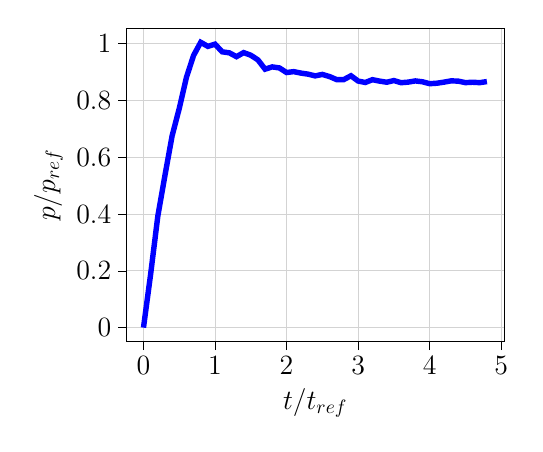
\begin{tikzpicture}[scale=0.7, font=\Large]

\definecolor{lightgray}{RGB}{211,211,211}

\begin{axis}[
tick align=outside,
tick pos=left,
x grid style={lightgray},
xlabel={\(\displaystyle t/t_{ref}\)},
xmajorgrids,
xmin=-0.24, xmax=5.04,
xtick style={color=black},
y grid style={lightgray},
ylabel={\(\displaystyle p/p_{ref}\)},
ymajorgrids,
ymin=-0.0502281761912294, ymax=1.05479170001582,
ytick style={color=black}
]
\addplot [line width=2.8pt, blue]
table {%
0 0
0.1 0.188445766752718
0.2 0.391947508110223
0.3 0.535895204930158
0.4 0.675176372415468
0.5 0.771710290038251
0.6 0.880899367078848
0.7 0.958412412909037
0.8 1.00456352382459
0.9 0.990324948221893
1 0.998054606057314
1.1 0.971102817197564
1.2 0.967556258546069
1.3 0.954084839144053
1.4 0.968359167181806
1.5 0.959116405852193
1.6 0.942617944583139
1.7 0.910026091662552
1.8 0.918049400613525
1.9 0.914348525898006
2 0.898192078875057
2.1 0.901362856789026
2.2 0.896214438996315
2.3 0.892511564645737
2.4 0.886358846124087
2.5 0.891502924804546
2.6 0.884023936770732
2.7 0.873345919605794
2.8 0.873412882862689
2.9 0.886829564180904
3 0.868198311002277
3.1 0.863129333961807
3.2 0.873000347785484
3.3 0.867964509851173
3.4 0.864042793812506
3.5 0.869939165930708
3.6 0.862387111210862
3.7 0.864402846886308
3.8 0.868605632794512
3.9 0.865597652226709
4 0.8589197342603
4.1 0.860522133055493
4.2 0.864358319941601
4.3 0.868875836425173
4.4 0.867843224744737
4.5 0.862641238764823
4.6 0.863963070087864
4.7 0.862565672752955
4.8 0.866328855022948
};
\end{axis}

\end{tikzpicture}

  \hspace{0.5cm}
  % This file was created with tikzplotlib v0.10.1.
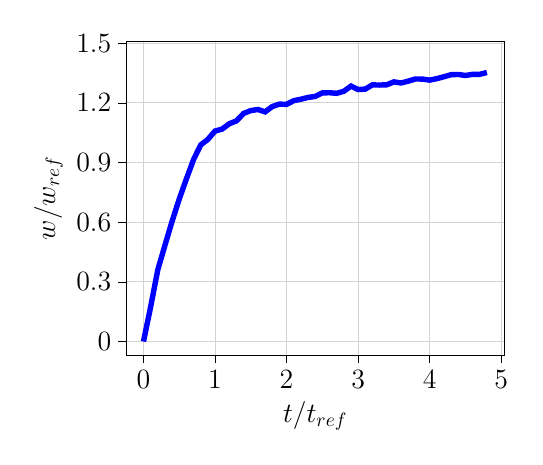
\begin{tikzpicture}[scale=0.7, font=\Large]

\definecolor{lightgray}{RGB}{211,211,211}

\begin{axis}[
tick align=outside,
tick pos=left,
x grid style={lightgray},
xlabel={\(\displaystyle t/t_{ref}\)},
xmajorgrids,
xmin=-0.24, xmax=5.04,
xtick style={color=black},
y grid style={lightgray},
ytick distance=0.3,
ylabel={\(\displaystyle w/w_{ref}\)},
ymajorgrids,
ymin=-0.0676150128188689, ymax=1.51,
ytick style={color=black}
]
\addplot [line width=2.8pt, blue]
table {%
0 0
0.1 0.174099460537345
0.2 0.36037093622801
0.3 0.483736302329922
0.4 0.604657400483929
0.5 0.71627362525909
0.6 0.817741763252065
0.7 0.914673087058184
0.8 0.988043835003288
0.9 1.01615749619579
1 1.05781999647227
1.1 1.06795558571426
1.2 1.09487671410362
1.3 1.10903211791217
1.4 1.14665606861212
1.5 1.16093104459679
1.6 1.16625499737314
1.7 1.15430886393875
1.8 1.18121700420342
1.9 1.19330912726223
2 1.19206895215774
2.1 1.21057291458408
2.2 1.21798236109138
2.3 1.22691783387849
2.4 1.23188777939765
2.5 1.24970648339836
2.6 1.25053556512246
2.7 1.24766343959738
2.8 1.2578584515492
2.9 1.28381515930564
3 1.26659534216305
3.1 1.26894556444263
3.2 1.29005564497642
3.3 1.28918001813621
3.4 1.29050708947248
3.5 1.30520754884353
3.6 1.29951568143079
3.7 1.30872862561227
3.8 1.31974418932991
3.9 1.31922767023963
4 1.31398053120865
4.1 1.32143831069796
4.2 1.33095372857038
4.3 1.34126355648886
4.4 1.34234868328863
4.5 1.33716954069027
4.6 1.34310704227726
4.7 1.34310814299716
4.8 1.35230025637738
};
\end{axis}

\end{tikzpicture}

  \caption{Two quantities of interest for the parallel fracture problem. On the left, the time series of the pressure at the injection point, on the right, the fracture aperture. Both plots show results scaled by reference values, calculated at the onset of propagation.}  
  \label{fig:parallel_fracs_charts}
\end{figure}


\begin{figure}[h]
\begin{subfigure}{.45\textwidth}
  \centering
  \includegraphics[width=\linewidth]{Chapter4/figures/3D/new_t_0.png}
  \caption{}
  \label{fig:parallel_t_0}
\end{subfigure}%
\hspace{1cm}
\begin{subfigure}{.45\textwidth}
  \centering
  \includegraphics[width=\linewidth]{Chapter4/figures/3D/new_t_30.png}
  \caption{}
  \label{fig:parallel_t_1}
\end{subfigure}%

\begin{subfigure}{.45\textwidth}
  \centering
  \includegraphics[width=\linewidth]{Chapter4/figures/3D/new_t_60.png}
  \caption{}
  \label{fig:parallel_t_2}
\end{subfigure}
\hspace{0.85cm}
\begin{subfigure}{.45\textwidth}
  \centering
  \includegraphics[width=\linewidth]{Chapter4/figures/3D/new_t_90.png}
  \caption{}
  \label{fig:parallel_t_3}
\end{subfigure}
  \caption{Snapshots of the simulated propagation. The left side of the figures shows the discrete fracture colored in grayscale according to the aperture and the subdomain colored according the damage value. The right side shows the pressure field in the global domain. (a) Snapshot $t/t_{ref} = 0$; (b) $t/t_{ref} = 1.5$; (c) $t/t_{ref} = 3$; and (d) $t/t_{ref} = 4.5$. } 
  \label{fig:parallel_snapshots}
\end{figure}

\FloatBarrier

\subsection{Merging two circular fractures}

The second problem deals with the case of in-plane fracture merging. In general, fracture merging is one of the most difficult behaviors to simulate with discrete fracture approaches. That is due to the interaction between the stress fields of two fracture fronts, which makes most attempts to extract a stress intensity factor innacurate. In practice, these situation may happen when fracking wells are drilled parallel to each other. 

For problems involving crack merging, the phase-field approach becomes handy, allowing for the computation of crack advances through the solution of PDEs that are independent of the fracture topology.
The multi-resolution approach explore this advantage, keeping a phase-field description around the fracture front and removing the limitations of discrete methods.

Since this problem deals with in-plane merging, getting the discrete fracture planes from the phase-field values is straightforward. However, it is important to mention that this can be a challenge in the case of non-planar merging.

The problem under consideration consists of two parallel fractures, initally of circular shape, embedded in a poroelastic matrix. Both are injected with a viscous fluid and propagate radially, eventually merging. An schematic of the geometry is shown in Figure \ref{fig:merging_schematic}, with the dimensions listed in Table \ref{merging_measures}. As in the previous problem, the far-field boundary conditions are assumed to be homogenous for pressures and displacements. 

As for the discretization, the coarser global mesh consists of a structured grid that is refined near the fracture planes, with an element size of around 0.095m in the width direction and 0.15m in the other directions. The local mesh is 5 times smaller and the regularization length used in the phase-field subproblem is 0.05m. Importantly, the local domain consists of all local elements within a distance of 1m to the fracture front. Initally, they consist of two separate torus, but they eventually merge as the cracks get closer. As for the time-step, it is uniformly set to 0.01s.

The simulated behavior is depicted in Figure \ref{fig:merge_snapshots}, which shows the expected behavior, which the cracks growing perfectly as circles until they approach each other and merge. After the merge, the most concave part of the crack grows and opens up until the pressure drops enough for the propagation to arrest. While there is not reference solution to compare, at least qualitatively, the results make sense. As for the previous problem, the times series for the aperture and pressure in the injection point are shown in Figure \ref{fig:merging_charts}. The reference values used to make these charts nondimensional are given in Table \ref{merging_refs}.

\begin{table}[ht]
  \centering
  \caption{Domain dimensions}
  \begin{tabular}[t]{lccccccc}
  \hline
  &$d_1$&$d_2$&$d_3$&$L_x$&$L_y$&$L_z$&$r$\\  
  \hline
  Value (m) & 6.5 & 7.0 & 6.5 & 8.0 & 20.0 & 5.0 & 1.5\\
  \hline
  \end{tabular}
  \label{merging_measures}
\end{table}%

\begin{table}[ht]
  \centering
  \caption{Reference values used in the time series plots.}
  \begin{tabular}[t]{lcc}
  \hline
  &Value &Unit \\
  \hline
  $p_{ref}$&520&MPa\\
  $w_{ref}$&7.0$\times 10^{-4}$&m\\
  $t_{ref}$&10&$\text{s}$\\
  \hline
  \end{tabular}
  \label{merging_refs}
\end{table}%

\begin{figure}[ht]
  \centering
  \begin{tikzpicture}
      \node {\pgfimage[interpolate=false,width=.8\textwidth]{Chapter4/figures/merging/merging_schematic.png}};
      \draw (0.0\textwidth,0.07\textwidth) node {\large$r$};
      \draw (0.37\textwidth,0.12\textwidth) node {\large$L_x$};
      \draw (0.04\textwidth,-0.25\textwidth) node {\large$L_y$};
      \draw (0.42\textwidth,-0.07\textwidth) node {\large$L_z$};
      \draw (-0.25\textwidth,0.25\textwidth) node {\large$d_1$};
      \draw (-0.03\textwidth,0.25\textwidth) node {\large$d_2$};
      \draw (0.2\textwidth,0.25\textwidth) node {\large$d_3$};
  \end{tikzpicture}
  \caption{Schematic of the geometry for the merging problem.}
  \label{fig:merging_schematic}
\end{figure}


\begin{figure}[h]
\noindent% This file was created with tikzplotlib v0.10.1.
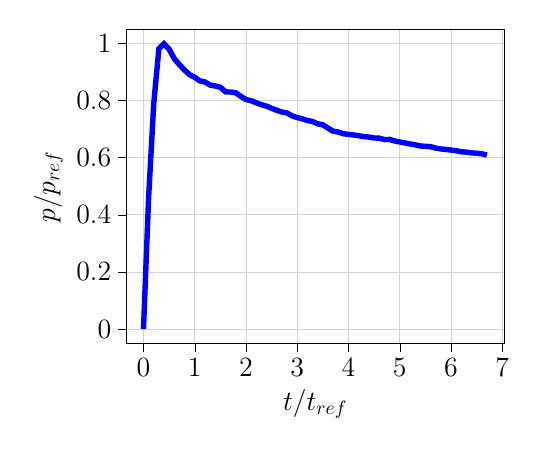
\begin{tikzpicture}[scale=0.7, font=\Large]

\definecolor{lightgray}{RGB}{211,211,211}

\begin{axis}[
tick align=outside,
tick pos=left,
x grid style={lightgray},
xlabel={\(\displaystyle t/t_{ref}\)},
xmajorgrids,
xmin=-0.335, xmax=7.035,
xtick style={color=black},
y grid style={lightgray},
ylabel={\(\displaystyle p/p_{ref}\)},
ymajorgrids,
ymin=-0.0498825329280283, ymax=1.0475331914886,
ytick style={color=black}
]
\addplot [line width=2.8pt, blue]
table {%
0 0
0.1 0.45951217560765
0.2 0.788592266536983
0.3 0.979658043857808
0.4 0.997650658560567
0.5 0.978785067303964
0.6 0.945971757956235
0.7 0.924877167218727
0.8 0.905966129538245
0.9 0.889602759640749
1 0.880357526928354
1.1 0.867671216379265
1.2 0.864233448832077
1.3 0.853114312789821
1.4 0.850108135287821
1.5 0.845620481022948
1.6 0.829505321551291
1.7 0.82892647153026
1.8 0.826514080553166
1.9 0.813655142687903
2 0.802768783688767
2.1 0.798543387344519
2.2 0.791408224631453
2.3 0.784592950157044
2.4 0.779669735090534
2.5 0.771982941261582
2.6 0.764935123584626
2.7 0.759180136109881
2.8 0.755819802453577
2.9 0.745394700232725
3 0.739759343297616
3.1 0.73509236716247
3.2 0.729345702728615
3.3 0.725778734141958
3.4 0.717687645906032
3.5 0.714371573361759
3.6 0.702688940886406
3.7 0.692071117257683
3.8 0.689075788412169
3.9 0.683018346545578
4 0.680940241480926
4.1 0.678761582675207
4.2 0.676155909908243
4.3 0.67303862482668
4.4 0.67141982291266
4.5 0.668213339195578
4.6 0.667744559568312
4.7 0.662721346127251
4.8 0.663129635213632
4.9 0.657892335911165
5 0.654296951897791
5.1 0.650863757765831
5.2 0.647428666367983
5.3 0.644241597549297
5.4 0.640318013987773
5.5 0.638947287170507
5.6 0.638052591816986
5.7 0.632877744620429
5.8 0.629874714646489
5.9 0.62812562862508
6 0.625989632848015
6.1 0.623727478456361
6.2 0.61994558051626
6.3 0.618837276024664
6.4 0.616144894474259
6.5 0.614945973289227
6.6 0.612979236533847
6.7 0.60828213805131
};
\end{axis}

\end{tikzpicture}
\hspace{0.5cm}
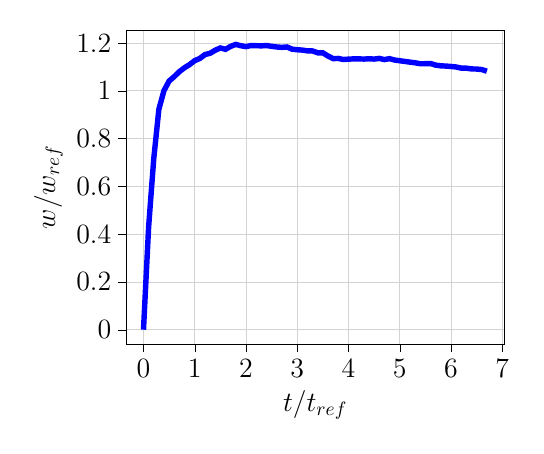
\begin{tikzpicture}[scale=0.7, font=\Large]

\definecolor{lightgray}{RGB}{211,211,211}

\begin{axis}[
tick align=outside,
tick pos=left,
x grid style={lightgray},
xlabel={\(\displaystyle t/t_{ref}\)},
xmajorgrids,
xmin=-0.335, xmax=7.035,
xtick style={color=black},
y grid style={lightgray},
ylabel={\(\displaystyle w/w_{ref}\)},
ymajorgrids,
ymin=-0.0597293287257296, ymax=1.25431590324032,
ytick style={color=black}
]
\addplot [line width=2.8pt, blue]
table {%
0 0
0.1 0.42960065054532
0.2 0.715136605775466
0.3 0.922750840112107
0.4 1.0013207791429
0.5 1.0411598779676
0.6 1.05982581607324
0.7 1.08050584575762
0.8 1.09671277193648
0.9 1.11032136558952
1 1.12663033076329
1.1 1.13590704337549
1.2 1.15199446917512
1.3 1.15745805434228
1.4 1.17029484955157
1.5 1.1797256365628
1.6 1.17401971466754
1.7 1.18622756700584
1.8 1.19458657451459
1.9 1.18892597827636
2 1.18545966357443
2.1 1.18983889045998
2.2 1.18920351864721
2.3 1.18850491342986
2.4 1.18987192915262
2.5 1.18655089416824
2.6 1.18376216613162
2.7 1.18232996709817
2.8 1.18384178574721
2.9 1.1745917982695
3 1.17218634899917
3.1 1.17081354140302
3.2 1.1674404732521
3.3 1.16714196039589
3.4 1.15942128056545
3.5 1.15905443325056
3.6 1.14598602032622
3.7 1.13512321674529
3.8 1.13577811166775
3.9 1.13137169873407
4 1.13287911123356
4.1 1.13401684532316
4.2 1.13401065495831
4.3 1.13319092621984
4.4 1.13446327534522
4.5 1.13314924992658
4.6 1.13590775886393
4.7 1.13102049244932
4.8 1.13486709640336
4.9 1.12912798009531
5 1.12617496099899
5.1 1.12326496239068
5.2 1.1202902089975
5.3 1.11761318780537
5.4 1.11361031173121
5.5 1.11379000169957
5.6 1.11459022130972
5.7 1.10788856842442
5.8 1.1048189314348
5.9 1.10389204151723
6 1.10216294677504
6.1 1.10006683973921
6.2 1.09525678021556
6.3 1.09503757716002
6.4 1.09193800888068
6.5 1.09139905221393
6.6 1.08928999986265
6.7 1.08233446321413
};
\end{axis}

\end{tikzpicture}
\caption{Two quantities of interest for the merging fracture problem. On the left, the time series of the pressure at the injection point, on the right, the fracture aperture. Both plots show results scaled by reference values, calculated at the onset of propagation.}  
\label{fig:merging_charts}
\end{figure}


\begin{figure}[h]
\begin{subfigure}{.45\textwidth}
  \centering
  \includegraphics[width=\linewidth]{Chapter4/figures/merging/merging_t_1.png}
  \caption{}
  \label{fig:merge_t_0}
\end{subfigure}%
\hspace{1cm}
\begin{subfigure}{.45\textwidth}
  \centering
  \includegraphics[width=\linewidth]{Chapter4/figures/merging/merging_t_14.png}
  \caption{}
  \label{fig:merge_t_1}
\end{subfigure}%

\begin{subfigure}{.45\textwidth}
  \centering
  \includegraphics[width=\linewidth]{Chapter4/figures/merging/merging_t_27.png}
  \caption{}
  \label{fig:merge_t_2}
\end{subfigure}
\hspace{0.85cm}
\begin{subfigure}{.45\textwidth}
  \centering
  \includegraphics[width=\linewidth]{Chapter4/figures/merging/merging_t_35.png}
  \caption{}
  \label{fig:merge_t_3}
\end{subfigure}

\begin{subfigure}{.45\textwidth}
  \centering
  \includegraphics[width=\linewidth]{Chapter4/figures/merging/merging_t_42.png}
  \caption{}
  \label{fig:merge_t_4}
\end{subfigure}
\hspace{0.85cm}
\begin{subfigure}{.45\textwidth}
  \centering
  \includegraphics[width=\linewidth]{Chapter4/figures/merging/merging_t_67.png}
  \caption{}
  \label{fig:merge_t_5}
\end{subfigure}
  \caption{Snapshots of the simulated propagation. The discrete fracture is colored in grayscale according to the aperture and the subdomain colored according the damage value. (a) Snapshot $t/t_{ref} = 0$; (b) $t/t_{ref} = 1.3$; (c) $t/t_{ref} = 2.6$; (d) $t/t_{ref} = 3.9$; (e) $t/t_{ref} = 5.2$; and (f) $t/t_{ref} = 6.5$. } 
  \label{fig:merge_snapshots}  
\end{figure}

\FloatBarrier




\section{Extension to non-planar fractures}
\label{section: Chapter4/nonplanar}

While in several practical cases, such as in layered formation, the assumption of planar fractures is recommended \cite{mcclure2020planar}, in many others, a general treatment that allows for non-planar growth in needed. However, in the context of the multi-resolution approach presented herein, this extension requires additional challenges to be addressed. In the last Section of this work, these challenges are discussed and a skeleton of a possible modified algorithm is described. A simplified nonplanar fracture problem in 2D is then used to test it. Although the result is favorable, the extension of this algorithm to full 3D problems requires additional modifications whose robustness is unclear. 

\subsection{Overview of a propagation algorithm for non-planar fractures}\label{basicNonplanarAlgo}

In Section \ref{section: Chapter4/algo}, the algorithm \ref{fig:MR_planar_algo} showed how to use the multi-resolution method to treat planar fractures in 3D. To extend it to non-planar cases, at a minimum, the following parts must be modified. 

\begin{itemize}
    \item First, the algorithm for tracking the damage in the front elements described in subsection \ref{frontTrackingAlgo} must be revisited, considering that the damage field is not planar. That definitely breaks the hypothesis of the damage volume criterion and also introduces pathological cases that make the applicability of the topological criterion more difficult.
    
    \item The update of the geometry becomes more complex for the same reason. Given a nonplanar damage field in an element, how to insert a planar\footnote{While it is possible to develop embedded methods that allow for curved cuts inside elements, those are rarely used in practice due to the complex integration techiniques needed. Because of that, in the current work, while strong assumptions on the embedded scheme are avoided, the focus is on first-order (i.e planar cuts) methods.} cut in the mesh that represents it well?
    
    \item Finally, while for planar cuts the continuity of the fracture surface is always guaranteed, in nonplanar case, local (element-wise) approximations of the damage field with discrete cuts may lead to gaps in the fracture surface, such as the ones shown in Figure \ref{fig:gaps}.
\end{itemize}

To address the first bullet point, one can start with the topological criterion proposed in \ref{frontTrackingAlgo}, where the number of edges and faces with damage above a threshold is used. In general, if the damage band is small compared to the global element size, there is likely no ambiguity in the identification of cutting points. However, if the regularization length or the mesh size in the local problem are not very small, some difficulties may arise. For example, a wide damage band approaching the element diagonally may cut two adjacent edges as shown in Figure \ref{fig:pathological_case}. This leads to a configuration where the number of cut edges and faces is large albeit the actual global element is not yet fractured. 

\begin{figure}
    \centering
    \includegraphics[width=\linewidth]{Chapter4/figures/nonplanar/pathology.png}
    \caption{This figure shows a pathological case for the topological criterion proposed in \ref{frontTrackingAlgo}. The element on the right is only partially damaged, however, the counts of cut edges and faces are higher than the ones for the element on the left, which is indeed fully cut.}
    \label{fig:pathological_case}
\end{figure}%

Overcoming this limitation likely requires the use of information about the damage in neighboring elements. One approach, used in the example problem shown next, keeps the topological criterion the same, but introduces a check on the cutting angle that is obtained after an element is cut. This check consists of comparing the normal to the new cut with the neighboring fractured elements. If the normals are too different (i.e $\textbf{n}\cdot\textbf{n}_{neighbor} << 1$), then, this newly inserted cut is assumed to be due to a pathological case and then removed. The respective element is only considered for cutting again when the number of damaged faces increases. This check will be refered to as ``the angle check".

This heuristic relies on the assumption that fractures do not kink strongly over element boundaries, which is only true if the fracture curves have a large radius of curvature compared to the global element size. 

Now, in terms of the second bullet point, regarding the extraction of the cutting plane from a damage field, an optimization algorithm such as \cite{geelen2018optimization} can be employed. In a nutshell, this method searchs over the space of planes embedded in an element and constructs an idealized damage profile around this plane, using the optimal profile\footnote{This is the profile for an AT-1 phase-field formulation.} given by $d(x) = (1-\text{dist}(x)/2\ell)^2$, where $\text{dist}(x)$ denotes the distance from $x$ to the plane. These idealized profiles are then compared to the actual damage field and the one which is closest in the $L_2$-sense is chosen to be the cutting plane for that damage field.

One must be careful when integrating this optimization approach with the angle check described above. That heuristic works under the assumption that an attempted cut on an element which is not yet fractured will lead to a cutting plane that does not conform well to its neighbors. If an optimization approach is employed, that might not always be true. For example, in the case shown in Figure \ref{fig:pathological_case}, the optimization approach can find the cutting plane induced by the partial fracture which will conform well to the existing cuts, even though the element is only partially cut.

So, in order to use the angle check, instead of applying the optimization method and then comparing the calculated plane with its neighbors, the idea of a coarser ``pre-cut'' is used. The idea of these pre-cuts is to rely only on the relative position of the cut identified in the element edges and faces by the topological criterion. This is done to ensure that, if one is dealing with a pathological case for the topological criterion, the pre-cut will indicate that and fail the angle check. In a 2D scenario, these pre-cuts can be obtained for example, by connecting the midpoints of the fractured faces. In 3D, the mapping becomes more complex. Figure \ref{fig:pre_cuts} shows the four basic ways that a plane can intersect a brick element, rotations and reflections also need to be included. The pre-cut to be chosen for an element in 3D can then be obtained by evaluating which of these best approximate the set of damaged faces computed by the topological criterion for that element (based on its damage field in the local scale). 

\begin{figure}[h]
    \centering
    \includegraphics[width=0.8\linewidth]{Chapter4/figures/nonplanar/pre_cuts.png}
    \caption{Basic shapes for a planar cut in a brick element.}
    \label{fig:pre_cuts}
\end{figure}

Even with these modifications, the third and last bullet point, that concerns the continuity of the fracture surface must be addressed. For general embedded fracture approaches, continuity of the fracture surface is a necessary feature for the construction of the approximation space for the displacement field. This imposes serious complications to any type of algorithm that tries to construct surface increments on an element to element basis such as the one used here. However, the EFEM/EDFM approach used in this work and first proposed in \cite{cusini2021simulation} does offer a possible way to handle this issue. Unfortunately, that does break the generality of the multi-resolution approach with respect to the discretization techinique used in the global domain. 

By construction, the EFEM method does not assume continuity of the displacement field across element boundaries. In fact, the enrichment employed to represent the displacement jump does not interact with the neighboring elements and the final aperture might indeed be discontinuous. Still, the method does converge to the continuous solution in space. Figure \ref{fig:efem_apertures}, from \cite{cusini2021simulation} shows a typical aperture field computed with EFEM. This flexibility allows one to work with a fracture surface that has gaps in its geometry and still compute an accurate aperture field. 

\begin{figure}[h]
    \centering
    \includegraphics[width=0.5\linewidth]{Chapter4/figures/nonplanar/efem_aperture.png}
    \caption{This figure shows how the aperture field computed with EFEM approaches an analytical solution as the mesh is refined. Note that the aperture field is discontinuity across element boundaries. Courtesy from \cite{cusini2021simulation}}
    \label{fig:efem_apertures}
\end{figure}

On the other hand, for the computation of the flow problem, continuity is still required to calculate fluxes from a fracture cell to its neighbors. In fact, two compute the flux between two embedded cells, their common edge is used. That is, if one obtains a discontinuous fracture surface, there will be neighboring cells that do not share an edge and therefore, the flux between them will be zero.

Luckly, this issue can be circuvented by noting that the damage intersection on any edge is the same for all elements that contain that edge. Therefore, instead of computing the fluxes directly from the common edge of neighboring fracture cells, one can store the intersections of the damage field with the global element edges and use them to build segments in between two neighboring cells. These segments can them be used to compute the fluxes, ensuring that even neighboring cells that happen to be on a surface discontinuity still get a unique, meaningful flux. Figure \ref{fig:flux_calculations} shows two neighboring fracture elements that form a gap. In this case, the damage intersections D1 and D2 should be use to define the common edge that enters the flux calculation.

\begin{figure}[h]
    \centering
    \includegraphics[width=0.6\linewidth]{Chapter4/figures/nonplanar/nonplanar_flux.png}
    \caption{Flux in discontinuous fracture surfaces. D1 and D2 are the intersections of the damage field with the edges and serve to define a line segment that can be used to calculate the flux between the two fracture elements.}
    \label{fig:flux_calculations}
\end{figure}

Combining all the workaround described in this Section, we can obtain an algorithm that extends algorithm \ref{fig:MR_planar_algo} to allow for the treatment of non-planar fractures with a multi-resolution scheme. These modification are displayed as an algorithm in Figure \ref{fig:nonplanar_algo}.

While this algorithm theoretically answers most of the challenges discussed in this Section, a full implementation for general 3D problems is not yet completed. Currently, only the first modification to the algorithm, which concerns the topological criterion and its enhancement with the angle check and pre-cuts is implemented and tested. The optimization scheme and the flux computations based on the damage interesections in the edges are left for future investigations. 

\begin{figure}[h]
    \centering
    \includegraphics[width=\linewidth]{Chapter4/figures/nonplanar/nonplanar_algo.png}
    \caption{Enhancements to \ref{fig:MR_planar_algo} to allow for non-planar fracture propagation.}
    \label{fig:nonplanar_algo}
\end{figure}


In the next section, this simplification of the algorithm described above is applied to a 2.5D problem where the crack path is curved. It serves to check the efficacy of the proposed changes in the process of identifying the crack path. The fluid flow and poroelastic effects are turned off for simplicity.

\subsection{Example problem}

This subsection presents a small 2D problem used to test some features of the algorithm presented in \ref{basicNonplanarAlgo}. The problem consists of an edge crack in a square plate, which is pulled in the top edge by an inclined displacement $\Delta u$, at an angle of 45deg, as shown in Figure \ref{fig:nonplanar_schematic}. The bottom surface is held fixed while the sides are left with a zero traction boundary condition. The material properties and geometric parameters are given in Table \ref{material properties nonplanar}. All the fluid effects are removed, as the focus is only on the algorithm to track the fracture and insert the discrete cuts. The subdomain is set to be the entire domain, which simplifies the transfer of boundary conditions from the global to local problem. 

\begin{table}[h]
    \centering
    \caption{Material properties for non-planar fracture problem.}
    \begin{tabular}[t]{lcc}
    \hline
    &Value &Unit \\
    \hline
    Young's modulus ($E$)&16.0&GPa\\
    Poisson's ratio ($\nu$)&0.18&--\\
    Critical energy release rate ($G_c$)&2.5&$\text{N/m}$\\
    Regularization length ($\ell$)&0.04&$\text{m}$\\
    Applied displacement ($\Delta u$)&$2.0\times 10^{-5}$&$\text{m}$\\
    Initial crack length (a)&2.5&$\text{m}$\\
    Plate size (L)&5.0&$\text{m}$\\
    \hline
    \end{tabular}
    \label{material properties nonplanar}
\end{table}%

In terms of discretization, the coarser global mesh uniformly splits the domain in 21x21 elements, with the finer grid being 11 times smaller. That leads to a subdomain element whose size is 2 times smaller than the phase-field regularization length. The load increment used was $2.0\times 10^{-7}$ m. 

A very similar problem was studied in \cite{giovanardi2017hybrid}. Despite the differences in material properties, it serves as a reference solution for the crack path, which is the main quantity of interest for this analysis. So, their results are shown in Figure \ref{fig:reference result}. Despite the simplification in defining the cut direction, the discrete fracture is still capable of tracking the damage band quite well, as shown in Figure \ref{fig:crack_path}, displaying a great agreement with the reference solution. Interestingly, this problem involves multiple cases of the damage band approaching the diagonal of an element, which constitutes a pathological case, described previously. This shows that the correction based on the neighboring cutting angles is indeed useful and necessary in this type of approach.

A relative straightforward improvement can be done with the introduction of an optimization method, as discusssed in \ref{basicNonplanarAlgo} to produce cuts that better align with the damage band locally. However, the use of "crude" approximations (pre-cuts) is still important to test the angle criteria and prevent lighly damaged elements from being wrongly cut due to a pathological case, such as the one shown in Figure \ref{fig:pathological_case}.

One the downside, this example doesn't explore a lot of the difficulties that arise in general three-dimensional problems. 
First, creating a map between the damaged faces and the pre-cuts shown in Figure \ref{fig:pre_cuts} becomes much more difficult in 3D. In addition to that, the angle criteria may work well in cracks that evolve progressively as the one in this example, however, it may get into a ``locking" situation if two cracks are merging at an angle. This is, different neighbors may impose constraints in the cutting angle of an element that may be impossible to satisfy simultaneously. 

Overcoming these challegens likely requires a more severe reformulation of the algorithm used for planar fractures. One promising approach is to employ a global method of surface reconstruction after the solution of the phase-field problem. This is a research topic on its own, with important contributions developed in recent years, such as \cite{yang2021explicit, zeng2022tracking, xu2023reconstruct}. In the context of hybrid phase-field methods, the authors of \cite{eldahshan2021cipfar} used a global surface reconstruction to improve the simulation of ductile fracture. They used the gradient of the damage to guide the identification of a discrete fracture surface embedded in a triangular mesh. While the robustness of their reconstruction in the presence of crack merging and branching is still unclear, it certainly points to a promising direction that can be explored in the context of the multi-resolution approach for hydraulic fracture.

\begin{figure}[ht]
    \centering
    \begin{tikzpicture}
        \node {\pgfimage[interpolate=false,width=.4\textwidth]{/home/andre/projects/Dissertation/dissertation/Chapter4/figures/nonplanar/nonplanar_schematic.png}};
        \draw (-0.1\textwidth,0.04\textwidth) node {\large$a$};
        \draw (0.22\textwidth,0.0\textwidth) node {\large$L$};
        \draw (0.02\textwidth,0.23\textwidth) node {\large$\Delta\textbf{u}$};
    \end{tikzpicture}
    \caption{Schematic of the edge crack problem. The load of the top surface is inclined 45deg, which leads to a curved fracture path.}
    \label{fig:nonplanar_schematic}
\end{figure}

\begin{figure}[h]
    % \centering
    \begin{subfigure}{.45\textwidth}
      \centering
      \includegraphics[width=0.765\linewidth]{Chapter4/figures/nonplanar/curved_crack_result_bianca.png}
      \caption{Crack path - Giovanardi et al. \cite{giovanardi2017hybrid}.}
      \label{fig:reference result}
    \end{subfigure}%
    \begin{subfigure}{.54\textwidth}
      \centering
      \includegraphics[width=0.83\linewidth]{Chapter4/figures/nonplanar/nonplanar_example.png}
      \caption{Crack path - current work}
      \label{fig:crack_path}
    \end{subfigure}%
      \caption{Comparision of the crack paths obtained for the edge crack problem. Despite the roughness of the crack path in (b), the overall path compares very well to the reference result.} 
      \label{fig:nonplanar_example}
\end{figure}

% \section{Numerical examples}
\label{section: Chapter4/examples}

In this Section, a two example problems computed with the aforementioned method are presented. These examples illustrate the main capabilities of the approach, but also serve to demonstrate some of the limitations. They all consist of hydrulic fracture propagation in a poroelastic medium involving different fracture configurations that are relevant to practical fracking applications. The main goal is to ensure that the proposed algorithm supports these two representative scenarios and that it can be used to simulate real world fracking treatments whenever the assumption of planar growth is adequate. 

Importantly, a true verification procedure is not performed here. For example, mesh convergence studies and comparisons with well-known solutions are yet to be performed for these 3D problems as we did in Chapter \ref{section: Chapter3}. These require a few enhancements in the solver technology that are currently under development. First, due to the high discrepancy between the scales of degrees of freedom (matrix displacements, fracture apertures and pressures), general purpose linear solvers struggle to converge when the meshes are refined past a certain point. Because of that, special preconditioners that take into account the block structure of the system are being developed. Second, analytical solutions for poroelastic problems are scarce, so, a common verification procedure consists in solving them with vanishing small permeability coefficients to verify convergence towards the impermeable case, which does have a closed-form solution. However, as the permeability decreses, the poromechanics problem starts to display spurious pressure oscillations unless LBB-stable elements \cite{arnold1984stable} or a stabilized formulations, such as \cite{white2008stabilized} are used. These enhancements in the solver infrastructure are left for future work.

For the two problems in this Section, the material properties used are listed in Table \ref{material properties ch4}. The fluid injection rate $Q$ is set to $2.0 m^3/s$ (on each injection point).

\begin{table}[h]
  \centering
  \caption{Material properties for planar fracture problems.}
  \begin{tabular}[t]{lcc}
  \hline
  &Value &Unit \\
  \hline
  Young's modulus ($E$)&16.0&GPa\\
  Poisson's ratio ($\nu$)&0.18&--\\
  Fluid viscosity ($\mu$)&1.0$\times10^{-12}$&$\text{GPa . s}$\\
  Fluid bulk modulus ($K_f$)&1.0$\times10^{10}$&$\text{GPa}$\\
  Critical energy release rate ($G_c$)&2.5&$\text{N/m}$\\
  Biot coefficient ($\alpha$)&1.0&$\text{ - }$\\
  Rock permeability ($\kappa_0$)&1.0$\times 10^{-13}$&$\text{m}^2$\\
  Initial porosity ($\phi_0$)&0.2&$\text{-}$\\
  \hline
  \end{tabular}
  \label{material properties ch4}
\end{table}%

\subsection{Two parallel circular fractures under fluid injection}

In the first problem, a pair of parallel penny-shaped fractures is stimulated with the injection of a viscous fluid. This configuration is representative of a very common scenario in real-world fracking treatments where, in general, there are multiple clusters with several parallel fractures in each. Their simultaneous stimulation can lead to all fractures growing simultaneously or to situations in which only a few show substantial propagation while the others arrest early in the process. These scenarios can lead to very different well behaviors.   

Depending on the distance between the fractures, there may also be non-planar growth, with fractures propagating away from each other, forming a cup shaped geometry. This is a consequence of the interaction between the stress fields in the vicinity of the multiple fractures fronts. This interaction is often called stress shadow effect. In this numerical example shown here, the initial fractures are placed far from each other to prevent this non-planar behavior. The far-field boundary conditions are assumed to be homogenous for pressures and displacements. Figure \ref{fig:parallel_schematic} illustrates the geometry. The dimensions are described in Table \ref{parallel_measures}.

As for the discretization, the coarser global mesh consists of a structured grid that is refined near the fracture planes, with an element size of around 0.075m in the width direction and 0.15m in the other directions. The local mesh is 5 times smaller and the regularization length used in the phase-field subproblem is 0.05m. Importantly, the local domain consists of all local elements within a distance of 1m to the fracture front. Since the fractures are penny shaped, this local domain will have the shape of a torus. As for the time-step, it is uniformly set to 0.01s.

Due to the uniform boundary conditions and homogenous material properties, the fractures are expected to grow radially, preserving their circular shape. This feature is confirmed in the simulated results shown in Figure \ref{fig:parallel_snapshots}. In these snapshots, the right-side of the domain shows the pressure field computed in the global domain whereas the left side shows the discrete crack geometry, colored in gray scale indicating the aperture field. This figure also shows the subdomain around the crack front, colored by the damage field.

The aperture and pressure at the injection sources are important quantities of interest in this type of problem and their simulated time series are shown in Figure \ref{fig:parallel_fracs_charts}. Due to the symmetry, both fractures have the same pressure and aperture results. The reference values used to make the curves nondimensional are listed in Table \ref{parallel_refs}.

\begin{table}[ht]
  \centering
  \caption{Domain dimensions}
  \begin{tabular}[t]{lccccccc}
  \hline
  &$d_1$&$d_2$&$d_3$&$L_x$&$L_y$&$L_z$&$r$\\  
  \hline
  Value (m) & 4.0 & 8.0 & 4.0 & 16.0 & 5.0 & 5.0 & 1.3\\
  \hline
  \end{tabular}
  \label{parallel_measures}
\end{table}%

\begin{table}[ht]
  \centering
  \caption{Reference values used in the time series plots.}
  \begin{tabular}[t]{lcc}
  \hline
  &Value &Unit \\
  \hline
  $p_{ref}$&$320$&MPa\\
  $w_{ref}$&$5.0\times10^{-4}$&m\\
  $t_{ref}$&$10$&$\text{s}$\\
  \hline
  \end{tabular}
  \label{parallel_refs}
\end{table}%

\begin{figure}[ht]
  \centering
  \begin{tikzpicture}
      \node {\pgfimage[interpolate=false,width=0.8\textwidth]{Chapter4/figures/3D/parallel_schematic.png}};
      \draw (-0.11\textwidth,0.185\textwidth) node {\large$r$};
      \draw (0.3\textwidth,0.12\textwidth) node {\large$L_x$};
      \draw (0.1\textwidth,-0.31\textwidth) node {\large$L_y$};
      \draw (0.42\textwidth,-0.15\textwidth) node {\large$L_z$};
      \draw (-0.05\textwidth,0.3\textwidth) node {\large$d_1$};
      \draw (0.02\textwidth,0.23\textwidth) node {\large$d_2$};
      \draw (0.09\textwidth,0.15\textwidth) node {\large$d_3$};
  \end{tikzpicture}
  \caption{Schematic of the problem geometry.}
  \label{fig:parallel_schematic}
\end{figure}


\begin{figure}[h]
  \noindent% This file was created with tikzplotlib v0.10.1.
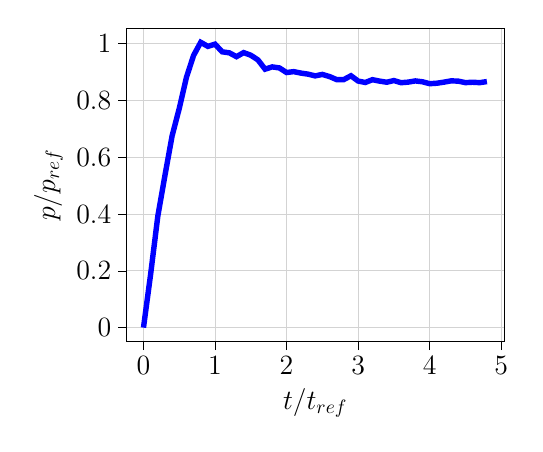
\begin{tikzpicture}[scale=0.7, font=\Large]

\definecolor{lightgray}{RGB}{211,211,211}

\begin{axis}[
tick align=outside,
tick pos=left,
x grid style={lightgray},
xlabel={\(\displaystyle t/t_{ref}\)},
xmajorgrids,
xmin=-0.24, xmax=5.04,
xtick style={color=black},
y grid style={lightgray},
ylabel={\(\displaystyle p/p_{ref}\)},
ymajorgrids,
ymin=-0.0502281761912294, ymax=1.05479170001582,
ytick style={color=black}
]
\addplot [line width=2.8pt, blue]
table {%
0 0
0.1 0.188445766752718
0.2 0.391947508110223
0.3 0.535895204930158
0.4 0.675176372415468
0.5 0.771710290038251
0.6 0.880899367078848
0.7 0.958412412909037
0.8 1.00456352382459
0.9 0.990324948221893
1 0.998054606057314
1.1 0.971102817197564
1.2 0.967556258546069
1.3 0.954084839144053
1.4 0.968359167181806
1.5 0.959116405852193
1.6 0.942617944583139
1.7 0.910026091662552
1.8 0.918049400613525
1.9 0.914348525898006
2 0.898192078875057
2.1 0.901362856789026
2.2 0.896214438996315
2.3 0.892511564645737
2.4 0.886358846124087
2.5 0.891502924804546
2.6 0.884023936770732
2.7 0.873345919605794
2.8 0.873412882862689
2.9 0.886829564180904
3 0.868198311002277
3.1 0.863129333961807
3.2 0.873000347785484
3.3 0.867964509851173
3.4 0.864042793812506
3.5 0.869939165930708
3.6 0.862387111210862
3.7 0.864402846886308
3.8 0.868605632794512
3.9 0.865597652226709
4 0.8589197342603
4.1 0.860522133055493
4.2 0.864358319941601
4.3 0.868875836425173
4.4 0.867843224744737
4.5 0.862641238764823
4.6 0.863963070087864
4.7 0.862565672752955
4.8 0.866328855022948
};
\end{axis}

\end{tikzpicture}

  \hspace{0.5cm}
  % This file was created with tikzplotlib v0.10.1.
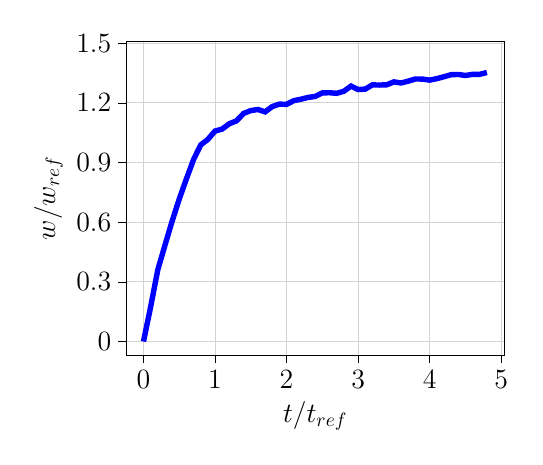
\begin{tikzpicture}[scale=0.7, font=\Large]

\definecolor{lightgray}{RGB}{211,211,211}

\begin{axis}[
tick align=outside,
tick pos=left,
x grid style={lightgray},
xlabel={\(\displaystyle t/t_{ref}\)},
xmajorgrids,
xmin=-0.24, xmax=5.04,
xtick style={color=black},
y grid style={lightgray},
ytick distance=0.3,
ylabel={\(\displaystyle w/w_{ref}\)},
ymajorgrids,
ymin=-0.0676150128188689, ymax=1.51,
ytick style={color=black}
]
\addplot [line width=2.8pt, blue]
table {%
0 0
0.1 0.174099460537345
0.2 0.36037093622801
0.3 0.483736302329922
0.4 0.604657400483929
0.5 0.71627362525909
0.6 0.817741763252065
0.7 0.914673087058184
0.8 0.988043835003288
0.9 1.01615749619579
1 1.05781999647227
1.1 1.06795558571426
1.2 1.09487671410362
1.3 1.10903211791217
1.4 1.14665606861212
1.5 1.16093104459679
1.6 1.16625499737314
1.7 1.15430886393875
1.8 1.18121700420342
1.9 1.19330912726223
2 1.19206895215774
2.1 1.21057291458408
2.2 1.21798236109138
2.3 1.22691783387849
2.4 1.23188777939765
2.5 1.24970648339836
2.6 1.25053556512246
2.7 1.24766343959738
2.8 1.2578584515492
2.9 1.28381515930564
3 1.26659534216305
3.1 1.26894556444263
3.2 1.29005564497642
3.3 1.28918001813621
3.4 1.29050708947248
3.5 1.30520754884353
3.6 1.29951568143079
3.7 1.30872862561227
3.8 1.31974418932991
3.9 1.31922767023963
4 1.31398053120865
4.1 1.32143831069796
4.2 1.33095372857038
4.3 1.34126355648886
4.4 1.34234868328863
4.5 1.33716954069027
4.6 1.34310704227726
4.7 1.34310814299716
4.8 1.35230025637738
};
\end{axis}

\end{tikzpicture}

  \caption{Two quantities of interest for the parallel fracture problem. On the left, the time series of the pressure at the injection point, on the right, the fracture aperture. Both plots show results scaled by reference values, calculated at the onset of propagation.}  
  \label{fig:parallel_fracs_charts}
\end{figure}


\begin{figure}[h]
\begin{subfigure}{.45\textwidth}
  \centering
  \includegraphics[width=\linewidth]{Chapter4/figures/3D/new_t_0.png}
  \caption{}
  \label{fig:parallel_t_0}
\end{subfigure}%
\hspace{1cm}
\begin{subfigure}{.45\textwidth}
  \centering
  \includegraphics[width=\linewidth]{Chapter4/figures/3D/new_t_30.png}
  \caption{}
  \label{fig:parallel_t_1}
\end{subfigure}%

\begin{subfigure}{.45\textwidth}
  \centering
  \includegraphics[width=\linewidth]{Chapter4/figures/3D/new_t_60.png}
  \caption{}
  \label{fig:parallel_t_2}
\end{subfigure}
\hspace{0.85cm}
\begin{subfigure}{.45\textwidth}
  \centering
  \includegraphics[width=\linewidth]{Chapter4/figures/3D/new_t_90.png}
  \caption{}
  \label{fig:parallel_t_3}
\end{subfigure}
  \caption{Snapshots of the simulated propagation. The left side of the figures shows the discrete fracture colored in grayscale according to the aperture and the subdomain colored according the damage value. The right side shows the pressure field in the global domain. (a) Snapshot $t/t_{ref} = 0$; (b) $t/t_{ref} = 1.5$; (c) $t/t_{ref} = 3$; and (d) $t/t_{ref} = 4.5$. } 
  \label{fig:parallel_snapshots}
\end{figure}

\FloatBarrier

\subsection{Merging two circular fractures}

The second problem deals with the case of in-plane fracture merging. In general, fracture merging is one of the most difficult behaviors to simulate with discrete fracture approaches. That is due to the interaction between the stress fields of two fracture fronts, which makes most attempts to extract a stress intensity factor innacurate. In practice, these situation may happen when fracking wells are drilled parallel to each other. 

For problems involving crack merging, the phase-field approach becomes handy, allowing for the computation of crack advances through the solution of PDEs that are independent of the fracture topology.
The multi-resolution approach explore this advantage, keeping a phase-field description around the fracture front and removing the limitations of discrete methods.

Since this problem deals with in-plane merging, getting the discrete fracture planes from the phase-field values is straightforward. However, it is important to mention that this can be a challenge in the case of non-planar merging.

The problem under consideration consists of two parallel fractures, initally of circular shape, embedded in a poroelastic matrix. Both are injected with a viscous fluid and propagate radially, eventually merging. An schematic of the geometry is shown in Figure \ref{fig:merging_schematic}, with the dimensions listed in Table \ref{merging_measures}. As in the previous problem, the far-field boundary conditions are assumed to be homogenous for pressures and displacements. 

As for the discretization, the coarser global mesh consists of a structured grid that is refined near the fracture planes, with an element size of around 0.095m in the width direction and 0.15m in the other directions. The local mesh is 5 times smaller and the regularization length used in the phase-field subproblem is 0.05m. Importantly, the local domain consists of all local elements within a distance of 1m to the fracture front. Initally, they consist of two separate torus, but they eventually merge as the cracks get closer. As for the time-step, it is uniformly set to 0.01s.

The simulated behavior is depicted in Figure \ref{fig:merge_snapshots}, which shows the expected behavior, which the cracks growing perfectly as circles until they approach each other and merge. After the merge, the most concave part of the crack grows and opens up until the pressure drops enough for the propagation to arrest. While there is not reference solution to compare, at least qualitatively, the results make sense. As for the previous problem, the times series for the aperture and pressure in the injection point are shown in Figure \ref{fig:merging_charts}. The reference values used to make these charts nondimensional are given in Table \ref{merging_refs}.

\begin{table}[ht]
  \centering
  \caption{Domain dimensions}
  \begin{tabular}[t]{lccccccc}
  \hline
  &$d_1$&$d_2$&$d_3$&$L_x$&$L_y$&$L_z$&$r$\\  
  \hline
  Value (m) & 6.5 & 7.0 & 6.5 & 8.0 & 20.0 & 5.0 & 1.5\\
  \hline
  \end{tabular}
  \label{merging_measures}
\end{table}%

\begin{table}[ht]
  \centering
  \caption{Reference values used in the time series plots.}
  \begin{tabular}[t]{lcc}
  \hline
  &Value &Unit \\
  \hline
  $p_{ref}$&520&MPa\\
  $w_{ref}$&7.0$\times 10^{-4}$&m\\
  $t_{ref}$&10&$\text{s}$\\
  \hline
  \end{tabular}
  \label{merging_refs}
\end{table}%

\begin{figure}[ht]
  \centering
  \begin{tikzpicture}
      \node {\pgfimage[interpolate=false,width=.8\textwidth]{Chapter4/figures/merging/merging_schematic.png}};
      \draw (0.0\textwidth,0.07\textwidth) node {\large$r$};
      \draw (0.37\textwidth,0.12\textwidth) node {\large$L_x$};
      \draw (0.04\textwidth,-0.25\textwidth) node {\large$L_y$};
      \draw (0.42\textwidth,-0.07\textwidth) node {\large$L_z$};
      \draw (-0.25\textwidth,0.25\textwidth) node {\large$d_1$};
      \draw (-0.03\textwidth,0.25\textwidth) node {\large$d_2$};
      \draw (0.2\textwidth,0.25\textwidth) node {\large$d_3$};
  \end{tikzpicture}
  \caption{Schematic of the geometry for the merging problem.}
  \label{fig:merging_schematic}
\end{figure}


\begin{figure}[h]
\noindent% This file was created with tikzplotlib v0.10.1.
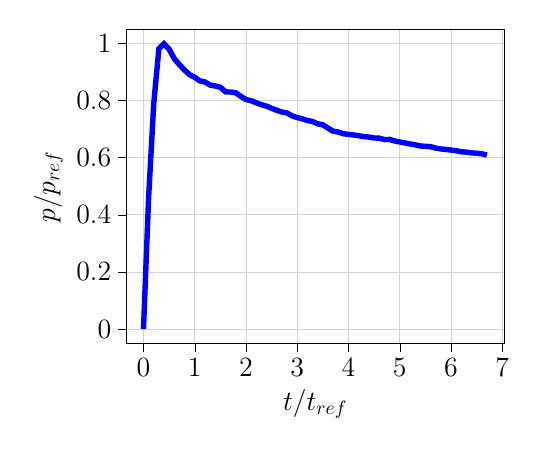
\begin{tikzpicture}[scale=0.7, font=\Large]

\definecolor{lightgray}{RGB}{211,211,211}

\begin{axis}[
tick align=outside,
tick pos=left,
x grid style={lightgray},
xlabel={\(\displaystyle t/t_{ref}\)},
xmajorgrids,
xmin=-0.335, xmax=7.035,
xtick style={color=black},
y grid style={lightgray},
ylabel={\(\displaystyle p/p_{ref}\)},
ymajorgrids,
ymin=-0.0498825329280283, ymax=1.0475331914886,
ytick style={color=black}
]
\addplot [line width=2.8pt, blue]
table {%
0 0
0.1 0.45951217560765
0.2 0.788592266536983
0.3 0.979658043857808
0.4 0.997650658560567
0.5 0.978785067303964
0.6 0.945971757956235
0.7 0.924877167218727
0.8 0.905966129538245
0.9 0.889602759640749
1 0.880357526928354
1.1 0.867671216379265
1.2 0.864233448832077
1.3 0.853114312789821
1.4 0.850108135287821
1.5 0.845620481022948
1.6 0.829505321551291
1.7 0.82892647153026
1.8 0.826514080553166
1.9 0.813655142687903
2 0.802768783688767
2.1 0.798543387344519
2.2 0.791408224631453
2.3 0.784592950157044
2.4 0.779669735090534
2.5 0.771982941261582
2.6 0.764935123584626
2.7 0.759180136109881
2.8 0.755819802453577
2.9 0.745394700232725
3 0.739759343297616
3.1 0.73509236716247
3.2 0.729345702728615
3.3 0.725778734141958
3.4 0.717687645906032
3.5 0.714371573361759
3.6 0.702688940886406
3.7 0.692071117257683
3.8 0.689075788412169
3.9 0.683018346545578
4 0.680940241480926
4.1 0.678761582675207
4.2 0.676155909908243
4.3 0.67303862482668
4.4 0.67141982291266
4.5 0.668213339195578
4.6 0.667744559568312
4.7 0.662721346127251
4.8 0.663129635213632
4.9 0.657892335911165
5 0.654296951897791
5.1 0.650863757765831
5.2 0.647428666367983
5.3 0.644241597549297
5.4 0.640318013987773
5.5 0.638947287170507
5.6 0.638052591816986
5.7 0.632877744620429
5.8 0.629874714646489
5.9 0.62812562862508
6 0.625989632848015
6.1 0.623727478456361
6.2 0.61994558051626
6.3 0.618837276024664
6.4 0.616144894474259
6.5 0.614945973289227
6.6 0.612979236533847
6.7 0.60828213805131
};
\end{axis}

\end{tikzpicture}
\hspace{0.5cm}
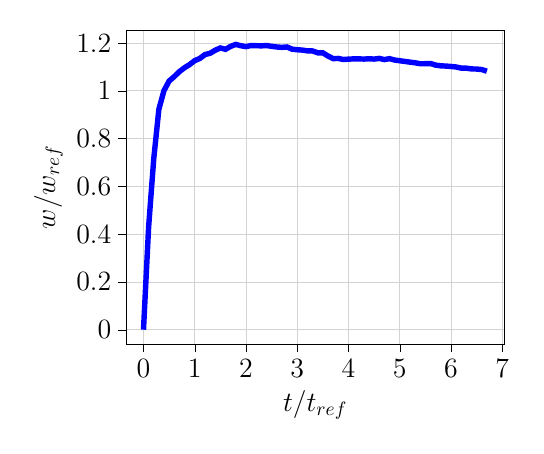
\begin{tikzpicture}[scale=0.7, font=\Large]

\definecolor{lightgray}{RGB}{211,211,211}

\begin{axis}[
tick align=outside,
tick pos=left,
x grid style={lightgray},
xlabel={\(\displaystyle t/t_{ref}\)},
xmajorgrids,
xmin=-0.335, xmax=7.035,
xtick style={color=black},
y grid style={lightgray},
ylabel={\(\displaystyle w/w_{ref}\)},
ymajorgrids,
ymin=-0.0597293287257296, ymax=1.25431590324032,
ytick style={color=black}
]
\addplot [line width=2.8pt, blue]
table {%
0 0
0.1 0.42960065054532
0.2 0.715136605775466
0.3 0.922750840112107
0.4 1.0013207791429
0.5 1.0411598779676
0.6 1.05982581607324
0.7 1.08050584575762
0.8 1.09671277193648
0.9 1.11032136558952
1 1.12663033076329
1.1 1.13590704337549
1.2 1.15199446917512
1.3 1.15745805434228
1.4 1.17029484955157
1.5 1.1797256365628
1.6 1.17401971466754
1.7 1.18622756700584
1.8 1.19458657451459
1.9 1.18892597827636
2 1.18545966357443
2.1 1.18983889045998
2.2 1.18920351864721
2.3 1.18850491342986
2.4 1.18987192915262
2.5 1.18655089416824
2.6 1.18376216613162
2.7 1.18232996709817
2.8 1.18384178574721
2.9 1.1745917982695
3 1.17218634899917
3.1 1.17081354140302
3.2 1.1674404732521
3.3 1.16714196039589
3.4 1.15942128056545
3.5 1.15905443325056
3.6 1.14598602032622
3.7 1.13512321674529
3.8 1.13577811166775
3.9 1.13137169873407
4 1.13287911123356
4.1 1.13401684532316
4.2 1.13401065495831
4.3 1.13319092621984
4.4 1.13446327534522
4.5 1.13314924992658
4.6 1.13590775886393
4.7 1.13102049244932
4.8 1.13486709640336
4.9 1.12912798009531
5 1.12617496099899
5.1 1.12326496239068
5.2 1.1202902089975
5.3 1.11761318780537
5.4 1.11361031173121
5.5 1.11379000169957
5.6 1.11459022130972
5.7 1.10788856842442
5.8 1.1048189314348
5.9 1.10389204151723
6 1.10216294677504
6.1 1.10006683973921
6.2 1.09525678021556
6.3 1.09503757716002
6.4 1.09193800888068
6.5 1.09139905221393
6.6 1.08928999986265
6.7 1.08233446321413
};
\end{axis}

\end{tikzpicture}
\caption{Two quantities of interest for the merging fracture problem. On the left, the time series of the pressure at the injection point, on the right, the fracture aperture. Both plots show results scaled by reference values, calculated at the onset of propagation.}  
\label{fig:merging_charts}
\end{figure}


\begin{figure}[h]
\begin{subfigure}{.45\textwidth}
  \centering
  \includegraphics[width=\linewidth]{Chapter4/figures/merging/merging_t_1.png}
  \caption{}
  \label{fig:merge_t_0}
\end{subfigure}%
\hspace{1cm}
\begin{subfigure}{.45\textwidth}
  \centering
  \includegraphics[width=\linewidth]{Chapter4/figures/merging/merging_t_14.png}
  \caption{}
  \label{fig:merge_t_1}
\end{subfigure}%

\begin{subfigure}{.45\textwidth}
  \centering
  \includegraphics[width=\linewidth]{Chapter4/figures/merging/merging_t_27.png}
  \caption{}
  \label{fig:merge_t_2}
\end{subfigure}
\hspace{0.85cm}
\begin{subfigure}{.45\textwidth}
  \centering
  \includegraphics[width=\linewidth]{Chapter4/figures/merging/merging_t_35.png}
  \caption{}
  \label{fig:merge_t_3}
\end{subfigure}

\begin{subfigure}{.45\textwidth}
  \centering
  \includegraphics[width=\linewidth]{Chapter4/figures/merging/merging_t_42.png}
  \caption{}
  \label{fig:merge_t_4}
\end{subfigure}
\hspace{0.85cm}
\begin{subfigure}{.45\textwidth}
  \centering
  \includegraphics[width=\linewidth]{Chapter4/figures/merging/merging_t_67.png}
  \caption{}
  \label{fig:merge_t_5}
\end{subfigure}
  \caption{Snapshots of the simulated propagation. The discrete fracture is colored in grayscale according to the aperture and the subdomain colored according the damage value. (a) Snapshot $t/t_{ref} = 0$; (b) $t/t_{ref} = 1.3$; (c) $t/t_{ref} = 2.6$; (d) $t/t_{ref} = 3.9$; (e) $t/t_{ref} = 5.2$; and (f) $t/t_{ref} = 6.5$. } 
  \label{fig:merge_snapshots}  
\end{figure}

\FloatBarrier




%==============================================================================

%-----------------------------------------------------------------------------%
% APPENDICES -- OPTIONAL. These are just chapters enumerated by Appendix A,
%                Appendix B, Appendix C...
%-----------------------------------------------------------------------------%
%\appendix
%\chapter{Extending the Multi-Resolution Approach to Three Dimensions}
\label{section: Chapter4}

\section{Introduction}
\label{section: Chapter4/intro}

Although two-dimensional simulations based on the multi-resolution algorithm proposed in the previous chapter can be useful to study fundamental processes in hydraulic fracturing, realistic systems are almost always three-dimensional. %Therefore, an extension of the approach to 3D is certainly the most natural next step to be taken. 
Accordingly, this chapter proposes a new propagation algorithm for the multi-resolution approach that is suited for planar fractures in three dimensions. This algorithm is implemented in the HPC solver GEOS \cite{settgast2012simulation,settgast2014simulation,settgast2017fully} through a collaboration with Lawrence Livermore National Laboratory. 

The chapter begins with a brief summary of the multi-resolution algorithm and then moves to the detailed description of the new propagation algorithm for the case of planar fractures. Illustrative examples are presented, including in-plane merging of two-penny shaped cracks. In the end, in Section \ref{section: Chapter4/nonplanar}, the extension to non-planar fractures in 3D is discussed, and the prototype of an algorithm is presented. A simplified version of this algorithm is implemented and tested in a 2.5D problem with a curved crack. Finally, the extension to more general fracture problems is discussed.  

%While it addresses some of the challenges, it requires further work to handle the general case.

\section{Theory}
\label{section: Chapter4/theory}

In Chapter \ref{section: Chapter3}, the mathematical model for single-phase fluid-driven fracture is described in Section \ref{formulation}. In what follows, this same model is assumed, as all derivations are independent of the system dimensionality as well as fracture shapes. More precisely, since the multi-resolution framework will be used, two coexisting descriptions are used. In a global domain, cracks are assumed to be represented by two-dimensional surfaces embedded in the 3D domain and the governing equations and boundary condition are those from \eqref{linear momentum balance} - \eqref{pf_ic}, which assume a fixed fracture geometry. In the local domain, which will be described next, the fracture problem is treated with a variational phase-field formulation, given by \eqref{basic u problem}-\eqref{eq:ddot-strong} which assume flow quantities to be fixed.

A more detailed discussion of the motivation and fundamentals of the multi-resolution method is provided in Section \ref{numerics}. In a nutshell, it breaks a fracture problem in two separate problems. In the global one, that covers the whole domain, a discrete representation of the fracture is used, but its geometry is assumed to be fixed. To account for crack propagation, a local problem in a vicinity of the fracture front is set up, employing the phase-field method, taking advantage of its flexibility in representing evolving fracture geometries.

This type approach is particularly interesting for simulating fluid-driven fracture due to the presence of a discrete fracture in the global level, which simplifies the computation of the fracture apertures that must be coupled to the fluid problem. If a pure phase-field description is used, extracting these apertures becomes a challenging task. In addition to that, a multi-resolution approach can also alleviate the computational cost that comes with the high-refined grids needed to solve phase-field problems. This becomes a remarkable limitation in the context of hydraulic fracturing since the length of fractures is usually of the order of kilometers.

An attentive reader will realize that the multi-resolution algorithm proposed in Chapter \ref{section: Chapter3} is not easily extendable to three-dimensions only because of the propagation step described in the subsection \ref{propagation_step}. In this part of the algorithm, a crack tip location is extracted from the damage field in the local problem and used to inform the global problem how to advance the crack. The concept of a crack tip does not exist in three-dimensions (it becomes a fracture front). In addition to that, while in 2D it is possible to connect line cuts (which are just line segments) to form an approximation to the crack geometry, in 3D these become planar cuts, which may fail to connect on element boundaries. SHOW FIGURE. 

The first extension discussed in this chapter deals with the case of planar fractures in 3D. The main challenge here consists of tracking the entire fracture front and evolving it according to the damage field computed in the local problem. This is done defining a discrete set of crack front elements which are investigated for damage throughout the problem execution. The construction of this layer of front elements ahead of the crack prevents is important to preserve the accuracy of the solution, because the lack fluid flow in the local problem can lead to spurious unstable solutions.

For the more complex case of non-planar fracture propagation, some considerations will be discussed in section \ref{}. The prototype of an algorithm to handle this case will be shown together with some preliminary results. However, it's robustness is not guaranteed. 

algorithm summary and figures

some results xda

\begin{figure}[h]
    \centering
    \includegraphics[width=0.5\linewidth]{Chapter4/figures/blue_circle.png}
    \caption{Multi-resolution solution algorithm.}
    \label{fig:lorem1}
\end{figure}


\begin{figure}[h]
    \centering
    \includegraphics[width=\linewidth]{Chapter4/figures/penny_with_descriptions.png}
    \caption{Multi-resolution solution algorithm.}
    \label{fig:lorem4}
\end{figure}

\begin{figure}[h]
    \centering
    \includegraphics[width=\linewidth]{Chapter4/figures/penny_with_descriptions.png}
    \caption{Multi-resolution solution algorithm.}
    \label{fig:lorem4}
\end{figure}

\begin{figure}[h]
    \centering
    \includegraphics[width=\linewidth]{Chapter4/figures/larger_penny_with_descriptions.png}
    \caption{Multi-resolution solution algorithm.}
    \label{fig:lorem2}
\end{figure}

\begin{figure}[h]
    \centering
    \includegraphics[width=0.5\linewidth]{Chapter4/figures/larger_penny.png}
    \caption{Multi-resolution solution algorithm.}
    \label{fig:lorem3}
\end{figure}

\begin{figure}[h]
    \centering
    \includegraphics[width=\linewidth]{Chapter4/figures/planar3D_algorithm.png}
    \caption{Multi-resolution solution algorithm.}
    \label{fig:lorem5}
\end{figure}


\section{Algorithm for planar fractures}
\label{section: Chapter4/algo}

\begin{figure}[h]
    \centering
    \includegraphics[width=\linewidth]{Chapter4/figures/planar3D_algorithm.png}
    \caption{Multi-resolution solution algorithm.}
    \label{fig:MR_planar_algo}
\end{figure}

A high-level description of the propagation algorithm for planar fractures in 3D is shown in Figure \ref{fig:MR_planar_algo}. It summarizes each of the steps involved in the solution procedure for a single time-setp. The process begins with the solution of the global problem (i.e, the box colored in blue in \ref{fig:MR_planar_algo}). As pointed out in chapter \ref{section: Chapter3}, the algorithm is agnostic with respect to the numerical methods employed. The approximate fields for pressure and displacements are then transfered to the local problem, as explained in the steps (3) and (4) of Algorithm \ref{fig:solution_algorithm}.

In the 2D algorithm, one would now move to the solution of the local problem with an alternate minimization approach and only then check for fracture propagation. In the proposed 3D algorithm, this is changed and a damage tracking function is launched in parallel with the damage solver. This function checks the amount of damage in the elements of the fracture from (which is described in detail in subsection \ref{sec:front}). Different measurements of damage can be employed, and they will likely depend on the discretization method employed. A simple one, which works well for planar fractures in structured grids is the volume of damage, which is defined as the total volume of subdiscretization' elements with damage above a threshold (usually around 0.9). This approach is effective since, for planar fractures aligned with structured grids, the fracture area on each element can be predicted beforehand. This simpliefied criteria is used in the example problems shown in Section \ref{section: Chapter4/examples}. It is discussed in more detail, together with a more general approach in subsection \ref{frontTrackingAlgo}.

If any of the front elements is identified as being cracked (i.e, the level of damage on it is very high), the alternate minimization iterations are halted. The geometry of the discrete fracture in the global is then updated. This update consists of the addition of a planar cut in this cracked element, followed by an advance in the fracture front. This in turns lead to an advance in the local domain.

If multiple front elements are cracked, this process is done for all of them. The current time-step is then re-launched. Convergence is achieved when the alternate minization procedure reaches a prescribed tolerance without triggering the fracture propagation. When that happens, an equilibrium state is obtained and the time-step can be advanced.

\subsection{Fracture front construction}\label{sec:front}

The fracture front plays an important role in the propagation step. It greatly reduces the computational expense associated with the inspection of damage in the global elements while also serving to indicate a reference position to place the subdomains as the crack advances. It's construction happens during the initial discretization of the fracture in the global domain. One goes over all fractured elements and among its neighbors, adding to the front those elements that share a fractured face (but are not yet fractured) with the fractured ones (Figure XX). This step is repeated every time the global fracture geometry is updated (i.e new fracture cells are inserted). Figure \ref{fig:crack_front} shows the fracture front for a penny shaped crack. Figure \ref{fig:crack_prop_steps} shows the sequence of steps involved in the fracture propagation process, including the update of the fracture front.

\begin{figure}[h]
    \centering
    \includegraphics[width=0.4\linewidth]{Chapter4/figures/front_penny.png}
    \caption{Penny shaped crack discretized in a coarse grid. Red elements represent the fractured elements (which contain EFEM enrichments). The fracture front elements are shown in green. }
    \label{fig:crack_front}
\end{figure}

\begin{figure}
    \floatsetup[subfigure]{style=plain,capposition = beside, capbesideposition={left, center},capbesidesep=quad, capbesidewidth =5cm, captionskip=20pt, rowpostcode=captionskip}
    \captionsetup[subfloatrow]{format=hang, labelfont=up, textfont=up}
    \captionsetup{labelfont=sc, textfont = it}
    \ffigbox{%
      \begin{subfloatrow}[1]
        \fcapside{\caption{Beginning of time step. The phase-field fracture is shown as a countor to facilitate the visualization. As in \ref{fig:crack_front}, green elements represent the front and red the discrete fracture.}}
        {\includegraphics[width=\linewidth]{Chapter4/figures/penny_with_descriptions.png}}
      \end{subfloatrow}\\
      \begin{subfloatrow}[1]
        \fcapside{\hspace*{0.25cm}\includegraphics[width=0.9\linewidth]{Chapter4/figures/larger_penny_with_descriptions.png}}
        {\caption{After a few iterations in the local problem, the phase-field advances and some front elements (now in orange) are identified as fully damaged. They will be fractured and their neighbors in light green will be added to the front.}}
      \end{subfloatrow}\\
      \begin{subfloatrow}[1]
        \fcapside{\hspace*{2.60cm}\includegraphics[width=0.6\linewidth]{Chapter4/figures/larger_penny.png}}
        { \caption{Final configuration after the updates. Since the global fracture changed, the time-step must be relaunched.}}
      \end{subfloatrow}\\
      }{\caption{Sequence of steps performed during crack propagation.}
      \label{fig:crack_prop_steps}}
  \end{figure}

% \begin{figure}[h]
% %    \begin{subfigure}

%         \floatbox[{\capbeside\thisfloatsetup{capbesideposition={left,top},capbesidewidth=4cm}}]{figure}[\FBwidth]
%         {\caption{Beginning of time step. The phase-field fracture is shown as a countor to facilitate the visualization. As in \ref{fig:crack_front}, green elements represent the front and red the discrete fracture.}}
%         {\includegraphics[width=5cm]{Chapter4/figures/penny_with_descriptions.png}}
%         % \hspace*{1.85cm}\includegraphics[scale = 0.9, width=0.55\linewidth]{Chapter4/figures/penny_with_descriptions.png}
%         % \caption{Beginning of time step. The phase-field fracture is shown as a countor to facilitate the visualization. As in \ref{fig:crack_front}, green elements represent the front and red the discrete fracture.}
%         % \label{fig:lorem1}
% %    \end{subfigure}
% \end{figure}
% \begin{figure}[h]
%     \begin{subfigure}{\textwidth}    
%         \hspace*{2.35cm}\includegraphics[scale = 0.9, width=0.51\linewidth]{Chapter4/figures/larger_penny_with_descriptions.png}
%         \caption{After a few iterations in the local problem, the phase-field advances and some front elements (now in orange) are identified as fully damaged. They will be fractured and their neighbors in light green will be added to the front.}
%         \label{fig:lorem2}
%     \end{subfigure}
    
%     \begin{subfigure}{\textwidth}
%         \centering
%         \includegraphics[scale = 0.9, width=0.33\linewidth]{Chapter4/figures/larger_penny.png}
%         \caption{Final configuration after the updates. Since the global fracture changed, the time-step must be relaunched.}
%         \label{fig:lorem3}
%     \end{subfigure}
%     \caption{Sequence of steps performed during crack propagation.}
%     \label{fig:crack_prop_steps}
% \end{figure}

\FloatBarrier

\subsection{Tracking damage in the fracture front elements}\label{frontTrackingAlgo}

The process of tracking the damage in the front elements also deserves a more detailed explanation. First, a simplified criterion suitable for planar cracks in structured grids is detailed. This is the one that is used in the preliminary results shown next. Then, a more general approach that can be used for unstructured meshes is described.

\subsubsection{Volume of damage criterion}

For this criterion, consider a structured grid, aligned with the coordinate axis and with the fracture planes. Suppose that a given element in the global domain has has dimensions $H_x, H_y$ and $H_z$ whereas the local one has $h_x, h_y$ and $h_z$.

Ths criterion begins by first computing the cross sectional area of that element along the fracture plane. For example, for a fracture whose normal is in the x direction, one gets $H_yH_z$. This is only possible when the structured grid is aligned with the fracture (either in $x, y$ or $z$).

Then, assuming that the fully damaged region of a phase-field fracture consists of a single element across the damage band width, the volume of the fully-cracked region can be estimated to be $h_xH_yH_z$ when the damage complete crosses the elemeent. So, to check if that has happened, the volume of local elements with damage above a threshold (consider 0.9) is computed from the local problem solution. A global element is then considered fractured if this volume reaches $h_xH_yH_z$.

This method contains multiple limitations, such as the need for planar fractures aligned with a structured grid and also the hypothesis that the damage band has a single fully degraded element along its width. However, in many practical applications, the fractures are indeed assumed to be parallel to each other and structured grids are also prefered, as they can substantially reduce memory use. 

\subsubsection{Topological criterion}

An alternative method to circunvent these limitation is inspired by \cite{muixi2021combined}. It consists of evaluating the damage field in the edges of an element. It assumes that a fractured element has at least three fractured faces and that a fractured face is cut on two of its edges.

For each global element in the crack front, the damage field, computed in the local mesh, is inspected on every edge. If damage above a threshold (typically 0.9 or 0.95) is identified in a given edge, that edge is considered cut. If any face contains two cut edges, it is marked as cut. An element is then marked as fracture when at least three of its faces are cut.

This criteria circunvents some of the limitations of the simpliefied one, removing the need for structured grids. It is also applicable to nonplanar fractures as well. However, it is not perfectly robust and certain relative configurations between the damage field and the global element in the front can lead to unexpected results. This will be shown in Section \ref{section: Chapter4/nonplanar} that discusses the case of nonplanar fractures.


% \begin{figure}[h]
%     \centering
%     \begin{subfigure}{.45\textwidth}
%         \centering
%         \includegraphics[width=\linewidth]{Chapter4/figures/penny_with_descriptions.png}
%         \caption{Multi-resolution solution algorithm.}
%         \label{fig:lorem1}
%     \end{subfigure}%
%     \begin{subfigure}{.45\textwidth}
%         \centering
%         \includegraphics[width=\linewidth]{Chapter4/figures/penny_with_descriptions.png}
%         \caption{Multi-resolution solution algorithm.}
%         \label{fig:lorem2}
%     \end{subfigure}%
    
%     \bigskip
%     \begin{subfigure}{.45\textwidth}
%         \centering
%         \includegraphics[width=\linewidth]{Chapter4/figures/larger_penny_with_descriptions.png}
%         \caption{Multi-resolution solution algorithm.}
%         \label{fig:lorem3}
%     \end{subfigure}
%     \begin{subfigure}{.45\textwidth}
%         \centering
%         \includegraphics[width=0.65\linewidth]{Chapter4/figures/larger_penny.png}
%         \caption{Multi-resolution solution algorithm.}
%         \label{fig:lorem4}
%     \end{subfigure}
%       \caption{Schematic of propagation steps.}
% \end{figure}

% \begin{figure}[h]
%     \centering
%     \begin{subfigure}{\textwidth}
%         \centering
%         \includegraphics[width=\linewidth]{Chapter4/figures/penny_with_descriptions.png}
%         \caption{Multi-resolution solution algorithm.}
%         \label{fig:lorem1}
%     \end{subfigure}%
%     \bigskip
%     \begin{subfigure}{\textwidth}
%         \centering
%         \includegraphics[width=\linewidth]{Chapter4/figures/larger_penny_with_descriptions.png}
%         \caption{Multi-resolution solution algorithm.}
%         \label{fig:lorem2}
%     \end{subfigure}
%     \bigskip
%     \begin{subfigure}{\textwidth}
%         \centering
%         \includegraphics[width=0.65\linewidth]{Chapter4/figures/larger_penny.png}
%         \caption{Multi-resolution solution algorithm.}
%         \label{fig:lorem3}
%     \end{subfigure}
%     \caption{Schematic of propagation steps.}
% \end{figure}





\section{GEOS Implementation}
\label{section: Chapter4/implementation}

Test implementation section.

\section{Numerical examples}
\label{section: Chapter4/examples}

In this Section, a two example problems computed with the aforementioned method are presented. These examples illustrate the main capabilities of the approach, but also serve to demonstrate some of the limitations. They all consist of hydrulic fracture propagation in a poroelastic medium involving different fracture configurations that are relevant to practical fracking applications. The main goal is to ensure that the proposed algorithm supports these two representative scenarios and that it can be used to simulate real world fracking treatments whenever the assumption of planar growth is adequate. 

Importantly, a true verification procedure is not performed here. For example, mesh convergence studies and comparisons with well-known solutions are yet to be performed for these 3D problems as we did in Chapter \ref{section: Chapter3}. These require a few enhancements in the solver technology that are currently under development. First, due to the high discrepancy between the scales of degrees of freedom (matrix displacements, fracture apertures and pressures), general purpose linear solvers struggle to converge when the meshes are refined past a certain point. Because of that, special preconditioners that take into account the block structure of the system are being developed. Second, analytical solutions for poroelastic problems are scarce, so, a common verification procedure consists in solving them with vanishing small permeability coefficients to verify convergence towards the impermeable case, which does have a closed-form solution. However, as the permeability decreses, the poromechanics problem starts to display spurious pressure oscillations unless LBB-stable elements \cite{arnold1984stable} or a stabilized formulations, such as \cite{white2008stabilized} are used. These enhancements in the solver infrastructure are left for future work.

For the two problems in this Section, the material properties used are listed in Table \ref{material properties ch4}. The fluid injection rate $Q$ is set to $2.0 m^3/s$ (on each injection point).

\begin{table}[h]
  \centering
  \caption{Material properties for planar fracture problems.}
  \begin{tabular}[t]{lcc}
  \hline
  &Value &Unit \\
  \hline
  Young's modulus ($E$)&16.0&GPa\\
  Poisson's ratio ($\nu$)&0.18&--\\
  Fluid viscosity ($\mu$)&1.0$\times10^{-12}$&$\text{GPa . s}$\\
  Fluid bulk modulus ($K_f$)&1.0$\times10^{10}$&$\text{GPa}$\\
  Critical energy release rate ($G_c$)&2.5&$\text{N/m}$\\
  Biot coefficient ($\alpha$)&1.0&$\text{ - }$\\
  Rock permeability ($\kappa_0$)&1.0$\times 10^{-13}$&$\text{m}^2$\\
  Initial porosity ($\phi_0$)&0.2&$\text{-}$\\
  \hline
  \end{tabular}
  \label{material properties ch4}
\end{table}%

\subsection{Two parallel circular fractures under fluid injection}

In the first problem, a pair of parallel penny-shaped fractures is stimulated with the injection of a viscous fluid. This configuration is representative of a very common scenario in real-world fracking treatments where, in general, there are multiple clusters with several parallel fractures in each. Their simultaneous stimulation can lead to all fractures growing simultaneously or to situations in which only a few show substantial propagation while the others arrest early in the process. These scenarios can lead to very different well behaviors.   

Depending on the distance between the fractures, there may also be non-planar growth, with fractures propagating away from each other, forming a cup shaped geometry. This is a consequence of the interaction between the stress fields in the vicinity of the multiple fractures fronts. This interaction is often called stress shadow effect. In this numerical example shown here, the initial fractures are placed far from each other to prevent this non-planar behavior. The far-field boundary conditions are assumed to be homogenous for pressures and displacements. Figure \ref{fig:parallel_schematic} illustrates the geometry. The dimensions are described in Table \ref{parallel_measures}.

As for the discretization, the coarser global mesh consists of a structured grid that is refined near the fracture planes, with an element size of around 0.075m in the width direction and 0.15m in the other directions. The local mesh is 5 times smaller and the regularization length used in the phase-field subproblem is 0.05m. Importantly, the local domain consists of all local elements within a distance of 1m to the fracture front. Since the fractures are penny shaped, this local domain will have the shape of a torus. As for the time-step, it is uniformly set to 0.01s.

Due to the uniform boundary conditions and homogenous material properties, the fractures are expected to grow radially, preserving their circular shape. This feature is confirmed in the simulated results shown in Figure \ref{fig:parallel_snapshots}. In these snapshots, the right-side of the domain shows the pressure field computed in the global domain whereas the left side shows the discrete crack geometry, colored in gray scale indicating the aperture field. This figure also shows the subdomain around the crack front, colored by the damage field.

The aperture and pressure at the injection sources are important quantities of interest in this type of problem and their simulated time series are shown in Figure \ref{fig:parallel_fracs_charts}. Due to the symmetry, both fractures have the same pressure and aperture results. The reference values used to make the curves nondimensional are listed in Table \ref{parallel_refs}.

\begin{table}[ht]
  \centering
  \caption{Domain dimensions}
  \begin{tabular}[t]{lccccccc}
  \hline
  &$d_1$&$d_2$&$d_3$&$L_x$&$L_y$&$L_z$&$r$\\  
  \hline
  Value (m) & 4.0 & 8.0 & 4.0 & 16.0 & 5.0 & 5.0 & 1.3\\
  \hline
  \end{tabular}
  \label{parallel_measures}
\end{table}%

\begin{table}[ht]
  \centering
  \caption{Reference values used in the time series plots.}
  \begin{tabular}[t]{lcc}
  \hline
  &Value &Unit \\
  \hline
  $p_{ref}$&$320$&MPa\\
  $w_{ref}$&$5.0\times10^{-4}$&m\\
  $t_{ref}$&$10$&$\text{s}$\\
  \hline
  \end{tabular}
  \label{parallel_refs}
\end{table}%

\begin{figure}[ht]
  \centering
  \begin{tikzpicture}
      \node {\pgfimage[interpolate=false,width=0.8\textwidth]{Chapter4/figures/3D/parallel_schematic.png}};
      \draw (-0.11\textwidth,0.185\textwidth) node {\large$r$};
      \draw (0.3\textwidth,0.12\textwidth) node {\large$L_x$};
      \draw (0.1\textwidth,-0.31\textwidth) node {\large$L_y$};
      \draw (0.42\textwidth,-0.15\textwidth) node {\large$L_z$};
      \draw (-0.05\textwidth,0.3\textwidth) node {\large$d_1$};
      \draw (0.02\textwidth,0.23\textwidth) node {\large$d_2$};
      \draw (0.09\textwidth,0.15\textwidth) node {\large$d_3$};
  \end{tikzpicture}
  \caption{Schematic of the problem geometry.}
  \label{fig:parallel_schematic}
\end{figure}


\begin{figure}[h]
  \noindent% This file was created with tikzplotlib v0.10.1.
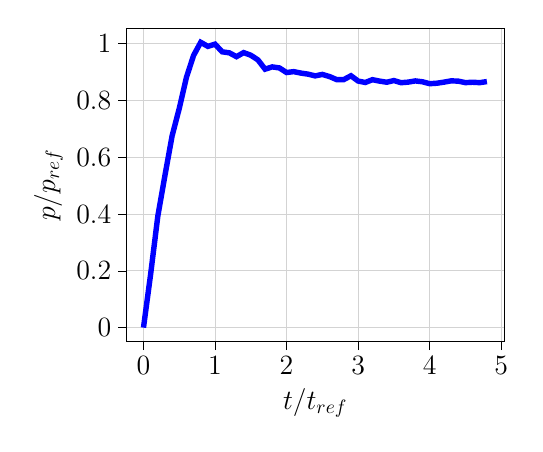
\begin{tikzpicture}[scale=0.7, font=\Large]

\definecolor{lightgray}{RGB}{211,211,211}

\begin{axis}[
tick align=outside,
tick pos=left,
x grid style={lightgray},
xlabel={\(\displaystyle t/t_{ref}\)},
xmajorgrids,
xmin=-0.24, xmax=5.04,
xtick style={color=black},
y grid style={lightgray},
ylabel={\(\displaystyle p/p_{ref}\)},
ymajorgrids,
ymin=-0.0502281761912294, ymax=1.05479170001582,
ytick style={color=black}
]
\addplot [line width=2.8pt, blue]
table {%
0 0
0.1 0.188445766752718
0.2 0.391947508110223
0.3 0.535895204930158
0.4 0.675176372415468
0.5 0.771710290038251
0.6 0.880899367078848
0.7 0.958412412909037
0.8 1.00456352382459
0.9 0.990324948221893
1 0.998054606057314
1.1 0.971102817197564
1.2 0.967556258546069
1.3 0.954084839144053
1.4 0.968359167181806
1.5 0.959116405852193
1.6 0.942617944583139
1.7 0.910026091662552
1.8 0.918049400613525
1.9 0.914348525898006
2 0.898192078875057
2.1 0.901362856789026
2.2 0.896214438996315
2.3 0.892511564645737
2.4 0.886358846124087
2.5 0.891502924804546
2.6 0.884023936770732
2.7 0.873345919605794
2.8 0.873412882862689
2.9 0.886829564180904
3 0.868198311002277
3.1 0.863129333961807
3.2 0.873000347785484
3.3 0.867964509851173
3.4 0.864042793812506
3.5 0.869939165930708
3.6 0.862387111210862
3.7 0.864402846886308
3.8 0.868605632794512
3.9 0.865597652226709
4 0.8589197342603
4.1 0.860522133055493
4.2 0.864358319941601
4.3 0.868875836425173
4.4 0.867843224744737
4.5 0.862641238764823
4.6 0.863963070087864
4.7 0.862565672752955
4.8 0.866328855022948
};
\end{axis}

\end{tikzpicture}

  \hspace{0.5cm}
  % This file was created with tikzplotlib v0.10.1.
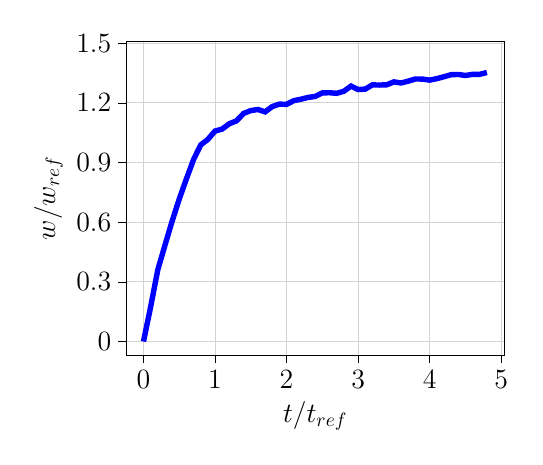
\begin{tikzpicture}[scale=0.7, font=\Large]

\definecolor{lightgray}{RGB}{211,211,211}

\begin{axis}[
tick align=outside,
tick pos=left,
x grid style={lightgray},
xlabel={\(\displaystyle t/t_{ref}\)},
xmajorgrids,
xmin=-0.24, xmax=5.04,
xtick style={color=black},
y grid style={lightgray},
ytick distance=0.3,
ylabel={\(\displaystyle w/w_{ref}\)},
ymajorgrids,
ymin=-0.0676150128188689, ymax=1.51,
ytick style={color=black}
]
\addplot [line width=2.8pt, blue]
table {%
0 0
0.1 0.174099460537345
0.2 0.36037093622801
0.3 0.483736302329922
0.4 0.604657400483929
0.5 0.71627362525909
0.6 0.817741763252065
0.7 0.914673087058184
0.8 0.988043835003288
0.9 1.01615749619579
1 1.05781999647227
1.1 1.06795558571426
1.2 1.09487671410362
1.3 1.10903211791217
1.4 1.14665606861212
1.5 1.16093104459679
1.6 1.16625499737314
1.7 1.15430886393875
1.8 1.18121700420342
1.9 1.19330912726223
2 1.19206895215774
2.1 1.21057291458408
2.2 1.21798236109138
2.3 1.22691783387849
2.4 1.23188777939765
2.5 1.24970648339836
2.6 1.25053556512246
2.7 1.24766343959738
2.8 1.2578584515492
2.9 1.28381515930564
3 1.26659534216305
3.1 1.26894556444263
3.2 1.29005564497642
3.3 1.28918001813621
3.4 1.29050708947248
3.5 1.30520754884353
3.6 1.29951568143079
3.7 1.30872862561227
3.8 1.31974418932991
3.9 1.31922767023963
4 1.31398053120865
4.1 1.32143831069796
4.2 1.33095372857038
4.3 1.34126355648886
4.4 1.34234868328863
4.5 1.33716954069027
4.6 1.34310704227726
4.7 1.34310814299716
4.8 1.35230025637738
};
\end{axis}

\end{tikzpicture}

  \caption{Two quantities of interest for the parallel fracture problem. On the left, the time series of the pressure at the injection point, on the right, the fracture aperture. Both plots show results scaled by reference values, calculated at the onset of propagation.}  
  \label{fig:parallel_fracs_charts}
\end{figure}


\begin{figure}[h]
\begin{subfigure}{.45\textwidth}
  \centering
  \includegraphics[width=\linewidth]{Chapter4/figures/3D/new_t_0.png}
  \caption{}
  \label{fig:parallel_t_0}
\end{subfigure}%
\hspace{1cm}
\begin{subfigure}{.45\textwidth}
  \centering
  \includegraphics[width=\linewidth]{Chapter4/figures/3D/new_t_30.png}
  \caption{}
  \label{fig:parallel_t_1}
\end{subfigure}%

\begin{subfigure}{.45\textwidth}
  \centering
  \includegraphics[width=\linewidth]{Chapter4/figures/3D/new_t_60.png}
  \caption{}
  \label{fig:parallel_t_2}
\end{subfigure}
\hspace{0.85cm}
\begin{subfigure}{.45\textwidth}
  \centering
  \includegraphics[width=\linewidth]{Chapter4/figures/3D/new_t_90.png}
  \caption{}
  \label{fig:parallel_t_3}
\end{subfigure}
  \caption{Snapshots of the simulated propagation. The left side of the figures shows the discrete fracture colored in grayscale according to the aperture and the subdomain colored according the damage value. The right side shows the pressure field in the global domain. (a) Snapshot $t/t_{ref} = 0$; (b) $t/t_{ref} = 1.5$; (c) $t/t_{ref} = 3$; and (d) $t/t_{ref} = 4.5$. } 
  \label{fig:parallel_snapshots}
\end{figure}

\FloatBarrier

\subsection{Merging two circular fractures}

The second problem deals with the case of in-plane fracture merging. In general, fracture merging is one of the most difficult behaviors to simulate with discrete fracture approaches. That is due to the interaction between the stress fields of two fracture fronts, which makes most attempts to extract a stress intensity factor innacurate. In practice, these situation may happen when fracking wells are drilled parallel to each other. 

For problems involving crack merging, the phase-field approach becomes handy, allowing for the computation of crack advances through the solution of PDEs that are independent of the fracture topology.
The multi-resolution approach explore this advantage, keeping a phase-field description around the fracture front and removing the limitations of discrete methods.

Since this problem deals with in-plane merging, getting the discrete fracture planes from the phase-field values is straightforward. However, it is important to mention that this can be a challenge in the case of non-planar merging.

The problem under consideration consists of two parallel fractures, initally of circular shape, embedded in a poroelastic matrix. Both are injected with a viscous fluid and propagate radially, eventually merging. An schematic of the geometry is shown in Figure \ref{fig:merging_schematic}, with the dimensions listed in Table \ref{merging_measures}. As in the previous problem, the far-field boundary conditions are assumed to be homogenous for pressures and displacements. 

As for the discretization, the coarser global mesh consists of a structured grid that is refined near the fracture planes, with an element size of around 0.095m in the width direction and 0.15m in the other directions. The local mesh is 5 times smaller and the regularization length used in the phase-field subproblem is 0.05m. Importantly, the local domain consists of all local elements within a distance of 1m to the fracture front. Initally, they consist of two separate torus, but they eventually merge as the cracks get closer. As for the time-step, it is uniformly set to 0.01s.

The simulated behavior is depicted in Figure \ref{fig:merge_snapshots}, which shows the expected behavior, which the cracks growing perfectly as circles until they approach each other and merge. After the merge, the most concave part of the crack grows and opens up until the pressure drops enough for the propagation to arrest. While there is not reference solution to compare, at least qualitatively, the results make sense. As for the previous problem, the times series for the aperture and pressure in the injection point are shown in Figure \ref{fig:merging_charts}. The reference values used to make these charts nondimensional are given in Table \ref{merging_refs}.

\begin{table}[ht]
  \centering
  \caption{Domain dimensions}
  \begin{tabular}[t]{lccccccc}
  \hline
  &$d_1$&$d_2$&$d_3$&$L_x$&$L_y$&$L_z$&$r$\\  
  \hline
  Value (m) & 6.5 & 7.0 & 6.5 & 8.0 & 20.0 & 5.0 & 1.5\\
  \hline
  \end{tabular}
  \label{merging_measures}
\end{table}%

\begin{table}[ht]
  \centering
  \caption{Reference values used in the time series plots.}
  \begin{tabular}[t]{lcc}
  \hline
  &Value &Unit \\
  \hline
  $p_{ref}$&520&MPa\\
  $w_{ref}$&7.0$\times 10^{-4}$&m\\
  $t_{ref}$&10&$\text{s}$\\
  \hline
  \end{tabular}
  \label{merging_refs}
\end{table}%

\begin{figure}[ht]
  \centering
  \begin{tikzpicture}
      \node {\pgfimage[interpolate=false,width=.8\textwidth]{Chapter4/figures/merging/merging_schematic.png}};
      \draw (0.0\textwidth,0.07\textwidth) node {\large$r$};
      \draw (0.37\textwidth,0.12\textwidth) node {\large$L_x$};
      \draw (0.04\textwidth,-0.25\textwidth) node {\large$L_y$};
      \draw (0.42\textwidth,-0.07\textwidth) node {\large$L_z$};
      \draw (-0.25\textwidth,0.25\textwidth) node {\large$d_1$};
      \draw (-0.03\textwidth,0.25\textwidth) node {\large$d_2$};
      \draw (0.2\textwidth,0.25\textwidth) node {\large$d_3$};
  \end{tikzpicture}
  \caption{Schematic of the geometry for the merging problem.}
  \label{fig:merging_schematic}
\end{figure}


\begin{figure}[h]
\noindent% This file was created with tikzplotlib v0.10.1.
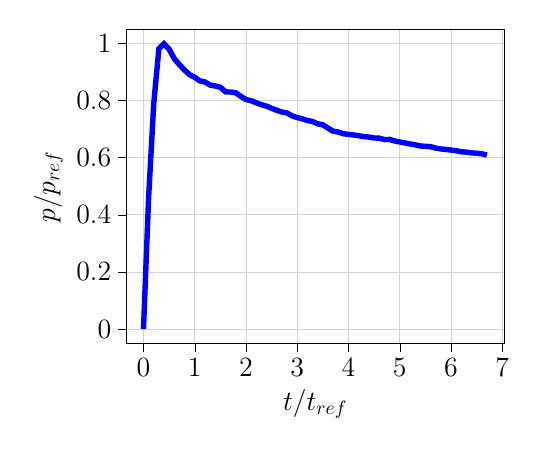
\begin{tikzpicture}[scale=0.7, font=\Large]

\definecolor{lightgray}{RGB}{211,211,211}

\begin{axis}[
tick align=outside,
tick pos=left,
x grid style={lightgray},
xlabel={\(\displaystyle t/t_{ref}\)},
xmajorgrids,
xmin=-0.335, xmax=7.035,
xtick style={color=black},
y grid style={lightgray},
ylabel={\(\displaystyle p/p_{ref}\)},
ymajorgrids,
ymin=-0.0498825329280283, ymax=1.0475331914886,
ytick style={color=black}
]
\addplot [line width=2.8pt, blue]
table {%
0 0
0.1 0.45951217560765
0.2 0.788592266536983
0.3 0.979658043857808
0.4 0.997650658560567
0.5 0.978785067303964
0.6 0.945971757956235
0.7 0.924877167218727
0.8 0.905966129538245
0.9 0.889602759640749
1 0.880357526928354
1.1 0.867671216379265
1.2 0.864233448832077
1.3 0.853114312789821
1.4 0.850108135287821
1.5 0.845620481022948
1.6 0.829505321551291
1.7 0.82892647153026
1.8 0.826514080553166
1.9 0.813655142687903
2 0.802768783688767
2.1 0.798543387344519
2.2 0.791408224631453
2.3 0.784592950157044
2.4 0.779669735090534
2.5 0.771982941261582
2.6 0.764935123584626
2.7 0.759180136109881
2.8 0.755819802453577
2.9 0.745394700232725
3 0.739759343297616
3.1 0.73509236716247
3.2 0.729345702728615
3.3 0.725778734141958
3.4 0.717687645906032
3.5 0.714371573361759
3.6 0.702688940886406
3.7 0.692071117257683
3.8 0.689075788412169
3.9 0.683018346545578
4 0.680940241480926
4.1 0.678761582675207
4.2 0.676155909908243
4.3 0.67303862482668
4.4 0.67141982291266
4.5 0.668213339195578
4.6 0.667744559568312
4.7 0.662721346127251
4.8 0.663129635213632
4.9 0.657892335911165
5 0.654296951897791
5.1 0.650863757765831
5.2 0.647428666367983
5.3 0.644241597549297
5.4 0.640318013987773
5.5 0.638947287170507
5.6 0.638052591816986
5.7 0.632877744620429
5.8 0.629874714646489
5.9 0.62812562862508
6 0.625989632848015
6.1 0.623727478456361
6.2 0.61994558051626
6.3 0.618837276024664
6.4 0.616144894474259
6.5 0.614945973289227
6.6 0.612979236533847
6.7 0.60828213805131
};
\end{axis}

\end{tikzpicture}
\hspace{0.5cm}
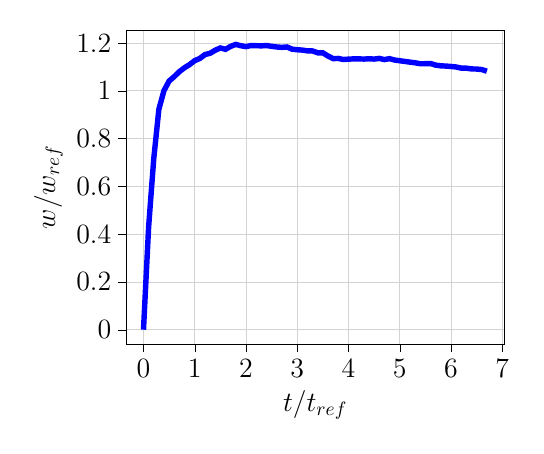
\begin{tikzpicture}[scale=0.7, font=\Large]

\definecolor{lightgray}{RGB}{211,211,211}

\begin{axis}[
tick align=outside,
tick pos=left,
x grid style={lightgray},
xlabel={\(\displaystyle t/t_{ref}\)},
xmajorgrids,
xmin=-0.335, xmax=7.035,
xtick style={color=black},
y grid style={lightgray},
ylabel={\(\displaystyle w/w_{ref}\)},
ymajorgrids,
ymin=-0.0597293287257296, ymax=1.25431590324032,
ytick style={color=black}
]
\addplot [line width=2.8pt, blue]
table {%
0 0
0.1 0.42960065054532
0.2 0.715136605775466
0.3 0.922750840112107
0.4 1.0013207791429
0.5 1.0411598779676
0.6 1.05982581607324
0.7 1.08050584575762
0.8 1.09671277193648
0.9 1.11032136558952
1 1.12663033076329
1.1 1.13590704337549
1.2 1.15199446917512
1.3 1.15745805434228
1.4 1.17029484955157
1.5 1.1797256365628
1.6 1.17401971466754
1.7 1.18622756700584
1.8 1.19458657451459
1.9 1.18892597827636
2 1.18545966357443
2.1 1.18983889045998
2.2 1.18920351864721
2.3 1.18850491342986
2.4 1.18987192915262
2.5 1.18655089416824
2.6 1.18376216613162
2.7 1.18232996709817
2.8 1.18384178574721
2.9 1.1745917982695
3 1.17218634899917
3.1 1.17081354140302
3.2 1.1674404732521
3.3 1.16714196039589
3.4 1.15942128056545
3.5 1.15905443325056
3.6 1.14598602032622
3.7 1.13512321674529
3.8 1.13577811166775
3.9 1.13137169873407
4 1.13287911123356
4.1 1.13401684532316
4.2 1.13401065495831
4.3 1.13319092621984
4.4 1.13446327534522
4.5 1.13314924992658
4.6 1.13590775886393
4.7 1.13102049244932
4.8 1.13486709640336
4.9 1.12912798009531
5 1.12617496099899
5.1 1.12326496239068
5.2 1.1202902089975
5.3 1.11761318780537
5.4 1.11361031173121
5.5 1.11379000169957
5.6 1.11459022130972
5.7 1.10788856842442
5.8 1.1048189314348
5.9 1.10389204151723
6 1.10216294677504
6.1 1.10006683973921
6.2 1.09525678021556
6.3 1.09503757716002
6.4 1.09193800888068
6.5 1.09139905221393
6.6 1.08928999986265
6.7 1.08233446321413
};
\end{axis}

\end{tikzpicture}
\caption{Two quantities of interest for the merging fracture problem. On the left, the time series of the pressure at the injection point, on the right, the fracture aperture. Both plots show results scaled by reference values, calculated at the onset of propagation.}  
\label{fig:merging_charts}
\end{figure}


\begin{figure}[h]
\begin{subfigure}{.45\textwidth}
  \centering
  \includegraphics[width=\linewidth]{Chapter4/figures/merging/merging_t_1.png}
  \caption{}
  \label{fig:merge_t_0}
\end{subfigure}%
\hspace{1cm}
\begin{subfigure}{.45\textwidth}
  \centering
  \includegraphics[width=\linewidth]{Chapter4/figures/merging/merging_t_14.png}
  \caption{}
  \label{fig:merge_t_1}
\end{subfigure}%

\begin{subfigure}{.45\textwidth}
  \centering
  \includegraphics[width=\linewidth]{Chapter4/figures/merging/merging_t_27.png}
  \caption{}
  \label{fig:merge_t_2}
\end{subfigure}
\hspace{0.85cm}
\begin{subfigure}{.45\textwidth}
  \centering
  \includegraphics[width=\linewidth]{Chapter4/figures/merging/merging_t_35.png}
  \caption{}
  \label{fig:merge_t_3}
\end{subfigure}

\begin{subfigure}{.45\textwidth}
  \centering
  \includegraphics[width=\linewidth]{Chapter4/figures/merging/merging_t_42.png}
  \caption{}
  \label{fig:merge_t_4}
\end{subfigure}
\hspace{0.85cm}
\begin{subfigure}{.45\textwidth}
  \centering
  \includegraphics[width=\linewidth]{Chapter4/figures/merging/merging_t_67.png}
  \caption{}
  \label{fig:merge_t_5}
\end{subfigure}
  \caption{Snapshots of the simulated propagation. The discrete fracture is colored in grayscale according to the aperture and the subdomain colored according the damage value. (a) Snapshot $t/t_{ref} = 0$; (b) $t/t_{ref} = 1.3$; (c) $t/t_{ref} = 2.6$; (d) $t/t_{ref} = 3.9$; (e) $t/t_{ref} = 5.2$; and (f) $t/t_{ref} = 6.5$. } 
  \label{fig:merge_snapshots}  
\end{figure}

\FloatBarrier




\section{Extension to non-planar fractures}
\label{section: Chapter4/nonplanar}

While in several practical cases, such as in layered formation, the assumption of planar fractures is recommended \cite{mcclure2020planar}, in many others, a general treatment that allows for non-planar growth in needed. However, in the context of the multi-resolution approach presented herein, this extension requires additional challenges to be addressed. In the last Section of this work, these challenges are discussed and a skeleton of a possible modified algorithm is described. A simplified nonplanar fracture problem in 2D is then used to test it. Although the result is favorable, the extension of this algorithm to full 3D problems requires additional modifications whose robustness is unclear. 

\subsection{Overview of a propagation algorithm for non-planar fractures}\label{basicNonplanarAlgo}

In Section \ref{section: Chapter4/algo}, the algorithm \ref{fig:MR_planar_algo} showed how to use the multi-resolution method to treat planar fractures in 3D. To extend it to non-planar cases, at a minimum, the following parts must be modified. 

\begin{itemize}
    \item First, the algorithm for tracking the damage in the front elements described in subsection \ref{frontTrackingAlgo} must be revisited, considering that the damage field is not planar. That definitely breaks the hypothesis of the damage volume criterion and also introduces pathological cases that make the applicability of the topological criterion more difficult.
    
    \item The update of the geometry becomes more complex for the same reason. Given a nonplanar damage field in an element, how to insert a planar\footnote{While it is possible to develop embedded methods that allow for curved cuts inside elements, those are rarely used in practice due to the complex integration techiniques needed. Because of that, in the current work, while strong assumptions on the embedded scheme are avoided, the focus is on first-order (i.e planar cuts) methods.} cut in the mesh that represents it well?
    
    \item Finally, while for planar cuts the continuity of the fracture surface is always guaranteed, in nonplanar case, local (element-wise) approximations of the damage field with discrete cuts may lead to gaps in the fracture surface, such as the ones shown in Figure \ref{fig:gaps}.
\end{itemize}

To address the first bullet point, one can start with the topological criterion proposed in \ref{frontTrackingAlgo}, where the number of edges and faces with damage above a threshold is used. In general, if the damage band is small compared to the global element size, there is likely no ambiguity in the identification of cutting points. However, if the regularization length or the mesh size in the local problem are not very small, some difficulties may arise. For example, a wide damage band approaching the element diagonally may cut two adjacent edges as shown in Figure \ref{fig:pathological_case}. This leads to a configuration where the number of cut edges and faces is large albeit the actual global element is not yet fractured. 

\begin{figure}
    \centering
    \includegraphics[width=\linewidth]{Chapter4/figures/nonplanar/pathology.png}
    \caption{This figure shows a pathological case for the topological criterion proposed in \ref{frontTrackingAlgo}. The element on the right is only partially damaged, however, the counts of cut edges and faces are higher than the ones for the element on the left, which is indeed fully cut.}
    \label{fig:pathological_case}
\end{figure}%

Overcoming this limitation likely requires the use of information about the damage in neighboring elements. One approach, used in the example problem shown next, keeps the topological criterion the same, but introduces a check on the cutting angle that is obtained after an element is cut. This check consists of comparing the normal to the new cut with the neighboring fractured elements. If the normals are too different (i.e $\textbf{n}\cdot\textbf{n}_{neighbor} << 1$), then, this newly inserted cut is assumed to be due to a pathological case and then removed. The respective element is only considered for cutting again when the number of damaged faces increases. This check will be refered to as ``the angle check".

This heuristic relies on the assumption that fractures do not kink strongly over element boundaries, which is only true if the fracture curves have a large radius of curvature compared to the global element size. 

Now, in terms of the second bullet point, regarding the extraction of the cutting plane from a damage field, an optimization algorithm such as \cite{geelen2018optimization} can be employed. In a nutshell, this method searchs over the space of planes embedded in an element and constructs an idealized damage profile around this plane, using the optimal profile\footnote{This is the profile for an AT-1 phase-field formulation.} given by $d(x) = (1-\text{dist}(x)/2\ell)^2$, where $\text{dist}(x)$ denotes the distance from $x$ to the plane. These idealized profiles are then compared to the actual damage field and the one which is closest in the $L_2$-sense is chosen to be the cutting plane for that damage field.

One must be careful when integrating this optimization approach with the angle check described above. That heuristic works under the assumption that an attempted cut on an element which is not yet fractured will lead to a cutting plane that does not conform well to its neighbors. If an optimization approach is employed, that might not always be true. For example, in the case shown in Figure \ref{fig:pathological_case}, the optimization approach can find the cutting plane induced by the partial fracture which will conform well to the existing cuts, even though the element is only partially cut.

So, in order to use the angle check, instead of applying the optimization method and then comparing the calculated plane with its neighbors, the idea of a coarser ``pre-cut'' is used. The idea of these pre-cuts is to rely only on the relative position of the cut identified in the element edges and faces by the topological criterion. This is done to ensure that, if one is dealing with a pathological case for the topological criterion, the pre-cut will indicate that and fail the angle check. In a 2D scenario, these pre-cuts can be obtained for example, by connecting the midpoints of the fractured faces. In 3D, the mapping becomes more complex. Figure \ref{fig:pre_cuts} shows the four basic ways that a plane can intersect a brick element, rotations and reflections also need to be included. The pre-cut to be chosen for an element in 3D can then be obtained by evaluating which of these best approximate the set of damaged faces computed by the topological criterion for that element (based on its damage field in the local scale). 

\begin{figure}[h]
    \centering
    \includegraphics[width=0.8\linewidth]{Chapter4/figures/nonplanar/pre_cuts.png}
    \caption{Basic shapes for a planar cut in a brick element.}
    \label{fig:pre_cuts}
\end{figure}

Even with these modifications, the third and last bullet point, that concerns the continuity of the fracture surface must be addressed. For general embedded fracture approaches, continuity of the fracture surface is a necessary feature for the construction of the approximation space for the displacement field. This imposes serious complications to any type of algorithm that tries to construct surface increments on an element to element basis such as the one used here. However, the EFEM/EDFM approach used in this work and first proposed in \cite{cusini2021simulation} does offer a possible way to handle this issue. Unfortunately, that does break the generality of the multi-resolution approach with respect to the discretization techinique used in the global domain. 

By construction, the EFEM method does not assume continuity of the displacement field across element boundaries. In fact, the enrichment employed to represent the displacement jump does not interact with the neighboring elements and the final aperture might indeed be discontinuous. Still, the method does converge to the continuous solution in space. Figure \ref{fig:efem_apertures}, from \cite{cusini2021simulation} shows a typical aperture field computed with EFEM. This flexibility allows one to work with a fracture surface that has gaps in its geometry and still compute an accurate aperture field. 

\begin{figure}[h]
    \centering
    \includegraphics[width=0.5\linewidth]{Chapter4/figures/nonplanar/efem_aperture.png}
    \caption{This figure shows how the aperture field computed with EFEM approaches an analytical solution as the mesh is refined. Note that the aperture field is discontinuity across element boundaries. Courtesy from \cite{cusini2021simulation}}
    \label{fig:efem_apertures}
\end{figure}

On the other hand, for the computation of the flow problem, continuity is still required to calculate fluxes from a fracture cell to its neighbors. In fact, two compute the flux between two embedded cells, their common edge is used. That is, if one obtains a discontinuous fracture surface, there will be neighboring cells that do not share an edge and therefore, the flux between them will be zero.

Luckly, this issue can be circuvented by noting that the damage intersection on any edge is the same for all elements that contain that edge. Therefore, instead of computing the fluxes directly from the common edge of neighboring fracture cells, one can store the intersections of the damage field with the global element edges and use them to build segments in between two neighboring cells. These segments can them be used to compute the fluxes, ensuring that even neighboring cells that happen to be on a surface discontinuity still get a unique, meaningful flux. Figure \ref{fig:flux_calculations} shows two neighboring fracture elements that form a gap. In this case, the damage intersections D1 and D2 should be use to define the common edge that enters the flux calculation.

\begin{figure}[h]
    \centering
    \includegraphics[width=0.6\linewidth]{Chapter4/figures/nonplanar/nonplanar_flux.png}
    \caption{Flux in discontinuous fracture surfaces. D1 and D2 are the intersections of the damage field with the edges and serve to define a line segment that can be used to calculate the flux between the two fracture elements.}
    \label{fig:flux_calculations}
\end{figure}

Combining all the workaround described in this Section, we can obtain an algorithm that extends algorithm \ref{fig:MR_planar_algo} to allow for the treatment of non-planar fractures with a multi-resolution scheme. These modification are displayed as an algorithm in Figure \ref{fig:nonplanar_algo}.

While this algorithm theoretically answers most of the challenges discussed in this Section, a full implementation for general 3D problems is not yet completed. Currently, only the first modification to the algorithm, which concerns the topological criterion and its enhancement with the angle check and pre-cuts is implemented and tested. The optimization scheme and the flux computations based on the damage interesections in the edges are left for future investigations. 

\begin{figure}[h]
    \centering
    \includegraphics[width=\linewidth]{Chapter4/figures/nonplanar/nonplanar_algo.png}
    \caption{Enhancements to \ref{fig:MR_planar_algo} to allow for non-planar fracture propagation.}
    \label{fig:nonplanar_algo}
\end{figure}


In the next section, this simplification of the algorithm described above is applied to a 2.5D problem where the crack path is curved. It serves to check the efficacy of the proposed changes in the process of identifying the crack path. The fluid flow and poroelastic effects are turned off for simplicity.

\subsection{Example problem}

This subsection presents a small 2D problem used to test some features of the algorithm presented in \ref{basicNonplanarAlgo}. The problem consists of an edge crack in a square plate, which is pulled in the top edge by an inclined displacement $\Delta u$, at an angle of 45deg, as shown in Figure \ref{fig:nonplanar_schematic}. The bottom surface is held fixed while the sides are left with a zero traction boundary condition. The material properties and geometric parameters are given in Table \ref{material properties nonplanar}. All the fluid effects are removed, as the focus is only on the algorithm to track the fracture and insert the discrete cuts. The subdomain is set to be the entire domain, which simplifies the transfer of boundary conditions from the global to local problem. 

\begin{table}[h]
    \centering
    \caption{Material properties for non-planar fracture problem.}
    \begin{tabular}[t]{lcc}
    \hline
    &Value &Unit \\
    \hline
    Young's modulus ($E$)&16.0&GPa\\
    Poisson's ratio ($\nu$)&0.18&--\\
    Critical energy release rate ($G_c$)&2.5&$\text{N/m}$\\
    Regularization length ($\ell$)&0.04&$\text{m}$\\
    Applied displacement ($\Delta u$)&$2.0\times 10^{-5}$&$\text{m}$\\
    Initial crack length (a)&2.5&$\text{m}$\\
    Plate size (L)&5.0&$\text{m}$\\
    \hline
    \end{tabular}
    \label{material properties nonplanar}
\end{table}%

In terms of discretization, the coarser global mesh uniformly splits the domain in 21x21 elements, with the finer grid being 11 times smaller. That leads to a subdomain element whose size is 2 times smaller than the phase-field regularization length. The load increment used was $2.0\times 10^{-7}$ m. 

A very similar problem was studied in \cite{giovanardi2017hybrid}. Despite the differences in material properties, it serves as a reference solution for the crack path, which is the main quantity of interest for this analysis. So, their results are shown in Figure \ref{fig:reference result}. Despite the simplification in defining the cut direction, the discrete fracture is still capable of tracking the damage band quite well, as shown in Figure \ref{fig:crack_path}, displaying a great agreement with the reference solution. Interestingly, this problem involves multiple cases of the damage band approaching the diagonal of an element, which constitutes a pathological case, described previously. This shows that the correction based on the neighboring cutting angles is indeed useful and necessary in this type of approach.

A relative straightforward improvement can be done with the introduction of an optimization method, as discusssed in \ref{basicNonplanarAlgo} to produce cuts that better align with the damage band locally. However, the use of "crude" approximations (pre-cuts) is still important to test the angle criteria and prevent lighly damaged elements from being wrongly cut due to a pathological case, such as the one shown in Figure \ref{fig:pathological_case}.

One the downside, this example doesn't explore a lot of the difficulties that arise in general three-dimensional problems. 
First, creating a map between the damaged faces and the pre-cuts shown in Figure \ref{fig:pre_cuts} becomes much more difficult in 3D. In addition to that, the angle criteria may work well in cracks that evolve progressively as the one in this example, however, it may get into a ``locking" situation if two cracks are merging at an angle. This is, different neighbors may impose constraints in the cutting angle of an element that may be impossible to satisfy simultaneously. 

Overcoming these challegens likely requires a more severe reformulation of the algorithm used for planar fractures. One promising approach is to employ a global method of surface reconstruction after the solution of the phase-field problem. This is a research topic on its own, with important contributions developed in recent years, such as \cite{yang2021explicit, zeng2022tracking, xu2023reconstruct}. In the context of hybrid phase-field methods, the authors of \cite{eldahshan2021cipfar} used a global surface reconstruction to improve the simulation of ductile fracture. They used the gradient of the damage to guide the identification of a discrete fracture surface embedded in a triangular mesh. While the robustness of their reconstruction in the presence of crack merging and branching is still unclear, it certainly points to a promising direction that can be explored in the context of the multi-resolution approach for hydraulic fracture.

\begin{figure}[ht]
    \centering
    \begin{tikzpicture}
        \node {\pgfimage[interpolate=false,width=.4\textwidth]{/home/andre/projects/Dissertation/dissertation/Chapter4/figures/nonplanar/nonplanar_schematic.png}};
        \draw (-0.1\textwidth,0.04\textwidth) node {\large$a$};
        \draw (0.22\textwidth,0.0\textwidth) node {\large$L$};
        \draw (0.02\textwidth,0.23\textwidth) node {\large$\Delta\textbf{u}$};
    \end{tikzpicture}
    \caption{Schematic of the edge crack problem. The load of the top surface is inclined 45deg, which leads to a curved fracture path.}
    \label{fig:nonplanar_schematic}
\end{figure}

\begin{figure}[h]
    % \centering
    \begin{subfigure}{.45\textwidth}
      \centering
      \includegraphics[width=0.765\linewidth]{Chapter4/figures/nonplanar/curved_crack_result_bianca.png}
      \caption{Crack path - Giovanardi et al. \cite{giovanardi2017hybrid}.}
      \label{fig:reference result}
    \end{subfigure}%
    \begin{subfigure}{.54\textwidth}
      \centering
      \includegraphics[width=0.83\linewidth]{Chapter4/figures/nonplanar/nonplanar_example.png}
      \caption{Crack path - current work}
      \label{fig:crack_path}
    \end{subfigure}%
      \caption{Comparision of the crack paths obtained for the edge crack problem. Despite the roughness of the crack path in (b), the overall path compares very well to the reference result.} 
      \label{fig:nonplanar_example}
\end{figure}

% \section{Numerical examples}
\label{section: Chapter4/examples}

In this Section, a two example problems computed with the aforementioned method are presented. These examples illustrate the main capabilities of the approach, but also serve to demonstrate some of the limitations. They all consist of hydrulic fracture propagation in a poroelastic medium involving different fracture configurations that are relevant to practical fracking applications. The main goal is to ensure that the proposed algorithm supports these two representative scenarios and that it can be used to simulate real world fracking treatments whenever the assumption of planar growth is adequate. 

Importantly, a true verification procedure is not performed here. For example, mesh convergence studies and comparisons with well-known solutions are yet to be performed for these 3D problems as we did in Chapter \ref{section: Chapter3}. These require a few enhancements in the solver technology that are currently under development. First, due to the high discrepancy between the scales of degrees of freedom (matrix displacements, fracture apertures and pressures), general purpose linear solvers struggle to converge when the meshes are refined past a certain point. Because of that, special preconditioners that take into account the block structure of the system are being developed. Second, analytical solutions for poroelastic problems are scarce, so, a common verification procedure consists in solving them with vanishing small permeability coefficients to verify convergence towards the impermeable case, which does have a closed-form solution. However, as the permeability decreses, the poromechanics problem starts to display spurious pressure oscillations unless LBB-stable elements \cite{arnold1984stable} or a stabilized formulations, such as \cite{white2008stabilized} are used. These enhancements in the solver infrastructure are left for future work.

For the two problems in this Section, the material properties used are listed in Table \ref{material properties ch4}. The fluid injection rate $Q$ is set to $2.0 m^3/s$ (on each injection point).

\begin{table}[h]
  \centering
  \caption{Material properties for planar fracture problems.}
  \begin{tabular}[t]{lcc}
  \hline
  &Value &Unit \\
  \hline
  Young's modulus ($E$)&16.0&GPa\\
  Poisson's ratio ($\nu$)&0.18&--\\
  Fluid viscosity ($\mu$)&1.0$\times10^{-12}$&$\text{GPa . s}$\\
  Fluid bulk modulus ($K_f$)&1.0$\times10^{10}$&$\text{GPa}$\\
  Critical energy release rate ($G_c$)&2.5&$\text{N/m}$\\
  Biot coefficient ($\alpha$)&1.0&$\text{ - }$\\
  Rock permeability ($\kappa_0$)&1.0$\times 10^{-13}$&$\text{m}^2$\\
  Initial porosity ($\phi_0$)&0.2&$\text{-}$\\
  \hline
  \end{tabular}
  \label{material properties ch4}
\end{table}%

\subsection{Two parallel circular fractures under fluid injection}

In the first problem, a pair of parallel penny-shaped fractures is stimulated with the injection of a viscous fluid. This configuration is representative of a very common scenario in real-world fracking treatments where, in general, there are multiple clusters with several parallel fractures in each. Their simultaneous stimulation can lead to all fractures growing simultaneously or to situations in which only a few show substantial propagation while the others arrest early in the process. These scenarios can lead to very different well behaviors.   

Depending on the distance between the fractures, there may also be non-planar growth, with fractures propagating away from each other, forming a cup shaped geometry. This is a consequence of the interaction between the stress fields in the vicinity of the multiple fractures fronts. This interaction is often called stress shadow effect. In this numerical example shown here, the initial fractures are placed far from each other to prevent this non-planar behavior. The far-field boundary conditions are assumed to be homogenous for pressures and displacements. Figure \ref{fig:parallel_schematic} illustrates the geometry. The dimensions are described in Table \ref{parallel_measures}.

As for the discretization, the coarser global mesh consists of a structured grid that is refined near the fracture planes, with an element size of around 0.075m in the width direction and 0.15m in the other directions. The local mesh is 5 times smaller and the regularization length used in the phase-field subproblem is 0.05m. Importantly, the local domain consists of all local elements within a distance of 1m to the fracture front. Since the fractures are penny shaped, this local domain will have the shape of a torus. As for the time-step, it is uniformly set to 0.01s.

Due to the uniform boundary conditions and homogenous material properties, the fractures are expected to grow radially, preserving their circular shape. This feature is confirmed in the simulated results shown in Figure \ref{fig:parallel_snapshots}. In these snapshots, the right-side of the domain shows the pressure field computed in the global domain whereas the left side shows the discrete crack geometry, colored in gray scale indicating the aperture field. This figure also shows the subdomain around the crack front, colored by the damage field.

The aperture and pressure at the injection sources are important quantities of interest in this type of problem and their simulated time series are shown in Figure \ref{fig:parallel_fracs_charts}. Due to the symmetry, both fractures have the same pressure and aperture results. The reference values used to make the curves nondimensional are listed in Table \ref{parallel_refs}.

\begin{table}[ht]
  \centering
  \caption{Domain dimensions}
  \begin{tabular}[t]{lccccccc}
  \hline
  &$d_1$&$d_2$&$d_3$&$L_x$&$L_y$&$L_z$&$r$\\  
  \hline
  Value (m) & 4.0 & 8.0 & 4.0 & 16.0 & 5.0 & 5.0 & 1.3\\
  \hline
  \end{tabular}
  \label{parallel_measures}
\end{table}%

\begin{table}[ht]
  \centering
  \caption{Reference values used in the time series plots.}
  \begin{tabular}[t]{lcc}
  \hline
  &Value &Unit \\
  \hline
  $p_{ref}$&$320$&MPa\\
  $w_{ref}$&$5.0\times10^{-4}$&m\\
  $t_{ref}$&$10$&$\text{s}$\\
  \hline
  \end{tabular}
  \label{parallel_refs}
\end{table}%

\begin{figure}[ht]
  \centering
  \begin{tikzpicture}
      \node {\pgfimage[interpolate=false,width=0.8\textwidth]{Chapter4/figures/3D/parallel_schematic.png}};
      \draw (-0.11\textwidth,0.185\textwidth) node {\large$r$};
      \draw (0.3\textwidth,0.12\textwidth) node {\large$L_x$};
      \draw (0.1\textwidth,-0.31\textwidth) node {\large$L_y$};
      \draw (0.42\textwidth,-0.15\textwidth) node {\large$L_z$};
      \draw (-0.05\textwidth,0.3\textwidth) node {\large$d_1$};
      \draw (0.02\textwidth,0.23\textwidth) node {\large$d_2$};
      \draw (0.09\textwidth,0.15\textwidth) node {\large$d_3$};
  \end{tikzpicture}
  \caption{Schematic of the problem geometry.}
  \label{fig:parallel_schematic}
\end{figure}


\begin{figure}[h]
  \noindent% This file was created with tikzplotlib v0.10.1.
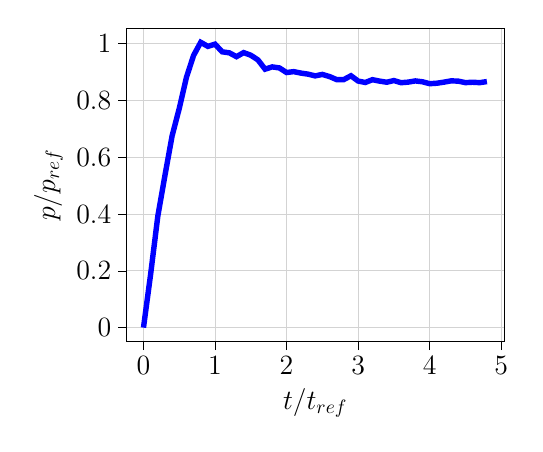
\begin{tikzpicture}[scale=0.7, font=\Large]

\definecolor{lightgray}{RGB}{211,211,211}

\begin{axis}[
tick align=outside,
tick pos=left,
x grid style={lightgray},
xlabel={\(\displaystyle t/t_{ref}\)},
xmajorgrids,
xmin=-0.24, xmax=5.04,
xtick style={color=black},
y grid style={lightgray},
ylabel={\(\displaystyle p/p_{ref}\)},
ymajorgrids,
ymin=-0.0502281761912294, ymax=1.05479170001582,
ytick style={color=black}
]
\addplot [line width=2.8pt, blue]
table {%
0 0
0.1 0.188445766752718
0.2 0.391947508110223
0.3 0.535895204930158
0.4 0.675176372415468
0.5 0.771710290038251
0.6 0.880899367078848
0.7 0.958412412909037
0.8 1.00456352382459
0.9 0.990324948221893
1 0.998054606057314
1.1 0.971102817197564
1.2 0.967556258546069
1.3 0.954084839144053
1.4 0.968359167181806
1.5 0.959116405852193
1.6 0.942617944583139
1.7 0.910026091662552
1.8 0.918049400613525
1.9 0.914348525898006
2 0.898192078875057
2.1 0.901362856789026
2.2 0.896214438996315
2.3 0.892511564645737
2.4 0.886358846124087
2.5 0.891502924804546
2.6 0.884023936770732
2.7 0.873345919605794
2.8 0.873412882862689
2.9 0.886829564180904
3 0.868198311002277
3.1 0.863129333961807
3.2 0.873000347785484
3.3 0.867964509851173
3.4 0.864042793812506
3.5 0.869939165930708
3.6 0.862387111210862
3.7 0.864402846886308
3.8 0.868605632794512
3.9 0.865597652226709
4 0.8589197342603
4.1 0.860522133055493
4.2 0.864358319941601
4.3 0.868875836425173
4.4 0.867843224744737
4.5 0.862641238764823
4.6 0.863963070087864
4.7 0.862565672752955
4.8 0.866328855022948
};
\end{axis}

\end{tikzpicture}

  \hspace{0.5cm}
  % This file was created with tikzplotlib v0.10.1.
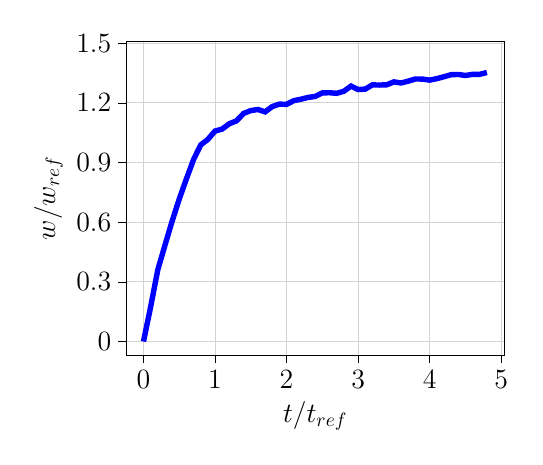
\begin{tikzpicture}[scale=0.7, font=\Large]

\definecolor{lightgray}{RGB}{211,211,211}

\begin{axis}[
tick align=outside,
tick pos=left,
x grid style={lightgray},
xlabel={\(\displaystyle t/t_{ref}\)},
xmajorgrids,
xmin=-0.24, xmax=5.04,
xtick style={color=black},
y grid style={lightgray},
ytick distance=0.3,
ylabel={\(\displaystyle w/w_{ref}\)},
ymajorgrids,
ymin=-0.0676150128188689, ymax=1.51,
ytick style={color=black}
]
\addplot [line width=2.8pt, blue]
table {%
0 0
0.1 0.174099460537345
0.2 0.36037093622801
0.3 0.483736302329922
0.4 0.604657400483929
0.5 0.71627362525909
0.6 0.817741763252065
0.7 0.914673087058184
0.8 0.988043835003288
0.9 1.01615749619579
1 1.05781999647227
1.1 1.06795558571426
1.2 1.09487671410362
1.3 1.10903211791217
1.4 1.14665606861212
1.5 1.16093104459679
1.6 1.16625499737314
1.7 1.15430886393875
1.8 1.18121700420342
1.9 1.19330912726223
2 1.19206895215774
2.1 1.21057291458408
2.2 1.21798236109138
2.3 1.22691783387849
2.4 1.23188777939765
2.5 1.24970648339836
2.6 1.25053556512246
2.7 1.24766343959738
2.8 1.2578584515492
2.9 1.28381515930564
3 1.26659534216305
3.1 1.26894556444263
3.2 1.29005564497642
3.3 1.28918001813621
3.4 1.29050708947248
3.5 1.30520754884353
3.6 1.29951568143079
3.7 1.30872862561227
3.8 1.31974418932991
3.9 1.31922767023963
4 1.31398053120865
4.1 1.32143831069796
4.2 1.33095372857038
4.3 1.34126355648886
4.4 1.34234868328863
4.5 1.33716954069027
4.6 1.34310704227726
4.7 1.34310814299716
4.8 1.35230025637738
};
\end{axis}

\end{tikzpicture}

  \caption{Two quantities of interest for the parallel fracture problem. On the left, the time series of the pressure at the injection point, on the right, the fracture aperture. Both plots show results scaled by reference values, calculated at the onset of propagation.}  
  \label{fig:parallel_fracs_charts}
\end{figure}


\begin{figure}[h]
\begin{subfigure}{.45\textwidth}
  \centering
  \includegraphics[width=\linewidth]{Chapter4/figures/3D/new_t_0.png}
  \caption{}
  \label{fig:parallel_t_0}
\end{subfigure}%
\hspace{1cm}
\begin{subfigure}{.45\textwidth}
  \centering
  \includegraphics[width=\linewidth]{Chapter4/figures/3D/new_t_30.png}
  \caption{}
  \label{fig:parallel_t_1}
\end{subfigure}%

\begin{subfigure}{.45\textwidth}
  \centering
  \includegraphics[width=\linewidth]{Chapter4/figures/3D/new_t_60.png}
  \caption{}
  \label{fig:parallel_t_2}
\end{subfigure}
\hspace{0.85cm}
\begin{subfigure}{.45\textwidth}
  \centering
  \includegraphics[width=\linewidth]{Chapter4/figures/3D/new_t_90.png}
  \caption{}
  \label{fig:parallel_t_3}
\end{subfigure}
  \caption{Snapshots of the simulated propagation. The left side of the figures shows the discrete fracture colored in grayscale according to the aperture and the subdomain colored according the damage value. The right side shows the pressure field in the global domain. (a) Snapshot $t/t_{ref} = 0$; (b) $t/t_{ref} = 1.5$; (c) $t/t_{ref} = 3$; and (d) $t/t_{ref} = 4.5$. } 
  \label{fig:parallel_snapshots}
\end{figure}

\FloatBarrier

\subsection{Merging two circular fractures}

The second problem deals with the case of in-plane fracture merging. In general, fracture merging is one of the most difficult behaviors to simulate with discrete fracture approaches. That is due to the interaction between the stress fields of two fracture fronts, which makes most attempts to extract a stress intensity factor innacurate. In practice, these situation may happen when fracking wells are drilled parallel to each other. 

For problems involving crack merging, the phase-field approach becomes handy, allowing for the computation of crack advances through the solution of PDEs that are independent of the fracture topology.
The multi-resolution approach explore this advantage, keeping a phase-field description around the fracture front and removing the limitations of discrete methods.

Since this problem deals with in-plane merging, getting the discrete fracture planes from the phase-field values is straightforward. However, it is important to mention that this can be a challenge in the case of non-planar merging.

The problem under consideration consists of two parallel fractures, initally of circular shape, embedded in a poroelastic matrix. Both are injected with a viscous fluid and propagate radially, eventually merging. An schematic of the geometry is shown in Figure \ref{fig:merging_schematic}, with the dimensions listed in Table \ref{merging_measures}. As in the previous problem, the far-field boundary conditions are assumed to be homogenous for pressures and displacements. 

As for the discretization, the coarser global mesh consists of a structured grid that is refined near the fracture planes, with an element size of around 0.095m in the width direction and 0.15m in the other directions. The local mesh is 5 times smaller and the regularization length used in the phase-field subproblem is 0.05m. Importantly, the local domain consists of all local elements within a distance of 1m to the fracture front. Initally, they consist of two separate torus, but they eventually merge as the cracks get closer. As for the time-step, it is uniformly set to 0.01s.

The simulated behavior is depicted in Figure \ref{fig:merge_snapshots}, which shows the expected behavior, which the cracks growing perfectly as circles until they approach each other and merge. After the merge, the most concave part of the crack grows and opens up until the pressure drops enough for the propagation to arrest. While there is not reference solution to compare, at least qualitatively, the results make sense. As for the previous problem, the times series for the aperture and pressure in the injection point are shown in Figure \ref{fig:merging_charts}. The reference values used to make these charts nondimensional are given in Table \ref{merging_refs}.

\begin{table}[ht]
  \centering
  \caption{Domain dimensions}
  \begin{tabular}[t]{lccccccc}
  \hline
  &$d_1$&$d_2$&$d_3$&$L_x$&$L_y$&$L_z$&$r$\\  
  \hline
  Value (m) & 6.5 & 7.0 & 6.5 & 8.0 & 20.0 & 5.0 & 1.5\\
  \hline
  \end{tabular}
  \label{merging_measures}
\end{table}%

\begin{table}[ht]
  \centering
  \caption{Reference values used in the time series plots.}
  \begin{tabular}[t]{lcc}
  \hline
  &Value &Unit \\
  \hline
  $p_{ref}$&520&MPa\\
  $w_{ref}$&7.0$\times 10^{-4}$&m\\
  $t_{ref}$&10&$\text{s}$\\
  \hline
  \end{tabular}
  \label{merging_refs}
\end{table}%

\begin{figure}[ht]
  \centering
  \begin{tikzpicture}
      \node {\pgfimage[interpolate=false,width=.8\textwidth]{Chapter4/figures/merging/merging_schematic.png}};
      \draw (0.0\textwidth,0.07\textwidth) node {\large$r$};
      \draw (0.37\textwidth,0.12\textwidth) node {\large$L_x$};
      \draw (0.04\textwidth,-0.25\textwidth) node {\large$L_y$};
      \draw (0.42\textwidth,-0.07\textwidth) node {\large$L_z$};
      \draw (-0.25\textwidth,0.25\textwidth) node {\large$d_1$};
      \draw (-0.03\textwidth,0.25\textwidth) node {\large$d_2$};
      \draw (0.2\textwidth,0.25\textwidth) node {\large$d_3$};
  \end{tikzpicture}
  \caption{Schematic of the geometry for the merging problem.}
  \label{fig:merging_schematic}
\end{figure}


\begin{figure}[h]
\noindent% This file was created with tikzplotlib v0.10.1.
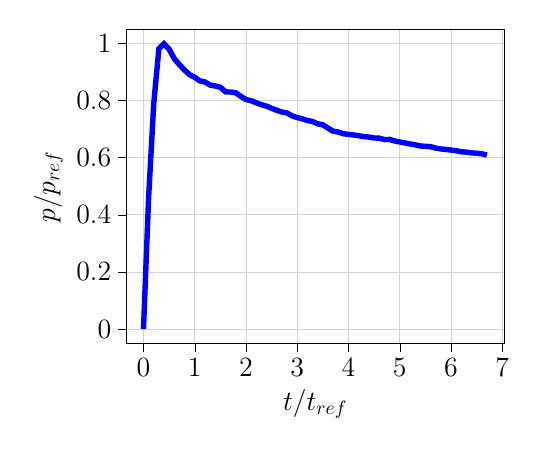
\begin{tikzpicture}[scale=0.7, font=\Large]

\definecolor{lightgray}{RGB}{211,211,211}

\begin{axis}[
tick align=outside,
tick pos=left,
x grid style={lightgray},
xlabel={\(\displaystyle t/t_{ref}\)},
xmajorgrids,
xmin=-0.335, xmax=7.035,
xtick style={color=black},
y grid style={lightgray},
ylabel={\(\displaystyle p/p_{ref}\)},
ymajorgrids,
ymin=-0.0498825329280283, ymax=1.0475331914886,
ytick style={color=black}
]
\addplot [line width=2.8pt, blue]
table {%
0 0
0.1 0.45951217560765
0.2 0.788592266536983
0.3 0.979658043857808
0.4 0.997650658560567
0.5 0.978785067303964
0.6 0.945971757956235
0.7 0.924877167218727
0.8 0.905966129538245
0.9 0.889602759640749
1 0.880357526928354
1.1 0.867671216379265
1.2 0.864233448832077
1.3 0.853114312789821
1.4 0.850108135287821
1.5 0.845620481022948
1.6 0.829505321551291
1.7 0.82892647153026
1.8 0.826514080553166
1.9 0.813655142687903
2 0.802768783688767
2.1 0.798543387344519
2.2 0.791408224631453
2.3 0.784592950157044
2.4 0.779669735090534
2.5 0.771982941261582
2.6 0.764935123584626
2.7 0.759180136109881
2.8 0.755819802453577
2.9 0.745394700232725
3 0.739759343297616
3.1 0.73509236716247
3.2 0.729345702728615
3.3 0.725778734141958
3.4 0.717687645906032
3.5 0.714371573361759
3.6 0.702688940886406
3.7 0.692071117257683
3.8 0.689075788412169
3.9 0.683018346545578
4 0.680940241480926
4.1 0.678761582675207
4.2 0.676155909908243
4.3 0.67303862482668
4.4 0.67141982291266
4.5 0.668213339195578
4.6 0.667744559568312
4.7 0.662721346127251
4.8 0.663129635213632
4.9 0.657892335911165
5 0.654296951897791
5.1 0.650863757765831
5.2 0.647428666367983
5.3 0.644241597549297
5.4 0.640318013987773
5.5 0.638947287170507
5.6 0.638052591816986
5.7 0.632877744620429
5.8 0.629874714646489
5.9 0.62812562862508
6 0.625989632848015
6.1 0.623727478456361
6.2 0.61994558051626
6.3 0.618837276024664
6.4 0.616144894474259
6.5 0.614945973289227
6.6 0.612979236533847
6.7 0.60828213805131
};
\end{axis}

\end{tikzpicture}
\hspace{0.5cm}
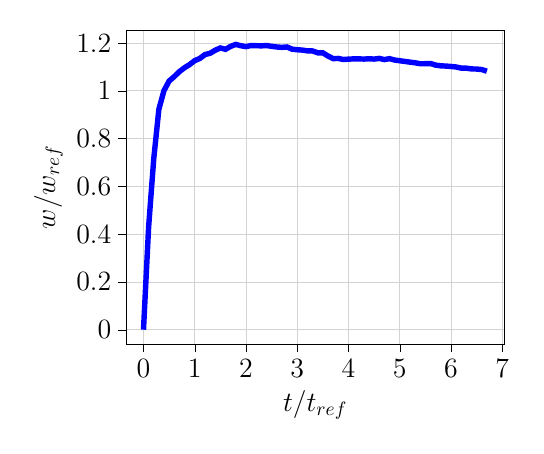
\begin{tikzpicture}[scale=0.7, font=\Large]

\definecolor{lightgray}{RGB}{211,211,211}

\begin{axis}[
tick align=outside,
tick pos=left,
x grid style={lightgray},
xlabel={\(\displaystyle t/t_{ref}\)},
xmajorgrids,
xmin=-0.335, xmax=7.035,
xtick style={color=black},
y grid style={lightgray},
ylabel={\(\displaystyle w/w_{ref}\)},
ymajorgrids,
ymin=-0.0597293287257296, ymax=1.25431590324032,
ytick style={color=black}
]
\addplot [line width=2.8pt, blue]
table {%
0 0
0.1 0.42960065054532
0.2 0.715136605775466
0.3 0.922750840112107
0.4 1.0013207791429
0.5 1.0411598779676
0.6 1.05982581607324
0.7 1.08050584575762
0.8 1.09671277193648
0.9 1.11032136558952
1 1.12663033076329
1.1 1.13590704337549
1.2 1.15199446917512
1.3 1.15745805434228
1.4 1.17029484955157
1.5 1.1797256365628
1.6 1.17401971466754
1.7 1.18622756700584
1.8 1.19458657451459
1.9 1.18892597827636
2 1.18545966357443
2.1 1.18983889045998
2.2 1.18920351864721
2.3 1.18850491342986
2.4 1.18987192915262
2.5 1.18655089416824
2.6 1.18376216613162
2.7 1.18232996709817
2.8 1.18384178574721
2.9 1.1745917982695
3 1.17218634899917
3.1 1.17081354140302
3.2 1.1674404732521
3.3 1.16714196039589
3.4 1.15942128056545
3.5 1.15905443325056
3.6 1.14598602032622
3.7 1.13512321674529
3.8 1.13577811166775
3.9 1.13137169873407
4 1.13287911123356
4.1 1.13401684532316
4.2 1.13401065495831
4.3 1.13319092621984
4.4 1.13446327534522
4.5 1.13314924992658
4.6 1.13590775886393
4.7 1.13102049244932
4.8 1.13486709640336
4.9 1.12912798009531
5 1.12617496099899
5.1 1.12326496239068
5.2 1.1202902089975
5.3 1.11761318780537
5.4 1.11361031173121
5.5 1.11379000169957
5.6 1.11459022130972
5.7 1.10788856842442
5.8 1.1048189314348
5.9 1.10389204151723
6 1.10216294677504
6.1 1.10006683973921
6.2 1.09525678021556
6.3 1.09503757716002
6.4 1.09193800888068
6.5 1.09139905221393
6.6 1.08928999986265
6.7 1.08233446321413
};
\end{axis}

\end{tikzpicture}
\caption{Two quantities of interest for the merging fracture problem. On the left, the time series of the pressure at the injection point, on the right, the fracture aperture. Both plots show results scaled by reference values, calculated at the onset of propagation.}  
\label{fig:merging_charts}
\end{figure}


\begin{figure}[h]
\begin{subfigure}{.45\textwidth}
  \centering
  \includegraphics[width=\linewidth]{Chapter4/figures/merging/merging_t_1.png}
  \caption{}
  \label{fig:merge_t_0}
\end{subfigure}%
\hspace{1cm}
\begin{subfigure}{.45\textwidth}
  \centering
  \includegraphics[width=\linewidth]{Chapter4/figures/merging/merging_t_14.png}
  \caption{}
  \label{fig:merge_t_1}
\end{subfigure}%

\begin{subfigure}{.45\textwidth}
  \centering
  \includegraphics[width=\linewidth]{Chapter4/figures/merging/merging_t_27.png}
  \caption{}
  \label{fig:merge_t_2}
\end{subfigure}
\hspace{0.85cm}
\begin{subfigure}{.45\textwidth}
  \centering
  \includegraphics[width=\linewidth]{Chapter4/figures/merging/merging_t_35.png}
  \caption{}
  \label{fig:merge_t_3}
\end{subfigure}

\begin{subfigure}{.45\textwidth}
  \centering
  \includegraphics[width=\linewidth]{Chapter4/figures/merging/merging_t_42.png}
  \caption{}
  \label{fig:merge_t_4}
\end{subfigure}
\hspace{0.85cm}
\begin{subfigure}{.45\textwidth}
  \centering
  \includegraphics[width=\linewidth]{Chapter4/figures/merging/merging_t_67.png}
  \caption{}
  \label{fig:merge_t_5}
\end{subfigure}
  \caption{Snapshots of the simulated propagation. The discrete fracture is colored in grayscale according to the aperture and the subdomain colored according the damage value. (a) Snapshot $t/t_{ref} = 0$; (b) $t/t_{ref} = 1.3$; (c) $t/t_{ref} = 2.6$; (d) $t/t_{ref} = 3.9$; (e) $t/t_{ref} = 5.2$; and (f) $t/t_{ref} = 6.5$. } 
  \label{fig:merge_snapshots}  
\end{figure}

\FloatBarrier



 % Start with '\chapter{Title}'

%-----------------------------------------------------------------------------%
% BIBLIOGRAPHY -- uncomment \nocite{*} to include items in 'mybib.bib' file
% that aren't cited in the text.  Change the style to match your
% discipline's standards.  Of course, if your bibliography file isn't called
% 'mybib.bib' you might want to change that here too :)
%-----------------------------------------------------------------------------%
%\nocite{*} - if you use this it will put EVERYTHING in your .bib file into the references even if you don't cite it in the text
\bibliographystyle{unsrtnat} %Formats bibliography
\cleardoublepage
\normalbaselines %Fixes spacing of bibliography
\addcontentsline{toc}{chapter}{Bibliography} %adds Bibliography to your table of contents
\bibliography{Bibliography/References} %your bibliography file - change the path if needed
%-----------------------------------------------------------------------------%

%-----------------------------------------------------------------------------%
% BIOGRAPHY -- Start file with '\biography'.  Mandatory for Ph.D.
%-----------------------------------------------------------------------------%
\biography

Andre Costa earned his B.S. degree in Mechanical Engineering and M.S. degree in Mathematics from Universidade Federal de Minas Gerais, in Brazil. He joined the Department of 
Mechanical Engineering and Materials Science at Duke University in 
2018 as a graduate research assistant. His Ph.D. degree was awarded in the Fall of 2023 and he will be working as a Software Engineer at Cadence Design Systems Inc.


%-----------------------------------------------------------------------------
% You're done :)
\end{document}
